% Options for packages loaded elsewhere
\PassOptionsToPackage{unicode}{hyperref}
\PassOptionsToPackage{hyphens}{url}
\documentclass[
]{book}
\usepackage{xcolor}
\usepackage{amsmath,amssymb}
\setcounter{secnumdepth}{5}
\usepackage{iftex}
\ifPDFTeX
  \usepackage[T1]{fontenc}
  \usepackage[utf8]{inputenc}
  \usepackage{textcomp} % provide euro and other symbols
\else % if luatex or xetex
  \usepackage{unicode-math} % this also loads fontspec
  \defaultfontfeatures{Scale=MatchLowercase}
  \defaultfontfeatures[\rmfamily]{Ligatures=TeX,Scale=1}
\fi
\usepackage{lmodern}
\ifPDFTeX\else
  % xetex/luatex font selection
\fi
% Use upquote if available, for straight quotes in verbatim environments
\IfFileExists{upquote.sty}{\usepackage{upquote}}{}
\IfFileExists{microtype.sty}{% use microtype if available
  \usepackage[]{microtype}
  \UseMicrotypeSet[protrusion]{basicmath} % disable protrusion for tt fonts
}{}
\makeatletter
\@ifundefined{KOMAClassName}{% if non-KOMA class
  \IfFileExists{parskip.sty}{%
    \usepackage{parskip}
  }{% else
    \setlength{\parindent}{0pt}
    \setlength{\parskip}{6pt plus 2pt minus 1pt}}
}{% if KOMA class
  \KOMAoptions{parskip=half}}
\makeatother
\usepackage{color}
\usepackage{fancyvrb}
\newcommand{\VerbBar}{|}
\newcommand{\VERB}{\Verb[commandchars=\\\{\}]}
\DefineVerbatimEnvironment{Highlighting}{Verbatim}{commandchars=\\\{\}}
% Add ',fontsize=\small' for more characters per line
\usepackage{framed}
\definecolor{shadecolor}{RGB}{248,248,248}
\newenvironment{Shaded}{\begin{snugshade}}{\end{snugshade}}
\newcommand{\AlertTok}[1]{\textcolor[rgb]{0.94,0.16,0.16}{#1}}
\newcommand{\AnnotationTok}[1]{\textcolor[rgb]{0.56,0.35,0.01}{\textbf{\textit{#1}}}}
\newcommand{\AttributeTok}[1]{\textcolor[rgb]{0.13,0.29,0.53}{#1}}
\newcommand{\BaseNTok}[1]{\textcolor[rgb]{0.00,0.00,0.81}{#1}}
\newcommand{\BuiltInTok}[1]{#1}
\newcommand{\CharTok}[1]{\textcolor[rgb]{0.31,0.60,0.02}{#1}}
\newcommand{\CommentTok}[1]{\textcolor[rgb]{0.56,0.35,0.01}{\textit{#1}}}
\newcommand{\CommentVarTok}[1]{\textcolor[rgb]{0.56,0.35,0.01}{\textbf{\textit{#1}}}}
\newcommand{\ConstantTok}[1]{\textcolor[rgb]{0.56,0.35,0.01}{#1}}
\newcommand{\ControlFlowTok}[1]{\textcolor[rgb]{0.13,0.29,0.53}{\textbf{#1}}}
\newcommand{\DataTypeTok}[1]{\textcolor[rgb]{0.13,0.29,0.53}{#1}}
\newcommand{\DecValTok}[1]{\textcolor[rgb]{0.00,0.00,0.81}{#1}}
\newcommand{\DocumentationTok}[1]{\textcolor[rgb]{0.56,0.35,0.01}{\textbf{\textit{#1}}}}
\newcommand{\ErrorTok}[1]{\textcolor[rgb]{0.64,0.00,0.00}{\textbf{#1}}}
\newcommand{\ExtensionTok}[1]{#1}
\newcommand{\FloatTok}[1]{\textcolor[rgb]{0.00,0.00,0.81}{#1}}
\newcommand{\FunctionTok}[1]{\textcolor[rgb]{0.13,0.29,0.53}{\textbf{#1}}}
\newcommand{\ImportTok}[1]{#1}
\newcommand{\InformationTok}[1]{\textcolor[rgb]{0.56,0.35,0.01}{\textbf{\textit{#1}}}}
\newcommand{\KeywordTok}[1]{\textcolor[rgb]{0.13,0.29,0.53}{\textbf{#1}}}
\newcommand{\NormalTok}[1]{#1}
\newcommand{\OperatorTok}[1]{\textcolor[rgb]{0.81,0.36,0.00}{\textbf{#1}}}
\newcommand{\OtherTok}[1]{\textcolor[rgb]{0.56,0.35,0.01}{#1}}
\newcommand{\PreprocessorTok}[1]{\textcolor[rgb]{0.56,0.35,0.01}{\textit{#1}}}
\newcommand{\RegionMarkerTok}[1]{#1}
\newcommand{\SpecialCharTok}[1]{\textcolor[rgb]{0.81,0.36,0.00}{\textbf{#1}}}
\newcommand{\SpecialStringTok}[1]{\textcolor[rgb]{0.31,0.60,0.02}{#1}}
\newcommand{\StringTok}[1]{\textcolor[rgb]{0.31,0.60,0.02}{#1}}
\newcommand{\VariableTok}[1]{\textcolor[rgb]{0.00,0.00,0.00}{#1}}
\newcommand{\VerbatimStringTok}[1]{\textcolor[rgb]{0.31,0.60,0.02}{#1}}
\newcommand{\WarningTok}[1]{\textcolor[rgb]{0.56,0.35,0.01}{\textbf{\textit{#1}}}}
\usepackage{longtable,booktabs,array}
\usepackage{calc} % for calculating minipage widths
% Correct order of tables after \paragraph or \subparagraph
\usepackage{etoolbox}
\makeatletter
\patchcmd\longtable{\par}{\if@noskipsec\mbox{}\fi\par}{}{}
\makeatother
% Allow footnotes in longtable head/foot
\IfFileExists{footnotehyper.sty}{\usepackage{footnotehyper}}{\usepackage{footnote}}
\makesavenoteenv{longtable}
\usepackage{graphicx}
\makeatletter
\newsavebox\pandoc@box
\newcommand*\pandocbounded[1]{% scales image to fit in text height/width
  \sbox\pandoc@box{#1}%
  \Gscale@div\@tempa{\textheight}{\dimexpr\ht\pandoc@box+\dp\pandoc@box\relax}%
  \Gscale@div\@tempb{\linewidth}{\wd\pandoc@box}%
  \ifdim\@tempb\p@<\@tempa\p@\let\@tempa\@tempb\fi% select the smaller of both
  \ifdim\@tempa\p@<\p@\scalebox{\@tempa}{\usebox\pandoc@box}%
  \else\usebox{\pandoc@box}%
  \fi%
}
% Set default figure placement to htbp
\def\fps@figure{htbp}
\makeatother
\setlength{\emergencystretch}{3em} % prevent overfull lines
\providecommand{\tightlist}{%
  \setlength{\itemsep}{0pt}\setlength{\parskip}{0pt}}
\usepackage[]{natbib}
\bibliographystyle{apalike}
\usepackage{booktabs}
\usepackage{amsthm}
\makeatletter
\def\thm@space@setup{%
  \thm@preskip=8pt plus 2pt minus 4pt
  \thm@postskip=\thm@preskip
}
\makeatother
\usepackage{float}
\usepackage{tabularray}
\usepackage[normalem]{ulem}
\usepackage{graphicx}
\usepackage{rotating}
\UseTblrLibrary{siunitx}
\NewTableCommand{\tinytableDefineColor}[3]{\definecolor{#1}{#2}{#3}}
\newcommand{\tinytableTabularrayUnderline}[1]{\underline{#1}}
\newcommand{\tinytableTabularrayStrikeout}[1]{\sout{#1}}
\usepackage{bookmark}
\IfFileExists{xurl.sty}{\usepackage{xurl}}{} % add URL line breaks if available
\urlstyle{same}
\hypersetup{
  pdftitle={POL342 R Tutorials},
  hidelinks,
  pdfcreator={LaTeX via pandoc}}

\title{POL342 R Tutorials}
\author{}
\date{\vspace{-2.5em}2026-09-12}

\begin{document}
\maketitle

{
\setcounter{tocdepth}{1}
\tableofcontents
}
\chapter*{Installing R and R Studio}\label{installing-r-and-r-studio}
\addcontentsline{toc}{chapter}{Installing R and R Studio}

Before the third week of class, please make sure to install the following software.

\begin{itemize}
\tightlist
\item
  \href{https://cran.rstudio.com/}{Installing R}
\item
  \href{https://posit.co/download/rstudio-desktop/}{Installing RStudio}
\end{itemize}

\chapter{Getting Started With Data Sets}\label{getting-started-with-data-sets}

Week 2 tutorial goals:

Using Microsoft Excel to understand

\begin{itemize}
\tightlist
\item
  Structure of datasets
\item
  Basics of a function
\end{itemize}

\section{Understanding data sets}\label{understanding-data-sets}

\begin{itemize}
\item
  Open ``STAR\_small.csv'' using Microsoft Excel.
\item
  What do you think this dataset is about?
\item
  How many rows and columns are there?
\item
  Look at the first column, ``classtype''.

  \begin{itemize}
  \tightlist
  \item
    What are the unique entries in the variable ``classtype''?
  \end{itemize}
\end{itemize}

\section{Basics of a function}\label{basics-of-a-function}

\subsection*{Consider the first variable in the data set}\label{consider-the-first-variable-in-the-data-set}
\addcontentsline{toc}{subsection}{Consider the first variable in the data set}

\begin{itemize}
\item
  Report the number of `small' and `regular' entries in the first variable using the \texttt{COUNTIFS()} function
\item
  To use functions, we need to know the \textbf{arguments} accepted in a function and how to specify each of these arguments
\item
  Description of \texttt{COUNTIFS()} from Microsoft's \href{https://support.microsoft.com/en-us/office/countifs-function-dda3dc6e-f74e-4aee-88bc-aa8c2a866842}{documentation}:
\end{itemize}

\begin{center}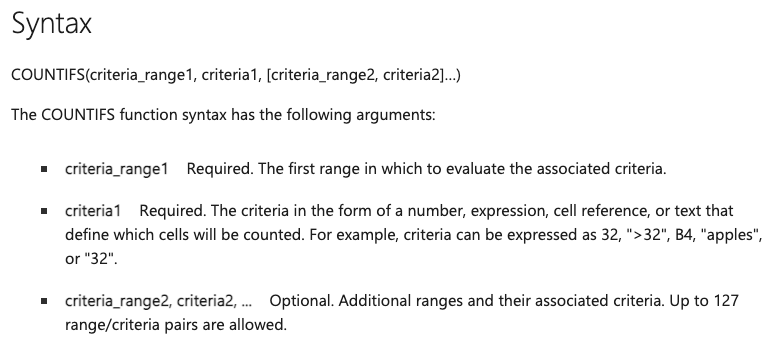
\includegraphics[width=0.7\linewidth]{images/w2_countif} \end{center}

\begin{itemize}
\tightlist
\item
  Try inserting this formula to a cell in the excel sheet:
\end{itemize}

\texttt{=COUNTIFS(A2:A50,"small")}

\begin{itemize}
\tightlist
\item
  And then this formula:
\end{itemize}

\texttt{=COUNTIFS(A2:A50,"regular")}

\subsection*{Next variables, ``reading'' and ``math''.}\label{next-variables-reading-and-math.}
\addcontentsline{toc}{subsection}{Next variables, ``reading'' and ``math''.}

\begin{itemize}
\item
  We are going to use the \texttt{AVERAGE()} function in Microsoft Excel.
\item
  Description of the function according to Microsoft's \href{https://support.microsoft.com/en-us/office/average-function-047bac88-d466-426c-a32b-8f33eb960cf6}{documentation}:
\end{itemize}

\begin{center}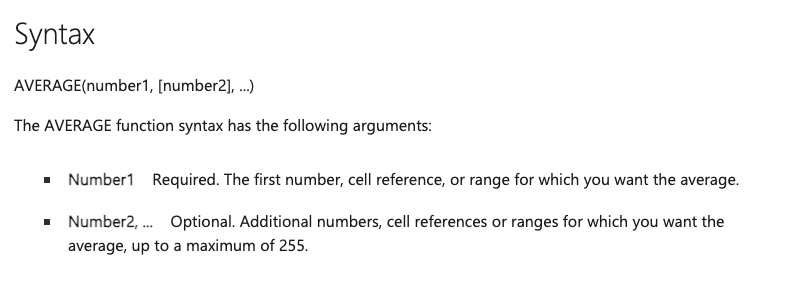
\includegraphics[width=0.7\linewidth]{images/w2_average} \end{center}

\begin{itemize}
\tightlist
\item
  Try inserting this formula to a cell in the excel sheet:
\end{itemize}

=AVERAGE(B2:B50)

\begin{itemize}
\item
  What is the formula to retrieve the mean for ``math''?
\item
  What is the formula to retrieve the mean for ``reading'' for the first 25 rows of the data?
\item
  Repeat the above three points for the median value using the \texttt{MEDIAN()} function.
\end{itemize}

\subsection*{Measures of dispersion}\label{measures-of-dispersion}
\addcontentsline{toc}{subsection}{Measures of dispersion}

\begin{itemize}
\tightlist
\item
  This is a box and whiskers plot of the reading and math variables.
\end{itemize}

\begin{center}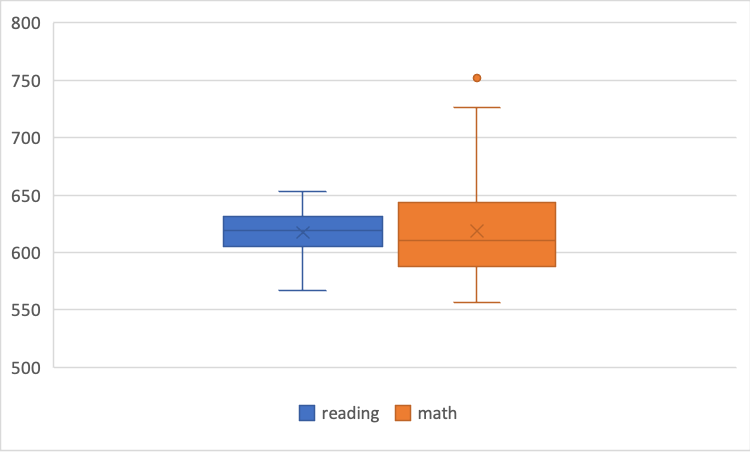
\includegraphics[width=0.7\linewidth]{images/w2_boxwhiskers} \end{center}

\begin{itemize}
\tightlist
\item
  The bottom and top of the box mark the 25th and 75th percentile of the data. Retrieve the 25th and 75th percentile of both variables using the \texttt{QUARTILE.INC(array,\ quartile)} function. The \texttt{quartile} argument takes values 0 (minimum), 1 (25th percentile) , 2 (50th percentile), 3 (75th percentile) , 4 (maximum).
\end{itemize}

Reading:\\
25th percentile --\\
75th percentile --

Math:\\
25th percentile --\\
75th percentile --

\begin{itemize}
\tightlist
\item
  The bottom and top of the whiskers mark the minimum and maximum value of the data if they are within 1.5 times of the interquartile range. Retrieve the maximum and minimum values using the \texttt{QUARTILE.INC()} or \texttt{MAX()} and \texttt{MIN()} functions.
\end{itemize}

Reading:\\
Minimum --\\
Maximum --

Math:\\
Minimum --\\
Maximum --

\begin{itemize}
\item
  Which variable do you think has a larger standard deviation---reading or math?
\item
  Retrieve the standard deviation using the function \texttt{STDEV.S()}.
\item
  Description of the function according to Microsoft's \href{https://support.microsoft.com/en-us/office/stdev-s-function-7d69cf97-0c1f-4acf-be27-f3e83904cc23}{documentation}:
\end{itemize}

\begin{center}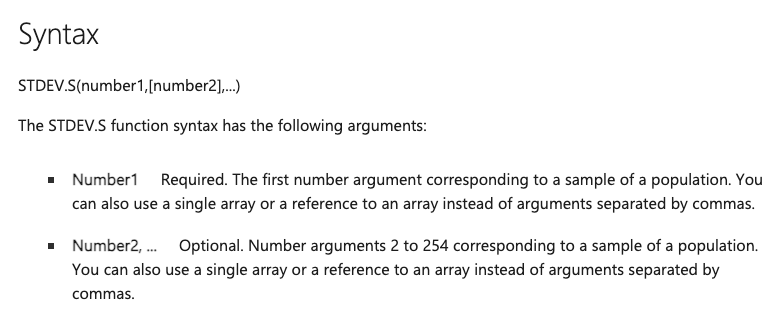
\includegraphics[width=0.7\linewidth]{images/w2_stdev} \end{center}

\chapter{Intro to R}\label{intro-to-r}

Week 3 tutorial goals:

\begin{itemize}
\tightlist
\item
  R Basics

  \begin{itemize}
  \tightlist
  \item
    Object types
  \item
    Packages
  \item
    Working directory
  \item
    Importing data
  \item
    Exploring data
  \end{itemize}
\end{itemize}

\section{RStudio}\label{rstudio}

\subsection*{What is R? What is coding?}\label{what-is-r-what-is-coding}
\addcontentsline{toc}{subsection}{What is R? What is coding?}

\begin{itemize}
\tightlist
\item
  Coding is a language that is fed directly into an interpreter.
\item
  Programming languages are fed into a computing system that reads the script and executes the commands.
\item
  Non-programming languages simply translates the programming language into its corresponding output, e.g.~Hypertext Markup Language (HTML). HTML is often used to display information on webpages.
\end{itemize}

\begin{center}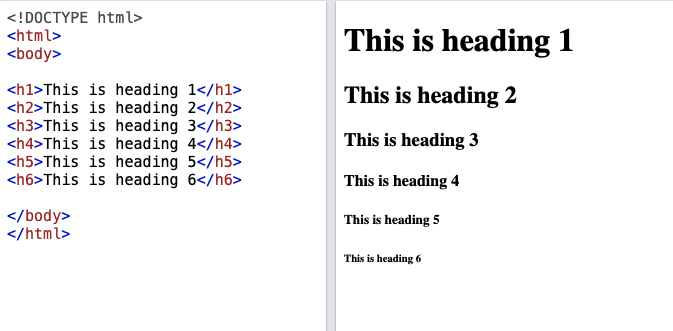
\includegraphics[width=0.7\linewidth]{images/w3_htmleg} \end{center}

\begin{itemize}
\tightlist
\item
  E.g. of other programming languages: JavaScript; Python; Mac Terminal (bash); Windows Command Prompt

  \begin{itemize}
  \tightlist
  \item
    \texttt{R} is a software for statistical computing. It is designed with particular processes that are tailored to statistical analysis and graphics. In order to initiate those processes, we write our commands in an R script for R to interpret and execute.
  \end{itemize}
\end{itemize}

\subsection*{Integrated Development Environment (IDE) editor: RStudio}\label{integrated-development-environment-ide-editor-rstudio}
\addcontentsline{toc}{subsection}{Integrated Development Environment (IDE) editor: RStudio}

RStudio is a software that makes R more user-friendly. If you run the software R, you see only a single panel, which is not very informative.

\begin{center}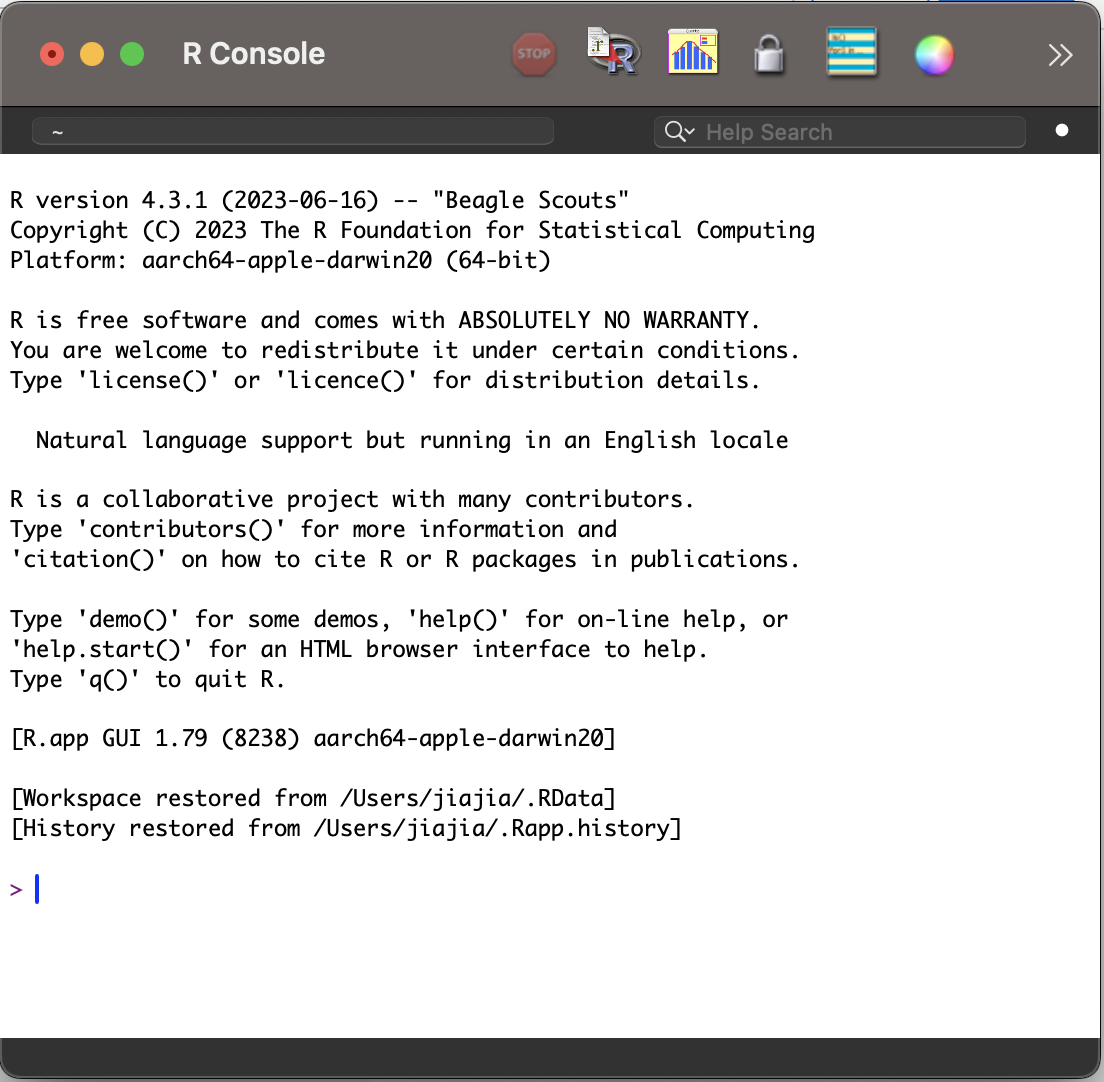
\includegraphics[width=0.7\linewidth]{images/w3_Rconsole} \end{center}

RStudio gives you more panels in addition to the R console (on the left) that displays information to support our use of R.

\begin{center}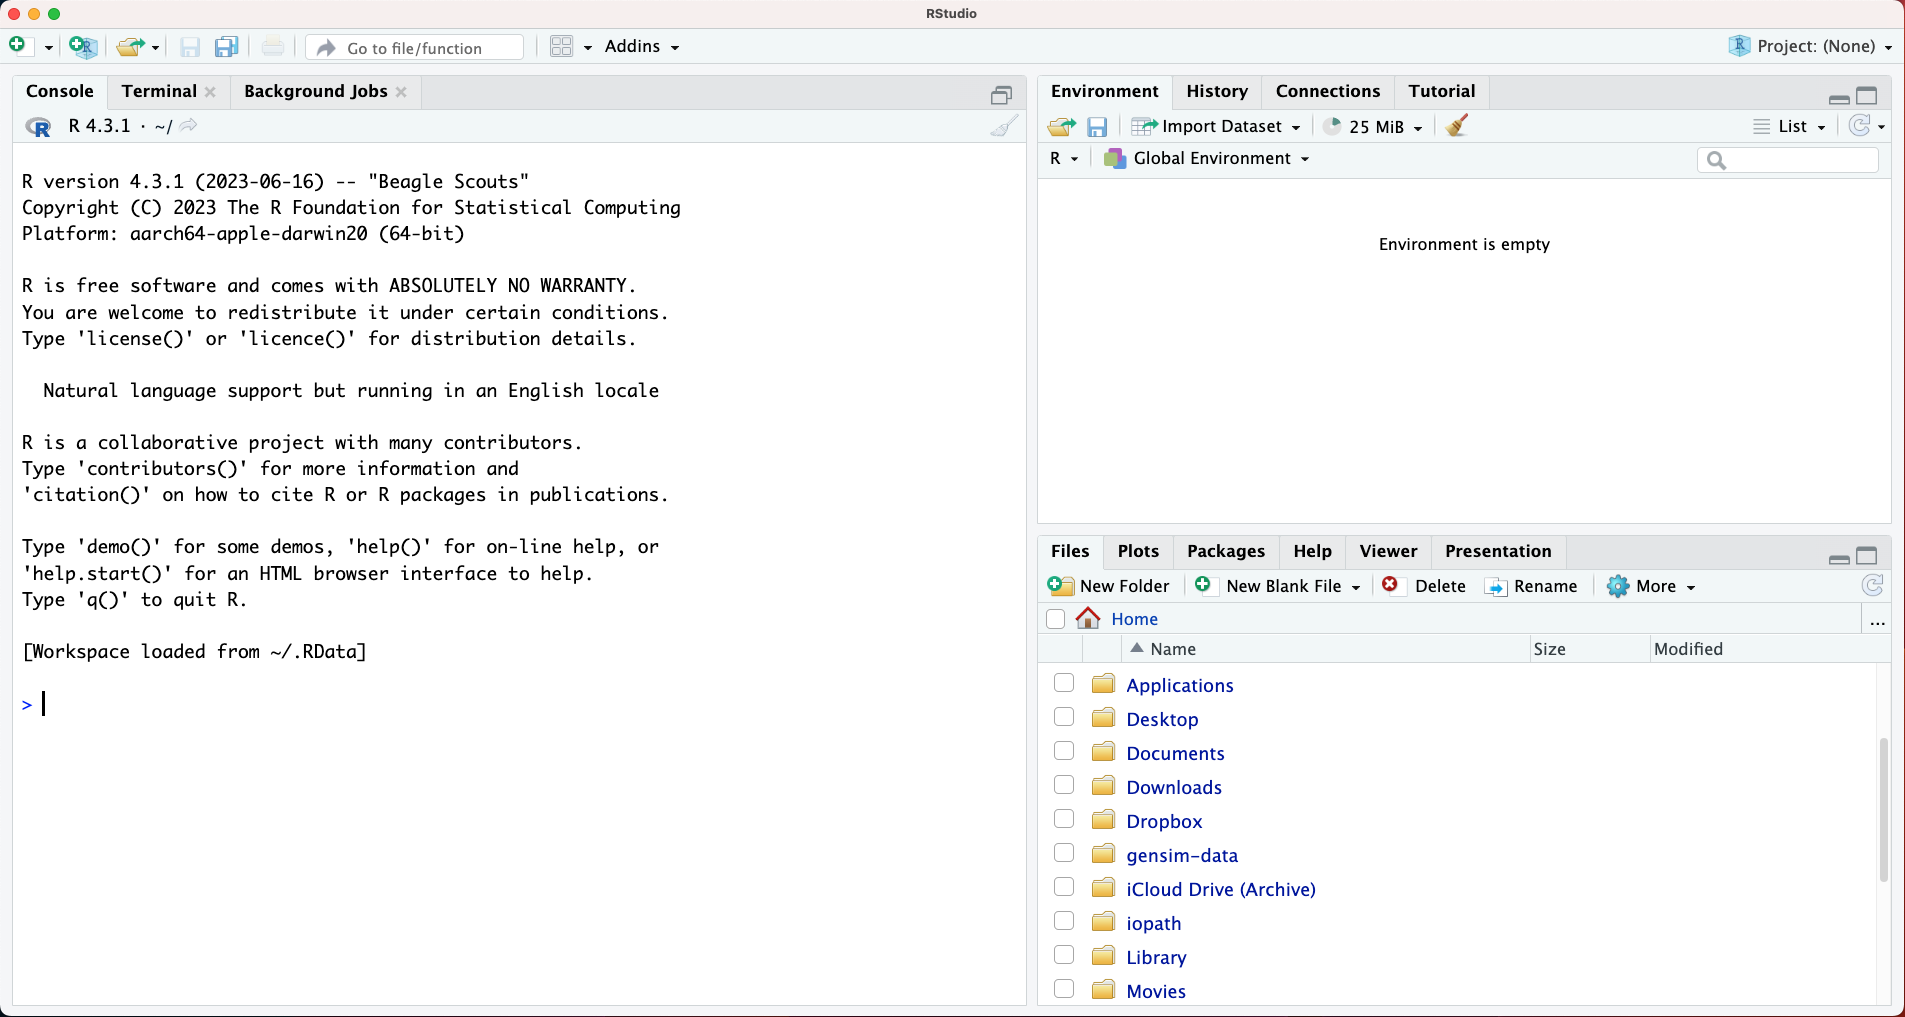
\includegraphics[width=0.9\linewidth]{images/w3_RStudio} \end{center}

\subsubsection*{Console}\label{console}
\addcontentsline{toc}{subsubsection}{Console}

\begin{center}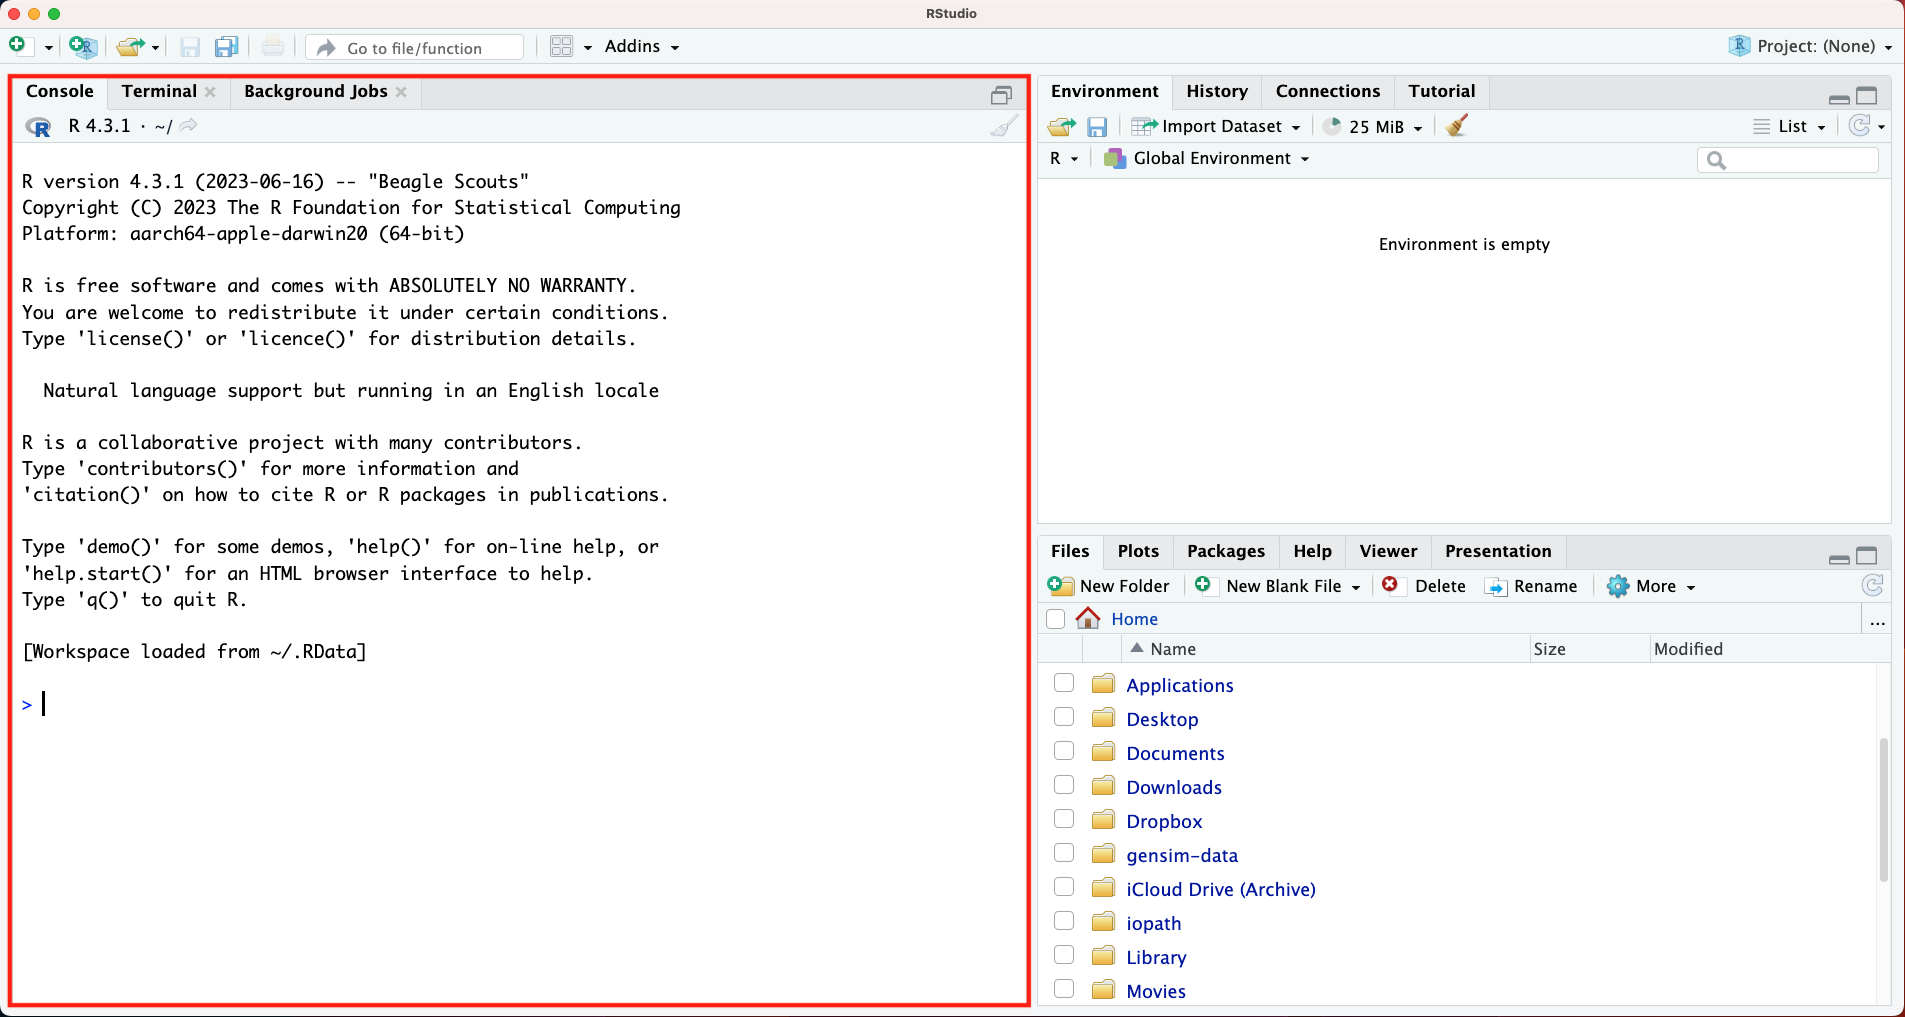
\includegraphics[width=0.9\linewidth]{images/w3_RStudio1} \end{center}

\subsubsection*{Environment}\label{environment}
\addcontentsline{toc}{subsubsection}{Environment}

The environment lists the objects you have saved and are able to ``call'' (i.e.~use in subsequent commands).

\begin{center}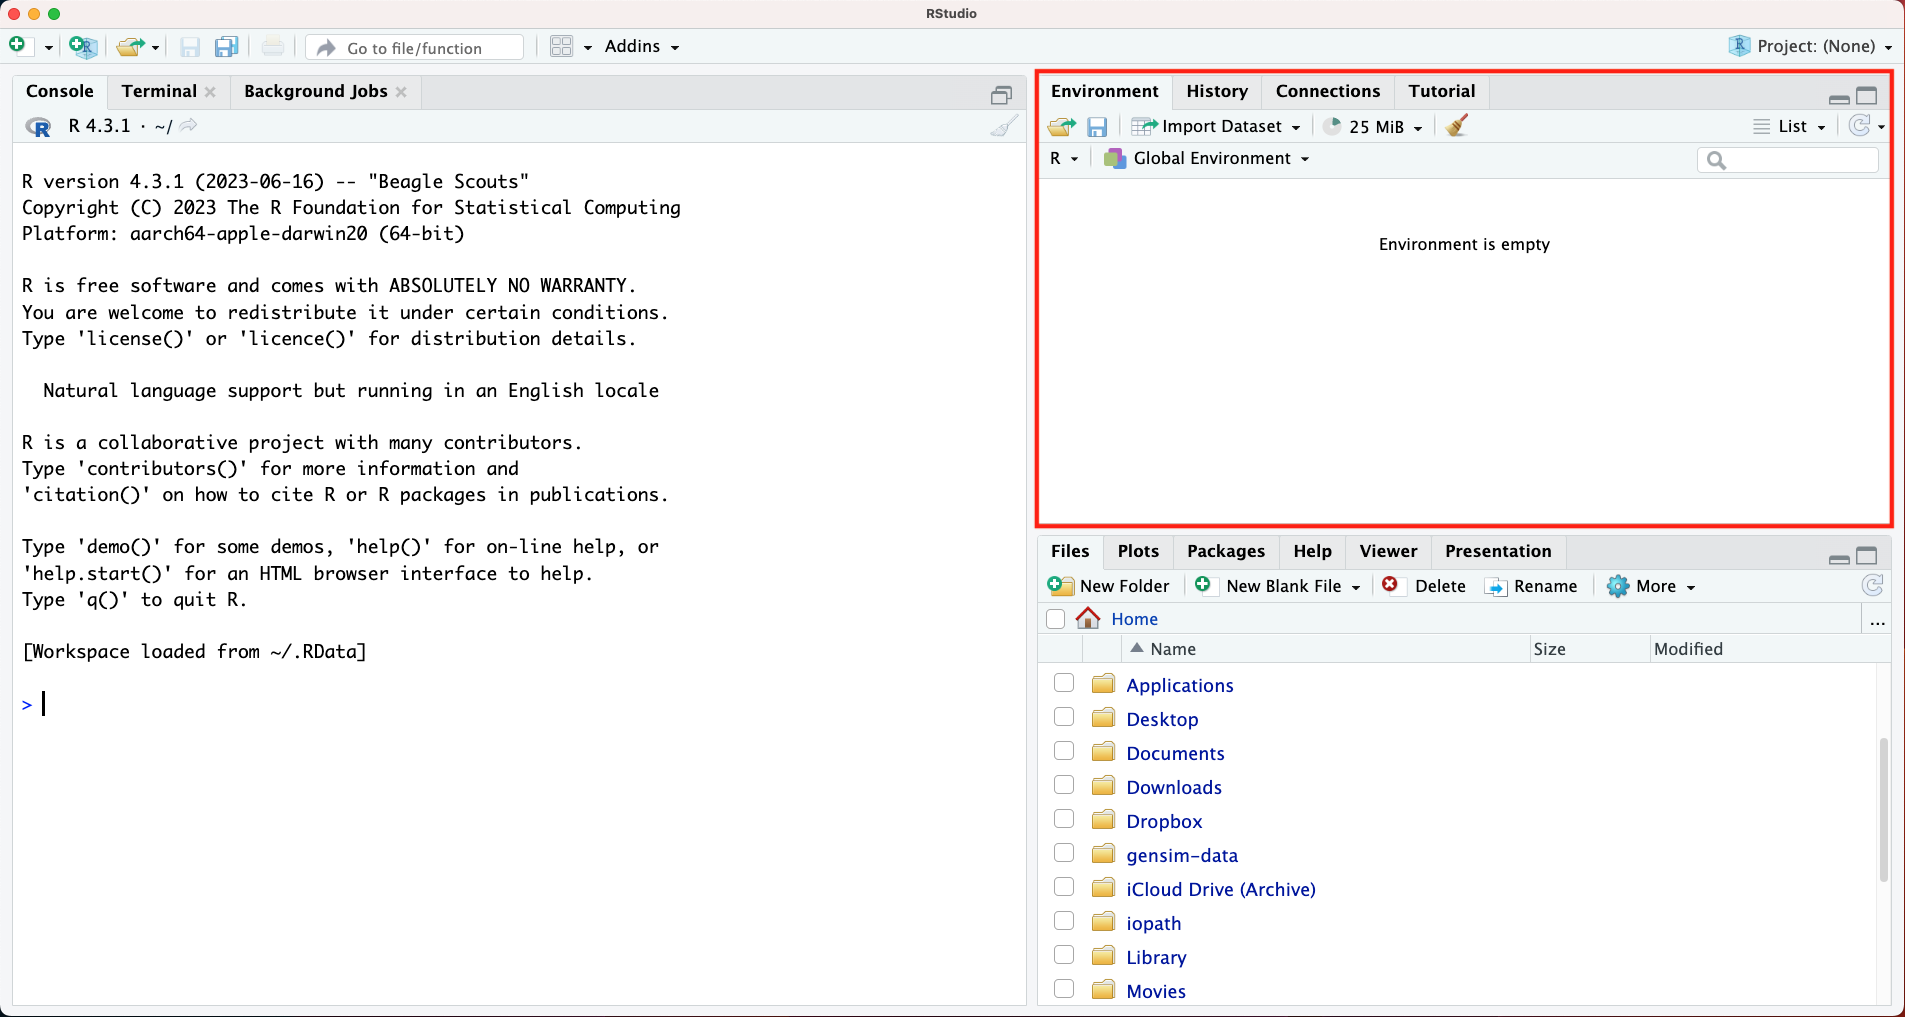
\includegraphics[width=0.9\linewidth]{images/w3_RStudio2} \end{center}

\subsubsection*{Files/Plots}\label{filesplots}
\addcontentsline{toc}{subsubsection}{Files/Plots}

\begin{center}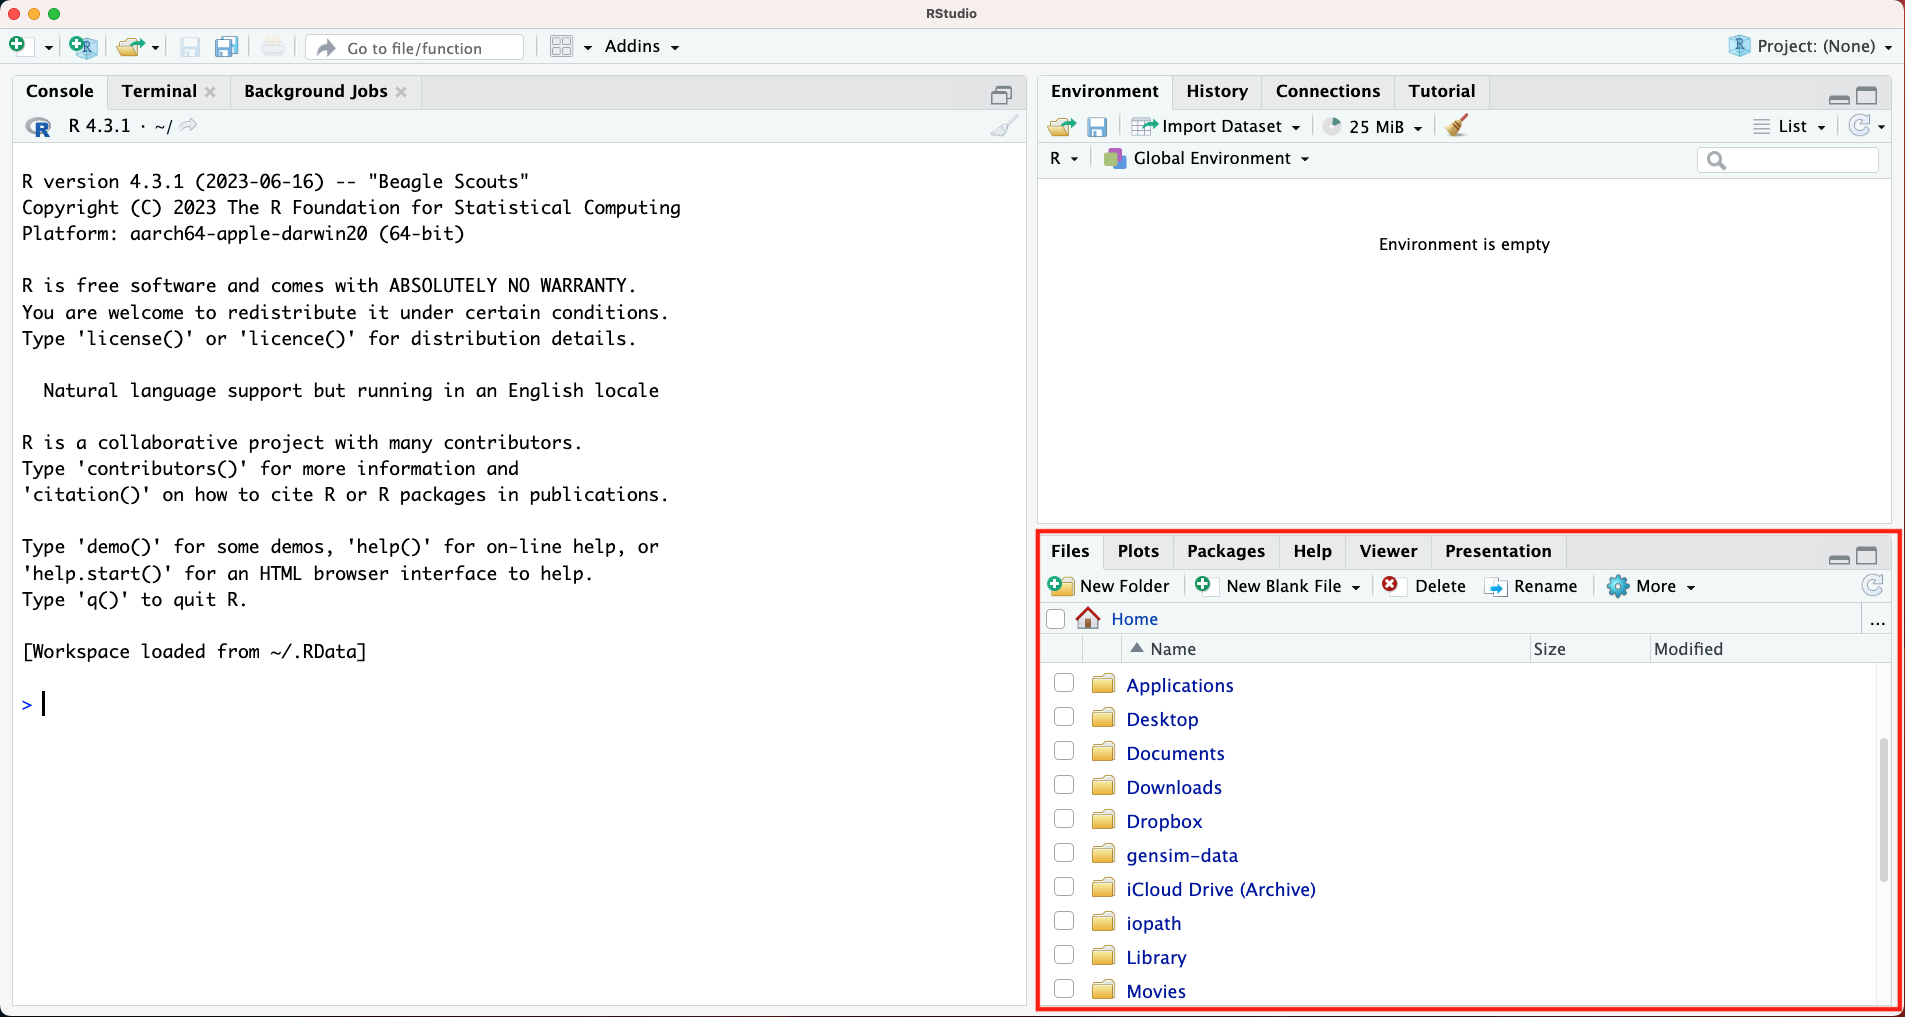
\includegraphics[width=0.9\linewidth]{images/w3_RStudio3} \end{center}

\subsubsection*{R Script}\label{r-script}
\addcontentsline{toc}{subsubsection}{R Script}

You can try to run codes in the console, but running codes linearly can be restricting, kind of like using a typewriter instead of a word document---you have to redo everything when you make a mistake.

\begin{center}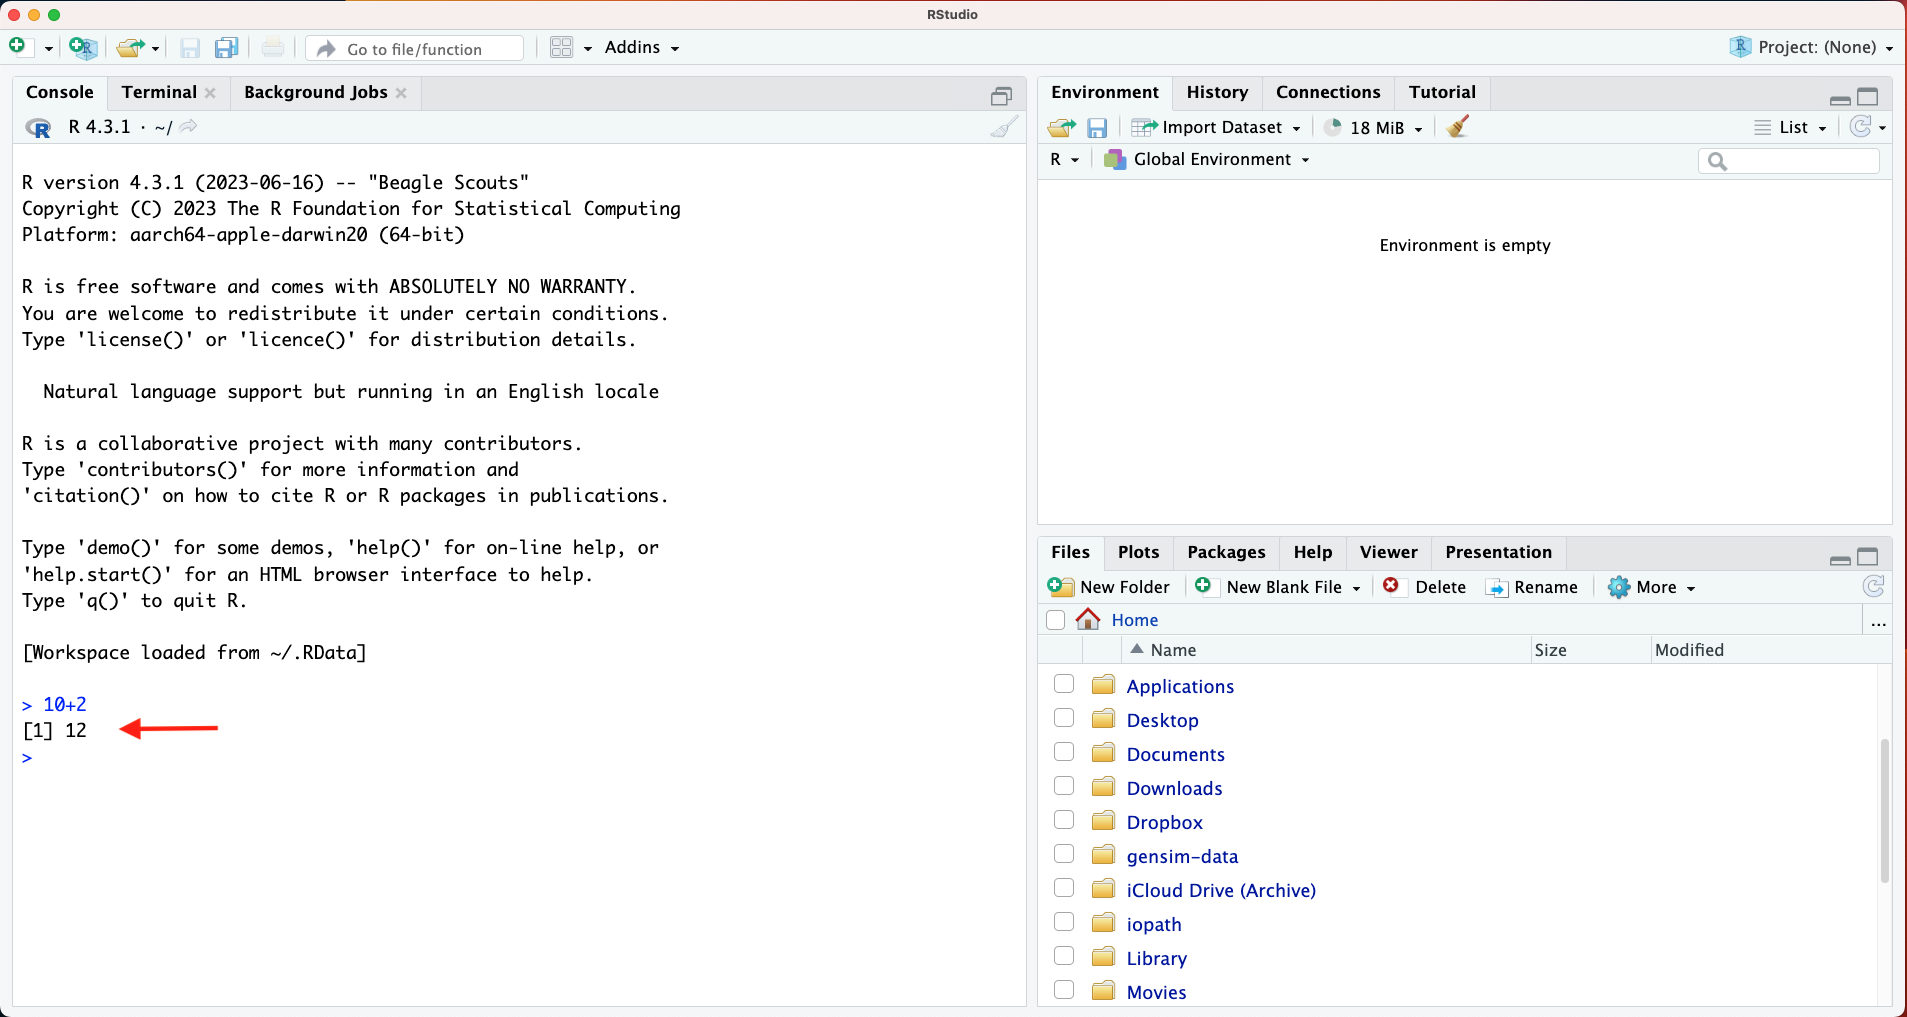
\includegraphics[width=0.9\linewidth]{images/w3_RStudio_console} \end{center}

In order to create our code document, we need the R script.

\begin{center}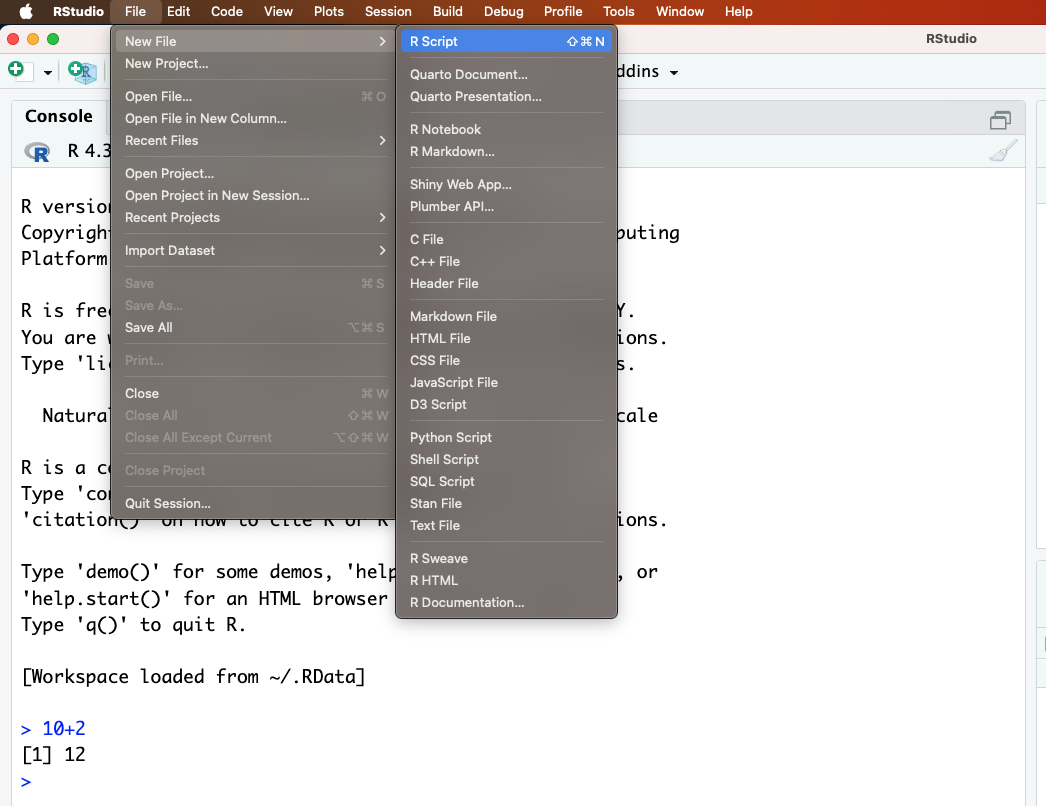
\includegraphics[width=0.9\linewidth]{images/w3_RStudio_Rfile} \end{center}

\begin{center}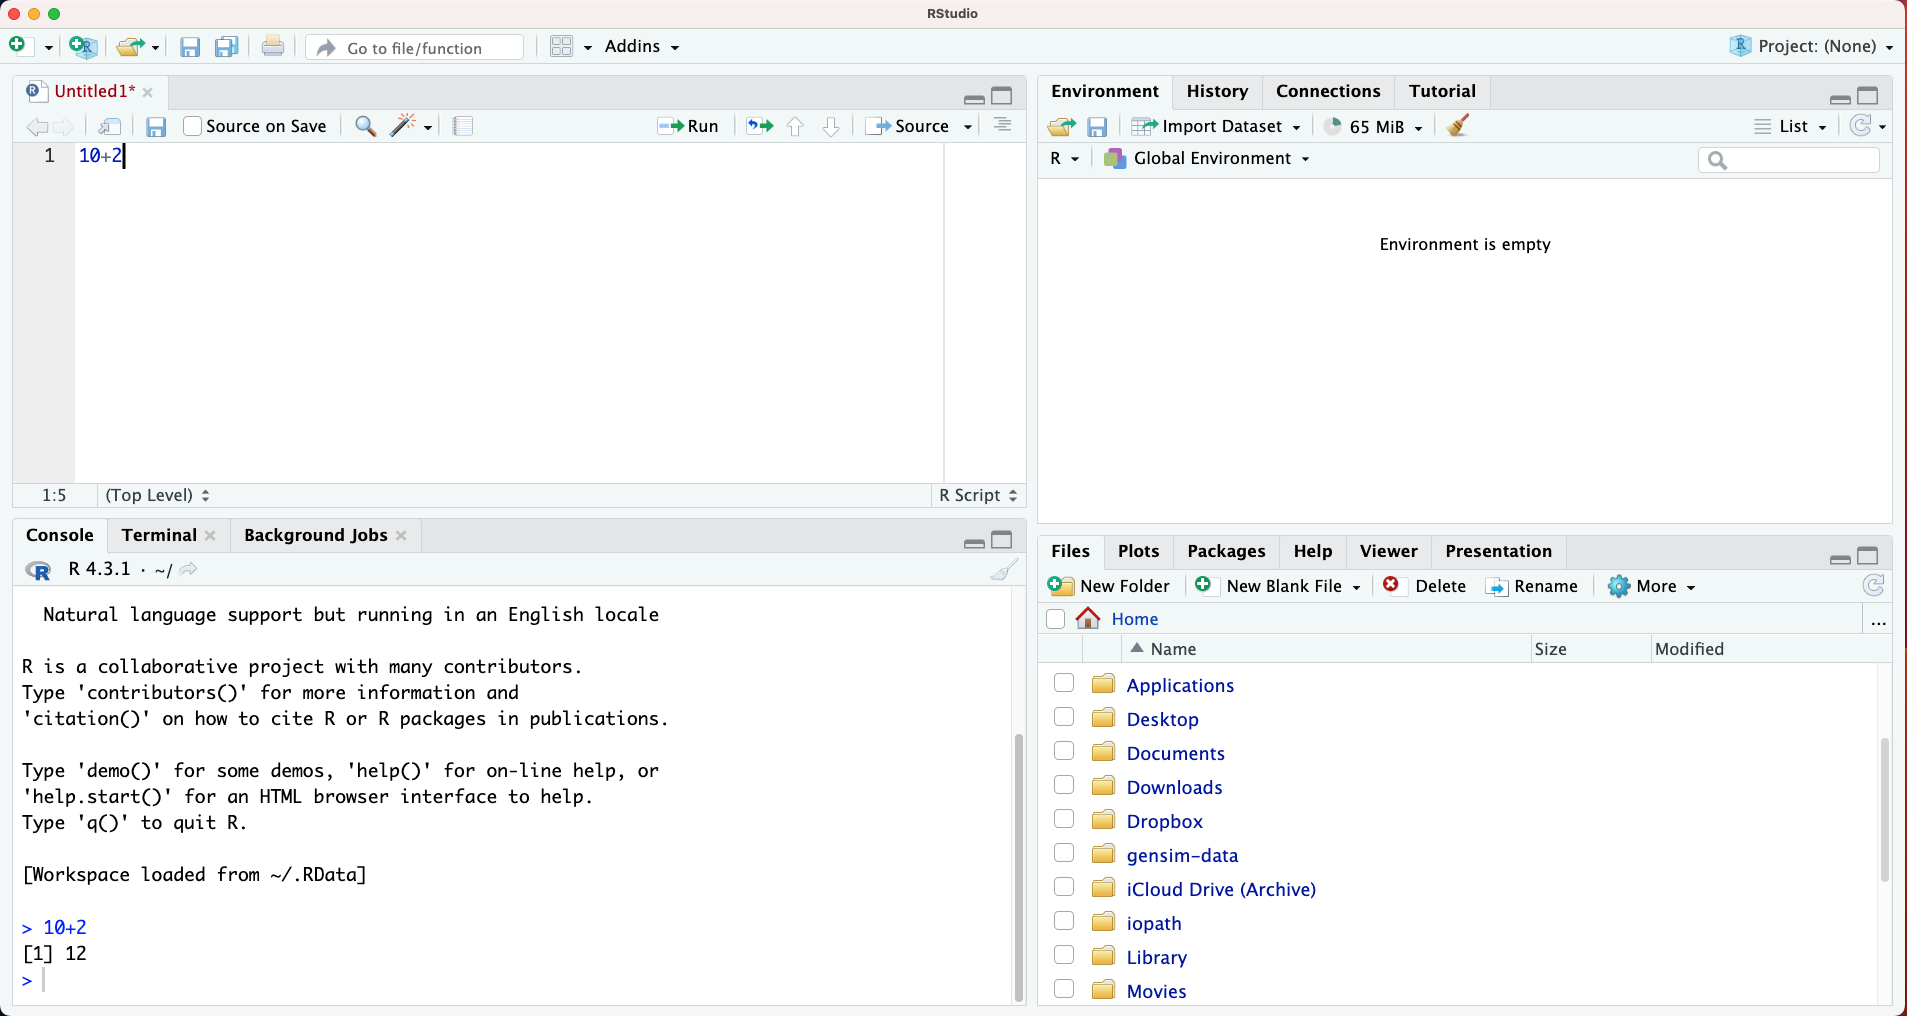
\includegraphics[width=0.9\linewidth]{images/w3_RStudio_Rfile2} \end{center}

\subsubsection*{\texorpdfstring{Open the R script \texttt{W3.R}}{Open the R script W3.R}}\label{open-the-r-script-w3.r}
\addcontentsline{toc}{subsubsection}{Open the R script \texttt{W3.R}}

The file \texttt{W3.R} can be found in the folder for this class (Quercus \textgreater{} Files \textgreater{} Practical \textgreater{} Week 3). This R script contains all the codes I will run below. You can run them on your computers as you follow along.

\section{Getting started}\label{getting-started}

\subsection*{A sophisticated calculator}\label{a-sophisticated-calculator}
\addcontentsline{toc}{subsection}{A sophisticated calculator}

\texttt{R} can do whatever your calculator can do, and much more.

\begin{Shaded}
\begin{Highlighting}[]
\DecValTok{0} \SpecialCharTok{*} \DecValTok{10}
\end{Highlighting}
\end{Shaded}

\begin{verbatim}
## [1] 0
\end{verbatim}

\begin{Shaded}
\begin{Highlighting}[]
\DecValTok{10} \SpecialCharTok{+} \DecValTok{5}
\end{Highlighting}
\end{Shaded}

\begin{verbatim}
## [1] 15
\end{verbatim}

\begin{Shaded}
\begin{Highlighting}[]
\FunctionTok{round}\NormalTok{(}\FloatTok{0.25839012}\NormalTok{,}\AttributeTok{digits=}\DecValTok{2}\NormalTok{)}
\end{Highlighting}
\end{Shaded}

\begin{verbatim}
## [1] 0.26
\end{verbatim}

\begin{Shaded}
\begin{Highlighting}[]
\FunctionTok{round}\NormalTok{(}\FloatTok{0.25839012}\NormalTok{,}\AttributeTok{digits=}\DecValTok{5}\NormalTok{)}
\end{Highlighting}
\end{Shaded}

\begin{verbatim}
## [1] 0.25839
\end{verbatim}

\subsection*{Objects}\label{objects}
\addcontentsline{toc}{subsection}{Objects}

Objects store data. You can assign objects using \texttt{\textless{}-} or \texttt{=}. In general, we use \texttt{\textless{}-} for assignment. There are distinctions between the two that are not relevant to the content here.

The way to assignment object is to type \texttt{\textless{}object\ name\textgreater{}\ \textless{}-\ \textless{}data\textgreater{}}. For example,

\begin{Shaded}
\begin{Highlighting}[]
\NormalTok{obj1 }\OtherTok{\textless{}{-}} \DecValTok{15}
\end{Highlighting}
\end{Shaded}

You will see \texttt{obj1} added to your environment panel. ``Names of objects can only contain letters, numbers, \_ (underscore), or . (period), and \emph{must begin with a letter}'' (\href{https://bookdown.org/rwnahhas/IntroToR/naming-objects.html}{An Introduction to R for Research}, emphasis added).

\subsection*{Functions}\label{functions}
\addcontentsline{toc}{subsection}{Functions}

Similar to what we did in Excel last week. Functions are what makes R useful.

Understanding a new function. Use \texttt{?\textless{}functionname\textgreater{}} to pull up the R documentation for the function. For example, one of the basic functions we need to learn is \texttt{c()} which allows you to combine data. The function \texttt{mean()} allows you to calculate the mean value, similar to the AVERAGE function we used in Microsoft Excel last week.

\begin{Shaded}
\begin{Highlighting}[]
\NormalTok{?}\FunctionTok{c}\NormalTok{()}
\NormalTok{?}\FunctionTok{mean}\NormalTok{()}
\end{Highlighting}
\end{Shaded}

We can use \texttt{c()} to combine elements, such as numbers. We can then run a function like \texttt{mean()} on the combined output.

\begin{Shaded}
\begin{Highlighting}[]
\FunctionTok{c}\NormalTok{(}\DecValTok{10}\NormalTok{,}\DecValTok{20}\NormalTok{)}
\end{Highlighting}
\end{Shaded}

\begin{verbatim}
## [1] 10 20
\end{verbatim}

We assign a new object and run \texttt{mean()} on the new object.

\begin{Shaded}
\begin{Highlighting}[]
\NormalTok{obj2 }\OtherTok{\textless{}{-}} \FunctionTok{c}\NormalTok{(}\DecValTok{10}\NormalTok{,}\DecValTok{20}\NormalTok{)}

\FunctionTok{mean}\NormalTok{(obj2)}
\end{Highlighting}
\end{Shaded}

\begin{verbatim}
## [1] 15
\end{verbatim}

\subsection*{Comments}\label{comments}
\addcontentsline{toc}{subsection}{Comments}

\texttt{R} does not evaluate lines starting with \texttt{\#}. This allow us to add glosses to our code

\begin{Shaded}
\begin{Highlighting}[]
\NormalTok{?}\FunctionTok{mean}\NormalTok{() }\CommentTok{\# this function runs R documentation for function mean()}
\end{Highlighting}
\end{Shaded}

\subsection*{Data types}\label{data-types}
\addcontentsline{toc}{subsection}{Data types}

Data types tell \texttt{R} how the object should be read. Why do they matter? They affect what calculations can be done and how functions work. Words or labels can be specified using quotations \texttt{"}. These are known as characters in R. The function \texttt{class()} will tell you what kind of data type a variable is. Now lets create two objects, one with numbers and one with characters.

\begin{Shaded}
\begin{Highlighting}[]
\NormalTok{numbers }\OtherTok{\textless{}{-}} \FunctionTok{c}\NormalTok{(}\DecValTok{10}\NormalTok{,}\DecValTok{19}\NormalTok{,}\DecValTok{100}\NormalTok{)}
\NormalTok{words }\OtherTok{\textless{}{-}} \FunctionTok{c}\NormalTok{(}\StringTok{"cat ate my homework"}\NormalTok{,}\StringTok{"today"}\NormalTok{,}\StringTok{"100 pianos"}\NormalTok{)}

\FunctionTok{class}\NormalTok{(numbers)}
\end{Highlighting}
\end{Shaded}

\begin{verbatim}
## [1] "numeric"
\end{verbatim}

\begin{Shaded}
\begin{Highlighting}[]
\FunctionTok{class}\NormalTok{(words)}
\end{Highlighting}
\end{Shaded}

\begin{verbatim}
## [1] "character"
\end{verbatim}

The exact same numbers can be read as numbers or characters. The numbers 1, 2, 3 could refer to the \texttt{numeric} type, or they could refer to the labels ``1'', ``2'', ``3'', which are the \texttt{character} type.

\begin{Shaded}
\begin{Highlighting}[]
\NormalTok{eg1 }\OtherTok{\textless{}{-}} \FunctionTok{c}\NormalTok{(}\StringTok{"1"}\NormalTok{,}\StringTok{"3"}\NormalTok{,}\StringTok{"2"}\NormalTok{)}
\FunctionTok{mean}\NormalTok{(eg1) }\CommentTok{\# characters have no mean}
\end{Highlighting}
\end{Shaded}

\begin{Shaded}
\begin{Highlighting}[]
\FunctionTok{class}\NormalTok{(eg1)}
\end{Highlighting}
\end{Shaded}

\begin{verbatim}
## [1] "character"
\end{verbatim}

There are six basic data types: character, numeric, integer, logical, complex, raw. We will only be using numeric, character, and logical types.

\subsection*{Data frames}\label{data-frames}
\addcontentsline{toc}{subsection}{Data frames}

Now, we want something closer to a dataset. We can use the column bind function \texttt{cbind()} to join two equal-length vectors. Let's create two variables

\begin{Shaded}
\begin{Highlighting}[]
\NormalTok{id }\OtherTok{\textless{}{-}} \FunctionTok{c}\NormalTok{(}\DecValTok{1}\NormalTok{,}\DecValTok{3}\NormalTok{,}\DecValTok{2}\NormalTok{) }\CommentTok{\# the first variable, let\textquotesingle{}s say we have three student ids 1,2,3}
\NormalTok{score }\OtherTok{\textless{}{-}} \FunctionTok{c}\NormalTok{(}\DecValTok{250}\NormalTok{, }\DecValTok{450}\NormalTok{, }\DecValTok{800}\NormalTok{) }\CommentTok{\# they scored 250, 450, 800 respectively}
\end{Highlighting}
\end{Shaded}

\begin{Shaded}
\begin{Highlighting}[]
\NormalTok{eg2 }\OtherTok{\textless{}{-}} \FunctionTok{cbind}\NormalTok{(id,score) }\CommentTok{\#forms a matrix with two numeric columns}
\end{Highlighting}
\end{Shaded}

View the newly created object \texttt{eg2} using \texttt{view()} function.

\begin{Shaded}
\begin{Highlighting}[]
\FunctionTok{View}\NormalTok{(eg2)}
\end{Highlighting}
\end{Shaded}

Note that using \texttt{cbind()} (column bind) function creates a matrix, which can only contain one class of data, leading to a coercion of all elements to the same class.

\begin{Shaded}
\begin{Highlighting}[]
\CommentTok{\# coercion}
\NormalTok{eg1 }\OtherTok{\textless{}{-}} \FunctionTok{cbind}\NormalTok{(}\FunctionTok{c}\NormalTok{(}\StringTok{"1"}\NormalTok{,}\DecValTok{3}\NormalTok{,}\DecValTok{2}\NormalTok{),}\FunctionTok{c}\NormalTok{(}\DecValTok{250}\NormalTok{,}\DecValTok{450}\NormalTok{,}\DecValTok{800}\NormalTok{))  }\CommentTok{\# note eg1 in your Environment is marked \textquotesingle{}chr\textquotesingle{} indication whereas eg2 is marked \textquotesingle{}num\textquotesingle{}}
\end{Highlighting}
\end{Shaded}

If we want a mix of different data types in the same table, we use the \texttt{data.frame()} function. Each variable, however, can only take be one data type. If you input a mix of character and numeric elements, they will be coerced to character for that variable, similar to the previous example above.

\begin{Shaded}
\begin{Highlighting}[]
\NormalTok{eg1 }\OtherTok{\textless{}{-}} \FunctionTok{data.frame}\NormalTok{(}\AttributeTok{v1 =} \FunctionTok{c}\NormalTok{(}\StringTok{"a"}\NormalTok{,}\StringTok{"c"}\NormalTok{,}\StringTok{"b"}\NormalTok{),}
                  \AttributeTok{v2 =} \FunctionTok{c}\NormalTok{(}\DecValTok{250}\NormalTok{,}\DecValTok{450}\NormalTok{,}\DecValTok{800}\NormalTok{)) }\CommentTok{\# notice that "=" is used here for local assignment}
\NormalTok{eg2 }\OtherTok{\textless{}{-}} \FunctionTok{data.frame}\NormalTok{(}\AttributeTok{v1 =} \FunctionTok{c}\NormalTok{(}\DecValTok{1}\NormalTok{,}\DecValTok{2}\NormalTok{,}\DecValTok{3}\NormalTok{),}
                  \AttributeTok{v2 =} \FunctionTok{c}\NormalTok{(}\DecValTok{250}\NormalTok{,}\DecValTok{800}\NormalTok{,}\DecValTok{450}\NormalTok{))}
\end{Highlighting}
\end{Shaded}

View each data frame.

\begin{Shaded}
\begin{Highlighting}[]
\FunctionTok{View}\NormalTok{(eg1)}
\FunctionTok{View}\NormalTok{(eg2)}
\end{Highlighting}
\end{Shaded}

\subsection*{Base R vs.~packages}\label{base-r-vs.-packages}
\addcontentsline{toc}{subsection}{Base R vs.~packages}

R comes with a set of base commands that allows you to do a range of statistical tasks. For example, let's try using plotting using base R functions and the object eg2.

\begin{Shaded}
\begin{Highlighting}[]
\NormalTok{?}\FunctionTok{plot}\NormalTok{() }\CommentTok{\# Generic X{-}Y Plotting}
\end{Highlighting}
\end{Shaded}

\begin{center}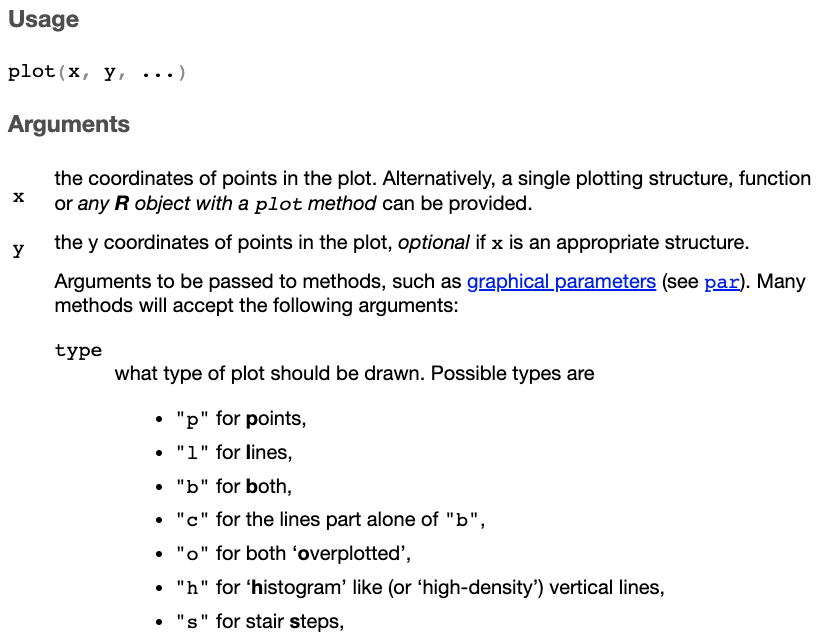
\includegraphics[width=0.7\linewidth]{images/w3_plotfunction} \end{center}

We need to specify arguments \texttt{x}, \texttt{y}, and type of plot \texttt{type}. To select one column from a dataframe, use \texttt{\$} to specify column.

\begin{Shaded}
\begin{Highlighting}[]
\FunctionTok{plot}\NormalTok{(}\AttributeTok{x =}\NormalTok{ eg2}\SpecialCharTok{$}\NormalTok{v1,}
     \AttributeTok{y =}\NormalTok{ eg2}\SpecialCharTok{$}\NormalTok{v2, }
     \AttributeTok{type =} \StringTok{"l"}\NormalTok{)}
\end{Highlighting}
\end{Shaded}

\pandocbounded{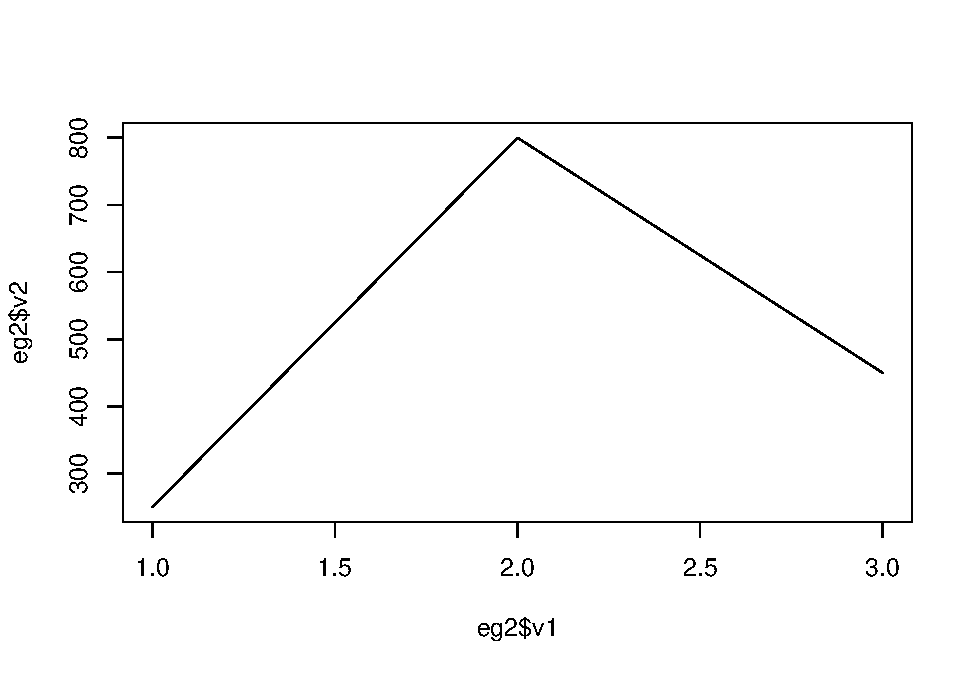
\includegraphics[keepaspectratio]{POL342-tutorial-notes_files/figure-latex/unnamed-chunk-35-1.pdf}}

\subsubsection*{Tidyverse}\label{tidyverse}
\addcontentsline{toc}{subsubsection}{Tidyverse}

R, as an open-source software, allows users to built functions using the basic functions within R. To load these additional user-built functions, we have to download and load packages. Tidyverse is a package we will be using throughout this course.

\begin{Shaded}
\begin{Highlighting}[]
\FunctionTok{install.packages}\NormalTok{(}\StringTok{"tidyverse"}\NormalTok{)}
\CommentTok{\# you only need to install packages once}
\FunctionTok{library}\NormalTok{(tidyverse) }\CommentTok{\# you have to load the package every time you restart an R session}
\end{Highlighting}
\end{Shaded}

Try using the \texttt{ggplot} function from the tidyverse package. This is complex. Don't worry if you don't understand what the code is doing. Just run it. We will be using the function repeatedly over the next few weeks.

\begin{Shaded}
\begin{Highlighting}[]
\CommentTok{\# eg1}
\FunctionTok{ggplot}\NormalTok{(}\AttributeTok{data =}\NormalTok{ eg1, }\FunctionTok{aes}\NormalTok{(}\AttributeTok{x =}\NormalTok{ v1, }\AttributeTok{y =}\NormalTok{ v2)) }\SpecialCharTok{+} \FunctionTok{geom\_line}\NormalTok{() }\CommentTok{\# eg1 is unable to plot a line because v1 is a character type}
\end{Highlighting}
\end{Shaded}

\pandocbounded{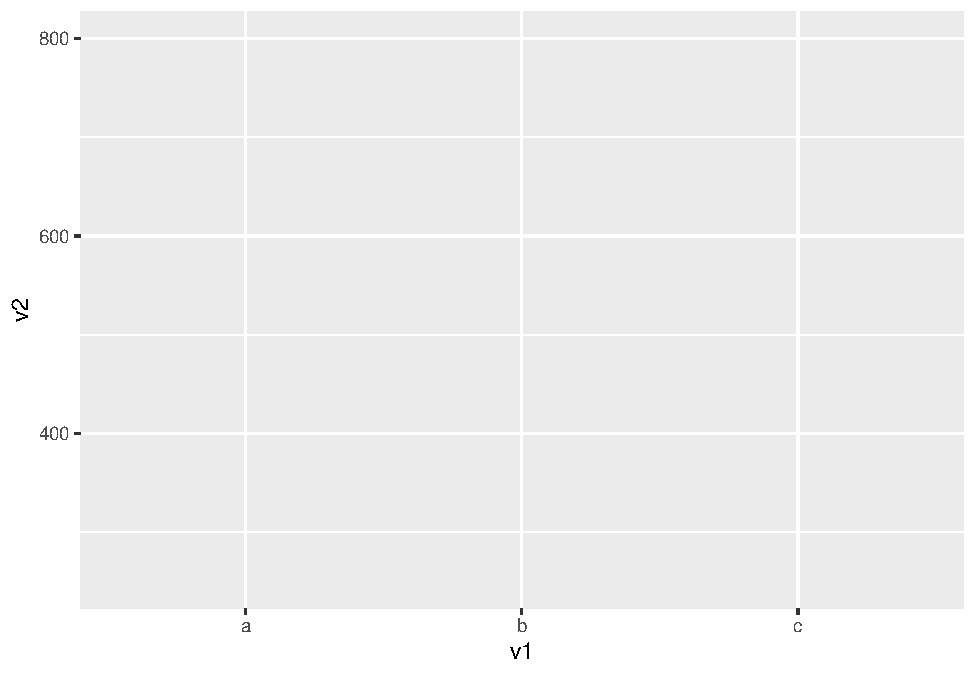
\includegraphics[keepaspectratio]{POL342-tutorial-notes_files/figure-latex/unnamed-chunk-37-1.pdf}}

\begin{Shaded}
\begin{Highlighting}[]
\CommentTok{\# eg2}
\FunctionTok{ggplot}\NormalTok{(}\AttributeTok{data =}\NormalTok{ eg2, }\FunctionTok{aes}\NormalTok{(}\AttributeTok{x =}\NormalTok{ v1, }\AttributeTok{y =}\NormalTok{ v2)) }\SpecialCharTok{+} \FunctionTok{geom\_line}\NormalTok{()}
\end{Highlighting}
\end{Shaded}

\pandocbounded{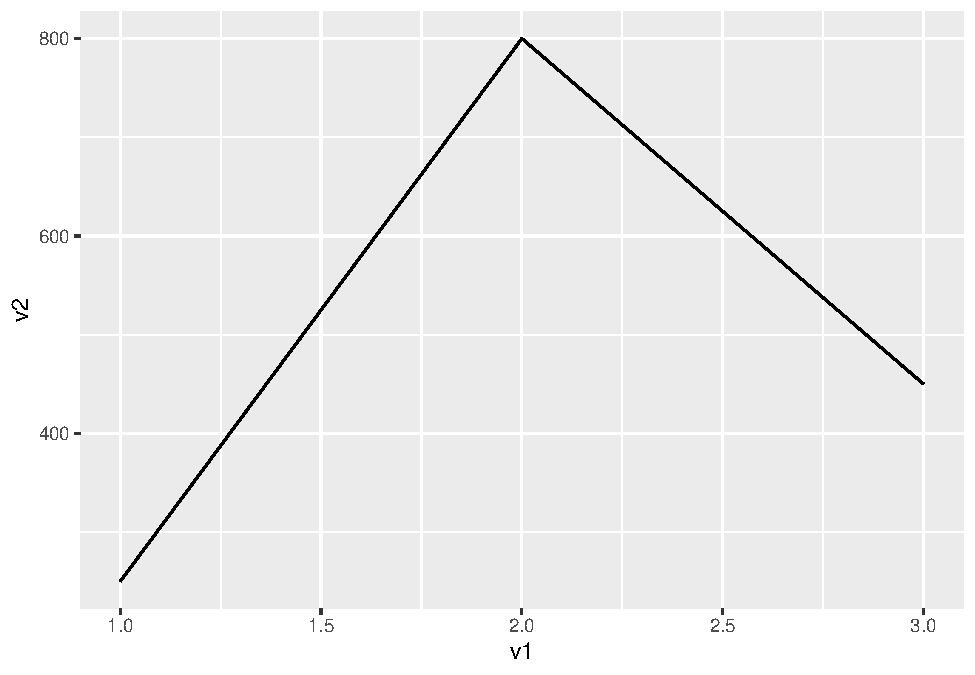
\includegraphics[keepaspectratio]{POL342-tutorial-notes_files/figure-latex/unnamed-chunk-37-2.pdf}}

\section{Working directory and importing data}\label{working-directory-and-importing-data}

You can find out your current working directory by using the function getwd(). Your working directory is the root folder where R begins to retrieve any information.

\begin{Shaded}
\begin{Highlighting}[]
\FunctionTok{getwd}\NormalTok{()}
\end{Highlighting}
\end{Shaded}

\subsubsection*{\texorpdfstring{Opening file \texttt{STAR.csv}}{Opening file STAR.csv}}\label{opening-file-star.csv}
\addcontentsline{toc}{subsubsection}{Opening file \texttt{STAR.csv}}

If the file is not in the current working directory, you can either
+ 1. Move the file to your working directory
+ 2. change your working directory (if on Mac, go to your top bar, Session \textgreater{} Set Working Directory \textgreater{} Choose Directory, and select the location where your file is located),
+ 3. alternatively, if the file is in a subfolder of your current working directory, you can retrieve it by stating the path.

We are going to use the function \texttt{read.csv()}, which takes a file path for its first argument.

\begin{Shaded}
\begin{Highlighting}[]
\CommentTok{\# the basic way to load a csv file}
\NormalTok{?}\FunctionTok{read.csv}\NormalTok{()}

\FunctionTok{paste0}\NormalTok{(}\FunctionTok{getwd}\NormalTok{(),}\StringTok{"/STAR.csv"}\NormalTok{) }\CommentTok{\# this will give you a string for the STAR.csv file if it is in your current directory}
\end{Highlighting}
\end{Shaded}

\begin{Shaded}
\begin{Highlighting}[]
\FunctionTok{read.csv}\NormalTok{(}\FunctionTok{paste0}\NormalTok{(}\FunctionTok{getwd}\NormalTok{(),}\StringTok{"/STAR.csv"}\NormalTok{)) }\CommentTok{\# this will read the file if it is in your current working directory}
\end{Highlighting}
\end{Shaded}

But that was just for illustration purposes. This can get cumbersome when dealing with multiple files.

\subsection*{R project to organize our workflow}\label{r-project-to-organize-our-workflow}
\addcontentsline{toc}{subsection}{R project to organize our workflow}

\begin{itemize}
\tightlist
\item
  \texttt{File} \textgreater{} \texttt{New\ Project...}
\item
  The location of your new project will become the default working directory. You don't have to set your working directory every time you reopen RStudio.
\end{itemize}

\begin{center}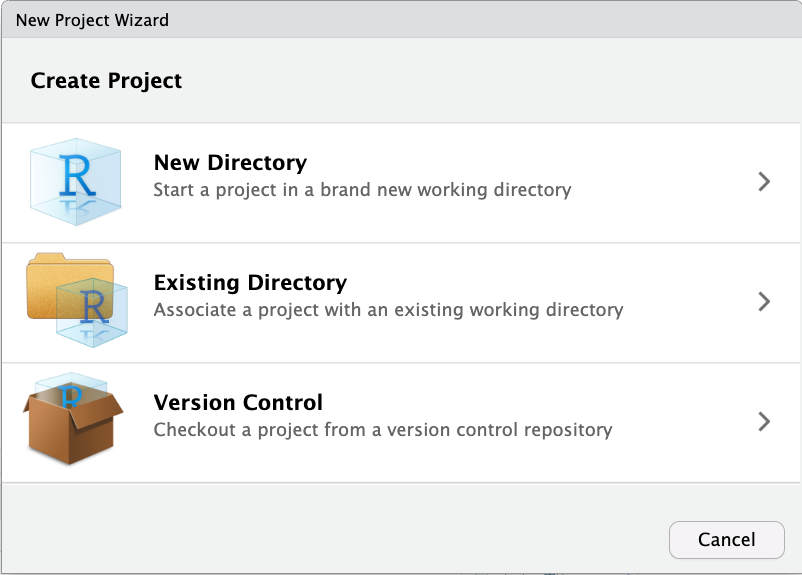
\includegraphics[width=0.7\linewidth]{images/w3_Rproj1} \end{center}

If you are not using your own laptop, save it on a portable storage, e.g.~OneDrive or your thumbdrive.

\begin{center}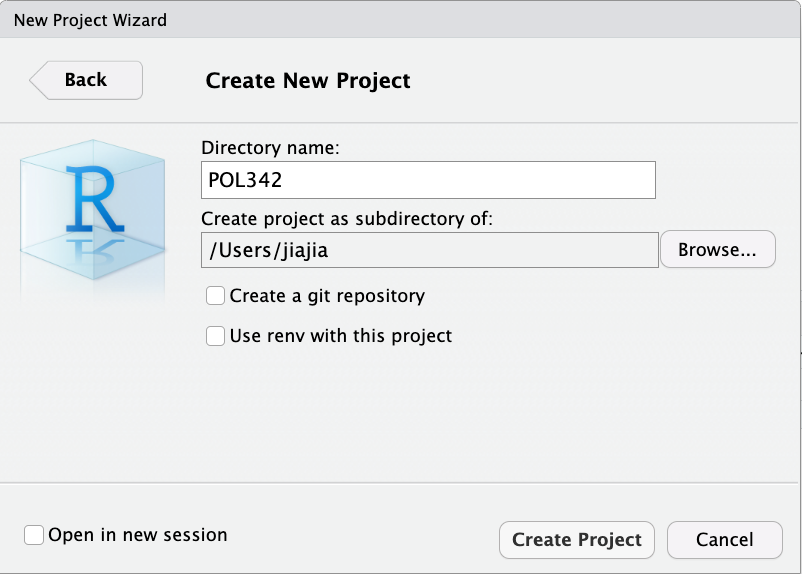
\includegraphics[width=0.7\linewidth]{images/w3_Rproj2} \end{center}

You should see a fresh view of RStudio with the project name on top.

\begin{center}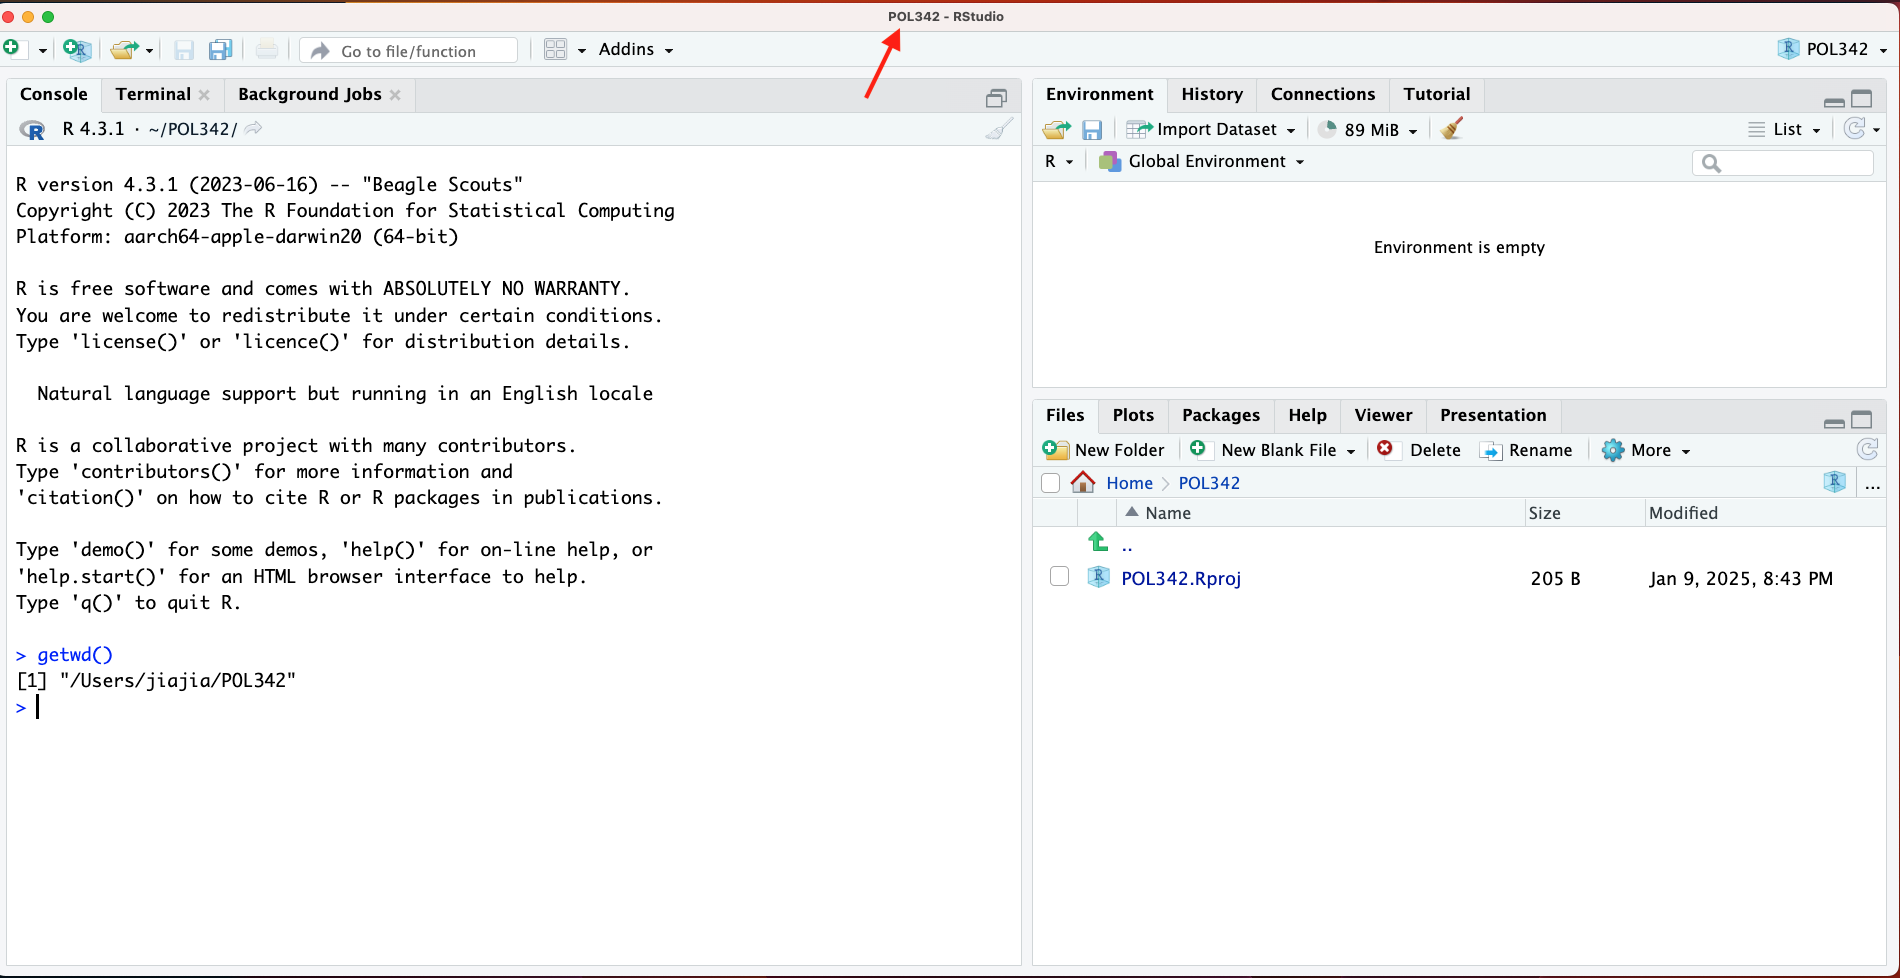
\includegraphics[width=0.7\linewidth]{images/w3_Rproj3} \end{center}

\subsubsection*{\texorpdfstring{Save \texttt{STAR.csv} in the R project folder}{Save STAR.csv in the R project folder}}\label{save-star.csv-in-the-r-project-folder}
\addcontentsline{toc}{subsubsection}{Save \texttt{STAR.csv} in the R project folder}

\begin{center}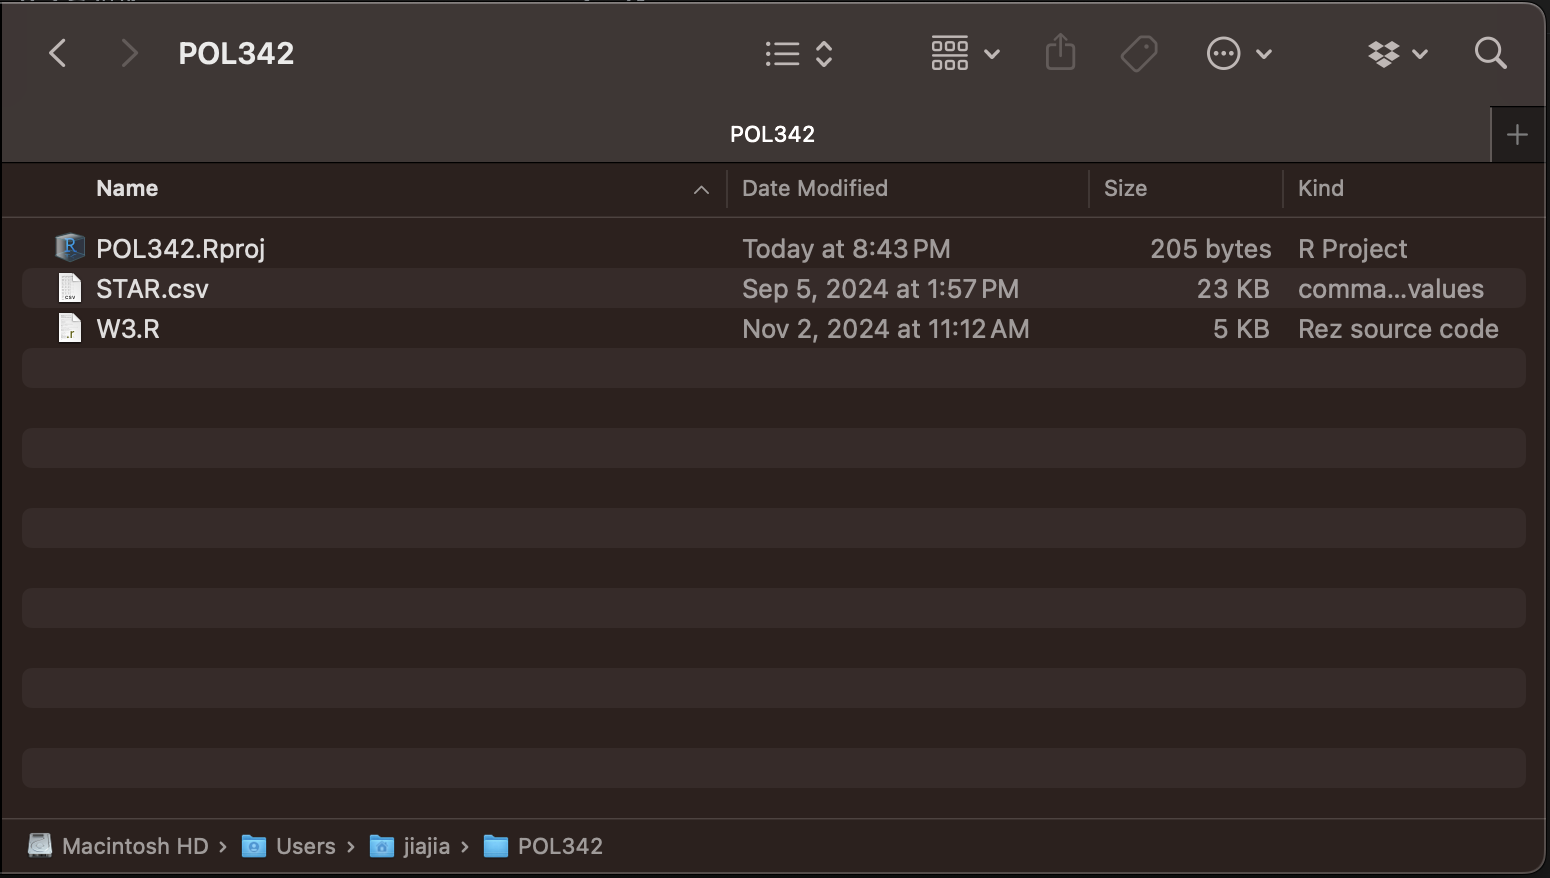
\includegraphics[width=0.7\linewidth]{images/w3_Rproj4} \end{center}

Check your file path

\begin{Shaded}
\begin{Highlighting}[]
\FunctionTok{getwd}\NormalTok{()}
\end{Highlighting}
\end{Shaded}

You should be able to run the following code if your directory matches the location of the file.

\begin{Shaded}
\begin{Highlighting}[]
\NormalTok{star }\OtherTok{\textless{}{-}} \FunctionTok{read.csv}\NormalTok{(}\StringTok{"STAR.csv"}\NormalTok{) }\CommentTok{\# reads the data file as stores it as object "star"}
\end{Highlighting}
\end{Shaded}

\subsection*{Exploring the data}\label{exploring-the-data}
\addcontentsline{toc}{subsection}{Exploring the data}

Now, we are going to do what we tried to do something similar to what we did with Microsoft Excel last week.

\begin{Shaded}
\begin{Highlighting}[]
\FunctionTok{View}\NormalTok{(star) }\CommentTok{\# look at the data}
\end{Highlighting}
\end{Shaded}

\begin{Shaded}
\begin{Highlighting}[]
\FunctionTok{head}\NormalTok{(star) }\CommentTok{\# shows the first six rows}
\end{Highlighting}
\end{Shaded}

\begin{verbatim}
##   classtype reading math graduated
## 1     small     578  610         1
## 2   regular     612  612         1
## 3   regular     583  606         1
## 4     small     661  648         1
## 5     small     614  636         1
## 6   regular     610  603         0
\end{verbatim}

\begin{itemize}
\tightlist
\item
  Identify the number of observations and names of variables
\end{itemize}

\begin{Shaded}
\begin{Highlighting}[]
\FunctionTok{dim}\NormalTok{(star) }\CommentTok{\# provides dimensions of dataframe: rows, columns}
\end{Highlighting}
\end{Shaded}

\begin{verbatim}
## [1] 1274    4
\end{verbatim}

\begin{Shaded}
\begin{Highlighting}[]
\FunctionTok{colnames}\NormalTok{(star) }\CommentTok{\# list variable names}
\end{Highlighting}
\end{Shaded}

\begin{verbatim}
## [1] "classtype" "reading"   "math"      "graduated"
\end{verbatim}

\begin{itemize}
\tightlist
\item
  Object type
\end{itemize}

\begin{Shaded}
\begin{Highlighting}[]
\FunctionTok{class}\NormalTok{(star}\SpecialCharTok{$}\NormalTok{classtype) }\CommentTok{\# column 1}
\end{Highlighting}
\end{Shaded}

\begin{verbatim}
## [1] "character"
\end{verbatim}

\begin{itemize}
\tightlist
\item
  Listing unique values for a column
\end{itemize}

\begin{Shaded}
\begin{Highlighting}[]
\FunctionTok{unique}\NormalTok{(star}\SpecialCharTok{$}\NormalTok{classtype)}
\end{Highlighting}
\end{Shaded}

\begin{verbatim}
## [1] "small"   "regular"
\end{verbatim}

\begin{itemize}
\tightlist
\item
  Calculating mean
\end{itemize}

\begin{Shaded}
\begin{Highlighting}[]
\FunctionTok{mean}\NormalTok{(star}\SpecialCharTok{$}\NormalTok{reading) }\CommentTok{\# calculates the mean of reading}
\end{Highlighting}
\end{Shaded}

\begin{verbatim}
## [1] 628.803
\end{verbatim}

\begin{Shaded}
\begin{Highlighting}[]
\FunctionTok{mean}\NormalTok{(star}\SpecialCharTok{$}\NormalTok{graduated) }\CommentTok{\# calculates the mean of graduated}
\end{Highlighting}
\end{Shaded}

\begin{verbatim}
## [1] 0.8697017
\end{verbatim}

\begin{itemize}
\tightlist
\item
  Finding mode
\item
  NOT \texttt{mode()}
\end{itemize}

\begin{Shaded}
\begin{Highlighting}[]
\FunctionTok{table}\NormalTok{(star}\SpecialCharTok{$}\NormalTok{graduated) }\CommentTok{\# tabulates all values in the column}
\end{Highlighting}
\end{Shaded}

\begin{verbatim}
## 
##    0    1 
##  166 1108
\end{verbatim}

\begin{Shaded}
\begin{Highlighting}[]
\FunctionTok{sort}\NormalTok{(}\FunctionTok{table}\NormalTok{(star}\SpecialCharTok{$}\NormalTok{graduated)) }\CommentTok{\# sorts by increasing order}
\end{Highlighting}
\end{Shaded}

\begin{verbatim}
## 
##    0    1 
##  166 1108
\end{verbatim}

\begin{itemize}
\tightlist
\item
  What if there are too many unique values?
\end{itemize}

\begin{Shaded}
\begin{Highlighting}[]
\FunctionTok{table}\NormalTok{(star}\SpecialCharTok{$}\NormalTok{reading)}
\end{Highlighting}
\end{Shaded}

\begin{verbatim}
## 
## 527 529 533 535 536 538 542 543 545 549 552 554 555 557 559 560 562 564 565 567 
##   1   3   1   1   1   1   1   1   2   3   5   4   1   6   6   2   3   5   4   4 
## 569 570 572 573 575 577 578 580 582 583 585 587 588 590 592 593 595 597 599 600 
##   4   6   5   8   4   7  14   7  15  10  13  15  15  17  16  21  24  13  12  15 
## 602 604 606 608 610 612 614 616 618 620 622 624 626 629 631 633 636 639 641 644 
##  27  20  27  27  19  20  28  31  15  21  29  27  20  50  28  39  36  27  44  29 
## 647 650 654 657 661 665 670 675 680 686 693 702 713 728 753 
##  36  49  40  34  36  37  33  31  25  26  24  17  14   9   3
\end{verbatim}

\begin{Shaded}
\begin{Highlighting}[]
\FunctionTok{sort}\NormalTok{(}\FunctionTok{table}\NormalTok{(star}\SpecialCharTok{$}\NormalTok{reading),}\AttributeTok{decreasing=}\NormalTok{T) }\CommentTok{\# sort by decreasing order}
\end{Highlighting}
\end{Shaded}

\begin{verbatim}
## 
## 629 650 641 654 633 665 636 647 661 657 670 616 675 622 644 614 631 602 606 608 
##  50  49  44  40  39  37  36  36  36  34  33  31  31  29  29  28  28  27  27  27 
## 624 639 686 680 595 693 593 620 604 612 626 610 590 702 592 582 587 588 600 618 
##  27  27  26  25  24  24  21  21  20  20  20  19  17  17  16  15  15  15  15  15 
## 578 713 585 597 599 583 728 573 577 580 557 559 570 552 564 572 554 565 567 569 
##  14  14  13  13  12  10   9   8   7   7   6   6   6   5   5   5   4   4   4   4 
## 575 529 549 562 753 545 560 527 533 535 536 538 542 543 555 
##   4   3   3   3   3   2   2   1   1   1   1   1   1   1   1
\end{verbatim}

\begin{Shaded}
\begin{Highlighting}[]
\FunctionTok{sort}\NormalTok{(}\FunctionTok{table}\NormalTok{(star}\SpecialCharTok{$}\NormalTok{reading),}\AttributeTok{decreasing=}\NormalTok{T)[}\DecValTok{1}\NormalTok{] }\CommentTok{\# limit to the first object in the table}
\end{Highlighting}
\end{Shaded}

\begin{verbatim}
## 629 
##  50
\end{verbatim}

\begin{itemize}
\tightlist
\item
  Calculating median -- two methods: median(), quantile()
\end{itemize}

\texttt{median()}

\begin{Shaded}
\begin{Highlighting}[]
\NormalTok{?}\FunctionTok{median}\NormalTok{()}

\FunctionTok{median}\NormalTok{(star}\SpecialCharTok{$}\NormalTok{reading)}
\end{Highlighting}
\end{Shaded}

\begin{verbatim}
## [1] 629
\end{verbatim}

\texttt{quantile()}

\begin{Shaded}
\begin{Highlighting}[]
\NormalTok{?quantile}

\FunctionTok{quantile}\NormalTok{(star}\SpecialCharTok{$}\NormalTok{reading, }\AttributeTok{probs=}\NormalTok{.}\DecValTok{5}\NormalTok{)}
\end{Highlighting}
\end{Shaded}

\begin{verbatim}
## 50% 
## 629
\end{verbatim}

\begin{Shaded}
\begin{Highlighting}[]
\DocumentationTok{\#\# 25th percentile, 50th percentile, 75th percentile}
\FunctionTok{quantile}\NormalTok{(star}\SpecialCharTok{$}\NormalTok{reading, }\AttributeTok{probs=}\FunctionTok{c}\NormalTok{(.}\DecValTok{25}\NormalTok{,.}\DecValTok{5}\NormalTok{,.}\DecValTok{75}\NormalTok{))}
\end{Highlighting}
\end{Shaded}

\begin{verbatim}
## 25% 50% 75% 
## 602 629 654
\end{verbatim}

\begin{itemize}
\tightlist
\item
  Standard deviation
\end{itemize}

\begin{Shaded}
\begin{Highlighting}[]
\FunctionTok{sd}\NormalTok{(star}\SpecialCharTok{$}\NormalTok{reading)}
\end{Highlighting}
\end{Shaded}

\begin{verbatim}
## [1] 36.72968
\end{verbatim}

\begin{itemize}
\tightlist
\item
  Another conveniant way to get mean and median
\end{itemize}

\begin{Shaded}
\begin{Highlighting}[]
\FunctionTok{summary}\NormalTok{(star}\SpecialCharTok{$}\NormalTok{reading)}
\end{Highlighting}
\end{Shaded}

\begin{verbatim}
##    Min. 1st Qu.  Median    Mean 3rd Qu.    Max. 
##   527.0   602.0   629.0   628.8   654.0   753.0
\end{verbatim}

When you have questions about functions and don't find the R documentations helpful, you can always turn to search engines. Most of the questions that will come up in your process of learning to use R are likely to be found on \textbf{stackoverflow}, so just search your question in Google or other search engines (and remember to indicate \texttt{R} in your searches, if not, you might get answers for other computing languages).

\section{Notes for assignment 1}\label{notes-for-assignment-1}

\subsection*{Object name}\label{object-name}
\addcontentsline{toc}{subsection}{Object name}

Object name assignment is important. If you name your data set \texttt{dat}, you should call upon the object \texttt{dat} whenever you want to use that object.

\begin{Shaded}
\begin{Highlighting}[]
\NormalTok{dat }\OtherTok{\textless{}{-}} \FunctionTok{read.csv}\NormalTok{(}\StringTok{"STAR.csv"}\NormalTok{)}

\FunctionTok{class}\NormalTok{(dat}\SpecialCharTok{$}\NormalTok{reading)}
\end{Highlighting}
\end{Shaded}

\subsection*{\texorpdfstring{Removing objects using \texttt{rm()}}{Removing objects using rm()}}\label{removing-objects-using-rm}
\addcontentsline{toc}{subsection}{Removing objects using \texttt{rm()}}

\texttt{rm()} is a function that accepts two types of arguments,

\begin{enumerate}
\def\labelenumi{\arabic{enumi}.}
\tightlist
\item
  the objects to be removed, as names (unquoted) or character strings (quoted)
\item
  list -- a character vector (or NULL) naming objects to be removed
\end{enumerate}

\subsubsection*{Method 1}\label{method-1}
\addcontentsline{toc}{subsubsection}{Method 1}

If you want to remove one object, you can use the function \texttt{rm()} and insert the object name as the argument. For example,

\begin{Shaded}
\begin{Highlighting}[]
\FunctionTok{rm}\NormalTok{(dat)}
\end{Highlighting}
\end{Shaded}

\subsubsection*{Method 2}\label{method-2}
\addcontentsline{toc}{subsubsection}{Method 2}

If your environment is cluttered and you want to clear everything in your environment without restarting the R session, you can use the function

\begin{Shaded}
\begin{Highlighting}[]
\FunctionTok{rm}\NormalTok{(}\AttributeTok{list =} \FunctionTok{ls}\NormalTok{()) }\CommentTok{\# ls() is a function that outputs all object names in the environment}
\end{Highlighting}
\end{Shaded}

\subsection*{Restarting R sessions and clearing workspace}\label{restarting-r-sessions-and-clearing-workspace}
\addcontentsline{toc}{subsection}{Restarting R sessions and clearing workspace}

When you are working on something new, you should always restart your R session and clear your workspace.

\begin{Shaded}
\begin{Highlighting}[]
\FunctionTok{rm}\NormalTok{(}\AttributeTok{list=}\FunctionTok{ls}\NormalTok{())}
\end{Highlighting}
\end{Shaded}

Start a new R session by going to Session \textgreater{} Restart R

\begin{center}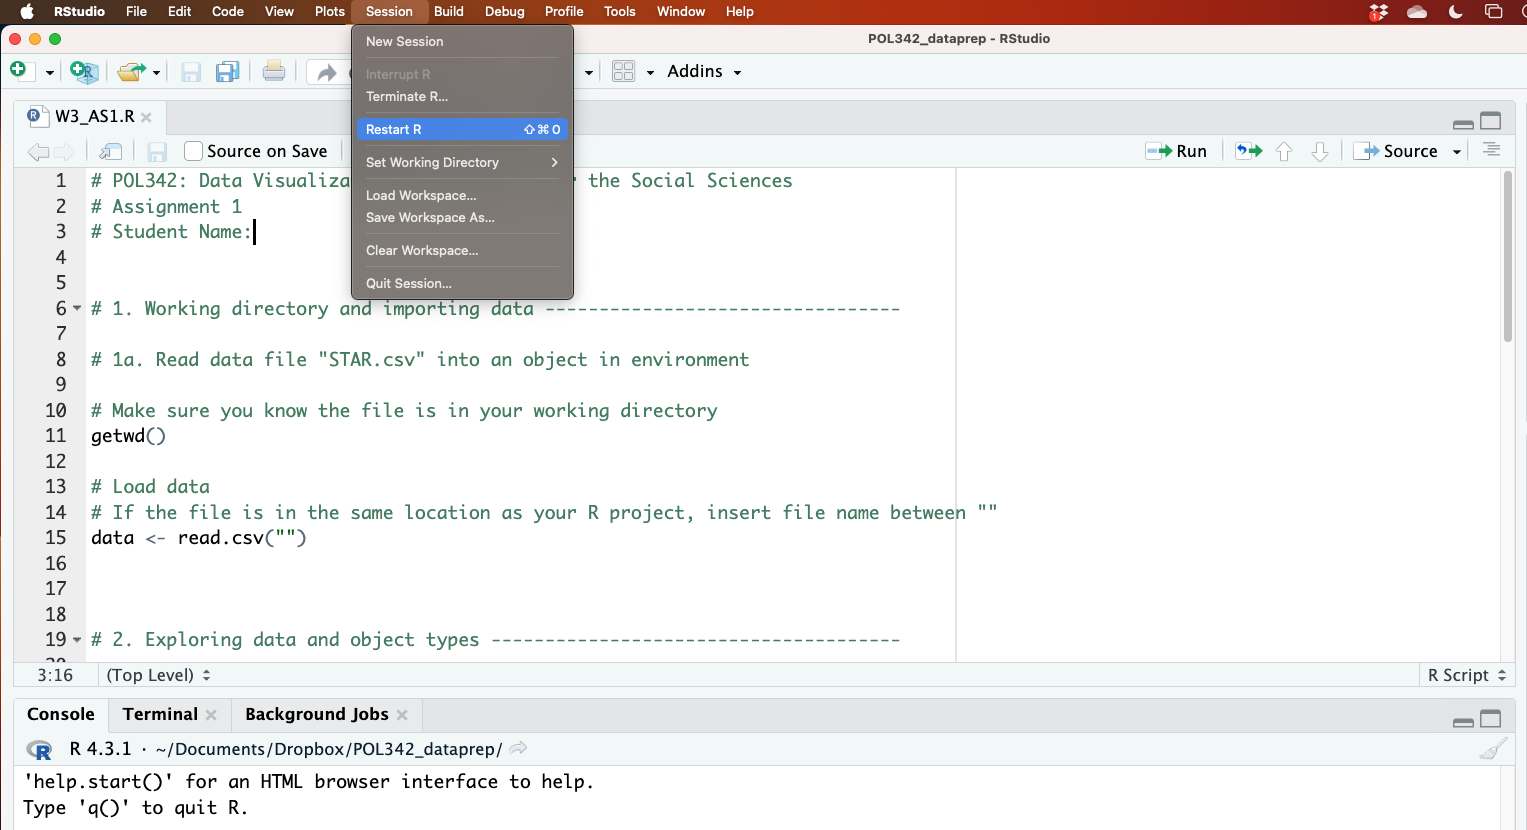
\includegraphics[width=0.7\linewidth]{images/w2_RestartR} \end{center}

Note: Depending on your default setting, restarting R session may not clear your environment. If so, you can do it by clicking on Session \textgreater{} Clear Workspace\ldots{}

\subsection*{Checking code before submission}\label{checking-code-before-submission}
\addcontentsline{toc}{subsection}{Checking code before submission}

Before submitting your code, clear your workspace and restart an R session. Then, select your entire R script and run the code. Your R script should run from beginning to end with no errors.

\section{Additional Resources}\label{additional-resources}

\begin{itemize}
\tightlist
\item
  \href{https://bookdown.org/rwnahhas/IntroToR/intro.html}{An Introduction to R for Research, chapter: Introduction}
\item
  Practise R on your own using \href{https://swirlstats.com/students.html}{Swirl: Learn R, in R}
\end{itemize}

\begin{Shaded}
\begin{Highlighting}[]
\FunctionTok{install.packages}\NormalTok{(}\StringTok{"swirl"}\NormalTok{)}
\FunctionTok{library}\NormalTok{(swirl)}
\FunctionTok{swirl}\NormalTok{()}
\end{Highlighting}
\end{Shaded}

\section{Credits}\label{credits}

\begin{itemize}
\tightlist
\item
  This lesson includes materials from

  \begin{itemize}
  \tightlist
  \item
    \href{https://scholar.harvard.edu/ellaudet/DSS}{Data Analysis for Social Science}
  \item
    \href{https://moderndive.com/index.html}{Statistical Inference via Data Science: A ModernDive into R and the Tidyverse}
  \end{itemize}
\end{itemize}

\chapter{Data Wrangling with Tidyverse}\label{data-wrangling-with-tidyverse}

Goals for today's class:

\begin{itemize}
\tightlist
\item
  Tidyverse basics for datasets

  \begin{itemize}
  \tightlist
  \item
    \texttt{filter()}
  \item
    \texttt{reframe()}
  \item
    \texttt{group\_by()}
  \item
    \texttt{mutate()}
  \item
    \texttt{arrange()}
  \item
    \texttt{select()}
  \end{itemize}
\end{itemize}

\section{Before the start of each class}\label{before-the-start-of-each-class}

You should download the \texttt{.R} script and dataset from the Quercus folder for this week (Files \textgreater{} Practical \textgreater{} Week 4). Move the files to the .R project folder we created last week. Your folder should look something like this now:

\begin{center}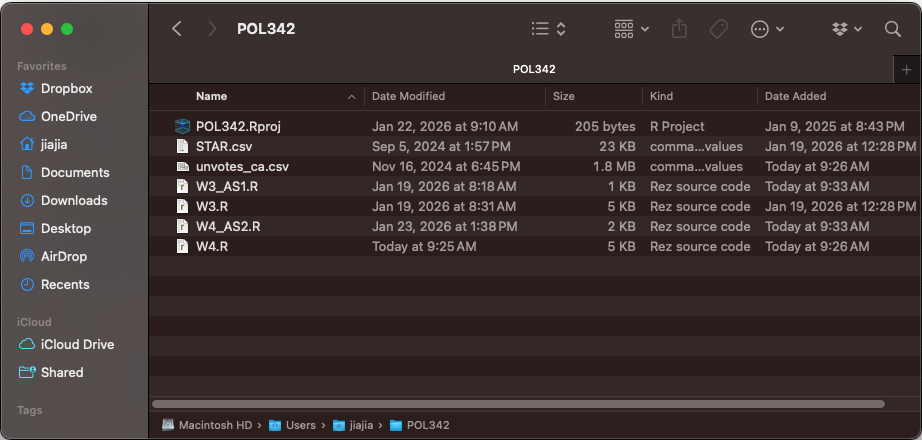
\includegraphics[width=0.8\linewidth]{images/w4_Rprojectfolder} \end{center}

Open RStudio using your \texttt{.Rproject} file and follow along using the \texttt{W4.R} script.

\begin{center}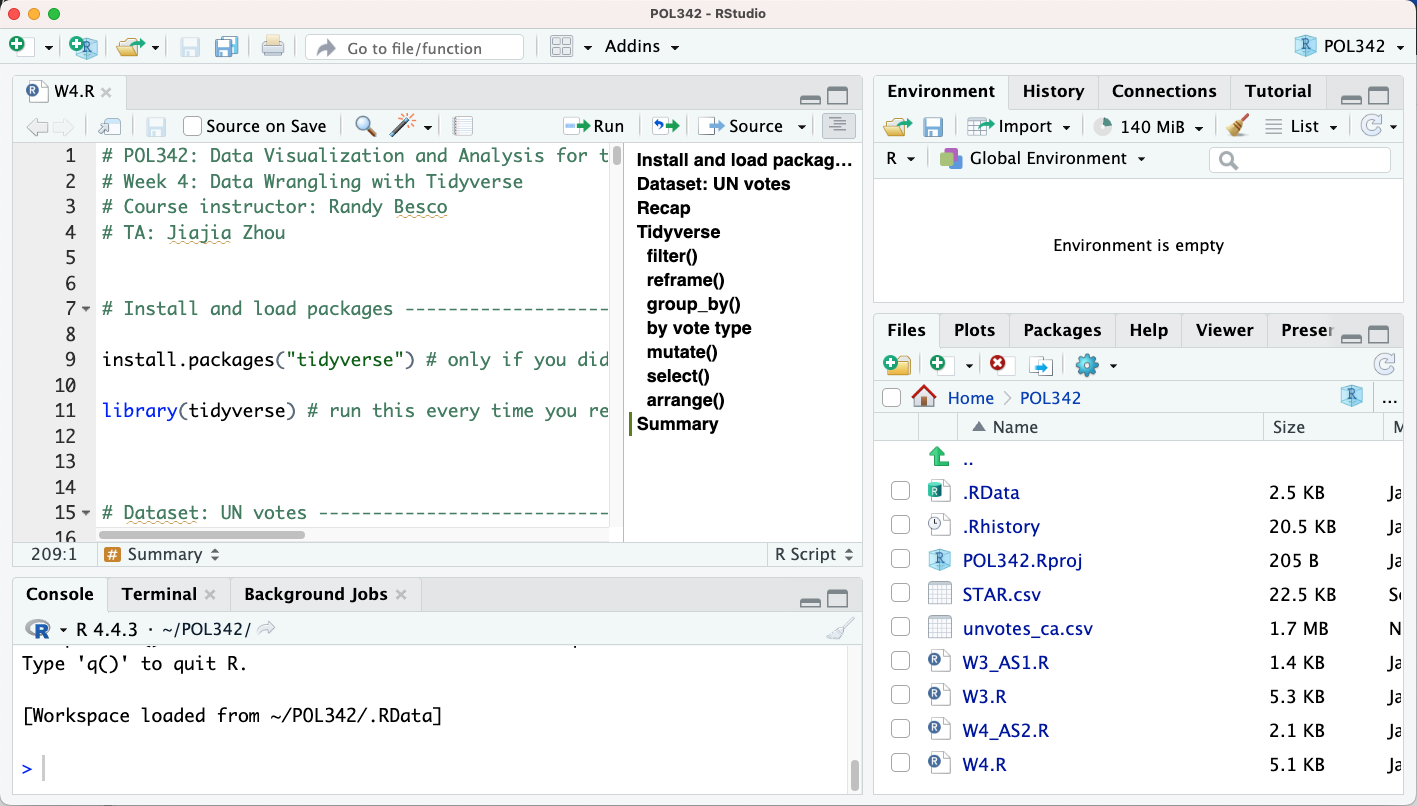
\includegraphics[width=0.8\linewidth]{images/w4_RstudioSetup} \end{center}

\section{Install and load packages}\label{install-and-load-packages}

\begin{Shaded}
\begin{Highlighting}[]
\FunctionTok{install.packages}\NormalTok{(}\StringTok{"tidyverse"}\NormalTok{) }\CommentTok{\# if you haven\textquotesingle{}t}

\FunctionTok{library}\NormalTok{(tidyverse)}
\end{Highlighting}
\end{Shaded}

\section{Dataset: UN votes}\label{dataset-un-votes}

The data for UN votes here come from the package ``unvotes.'' You can find out more about the package here: \url{https://github.com/dgrtwo/unvotes} and\\
\url{https://cran.r-project.org/web/packages/unvotes/unvotes.pdf}

Know your current directory and where the data file is. You should be using the R project you created last week.

\begin{Shaded}
\begin{Highlighting}[]
\FunctionTok{getwd}\NormalTok{() }\CommentTok{\#run to display working directory}
\end{Highlighting}
\end{Shaded}

\subsection*{\texorpdfstring{Read file as \texttt{unvotes} data.frame object}{Read file as unvotes data.frame object}}\label{read-file-as-unvotes-data.frame-object}
\addcontentsline{toc}{subsection}{Read file as \texttt{unvotes} data.frame object}

The following code will work if you have \texttt{unvotes\_ca.csv} file in your R project folder.

\begin{Shaded}
\begin{Highlighting}[]
\NormalTok{unvotes }\OtherTok{\textless{}{-}} \FunctionTok{read.csv}\NormalTok{(}\StringTok{"unvotes\_ca.csv"}\NormalTok{)}
\end{Highlighting}
\end{Shaded}

\begin{longtable}[]{@{}
  >{\raggedright\arraybackslash}p{(\linewidth - 2\tabcolsep) * \real{0.0968}}
  >{\raggedright\arraybackslash}p{(\linewidth - 2\tabcolsep) * \real{0.9032}}@{}}
\toprule\noalign{}
\begin{minipage}[b]{\linewidth}\raggedright
variable
\end{minipage} & \begin{minipage}[b]{\linewidth}\raggedright
desc.
\end{minipage} \\
\midrule\noalign{}
\endhead
\bottomrule\noalign{}
\endlastfoot
rcid & The roll call id; used to join with un\_votes and un\_roll\_call\_issues \\
country & Country name, by official English short name \\
country\_code & 2-character ISO country code \\
year & Year in which vote took place \\
vote & Vote result as a factor of yes/abstain/no \\
session & Session number. The UN holds one session per year; these started in 1946 \\
importantvote & Whether the vote was classified as important by the U.S. State Department report ``Voting Practices in the United Nations''. These classifications began with session 39 \\
date & Date of the vote, as a Date vector \\
unres & Resolution code \\
amend & Whether the vote was on an amendment; coded only until 1985 \\
para & Whether the vote was only on a paragraph and not a resolution; coded only until 1985 \\
short & Short description \\
descr & Longer description \\
short\_name & Two-letter issue codes \\
issue & Descriptive issue name \\
\end{longtable}

\subsection*{View the data}\label{view-the-data}
\addcontentsline{toc}{subsection}{View the data}

\begin{Shaded}
\begin{Highlighting}[]
\FunctionTok{View}\NormalTok{(unvotes)}

\CommentTok{\# or display first few rows of the data}
\FunctionTok{head}\NormalTok{(unvotes,}\DecValTok{5}\NormalTok{)}
\end{Highlighting}
\end{Shaded}

\begin{verbatim}
##   rcid country country_code year vote session importantvote       date   unres
## 1    6  Canada           CA 1946   no       1             0 1946-01-04 R/1/107
## 2    8  Canada           CA 1946  yes       1             0 1946-01-05 R/1/297
## 3   11  Canada           CA 1946  yes       1             0 1946-02-05 R/1/376
## 4   11  Canada           CA 1946  yes       1             0 1946-02-05 R/1/376
## 5   18  Canada           CA 1946   no       1             0 1946-02-03 R/1/532
##   amend para                       short
## 1     0    0 DECLARATION OF HUMAN RIGHTS
## 2     1    0               ECOSOC POWERS
## 3     0    0      TRUSTEESHIP AMENDMENTS
## 4     0    0      TRUSTEESHIP AMENDMENTS
## 5     1    0          ECOSOC CONSULTANTS
##                                                                                                                                                                                                                                                   descr
## 1                                                                                                                                            TO ADOPT A CUBAN PROPOSAL (A/3-C) THAT AN ITEM ON A DECLARATION OF THE RIGHTS AND DUTIES OF MAN BE TABLED.
## 2  TO ADOPT A SECOND 6TH COMM. AMENDMENT (A/14) TO THE PROVISIONAL RULES OF PROCEDURE, WHICH AMENDMENT EPLACES PROVISIONAL RULE T WITH A NEW TEXT AUTHORIZING THE ECONOMIC & SOC. COUNCIL TO CALL INTERNATIONAL CONFERENCES ON ANY MATTER WITHIN ITS CO
## 3  TO ADOPT DRAFT RESOLUTIONS I AND II AS A WHOLE, OF THE 4TH COMM. REPORT (A/34) ON NON-SELF-GOVERNING TERRITORIES. RESOLUTION I PROVIDES TO PROMOTE THE POLITICAL, SOCIAL, ECONOMIC, AND EDUCATIONAL ASPIRATIONS OF NON-SELF-GOVERNING PEOPLES THROUG
## 4  TO ADOPT DRAFT RESOLUTIONS I AND II AS A WHOLE, OF THE 4TH COMM. REPORT (A/34) ON NON-SELF-GOVERNING TERRITORIES. RESOLUTION I PROVIDES TO PROMOTE THE POLITICAL, SOCIAL, ECONOMIC, AND EDUCATIONAL ASPIRATIONS OF NON-SELF-GOVERNING PEOPLES THROUG
## 5 TO ADOPT USSR (ORAL) AMENDMENT REPLACING THE 1ST COMM. DRAFT RESOLUTION (A/54/REV.1) WITH THE FOLLOWING:  \\TAKING INTO CONSIDERATION THE QUESTION RAISED BY THE WORLD FEDERATION OF TRADE UNIONS CONCERNING ITS PARTICIPATION IN THE WORK OF THE ECO
##   short_name                issue
## 1         hr         Human rights
## 2         ec Economic development
## 3         co          Colonialism
## 4         ec Economic development
## 5         ec Economic development
\end{verbatim}

\section{Recap}\label{recap}

We are going to spend around 15-30 minutes practising what we learnt last week.

\begin{itemize}
\tightlist
\item
  Try answering the following questions based on what we learnt last week:

  \begin{itemize}
  \tightlist
  \item
    What are the names of the 15 variables in the dataset? (Hint: \texttt{colnames()})
  \item
    What are the data types of variables \texttt{vote} and \texttt{issue}? (Hint: \texttt{class()})
  \item
    What are the unique values in \texttt{vote} and \texttt{issue}? (Hint: \texttt{unique()})
  \item
    Could you provide a tally of the data under \texttt{vote}? (Hint: \texttt{table()})
  \item
    What is the median \texttt{year} in the dataset?
  \end{itemize}
\end{itemize}

\section{Tidyverse}\label{tidyverse-1}

\subsection*{Pipes}\label{pipes}
\addcontentsline{toc}{subsection}{Pipes}

Two types of piping \texttt{\textbar{}\textgreater{}} (base R) and \texttt{\%\textgreater{}\%} (magrittr). The differences are not meaningful for this course. We will be using the \texttt{\textbar{}\textgreater{}} pipe for simplicity.

Tidyverse pipes facilitate a sequence of actions performed on \textbf{a single object}. After every action, the \texttt{\textbar{}\textgreater{}} is used to indicate that the output of the previous action is used as the input of the next action.

To make sure the pipe runs, the function must be able to take the piped object as its first argument.

\begin{Shaded}
\begin{Highlighting}[]
\DocumentationTok{\#\# the following codes are equivalent}
\CommentTok{\#Base R}
\FunctionTok{summary}\NormalTok{(unvotes)}
\end{Highlighting}
\end{Shaded}

\begin{verbatim}
##       rcid        country          country_code            year     
##  Min.   :   6   Length:5732        Length:5732        Min.   :1946  
##  1st Qu.:2100   Class :character   Class :character   1st Qu.:1979  
##  Median :3540   Mode  :character   Mode  :character   Median :1990  
##  Mean   :3491                                         Mean   :1991  
##  3rd Qu.:4797                                         3rd Qu.:2006  
##  Max.   :9145                                         Max.   :2019  
##                                                                     
##      vote              session      importantvote         date          
##  Length:5732        Min.   : 1.00   Min.   :0.00000   Length:5732       
##  Class :character   1st Qu.:34.00   1st Qu.:0.00000   Class :character  
##  Mode  :character   Median :45.00   Median :0.00000   Mode  :character  
##                     Mean   :45.65   Mean   :0.08442                     
##                     3rd Qu.:61.00   3rd Qu.:0.00000                     
##                     Max.   :74.00   Max.   :1.00000                     
##                                     NA's   :425                         
##     unres               amend             para           short          
##  Length:5732        Min.   :0.0000   Min.   :0.0000   Length:5732       
##  Class :character   1st Qu.:0.0000   1st Qu.:0.0000   Class :character  
##  Mode  :character   Median :0.0000   Median :0.0000   Mode  :character  
##                     Mean   :0.0486   Mean   :0.2365                     
##                     3rd Qu.:0.0000   3rd Qu.:0.0000                     
##                     Max.   :1.0000   Max.   :1.0000                     
##                     NA's   :3553     NA's   :3330                       
##     descr            short_name           issue          
##  Length:5732        Length:5732        Length:5732       
##  Class :character   Class :character   Class :character  
##  Mode  :character   Mode  :character   Mode  :character  
##                                                          
##                                                          
##                                                          
## 
\end{verbatim}

\begin{Shaded}
\begin{Highlighting}[]
\CommentTok{\#Tidyverse}
\NormalTok{unvotes }\SpecialCharTok{|\textgreater{}} \FunctionTok{summary}\NormalTok{()}
\end{Highlighting}
\end{Shaded}

\begin{verbatim}
##       rcid        country          country_code            year     
##  Min.   :   6   Length:5732        Length:5732        Min.   :1946  
##  1st Qu.:2100   Class :character   Class :character   1st Qu.:1979  
##  Median :3540   Mode  :character   Mode  :character   Median :1990  
##  Mean   :3491                                         Mean   :1991  
##  3rd Qu.:4797                                         3rd Qu.:2006  
##  Max.   :9145                                         Max.   :2019  
##                                                                     
##      vote              session      importantvote         date          
##  Length:5732        Min.   : 1.00   Min.   :0.00000   Length:5732       
##  Class :character   1st Qu.:34.00   1st Qu.:0.00000   Class :character  
##  Mode  :character   Median :45.00   Median :0.00000   Mode  :character  
##                     Mean   :45.65   Mean   :0.08442                     
##                     3rd Qu.:61.00   3rd Qu.:0.00000                     
##                     Max.   :74.00   Max.   :1.00000                     
##                                     NA's   :425                         
##     unres               amend             para           short          
##  Length:5732        Min.   :0.0000   Min.   :0.0000   Length:5732       
##  Class :character   1st Qu.:0.0000   1st Qu.:0.0000   Class :character  
##  Mode  :character   Median :0.0000   Median :0.0000   Mode  :character  
##                     Mean   :0.0486   Mean   :0.2365                     
##                     3rd Qu.:0.0000   3rd Qu.:0.0000                     
##                     Max.   :1.0000   Max.   :1.0000                     
##                     NA's   :3553     NA's   :3330                       
##     descr            short_name           issue          
##  Length:5732        Length:5732        Length:5732       
##  Class :character   Class :character   Class :character  
##  Mode  :character   Mode  :character   Mode  :character  
##                                                          
##                                                          
##                                                          
## 
\end{verbatim}

\subsection*{Piping data frames}\label{piping-data-frames}
\addcontentsline{toc}{subsection}{Piping data frames}

In this course, our focus is on data sets (i.e.~data frames). Hence for the rest of today's class, we will focus on six tidyverse functions that are developed for the purpose of manipulating data frames.

\begin{itemize}
\tightlist
\item
  Tidyverse functions for datasets

  \begin{itemize}
  \tightlist
  \item
    \texttt{filter()} : subsets the data based on a conditional statement
  \item
    \texttt{reframe()} : collapses/summarizes the dataset to produce stated summary statistics (e.g.~\texttt{mean()})
  \item
    \texttt{group\_by()} : divides the data based on specified groups so that subsequent functions can be run on each group separately
  \item
    \texttt{mutate()} : creates a new variable (i.e.~new column) in the dataset
  \item
    \texttt{arrange()} : order the rows based on a criterion
  \item
    \texttt{select()} : keep columns using their variable names (columns not specified are dropped from the dataset)
  \end{itemize}
\end{itemize}

\subsection*{filter()}\label{filter}
\addcontentsline{toc}{subsection}{filter()}

The \texttt{filter()} function allows you to slice out parts of the data based on your criterion.

\begin{Shaded}
\begin{Highlighting}[]
\CommentTok{\# Subset only rows in the 60th UNGA session and save as new object}
\NormalTok{unvotes }\SpecialCharTok{|\textgreater{}} 
  \FunctionTok{filter}\NormalTok{(session}\SpecialCharTok{==}\DecValTok{60}\NormalTok{)}
\end{Highlighting}
\end{Shaded}

\begin{Shaded}
\begin{Highlighting}[]
\NormalTok{sess60 }\OtherTok{\textless{}{-}}\NormalTok{ unvotes }\SpecialCharTok{|\textgreater{}} 
  \FunctionTok{filter}\NormalTok{(session}\SpecialCharTok{==}\DecValTok{60}\NormalTok{)}

\CommentTok{\# top 8 rows in the session 60 subset}
\FunctionTok{head}\NormalTok{(sess60,}\DecValTok{8}\NormalTok{)}
\end{Highlighting}
\end{Shaded}

\begin{verbatim}
##   rcid country country_code year    vote session importantvote       date
## 1 4593  Canada           CA 2006     yes      60             0 2006-03-15
## 2 4594  Canada           CA 2005     yes      60             0 2005-12-23
## 3 4599  Canada           CA 2005 abstain      60             1 2005-12-22
## 4 4600  Canada           CA 2005 abstain      60             1 2005-12-22
## 5 4601  Canada           CA 2005     yes      60             0 2005-12-22
## 6 4602  Canada           CA 2005     yes      60             0 2005-12-16
## 7 4603  Canada           CA 2005     yes      60             0 2005-12-16
## 8 4604  Canada           CA 2005     yes      60             0 2005-12-16
##      unres amend para
## 1 R/60/251    NA   NA
## 2 R/60/231    NA   NA
## 3 R/60/185    NA   NA
## 4 R/60/184    NA   NA
## 5 R/60/183    NA   NA
## 6 R/60/170    NA   NA
## 7 R/60/174    NA   NA
## 8 R/60/173    NA   NA
##                                                               short
## 1      Human Rights Council : resolution / adopted by the General A
## 2      Rights of the child : resolution / adopted by the General As
## 3      Unilateral economic measures as a means of political and eco
## 4      International trade and development : resolution / adopted b
## 5      Permanent sovereignty of the Palestinian people in the Occup
## 6       Situation of human rights in the Democratic Republic of the
## 7      Situation of human rights in Uzbekistan : resolution / adopt
## 8 Situation of human rights in the Democratic People?Æs Republi
##                                                                                                                                                                                                                                                  descr
## 1                                                                                                                                                                                  Human Rights Council : resolution / adopted by the General Assembly
## 2                                                                                                                                                                                   Rights of the child : resolution / adopted by the General Assembly
## 3                                                                                               Unilateral economic measures as a means of political and economic coercion against developing countries : resolution / adopted by the General Assembly
## 4                                                                                                                                                                   International trade and development : resolution / adopted by the General Assembly
## 5 Permanent sovereignty of the Palestinian people in the Occupied Palestinian Territory, including East Jerusalem, and of the Arab population in the occupied Syrian Golan over their natural resources : resolution / adopted by the General Assembly
## 6                                                                                                                                     Situation of human rights in the Democratic Republic of the Congo : resolution / adopted by the General Assembly
## 7                                                                                                                                                               Situation of human rights in Uzbekistan : resolution / adopted by the General Assembly
## 8                                                                                                                              Situation of human rights in the Democratic People?Æs Republic of Korea : resolution / adopted by the General Assembly
##   short_name                issue
## 1         hr         Human rights
## 2         hr         Human rights
## 3         ec Economic development
## 4         ec Economic development
## 5         me Palestinian conflict
## 6         hr         Human rights
## 7         hr         Human rights
## 8         hr         Human rights
\end{verbatim}

To understand how to \texttt{filter} datasets based on a certain criterion, we need to understand how to construct conditional statements using operators.

\subsubsection*{Conditional statements and operators}\label{conditional-statements-and-operators}
\addcontentsline{toc}{subsubsection}{Conditional statements and operators}

Conditional statements produce \texttt{logical} class (i.e.~TRUE or FALSE) output that help us to manipulate objects as well as customize the execution of functions.

Operators are used to construct conditional statements.

\begin{itemize}
\tightlist
\item
  Comparison operators

  \begin{itemize}
  \tightlist
  \item
    Equal \texttt{==}
  \item
    Not equal \texttt{!=}
  \item
    More than \texttt{\textgreater{}}
  \item
    Less than \texttt{\textless{}}
  \item
    Greater than or equal to \texttt{\textgreater{}=}
  \item
    Less than or equal to \texttt{\textless{}=}
  \end{itemize}
\item
  Logical operators

  \begin{itemize}
  \tightlist
  \item
    And \texttt{\&}
  \item
    Or \texttt{\textbar{}}
  \item
    Not \texttt{!}
  \end{itemize}
\item
  Miscellaneous operator

  \begin{itemize}
  \tightlist
  \item
    In \texttt{\%in\%}
  \end{itemize}
\end{itemize}

\subsubsection*{Run a few examples to see how they work}\label{run-a-few-examples-to-see-how-they-work}
\addcontentsline{toc}{subsubsection}{Run a few examples to see how they work}

\begin{itemize}
\tightlist
\item
  5 MORE THAN 3
\end{itemize}

\begin{Shaded}
\begin{Highlighting}[]
\DecValTok{5} \SpecialCharTok{\textgreater{}} \DecValTok{3}
\end{Highlighting}
\end{Shaded}

\begin{verbatim}
## [1] TRUE
\end{verbatim}

\begin{itemize}
\tightlist
\item
  10 LESS THAN -100
\end{itemize}

\begin{Shaded}
\begin{Highlighting}[]
\DecValTok{10} \SpecialCharTok{\textless{}} \SpecialCharTok{{-}}\DecValTok{100}
\end{Highlighting}
\end{Shaded}

\begin{verbatim}
## [1] FALSE
\end{verbatim}

\begin{itemize}
\tightlist
\item
  ``3 more than 5'' AND ``3 more than 1''
\end{itemize}

\begin{Shaded}
\begin{Highlighting}[]
\NormalTok{(}\DecValTok{3} \SpecialCharTok{\textgreater{}} \DecValTok{5}\NormalTok{) }\SpecialCharTok{\&}\NormalTok{ (}\DecValTok{3} \SpecialCharTok{\textgreater{}} \DecValTok{1}\NormalTok{)}
\end{Highlighting}
\end{Shaded}

\begin{verbatim}
## [1] FALSE
\end{verbatim}

\begin{itemize}
\tightlist
\item
  ``3 more than 5'' OR ``3 more than 1''
\end{itemize}

\begin{Shaded}
\begin{Highlighting}[]
\NormalTok{(}\DecValTok{3} \SpecialCharTok{\textgreater{}} \DecValTok{5}\NormalTok{) }\SpecialCharTok{|}\NormalTok{ (}\DecValTok{3} \SpecialCharTok{\textgreater{}} \DecValTok{1}\NormalTok{)}
\end{Highlighting}
\end{Shaded}

\begin{verbatim}
## [1] TRUE
\end{verbatim}

\begin{itemize}
\tightlist
\item
  1 EQUALS TO 3
\end{itemize}

\begin{Shaded}
\begin{Highlighting}[]
\DecValTok{1} \SpecialCharTok{==} \DecValTok{3}
\end{Highlighting}
\end{Shaded}

\begin{verbatim}
## [1] FALSE
\end{verbatim}

\begin{itemize}
\tightlist
\item
  ``apple'' EQUALS TO ``apple''
\end{itemize}

\begin{Shaded}
\begin{Highlighting}[]
\NormalTok{eg }\OtherTok{\textless{}{-}} \StringTok{"apple"}
\NormalTok{eg2 }\OtherTok{\textless{}{-}} \StringTok{"banana"}

\NormalTok{eg }\SpecialCharTok{==} \StringTok{"apple"}
\end{Highlighting}
\end{Shaded}

\begin{verbatim}
## [1] TRUE
\end{verbatim}

\begin{Shaded}
\begin{Highlighting}[]
\NormalTok{eg2 }\SpecialCharTok{==} \StringTok{"apple"}
\end{Highlighting}
\end{Shaded}

\begin{verbatim}
## [1] FALSE
\end{verbatim}

\begin{itemize}
\tightlist
\item
  1 NOT EQUALS TO 3
\end{itemize}

\begin{Shaded}
\begin{Highlighting}[]
\DecValTok{1} \SpecialCharTok{!=} \DecValTok{3}
\end{Highlighting}
\end{Shaded}

\begin{verbatim}
## [1] TRUE
\end{verbatim}

By inserting these conditional statements into the \texttt{filter} function, we can create subsets of the dataset.

\begin{Shaded}
\begin{Highlighting}[]
\NormalTok{afterColdWar }\OtherTok{\textless{}{-}}\NormalTok{ unvotes }\SpecialCharTok{|\textgreater{}} 
  \FunctionTok{filter}\NormalTok{(year }\SpecialCharTok{\textgreater{}} \DecValTok{1990}\NormalTok{)}

\CommentTok{\# top 8 rows in the subset containing data after 1990}
\FunctionTok{head}\NormalTok{(afterColdWar,}\DecValTok{8}\NormalTok{)}
\end{Highlighting}
\end{Shaded}

\begin{verbatim}
##   rcid country country_code year    vote session importantvote       date
## 1 3593  Canada           CA 1991 abstain      46             0 1991-12-06
## 2 3594  Canada           CA 1991     yes      46             1 1991-12-06
## 3 3595  Canada           CA 1991     yes      46             0 1991-12-06
## 4 3596  Canada           CA 1991     yes      46             0 1991-12-06
## 5 3596  Canada           CA 1991     yes      46             0 1991-12-06
## 6 3597  Canada           CA 1991     yes      46             0 1991-12-06
## 7 3598  Canada           CA 1991 abstain      46             0 1991-12-06
## 8 3598  Canada           CA 1991 abstain      46             0 1991-12-06
##      unres amend para                                           short
## 1  R/46/28    NA   NA BAN, AIR, WATER AND OUTER SPACE NUCLEAR TESTING
## 2  R/46/29    NA   NA                   COMPREHENSIVE TEST-BAN-TREATY
## 3  R/46/31    NA   NA                    DENUCLEARIZATION, SOUTH ASIA
## 4  R/46/32    NA   NA                              NON-NUCLEAR STATES
## 5  R/46/32    NA   NA                              NON-NUCLEAR STATES
## 6  R/46/33    NA   NA                          ARMS RACE, OUTER SPACE
## 7 R/46/34A    NA   NA                   SOUTH AFRICA, NUCLEAR WEAPONS
## 8 R/46/34A    NA   NA                   SOUTH AFRICA, NUCLEAR WEAPONS
##                                                                                                                                                                                                                                                  descr
## 1                                                                                                                                               Amendment of the Treaty Banning Nuclear Weapon Tests in the Atmosphere, in Outer Space and under Water
## 2                                                                                                                                                                                                                Comprehensive Nuclear-Test-Ban Treaty
## 3                                                                                                                                                                                            Establishment of a nuclear-weapon-free zone in South Asia
## 4                                                                                                           Conclusion of effective international arrangements to assure non nuclear weapon States against the use or threat of use of nuclear weapons
## 5                                                                                                           Conclusion of effective international arrangements to assure non nuclear weapon States against the use or threat of use of nuclear weapons
## 6                                                                                                                                                                                                            Prevention of an arms race in outer space
## 7 Condemns South Africa's continued pursuit of a nuclear capability and all forms of nuclear collaboration by any State, corporation, institution or individual with the racist regime that enable it to frustrate the objective of the Declaration wh
## 8 Condemns South Africa's continued pursuit of a nuclear capability and all forms of nuclear collaboration by any State, corporation, institution or individual with the racist regime that enable it to frustrate the objective of the Declaration wh
##   short_name                                issue
## 1         nu Nuclear weapons and nuclear material
## 2         nu Nuclear weapons and nuclear material
## 3         nu Nuclear weapons and nuclear material
## 4         nu Nuclear weapons and nuclear material
## 5         di         Arms control and disarmament
## 6         di         Arms control and disarmament
## 7         nu Nuclear weapons and nuclear material
## 8         di         Arms control and disarmament
\end{verbatim}

\subsection*{reframe()}\label{reframe}
\addcontentsline{toc}{subsection}{reframe()}

The \texttt{reframe()} function creates a new data frame (often having the effect of reducing/summarizing the data frame) based on selected functions, e.g.~\texttt{mean()}, \texttt{unique()}, \texttt{n()}(number of observations) etc.

By using \texttt{reframe(min(year))}, the code collapses the data to produce only the minimum year

\begin{Shaded}
\begin{Highlighting}[]
\NormalTok{unvotes }\SpecialCharTok{|\textgreater{}}
  \FunctionTok{reframe}\NormalTok{(}\FunctionTok{min}\NormalTok{(year))}
\end{Highlighting}
\end{Shaded}

\begin{verbatim}
##   min(year)
## 1      1946
\end{verbatim}

You can produce more than one summary statistic.

\begin{Shaded}
\begin{Highlighting}[]
\NormalTok{unvotes }\SpecialCharTok{|\textgreater{}}
  \FunctionTok{reframe}\NormalTok{(}\AttributeTok{yearmin =} \FunctionTok{min}\NormalTok{(year), }\CommentTok{\# minimum year}
          \AttributeTok{yearmax =} \FunctionTok{max}\NormalTok{(year), }\CommentTok{\# maximum year}
          \AttributeTok{yesvotes =} \FunctionTok{sum}\NormalTok{(vote}\SpecialCharTok{==}\StringTok{"yes"}\NormalTok{), }\CommentTok{\# total number who voted "yes"}
          \AttributeTok{yesshare =} \FunctionTok{sum}\NormalTok{(vote}\SpecialCharTok{==}\StringTok{"yes"}\NormalTok{)}\SpecialCharTok{/}\FunctionTok{n}\NormalTok{()) }\CommentTok{\# total number voted "yes" divided by total number of observations, n()}
\end{Highlighting}
\end{Shaded}

\begin{verbatim}
##   yearmin yearmax yesvotes  yesshare
## 1    1946    2019     2675 0.4666783
\end{verbatim}

Note that in the \texttt{sum} function ahove, a conditional statement \texttt{vote=="yes"} is inserted so that the total number of votes can be tallied. This is possible because \texttt{TRUE} takes the value of 1 and \texttt{FALSE} takes the value of 0). For example,

\begin{longtable}[]{@{}lll@{}}
\toprule\noalign{}
vote & based on conditional statement & value \\
\midrule\noalign{}
\endhead
\bottomrule\noalign{}
\endlastfoot
``yes'' & TRUE & 1 \\
``no'' & FALSE & 0 \\
``no'' & FALSE & 0 \\
``yes'' & TRUE & 1 \\
\end{longtable}

Output of \texttt{sum} function in this example will be 2.

\subsection*{group\_by()}\label{group_by}
\addcontentsline{toc}{subsection}{group\_by()}

The \texttt{group\_by()} function allows you to apply functions to subsets of the data. If we use \texttt{group\_by(year)}, the subsequent functions will be applied separately to each group with the same \texttt{year} value.

\begin{Shaded}
\begin{Highlighting}[]
\CommentTok{\# by year}
\NormalTok{unvotes }\SpecialCharTok{|\textgreater{}}
  \FunctionTok{group\_by}\NormalTok{(year) }\SpecialCharTok{|\textgreater{}}
  \FunctionTok{reframe}\NormalTok{(}\AttributeTok{yesvotes =} \FunctionTok{sum}\NormalTok{(vote}\SpecialCharTok{==}\StringTok{"yes"}\NormalTok{),}
            \AttributeTok{yesshare =} \FunctionTok{sum}\NormalTok{(vote}\SpecialCharTok{==}\StringTok{"yes"}\NormalTok{)}\SpecialCharTok{/}\FunctionTok{n}\NormalTok{()) }\CommentTok{\# n() {-}{-} number of observations}
\end{Highlighting}
\end{Shaded}

\begin{verbatim}
## # A tibble: 73 x 3
##     year yesvotes yesshare
##    <int>    <int>    <dbl>
##  1  1946       21    0.808
##  2  1947       10    0.556
##  3  1948       12    0.245
##  4  1949       19    0.38 
##  5  1950        4    0.235
##  6  1951        2    1    
##  7  1952        7    0.241
##  8  1953        7    0.438
##  9  1954        4    0.5  
## 10  1955        2    0.2  
## # i 63 more rows
\end{verbatim}

\begin{Shaded}
\begin{Highlighting}[]
\CommentTok{\# by vote type}
\NormalTok{unvotes }\SpecialCharTok{|\textgreater{}}
  \FunctionTok{group\_by}\NormalTok{(vote) }\SpecialCharTok{|\textgreater{}}
  \FunctionTok{reframe}\NormalTok{(}\AttributeTok{votes =} \FunctionTok{n}\NormalTok{()) }\CommentTok{\# n() {-}{-} number of observations}
\end{Highlighting}
\end{Shaded}

\begin{verbatim}
## # A tibble: 3 x 2
##   vote    votes
##   <chr>   <int>
## 1 abstain  1574
## 2 no       1483
## 3 yes      2675
\end{verbatim}

\subsection*{mutate()}\label{mutate}
\addcontentsline{toc}{subsection}{mutate()}

The \texttt{mutate()} function allows you to add new columns to your dataframe. For example, if you wanted to retain the original dataframe while calculating the mean, max, and yes vote shares in each year, you can apply the same functions using \texttt{mutate()} instead of \texttt{reframe()}

\begin{Shaded}
\begin{Highlighting}[]
\NormalTok{new\_unvotes }\OtherTok{\textless{}{-}}\NormalTok{ unvotes }\SpecialCharTok{|\textgreater{}}
  \FunctionTok{group\_by}\NormalTok{(year) }\SpecialCharTok{|\textgreater{}}
  \FunctionTok{mutate}\NormalTok{(}\AttributeTok{yesvotes =} \FunctionTok{sum}\NormalTok{(vote}\SpecialCharTok{==}\StringTok{"yes"}\NormalTok{),}
         \AttributeTok{yesshare =} \FunctionTok{sum}\NormalTok{(vote}\SpecialCharTok{==}\StringTok{"yes"}\NormalTok{)}\SpecialCharTok{/}\FunctionTok{n}\NormalTok{()) }\CommentTok{\# n() {-}{-} number of observations}
\end{Highlighting}
\end{Shaded}

View your new variables

\begin{Shaded}
\begin{Highlighting}[]
\NormalTok{new\_unvotes}\SpecialCharTok{$}\NormalTok{yesvotes}

\FunctionTok{View}\NormalTok{(new\_unvotes)}
\end{Highlighting}
\end{Shaded}

\subsection*{select()}\label{select}
\addcontentsline{toc}{subsection}{select()}

The \texttt{select()} function allows you to reduce the dataset by selecting only the variables you are interested in, or it can also be used to reorder your dataset.

\begin{Shaded}
\begin{Highlighting}[]
\NormalTok{un\_small }\OtherTok{\textless{}{-}}\NormalTok{ unvotes }\SpecialCharTok{|\textgreater{}}
  \FunctionTok{select}\NormalTok{(country,year,issue,vote)}

\FunctionTok{head}\NormalTok{(un\_small,}\DecValTok{10}\NormalTok{)}
\end{Highlighting}
\end{Shaded}

\begin{verbatim}
##    country year                issue vote
## 1   Canada 1946         Human rights   no
## 2   Canada 1946 Economic development  yes
## 3   Canada 1946          Colonialism  yes
## 4   Canada 1946 Economic development  yes
## 5   Canada 1946 Economic development   no
## 6   Canada 1946 Economic development  yes
## 7   Canada 1946 Economic development  yes
## 8   Canada 1946          Colonialism  yes
## 9   Canada 1946          Colonialism  yes
## 10  Canada 1946          Colonialism  yes
\end{verbatim}

\subsection*{arrange()}\label{arrange}
\addcontentsline{toc}{subsection}{arrange()}

The \texttt{arrange()} function simply reorders the dataset by the variable of your choice.

\begin{Shaded}
\begin{Highlighting}[]
\NormalTok{unvotes }\SpecialCharTok{|\textgreater{}}
  \FunctionTok{filter}\NormalTok{(year}\SpecialCharTok{==}\DecValTok{1990}\NormalTok{) }\SpecialCharTok{|\textgreater{}}
  \FunctionTok{reframe}\NormalTok{(}\AttributeTok{issue=}\FunctionTok{unique}\NormalTok{(issue)) }\SpecialCharTok{|\textgreater{}}
  \FunctionTok{arrange}\NormalTok{(issue)}
\end{Highlighting}
\end{Shaded}

\begin{verbatim}
##                                  issue
## 1         Arms control and disarmament
## 2                          Colonialism
## 3                 Economic development
## 4                         Human rights
## 5 Nuclear weapons and nuclear material
## 6                 Palestinian conflict
\end{verbatim}

\section{Summary}\label{summary}

Piping is useful when the output you want requires a series of operations. For example, the following operations tallies the number of ``yes'', ``no'', ``abstain'' votes in each year, and creates a new data frame by assignment the pipe to a new object \texttt{unvotes\_2015}.

\begin{Shaded}
\begin{Highlighting}[]
\NormalTok{unvotes\_2015 }\OtherTok{\textless{}{-}}\NormalTok{ unvotes }\SpecialCharTok{|\textgreater{}}
  \FunctionTok{filter}\NormalTok{(year}\SpecialCharTok{==}\DecValTok{2015}\NormalTok{) }\SpecialCharTok{|\textgreater{}} \CommentTok{\# subset data in 2015}
  \FunctionTok{group\_by}\NormalTok{(vote) }\SpecialCharTok{|\textgreater{}} \CommentTok{\# group\_by allows functions to run separately for each unique element in variable}
  \FunctionTok{reframe}\NormalTok{(}\FunctionTok{n}\NormalTok{()) }\CommentTok{\# n() {-}{-} number of observations}
\end{Highlighting}
\end{Shaded}

This is how the new data frame looks

\begin{Shaded}
\begin{Highlighting}[]
\NormalTok{unvotes\_2015}
\end{Highlighting}
\end{Shaded}

\begin{verbatim}
## # A tibble: 3 x 2
##   vote    `n()`
##   <chr>   <int>
## 1 abstain    16
## 2 no         48
## 3 yes        28
\end{verbatim}

\subsubsection*{Another example}\label{another-example}
\addcontentsline{toc}{subsubsection}{Another example}

Let's say we are interested in the issue of ``Human rights,'' and we want to know the yearly share of all the different votes that Canada has cast between 1990 to 2010. How would we do it?

\begin{Shaded}
\begin{Highlighting}[]
\CommentTok{\# first find out what vote types there are}
\FunctionTok{unique}\NormalTok{(unvotes}\SpecialCharTok{$}\NormalTok{vote)}
\end{Highlighting}
\end{Shaded}

\begin{verbatim}
## [1] "no"      "yes"     "abstain"
\end{verbatim}

\begin{Shaded}
\begin{Highlighting}[]
\CommentTok{\# then, wrangle the data}
\NormalTok{unvotes }\SpecialCharTok{|\textgreater{}}
  \FunctionTok{filter}\NormalTok{(year}\SpecialCharTok{\textgreater{}}\DecValTok{1990} \SpecialCharTok{\&}\NormalTok{ year}\SpecialCharTok{\textless{}}\DecValTok{2010} \SpecialCharTok{\&}\NormalTok{ issue}\SpecialCharTok{==}\StringTok{"Human rights"}\NormalTok{) }\SpecialCharTok{|\textgreater{}} \CommentTok{\# three conditions in one statement}
  \FunctionTok{group\_by}\NormalTok{(year) }\SpecialCharTok{|\textgreater{}}
  \FunctionTok{reframe}\NormalTok{(}\AttributeTok{yesshare =} \FunctionTok{sum}\NormalTok{(vote}\SpecialCharTok{==}\StringTok{"yes"}\NormalTok{)}\SpecialCharTok{/}\FunctionTok{n}\NormalTok{(),}
            \AttributeTok{noshare =} \FunctionTok{sum}\NormalTok{(vote}\SpecialCharTok{==}\StringTok{"no"}\NormalTok{)}\SpecialCharTok{/}\FunctionTok{n}\NormalTok{(),}
            \AttributeTok{abstainshare =} \FunctionTok{sum}\NormalTok{(vote}\SpecialCharTok{==}\StringTok{"abstain"}\NormalTok{)}\SpecialCharTok{/}\FunctionTok{n}\NormalTok{()) }\CommentTok{\# n() {-}{-} number of observations}
\end{Highlighting}
\end{Shaded}

\begin{verbatim}
## # A tibble: 19 x 4
##     year yesshare noshare abstainshare
##    <int>    <dbl>   <dbl>        <dbl>
##  1  1991    0.364  0.0909       0.545 
##  2  1992    0.455  0.0909       0.455 
##  3  1993    0.545  0.273        0.182 
##  4  1994    0.643  0.143        0.214 
##  5  1995    0.714  0.143        0.143 
##  6  1996    0.647  0.235        0.118 
##  7  1997    0.6    0.15         0.25  
##  8  1998    0.647  0.118        0.235 
##  9  1999    0.5    0.2          0.3   
## 10  2000    0.471  0.235        0.294 
## 11  2001    0.45   0.3          0.25  
## 12  2002    0.435  0.217        0.348 
## 13  2003    0.48   0.32         0.2   
## 14  2004    0.35   0.4          0.25  
## 15  2005    0.476  0.286        0.238 
## 16  2006    0.429  0.429        0.143 
## 17  2007    0.407  0.481        0.111 
## 18  2008    0.385  0.462        0.154 
## 19  2009    0.304  0.609        0.0870
\end{verbatim}

\section{More resources}\label{more-resources}

\begin{itemize}
\tightlist
\item
  Tidyverse pipes: \href{https://style.tidyverse.org/pipes.html}{Tidyverse style guide, 4 Pipes}
\item
  Non-Tidyverse pipes: \href{https://r4ds.had.co.nz/pipes.html}{R for Data Science, chapter 18}
\item
  Data wrangling in general: \href{https://moderndive.com/3-wrangling.html\#filter}{ModernDive, chapter 3}
\end{itemize}

\section{Credits}\label{credits-1}

\begin{itemize}
\tightlist
\item
  This lesson uses materials from

  \begin{itemize}
  \tightlist
  \item
    \href{https://moderndive.com/index.html}{Statistical Inference via Data Science: A ModernDive into R and the Tidyverse}
  \item
    \href{https://github.com/dgrtwo/unvotes}{unvotes}
  \end{itemize}
\end{itemize}

\chapter{Data visualization}\label{data-visualization}

\begin{itemize}
\item
  Goals for today's class:

  \begin{itemize}
  \tightlist
  \item
    More on manipulating variables

    \begin{itemize}
    \tightlist
    \item
      \texttt{if\_else()}
    \end{itemize}
  \item
    Single variables using \texttt{ggplot}

    \begin{itemize}
    \tightlist
    \item
      Categorical (nominal/ordinal)

      \begin{itemize}
      \tightlist
      \item
        bar chart -- \texttt{geom\_bar()}
      \end{itemize}
    \item
      Continuous (interval/ratio)

      \begin{itemize}
      \tightlist
      \item
        histogram -- \texttt{geom\_histogram()}
      \end{itemize}
    \end{itemize}
  \item
    Bivariate relationships

    \begin{itemize}
    \tightlist
    \item
      crosstabs -- \texttt{tab\_xtab()} from \texttt{sjPlot}
    \item
      visualizing crosstabs with stacked bar chart \texttt{geom\_bar()}
    \item
      box plot \texttt{geom\_boxplot()}
    \item
      scatter plot \texttt{geom\_point()}
    \end{itemize}
  \end{itemize}
\end{itemize}

\section{Before the start of each class}\label{before-the-start-of-each-class-1}

\subsection*{Download files from Quercus}\label{download-files-from-quercus}
\addcontentsline{toc}{subsection}{Download files from Quercus}

Move all the files into your R project \texttt{.Rproj} folder.

\begin{center}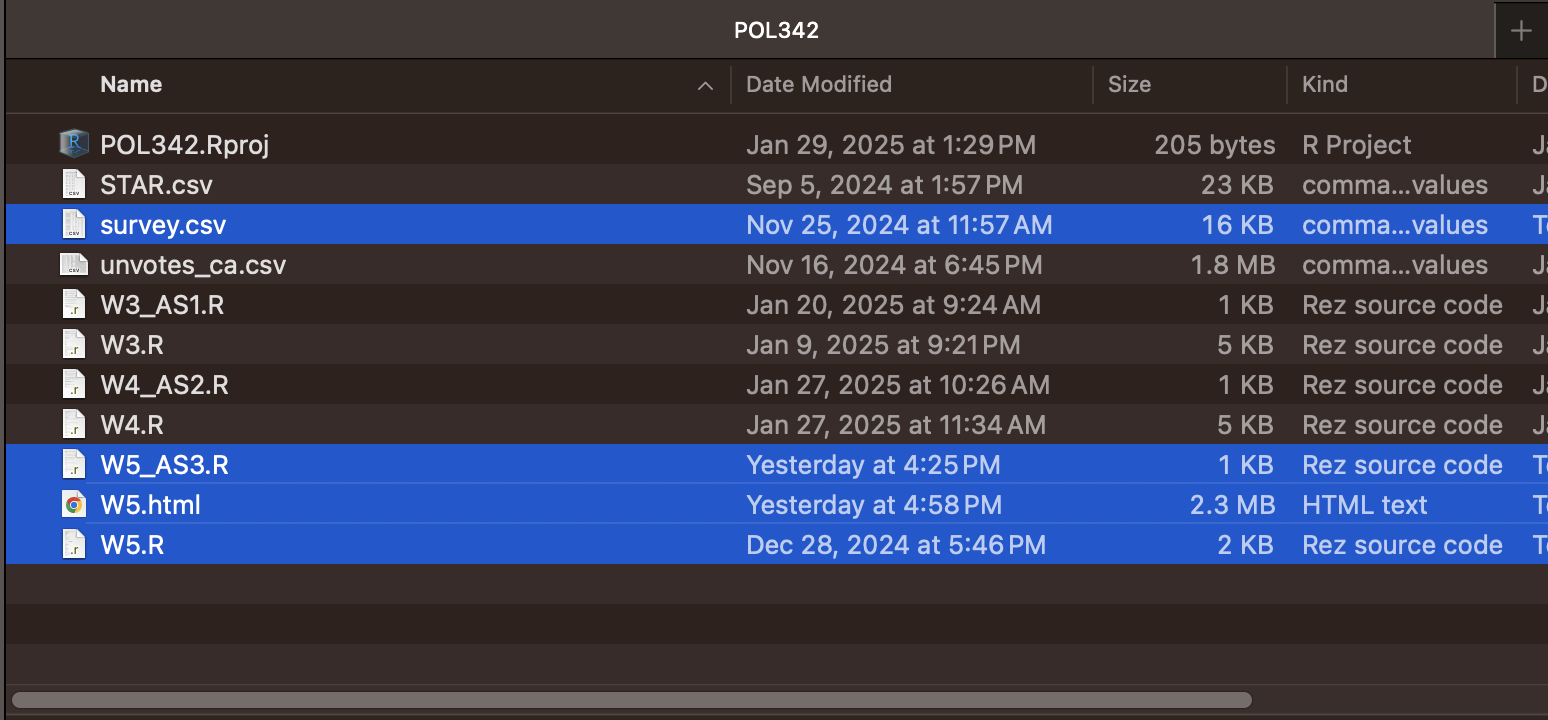
\includegraphics[width=0.7\linewidth]{images/w5} \end{center}

\subsection*{Install new package and load all packages required for this class}\label{install-new-package-and-load-all-packages-required-for-this-class}
\addcontentsline{toc}{subsection}{Install new package and load all packages required for this class}

\begin{Shaded}
\begin{Highlighting}[]
\FunctionTok{install.packages}\NormalTok{(}\StringTok{"sjPlot"}\NormalTok{)}
\FunctionTok{library}\NormalTok{(sjPlot)}

\FunctionTok{library}\NormalTok{(tidyverse)}
\end{Highlighting}
\end{Shaded}

\section{Load data}\label{load-data}

We will be using two data sets today, one from last week---Canada's votes at the UNGA---and the other is an experimental data.

\begin{Shaded}
\begin{Highlighting}[]
\NormalTok{df }\OtherTok{\textless{}{-}} \FunctionTok{read.csv}\NormalTok{(}\StringTok{"unvotes\_ca.csv"}\NormalTok{)}
\NormalTok{survey }\OtherTok{\textless{}{-}} \FunctionTok{read.csv}\NormalTok{(}\StringTok{"survey.csv"}\NormalTok{)}
\end{Highlighting}
\end{Shaded}

\section{Recap and some additional basics}\label{recap-and-some-additional-basics}

\subsection*{R scripts}\label{r-scripts}
\addcontentsline{toc}{subsection}{R scripts}

R scripts should be complete in itself. Before submitting your assignments, start a new session, clear your workspace, select the entire code (i.e.~``Select All'') and run everything. You should not get any errors.

\subsection*{\texorpdfstring{Syntax for functions: \texttt{\textless{}functionname\textgreater{}(\textless{}argument(s)\textgreater{})}}{Syntax for functions: \textless functionname\textgreater(\textless argument(s)\textgreater)}}\label{syntax-for-functions-functionnamearguments}
\addcontentsline{toc}{subsection}{Syntax for functions: \texttt{\textless{}functionname\textgreater{}(\textless{}argument(s)\textgreater{})}}

Functions are a fixed series of actions done to an object. The syntax will always begin with the function name, followed by \texttt{()}.

\begin{center}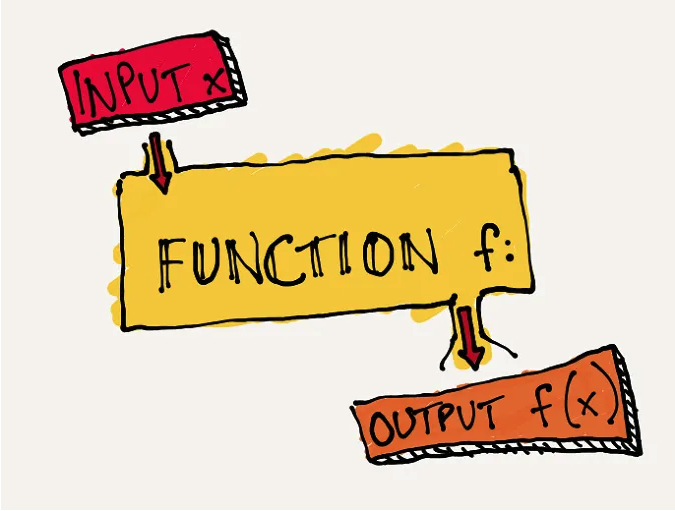
\includegraphics[width=0.7\linewidth]{images/w5_function} \end{center}

(Image credit: \url{https://medium.com/swlh/7-programming-concepts-functions-6072d7c50278})

In some cases, functions may not have arguments, for example, \texttt{n()}. The following is the documentation for \texttt{n()},

\begin{center}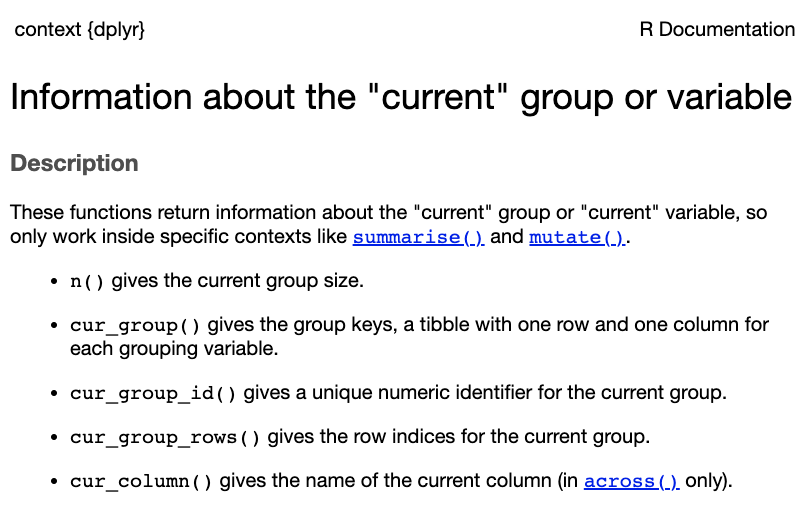
\includegraphics[width=0.7\linewidth]{images/w5_ndocument} \end{center}

\subsection*{Arguments are function-specific}\label{arguments-are-function-specific}
\addcontentsline{toc}{subsection}{Arguments are function-specific}

Last week we learnt the following tidyverse functions

\begin{itemize}
\tightlist
\item
  filter()
\item
  group\_by()
\item
  mutate()
\item
  reframe()
\item
  select()
\item
  arrange()
\end{itemize}

\texttt{filter()} takes expressions that produce a logical value, i.e.~conditional statements

\begin{Shaded}
\begin{Highlighting}[]
\NormalTok{df }\SpecialCharTok{|\textgreater{}}
  \FunctionTok{filter}\NormalTok{(year}\SpecialCharTok{==}\DecValTok{1983} \SpecialCharTok{\&}\NormalTok{ importantvote}\SpecialCharTok{==}\DecValTok{1}\NormalTok{)}
\end{Highlighting}
\end{Shaded}

\begin{verbatim}
##   rcid country country_code year vote session importantvote       date
## 1 2497  Canada           CA 1983  yes      38             1 1983-11-06
## 2 2510  Canada           CA 1983   no      38             1 1983-12-06
## 3 2526  Canada           CA 1983   no      38             1 1983-12-06
## 4 2526  Canada           CA 1983   no      38             1 1983-12-06
## 5 2563  Canada           CA 1983  yes      38             1 1983-12-07
## 6 2610  Canada           CA 1983  yes      38             1 1983-12-03
## 7 2610  Canada           CA 1983  yes      38             1 1983-12-03
##       unres amend para                                short
## 1   R/38/29     0    0                          AFGHANISTAN
## 2  R/38/39G     0    0 SOUTH AFRICA, MILITARY COLLABORATION
## 3 R/38/180E     0    0                    ISRAEL, ISOLATION
## 4 R/38/180E     0    0                    ISRAEL, ISOLATION
## 5 R/38/187C     0    0         CHEMICAL, BIOLOGICAL WEAPONS
## 6  R/38/101     0    0            HUMAN RIGHTS, EL SALVADOR
## 7  R/38/101     0    0            HUMAN RIGHTS, EL SALVADOR
##                                                                                                                                                                                                                                                  descr
## 1                                TO DEMAND THE WITHDRAWAL OF FOREIGN FORCES FROM AFGHANISTAN, TO DECLARE ONCE AGAIN THE RIGHTS OF THE PEOPLE OF AFGHANISTAN TO POLITICAL INDEPENDENCE, AND TO EXTEND A PLEA FOR RELIEF ASSISTANCE FOR AFGHAN REFUGEES.
## 2                            TO RECOMMEND THAT THE SECURITY COUNCIL TAKE STEPS TO MAKE CERTAIN THAT ALL STATES TERMINATE MILITARY AND NUCLEAR COOPERATION WITH THE REGIME OF SOUTH AFRICA AND TO DENOUNCE THOSE STATES THAT CONTINUE SUCH COOPERATION.
## 3                                                                                                                                                                               TO ORDER ALL STATES TO TERMINATE MILITARY AND ECONOMIC SUPPORT ISRAEL.
## 4                                                                                                                                                                               TO ORDER ALL STATES TO TERMINATE MILITARY AND ECONOMIC SUPPORT ISRAEL.
## 5                                                                                                            TO NOTE THE REPORT OF THE SECRETARY-GENERAL ON THE IMPLEMENTATION OF RESOLUTION 37/98D DEALING WITH CHEMICAL AND BACTERIOLOGICAL WEAPONS.
## 6 TO EXPRESS CONCERN THAT INFRINGEMENTS OF HUMAN RIGHTS ARE CONTINUING IN EL SALVADOR, TO SUGGEST THAT NECESSARY ECONOMIC AND SOCIAL REFORMS BE IMPLEMENTED TO RESOLVE THE BASIC INTERNAL CONFLICT THERE, TO URGE THE GOVERNMENT TO PROCEED TOWARD A C
## 7 TO EXPRESS CONCERN THAT INFRINGEMENTS OF HUMAN RIGHTS ARE CONTINUING IN EL SALVADOR, TO SUGGEST THAT NECESSARY ECONOMIC AND SOCIAL REFORMS BE IMPLEMENTED TO RESOLVE THE BASIC INTERNAL CONFLICT THERE, TO URGE THE GOVERNMENT TO PROCEED TOWARD A C
##   short_name                                issue
## 1         hr                         Human rights
## 2         nu Nuclear weapons and nuclear material
## 3         me                 Palestinian conflict
## 4         ec                 Economic development
## 5         di         Arms control and disarmament
## 6         hr                         Human rights
## 7         ec                 Economic development
\end{verbatim}

\texttt{group\_by()} take either variables or conditional statements

\begin{Shaded}
\begin{Highlighting}[]
\NormalTok{df }\SpecialCharTok{|\textgreater{}}
  \FunctionTok{group\_by}\NormalTok{(session)}

\CommentTok{\#or}

\NormalTok{df }\SpecialCharTok{|\textgreater{}}
  \FunctionTok{group\_by}\NormalTok{(year}\SpecialCharTok{\textgreater{}}\DecValTok{1989}\NormalTok{)}
\end{Highlighting}
\end{Shaded}

\texttt{mutate()} and \texttt{reframe()} take variable assignment arguments. For \texttt{mutate()}, the original data frame is retained and new variables/columns are added to the data frame. For \texttt{reframe()} the data frame is reduced to the size of the new object.

\subsection*{Missing values}\label{missing-values}
\addcontentsline{toc}{subsection}{Missing values}

If a variable contains missing (\texttt{NA}) values, summary statistics such as mean() and sum() will return \texttt{NA} unless the argument na.rm is specified TRUE, meaning missing values should be removed.

\begin{Shaded}
\begin{Highlighting}[]
\NormalTok{df }\SpecialCharTok{|\textgreater{}}
  \FunctionTok{reframe}\NormalTok{(}\AttributeTok{imptvote =} \FunctionTok{sum}\NormalTok{(importantvote, }\AttributeTok{na.rm=}\NormalTok{T)) }\CommentTok{\# by default na.rm=FALSE}
\end{Highlighting}
\end{Shaded}

\begin{verbatim}
##   imptvote
## 1      448
\end{verbatim}

\begin{Shaded}
\begin{Highlighting}[]
\NormalTok{df }\SpecialCharTok{|\textgreater{}}
  \FunctionTok{reframe}\NormalTok{(}\AttributeTok{imptvote =} \FunctionTok{sum}\NormalTok{(importantvote))}
\end{Highlighting}
\end{Shaded}

\begin{verbatim}
##   imptvote
## 1       NA
\end{verbatim}

To see if a variable contains missing values, you can use a combination of \texttt{table} and \texttt{is.na()}. \texttt{is.na()} returns a same-length vector of \texttt{TRUE}/\texttt{FALSE} (\texttt{TRUE} if the value is missing and \texttt{FALSE} if the value is present).

\begin{Shaded}
\begin{Highlighting}[]
\FunctionTok{is.na}\NormalTok{(df}\SpecialCharTok{$}\NormalTok{importantvote)}
\end{Highlighting}
\end{Shaded}

\begin{Shaded}
\begin{Highlighting}[]
\FunctionTok{table}\NormalTok{(}\FunctionTok{is.na}\NormalTok{(df}\SpecialCharTok{$}\NormalTok{importantvote))}
\end{Highlighting}
\end{Shaded}

\begin{verbatim}
## 
## FALSE  TRUE 
##  5307   425
\end{verbatim}

This tells us that the variable has 425 missing values.

\texttt{select()} and \texttt{arrange()} take variable names.

\begin{Shaded}
\begin{Highlighting}[]
\NormalTok{df }\SpecialCharTok{|\textgreater{}}
  \FunctionTok{select}\NormalTok{(country, year, issue)}
\end{Highlighting}
\end{Shaded}

\subsection*{Argument names}\label{argument-names}
\addcontentsline{toc}{subsection}{Argument names}

In many of the examples here, I omit the name of the argument. This is fine when we know the order of the arguments or when the function requires only one argument. For example, the following codes are equivalent.

\begin{Shaded}
\begin{Highlighting}[]
\FunctionTok{read.csv}\NormalTok{(}\AttributeTok{file=}\StringTok{"unvotes\_ca.csv"}\NormalTok{, }\AttributeTok{header=}\NormalTok{T)}

\FunctionTok{read.csv}\NormalTok{(}\StringTok{"unvotes\_ca.csv"}\NormalTok{, }\ConstantTok{TRUE}\NormalTok{)}
\end{Highlighting}
\end{Shaded}

But that's only because I stated them in the right sequence. See the documentation,

\begin{Shaded}
\begin{Highlighting}[]
\NormalTok{?read.csv}
\end{Highlighting}
\end{Shaded}

\begin{center}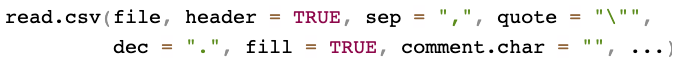
\includegraphics[width=0.7\linewidth]{images/w5_readcsv} \end{center}

Specifying the argument is a safe way to work with unfamiliar functions because it is fine if you get the sequence wrong.

\begin{Shaded}
\begin{Highlighting}[]
\FunctionTok{read.csv}\NormalTok{(}\AttributeTok{header=}\ConstantTok{TRUE}\NormalTok{, }\AttributeTok{file=}\StringTok{"unvotes\_ca.csv"}\NormalTok{)}
\end{Highlighting}
\end{Shaded}

This will give you an error.

\begin{Shaded}
\begin{Highlighting}[]
\FunctionTok{read.csv}\NormalTok{(}\ConstantTok{TRUE}\NormalTok{, }\StringTok{"unvotes\_ca.csv"}\NormalTok{)}
\end{Highlighting}
\end{Shaded}

\subsection*{\texorpdfstring{\texttt{if\_else()} function}{if\_else() function}}\label{if_else-function}
\addcontentsline{toc}{subsection}{\texttt{if\_else()} function}

Let's say we want to create a new binary variable that denotes two separate periods, during and before/after the cold war.

\begin{Shaded}
\begin{Highlighting}[]
\CommentTok{\#read the if\_else() documentation}
\NormalTok{?if\_else}
\end{Highlighting}
\end{Shaded}

\texttt{if\_else} takes a conditional statement as its first argument, followed by the replacement value if \texttt{TRUE} as the second argument, and replacement value if \texttt{FALSE} as the third argument. (Do you remember what a conditional statement is? See Section \ref{conditional-statements})

\begin{center}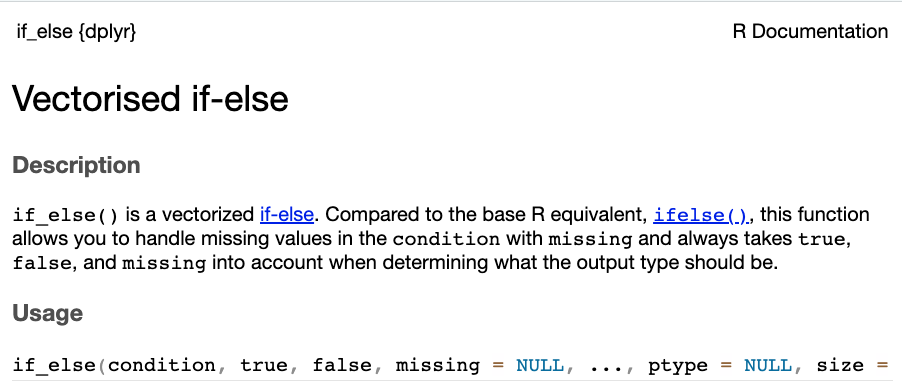
\includegraphics[width=0.7\linewidth]{images/w5_ifelse} \end{center}

\begin{Shaded}
\begin{Highlighting}[]
\NormalTok{df2 }\OtherTok{\textless{}{-}}\NormalTok{ df }\SpecialCharTok{|\textgreater{}} 
  \FunctionTok{mutate}\NormalTok{(}\AttributeTok{support =} \FunctionTok{if\_else}\NormalTok{(vote}\SpecialCharTok{==}\StringTok{"yes"}\NormalTok{, }\CommentTok{\# logical test}
                          \DecValTok{1}\NormalTok{, }\CommentTok{\# TRUE/yes output}
                          \DecValTok{0}\NormalTok{)) }\CommentTok{\# FALSE/no output}
\end{Highlighting}
\end{Shaded}

Find the new variable at the extreme right of the data set.

\begin{Shaded}
\begin{Highlighting}[]
\FunctionTok{View}\NormalTok{(df2)}
\end{Highlighting}
\end{Shaded}

Quick exercise: Explain what each step of the following code executes and what variable \texttt{x} represents in the resultant output.

\begin{Shaded}
\begin{Highlighting}[]
\NormalTok{df }\SpecialCharTok{|\textgreater{}}
  \FunctionTok{group\_by}\NormalTok{(issue, importantvote) }\SpecialCharTok{|\textgreater{}}
  \FunctionTok{reframe}\NormalTok{(}\AttributeTok{n =} \FunctionTok{n}\NormalTok{()) }\SpecialCharTok{|\textgreater{}}
  \FunctionTok{group\_by}\NormalTok{(issue) }\SpecialCharTok{|\textgreater{}}
  \FunctionTok{mutate}\NormalTok{(}\AttributeTok{x =} \FunctionTok{round}\NormalTok{(n}\SpecialCharTok{/}\FunctionTok{sum}\NormalTok{(n), }\DecValTok{2}\NormalTok{))}
\end{Highlighting}
\end{Shaded}

\begin{verbatim}
## # A tibble: 18 x 4
## # Groups:   issue [6]
##    issue                                importantvote     n     x
##    <chr>                                        <int> <int> <dbl>
##  1 Arms control and disarmament                     0   930  0.85
##  2 Arms control and disarmament                     1    48  0.04
##  3 Arms control and disarmament                    NA   110  0.1 
##  4 Colonialism                                      0   902  0.94
##  5 Colonialism                                      1    33  0.03
##  6 Colonialism                                     NA    21  0.02
##  7 Economic development                             0   637  0.84
##  8 Economic development                             1    67  0.09
##  9 Economic development                            NA    58  0.08
## 10 Human rights                                     0   785  0.77
## 11 Human rights                                     1   170  0.17
## 12 Human rights                                    NA    58  0.06
## 13 Nuclear weapons and nuclear material             0   681  0.8 
## 14 Nuclear weapons and nuclear material             1    43  0.05
## 15 Nuclear weapons and nuclear material            NA   129  0.15
## 16 Palestinian conflict                             0   924  0.87
## 17 Palestinian conflict                             1    87  0.08
## 18 Palestinian conflict                            NA    49  0.05
\end{verbatim}

\section{Data visualization}\label{data-visualization-1}

\subsection*{\texorpdfstring{\texttt{ggplot()}}{ggplot()}}\label{ggplot}
\addcontentsline{toc}{subsection}{\texttt{ggplot()}}

The \texttt{ggplot2} package contains functions tailored to making presentable and informative graphs. It works through piecing together separate pieces of graphical components joined by a \texttt{+} sign, beginning with the empty plane specified using the function ggplot().

\begin{Shaded}
\begin{Highlighting}[]
\FunctionTok{ggplot}\NormalTok{()}
\end{Highlighting}
\end{Shaded}

\pandocbounded{
\includegraphics[keepaspectratio]{POL342-tutorial-notes_files/figure-latex/unnamed-chunk-120-1.pdf}}
To begin plotting on \texttt{ggplot()}, you need to specify two components, 1. data, 2. x-axis and/or y-axis.

The x- and y- axes are specified under \texttt{aes()} which refers to aesthetic mappings. Aesthetic mappings describe how variables in the data are mapped to visual properties.

Integer/numeric (class) on x-axis

\begin{Shaded}
\begin{Highlighting}[]
\FunctionTok{ggplot}\NormalTok{(}\AttributeTok{data=}\NormalTok{df, }\FunctionTok{aes}\NormalTok{(}\AttributeTok{x=}\NormalTok{importantvote))}
\end{Highlighting}
\end{Shaded}

\pandocbounded{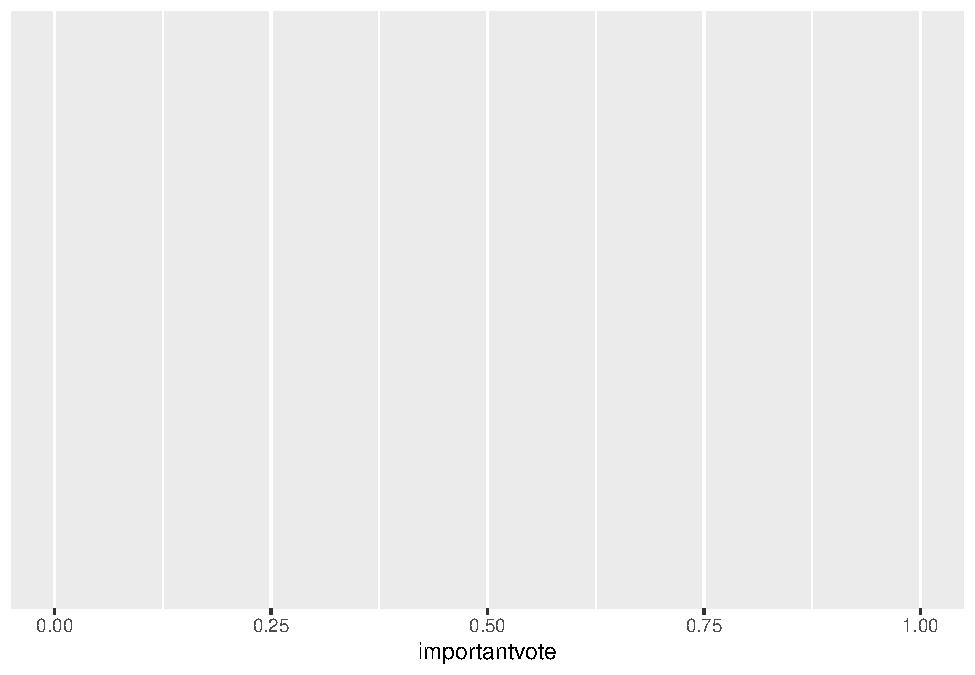
\includegraphics[keepaspectratio]{POL342-tutorial-notes_files/figure-latex/unnamed-chunk-121-1.pdf}}

Character (class) on the y-axis

\begin{Shaded}
\begin{Highlighting}[]
\FunctionTok{ggplot}\NormalTok{(}\AttributeTok{data=}\NormalTok{df, }\FunctionTok{aes}\NormalTok{(}\AttributeTok{y=}\NormalTok{vote))}
\end{Highlighting}
\end{Shaded}

\pandocbounded{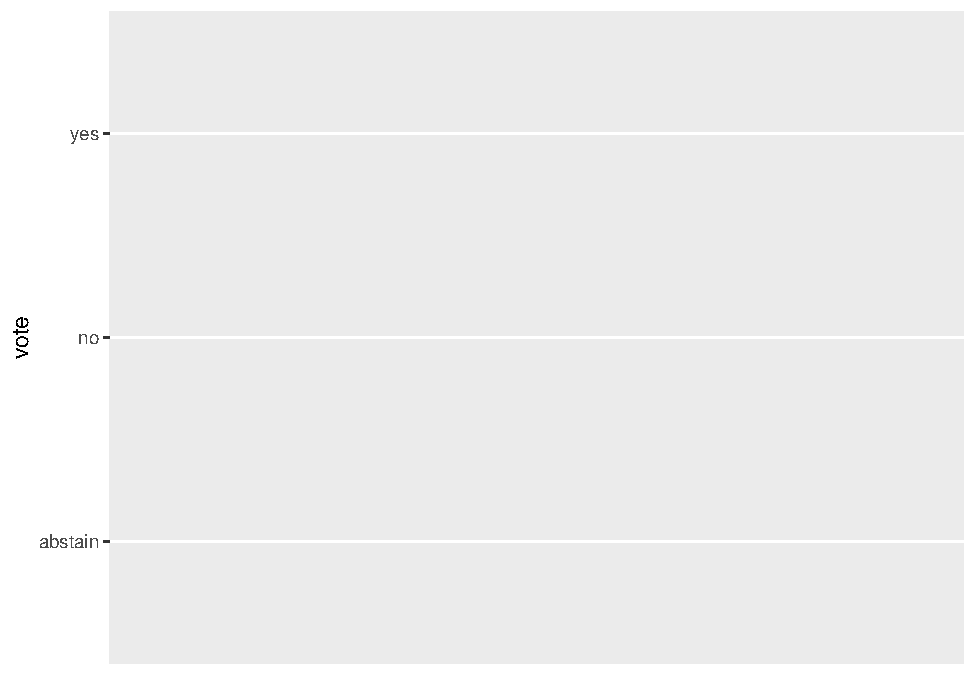
\includegraphics[keepaspectratio]{POL342-tutorial-notes_files/figure-latex/unnamed-chunk-122-1.pdf}}

\section{Plots for categorical variables}\label{plots-for-categorical-variables}

\subsection*{Univariate: nominal/ordinal}\label{univariate-nominalordinal}
\addcontentsline{toc}{subsection}{Univariate: nominal/ordinal}

Create frequency bar charts by adding \texttt{geom\_bar()} to \texttt{ggplot()}

\begin{Shaded}
\begin{Highlighting}[]
\FunctionTok{ggplot}\NormalTok{(df2, }\FunctionTok{aes}\NormalTok{(}\AttributeTok{x=}\NormalTok{vote)) }\SpecialCharTok{+}
  \FunctionTok{geom\_bar}\NormalTok{()}
\end{Highlighting}
\end{Shaded}

\pandocbounded{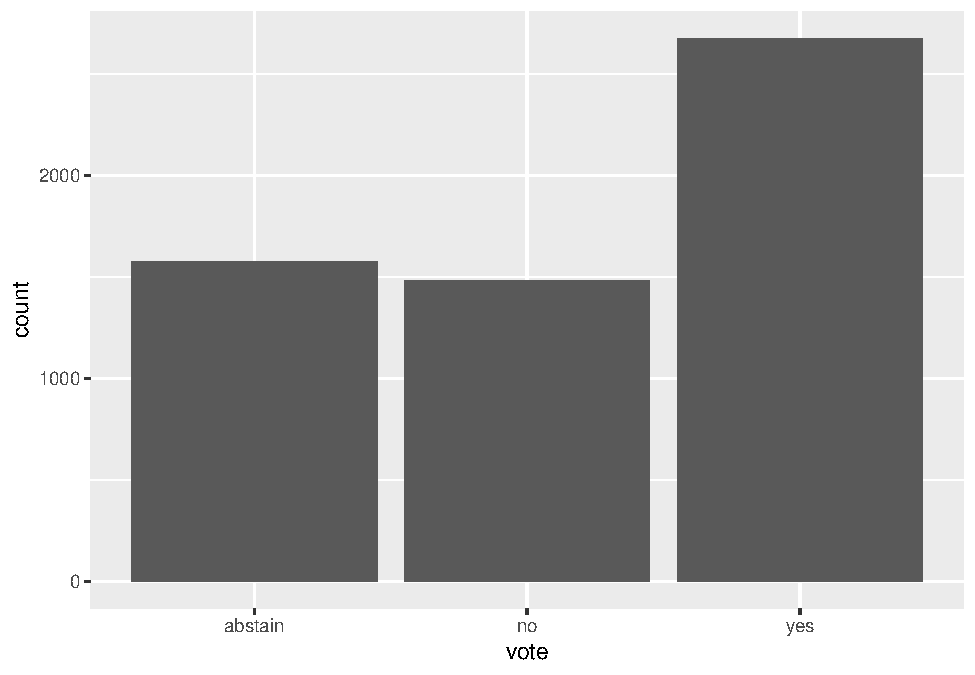
\includegraphics[keepaspectratio]{POL342-tutorial-notes_files/figure-latex/unnamed-chunk-123-1.pdf}}

Note: Do not confuse geom\_bar with another type of bar chart, \texttt{geom\_col()}. \texttt{geom\_bar()} summarizes the data into groups while \texttt{geom\_col()} plots the values in the data.

\begin{Shaded}
\begin{Highlighting}[]
\NormalTok{data }\OtherTok{\textless{}{-}} \FunctionTok{data.frame}\NormalTok{(}\AttributeTok{vote =} \FunctionTok{c}\NormalTok{(}\StringTok{"abstain"}\NormalTok{,}\StringTok{"no"}\NormalTok{,}\StringTok{"yes"}\NormalTok{),}
                   \AttributeTok{count =} \FunctionTok{c}\NormalTok{(}\DecValTok{5}\NormalTok{,}\DecValTok{15}\NormalTok{,}\DecValTok{20}\NormalTok{))}

\FunctionTok{ggplot}\NormalTok{(data, }\FunctionTok{aes}\NormalTok{(}\AttributeTok{x=}\NormalTok{vote,}\AttributeTok{y=}\NormalTok{count)) }\SpecialCharTok{+}
  \FunctionTok{geom\_col}\NormalTok{()}
\end{Highlighting}
\end{Shaded}

\pandocbounded{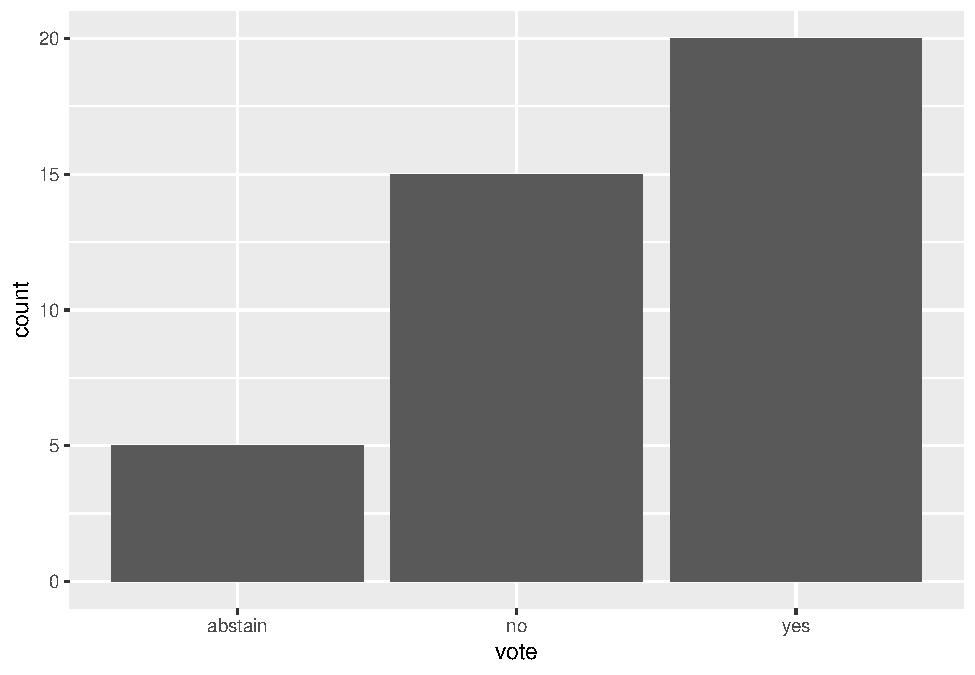
\includegraphics[keepaspectratio]{POL342-tutorial-notes_files/figure-latex/unnamed-chunk-124-1.pdf}}

For clearer presentation of single variables, categories with long names can be plotted on the y-axis instead of x-axis.

\begin{Shaded}
\begin{Highlighting}[]
\CommentTok{\# poor presentation}
\NormalTok{df2 }\SpecialCharTok{|\textgreater{}}
  \FunctionTok{ggplot}\NormalTok{(}\FunctionTok{aes}\NormalTok{(}\AttributeTok{x=}\NormalTok{issue)) }\SpecialCharTok{+}
  \FunctionTok{geom\_bar}\NormalTok{()}
\end{Highlighting}
\end{Shaded}

\pandocbounded{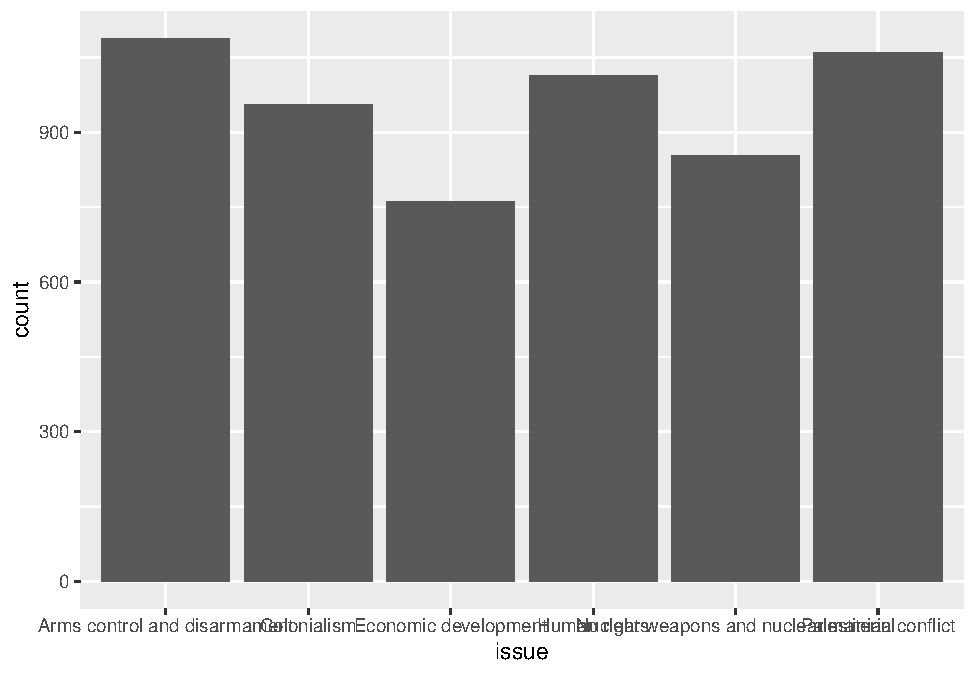
\includegraphics[keepaspectratio]{POL342-tutorial-notes_files/figure-latex/unnamed-chunk-125-1.pdf}}

\begin{Shaded}
\begin{Highlighting}[]
\CommentTok{\# better presentation}
\NormalTok{df2 }\SpecialCharTok{|\textgreater{}}
  \FunctionTok{ggplot}\NormalTok{(}\FunctionTok{aes}\NormalTok{(}\AttributeTok{y=}\NormalTok{issue)) }\SpecialCharTok{+}
  \FunctionTok{geom\_bar}\NormalTok{()}
\end{Highlighting}
\end{Shaded}

\pandocbounded{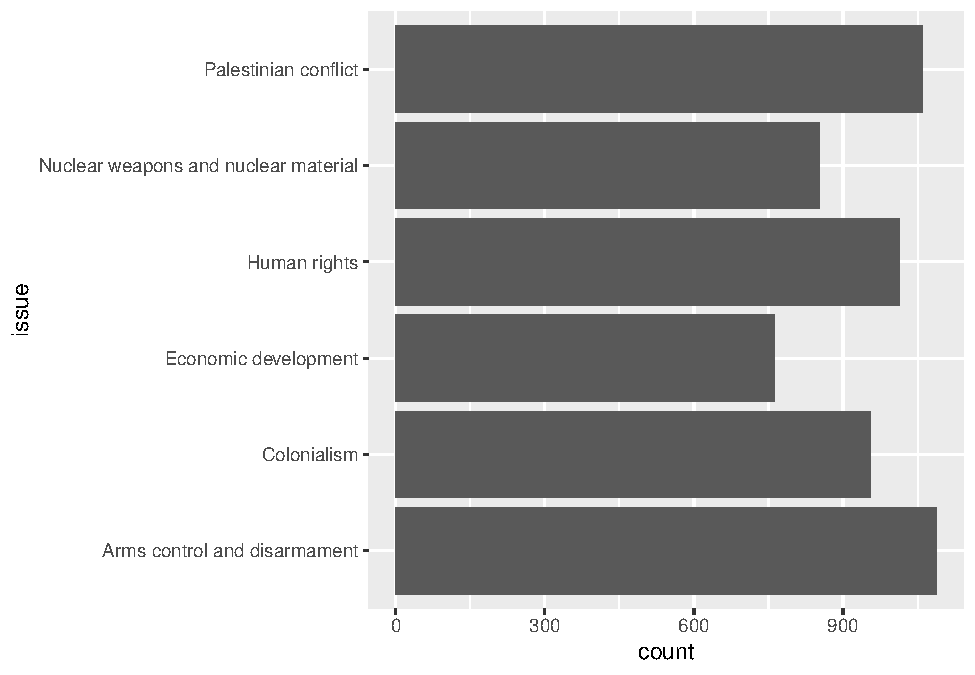
\includegraphics[keepaspectratio]{POL342-tutorial-notes_files/figure-latex/unnamed-chunk-126-1.pdf}}

\subsection*{Bivariate: two nominal/ordinal variables}\label{bivariate-two-nominalordinal-variables}
\addcontentsline{toc}{subsection}{Bivariate: two nominal/ordinal variables}

\begin{itemize}
\tightlist
\item
  Crosstabs and chi-square test -- tab\_xtab()
\end{itemize}

\begin{Shaded}
\begin{Highlighting}[]
\NormalTok{?tab\_xtab}
\end{Highlighting}
\end{Shaded}

\begin{center}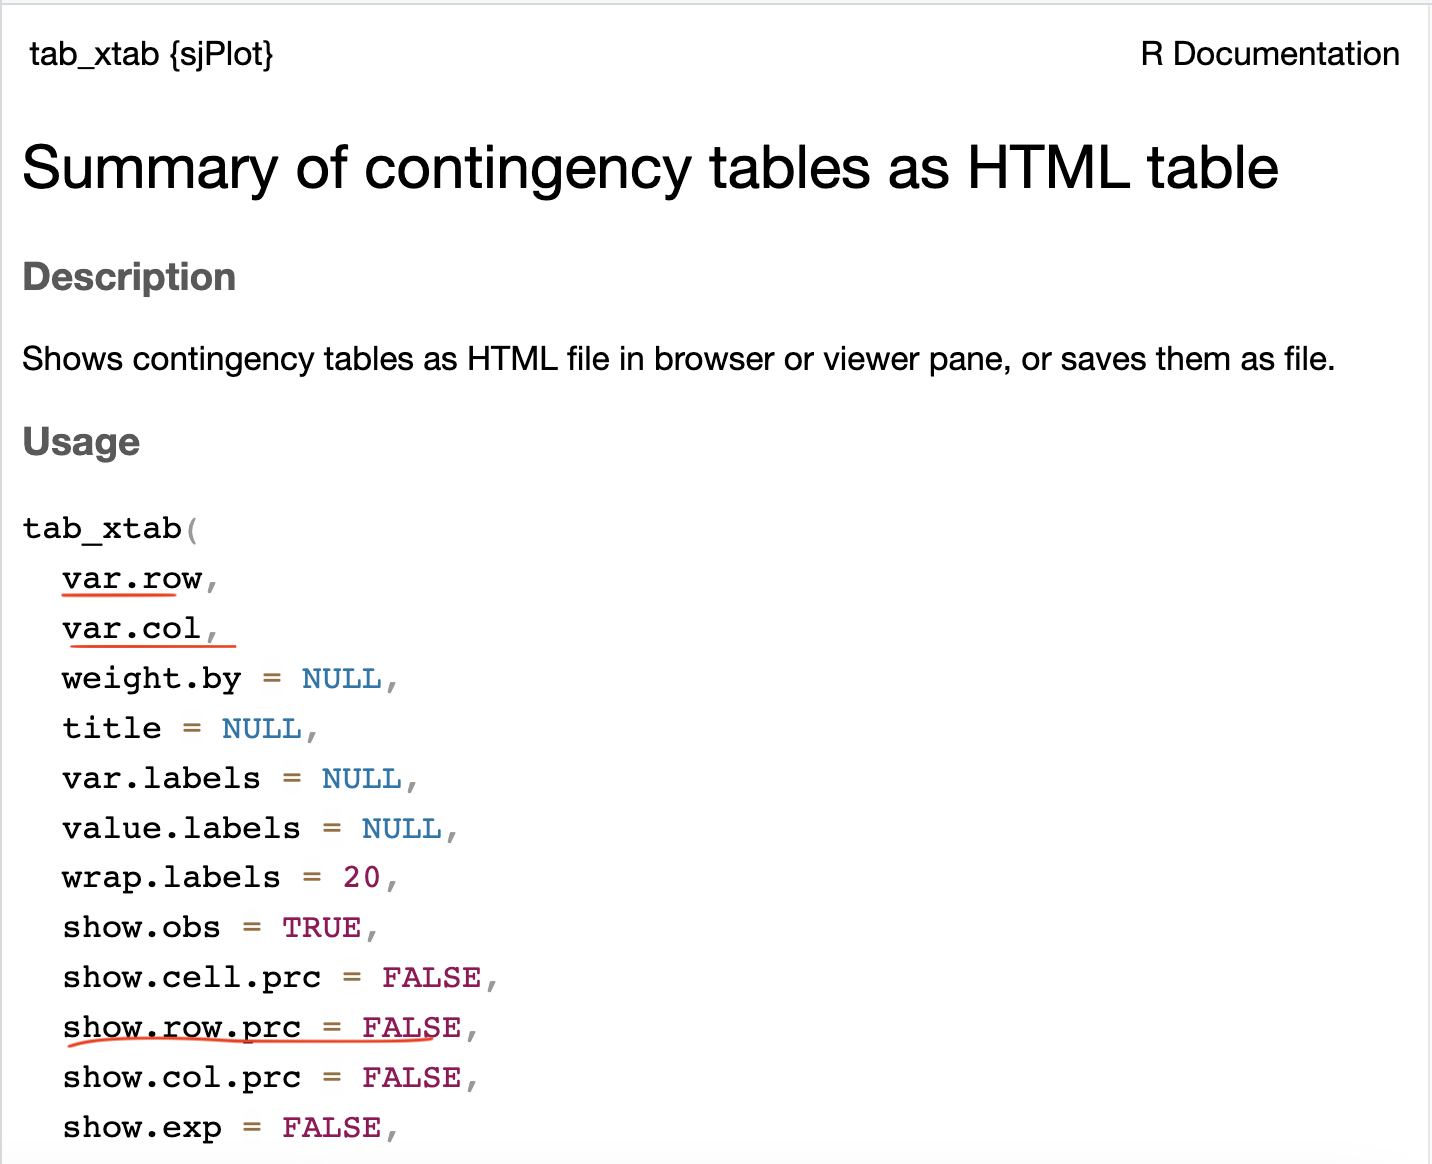
\includegraphics[width=0.7\linewidth]{images/w5_tabxtab} \end{center}

Let's cross-tabulate Canada's votes on the six issues listed in the dataset. Independent variable in columns and dependent variables in rows. (Note: \texttt{tab\_xtab} is not a tidyverse function. Hence, variable names should be preceded by object name of data frame and \texttt{\$})

\begin{Shaded}
\begin{Highlighting}[]
\FunctionTok{tab\_xtab}\NormalTok{(}\AttributeTok{var.col=}\NormalTok{df2}\SpecialCharTok{$}\NormalTok{issue, }\AttributeTok{var.row=}\NormalTok{df2}\SpecialCharTok{$}\NormalTok{vote,}
         \AttributeTok{show.col.prc =} \ConstantTok{TRUE}\NormalTok{,}
         \AttributeTok{show.row.prc =} \ConstantTok{FALSE}\NormalTok{)}
\end{Highlighting}
\end{Shaded}

vote

issue

Total

Arms control anddisarmament

Colonialism

Economic development

Human rights

Nuclear weapons andnuclear material

Palestinian conflict

abstain

{263}{24.2~\%}

{311}{32.5~\%}

{228}{29.9~\%}

{278}{27.4~\%}

{205}{24~\%}

{289}{27.3~\%}

{1574}{27.5~\%}

no

{231}{21.2~\%}

{240}{25.1~\%}

{137}{18~\%}

{338}{33.4~\%}

{236}{27.7~\%}

{301}{28.4~\%}

{1483}{25.9~\%}

yes

{594}{54.6~\%}

{405}{42.4~\%}

{397}{52.1~\%}

{397}{39.2~\%}

{412}{48.3~\%}

{470}{44.3~\%}

{2675}{46.7~\%}

Total

{1088}{100~\%}

{956}{100~\%}

{762}{100~\%}

{1013}{100~\%}

{853}{100~\%}

{1060}{100~\%}

{5732}{100~\%}

χ2=108.983 · df=10 · Cramer's V=0.098 · p=0.000

\begin{itemize}
\tightlist
\item
  Visualizing the contingency table with stacked bar plot
\end{itemize}

What we want:
\pandocbounded{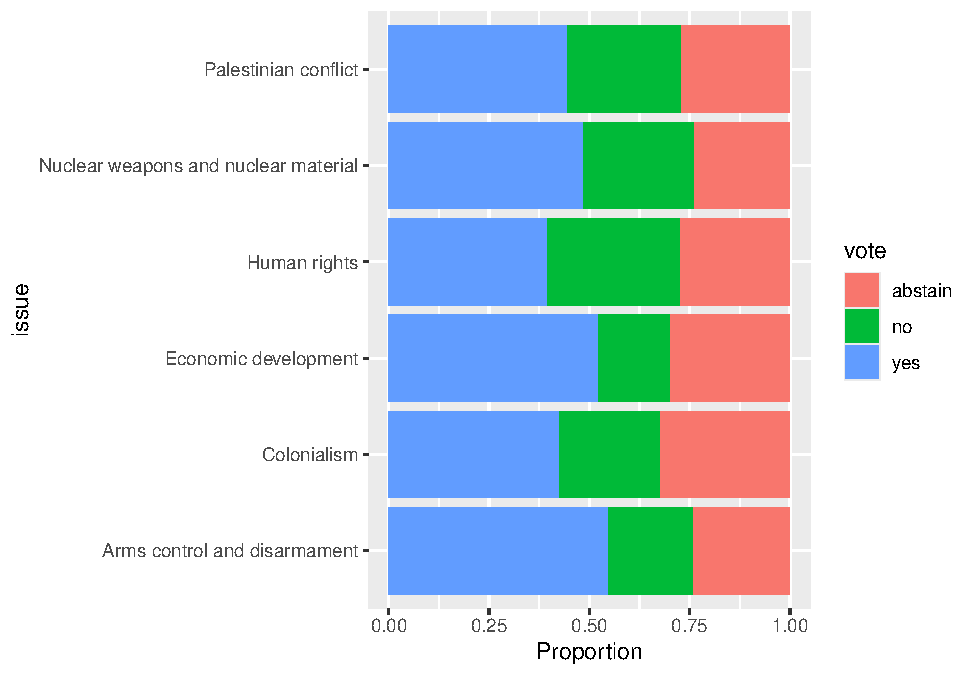
\includegraphics[keepaspectratio]{POL342-tutorial-notes_files/figure-latex/unnamed-chunk-130-1.pdf}}

\textbf{First step: \texttt{geom\_bar()}}

\begin{Shaded}
\begin{Highlighting}[]
\NormalTok{df2 }\SpecialCharTok{|\textgreater{}}
  \FunctionTok{ggplot}\NormalTok{(}\FunctionTok{aes}\NormalTok{(}\AttributeTok{y=}\NormalTok{issue)) }\SpecialCharTok{+}
  \FunctionTok{geom\_bar}\NormalTok{()}
\end{Highlighting}
\end{Shaded}

\pandocbounded{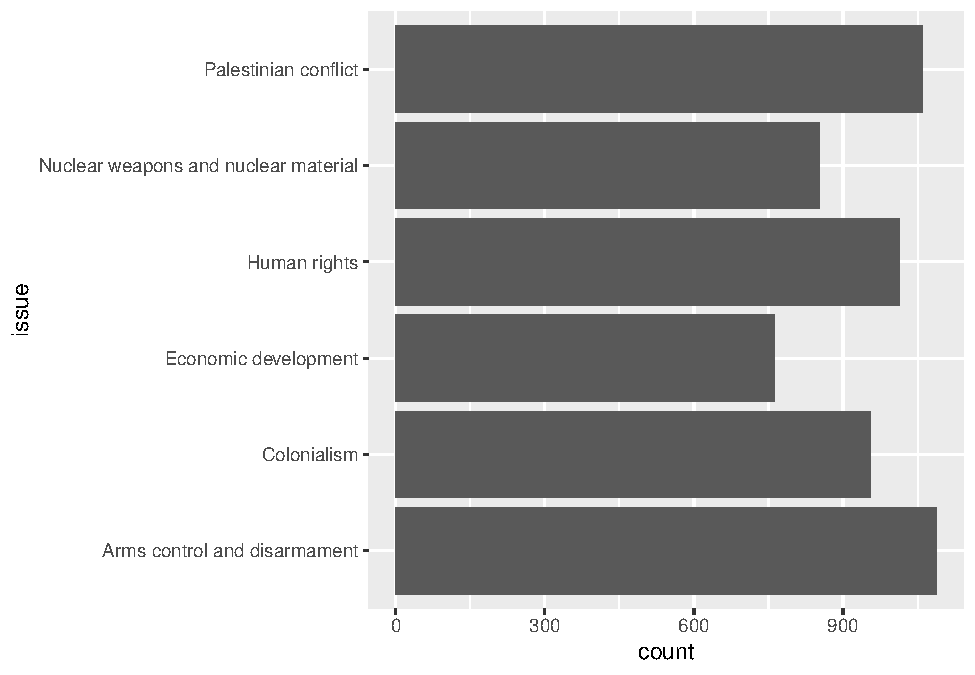
\includegraphics[keepaspectratio]{POL342-tutorial-notes_files/figure-latex/unnamed-chunk-131-1.pdf}}

\textbf{Second step: argument \texttt{fill}}

\begin{Shaded}
\begin{Highlighting}[]
\NormalTok{df2 }\SpecialCharTok{|\textgreater{}}
  \FunctionTok{ggplot}\NormalTok{(}\FunctionTok{aes}\NormalTok{(}\AttributeTok{y=}\NormalTok{issue, }\AttributeTok{fill=}\NormalTok{vote)) }\SpecialCharTok{+}
  \FunctionTok{geom\_bar}\NormalTok{()}
\end{Highlighting}
\end{Shaded}

\pandocbounded{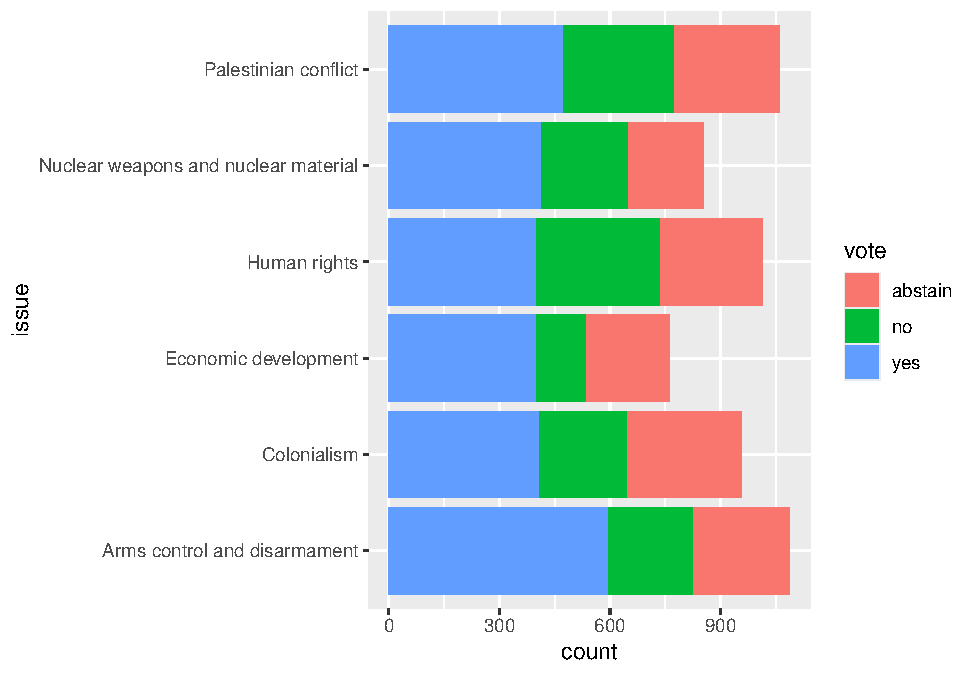
\includegraphics[keepaspectratio]{POL342-tutorial-notes_files/figure-latex/unnamed-chunk-132-1.pdf}}

\textbf{Third step: argument \texttt{position}}

\begin{Shaded}
\begin{Highlighting}[]
\NormalTok{df2 }\SpecialCharTok{|\textgreater{}}
  \FunctionTok{ggplot}\NormalTok{(}\FunctionTok{aes}\NormalTok{(}\AttributeTok{y=}\NormalTok{issue,}\AttributeTok{fill=}\NormalTok{vote)) }\SpecialCharTok{+}
  \FunctionTok{geom\_bar}\NormalTok{(}\AttributeTok{position=}\StringTok{"fill"}\NormalTok{) }\SpecialCharTok{+} \CommentTok{\# position="fill" sets each bar to the same height of 1}
  \FunctionTok{xlab}\NormalTok{(}\StringTok{"Proportion"}\NormalTok{)}
\end{Highlighting}
\end{Shaded}

\pandocbounded{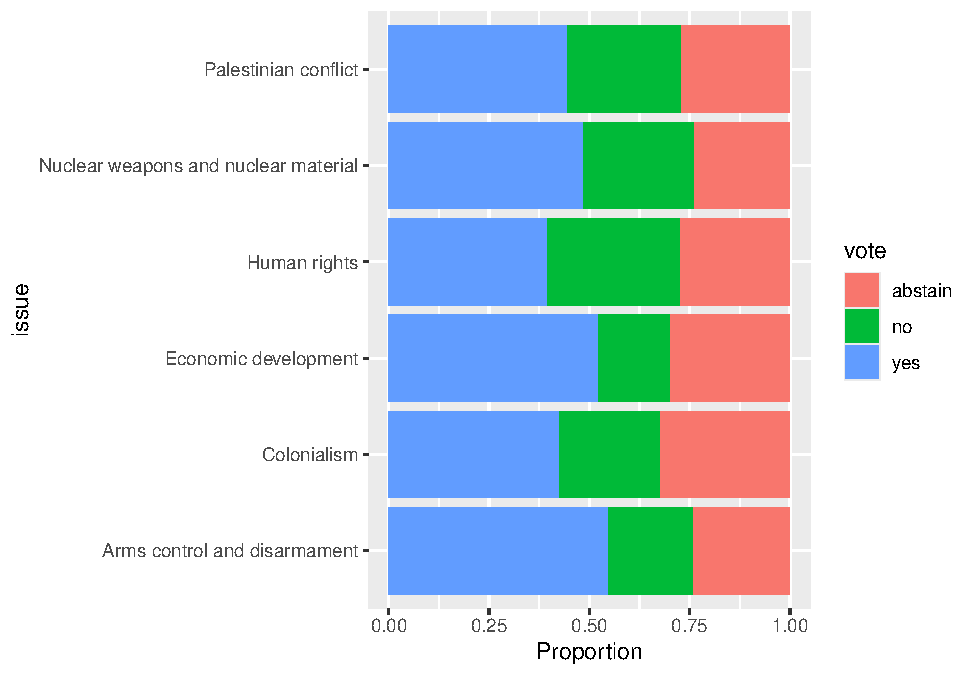
\includegraphics[keepaspectratio]{POL342-tutorial-notes_files/figure-latex/unnamed-chunk-133-1.pdf}}

\section{Plots for interval variables}\label{plots-for-interval-variables}

\subsection*{Survey experiment data}\label{survey-experiment-data}
\addcontentsline{toc}{subsection}{Survey experiment data}

Let us switch data sets here because the UN data set does not contain suitable interval/ratio variables for us to play with.

The data used in the following section is sourced from the replication data of the paper,\\
Lee, Nathan. ``Do Policy Makers Listen to Experts? Evidence from a National Survey of Local and State Policy Makers.'' American Political Science Review 116, no. 2 (2022): 677--88. ~\url{https://doi.org/10.1017/S0003055421000800}.\\
Replication data file: \url{https://dataverse.harvard.edu/dataset.xhtml?persistentId=doi:10.7910/DVN/S2SNOT}

Data comes from a survey fielded to policymakers (elected municipal officials, elected county officials, state legislators, state legislative staffers)

We use a simplified version of the data:

\begin{longtable}[]{@{}
  >{\raggedright\arraybackslash}p{(\linewidth - 2\tabcolsep) * \real{0.1531}}
  >{\raggedright\arraybackslash}p{(\linewidth - 2\tabcolsep) * \real{0.8469}}@{}}
\toprule\noalign{}
\begin{minipage}[b]{\linewidth}\raggedright
variable
\end{minipage} & \begin{minipage}[b]{\linewidth}\raggedright
desc.
\end{minipage} \\
\midrule\noalign{}
\endhead
\bottomrule\noalign{}
\endlastfoot
issue & Needle exchange (1 out of 3 issues discussed in the paper). \\
treated & 1 if treated, 0 if control. Treatment: Experts from several universities have examined this issue and concluded that needle exchanges do not increase drug use. \\
preference & Dependent variable 1: policy preferences (scaled 0-1). Do you support needle exchange? (Strongly support -- Strongly oppose) \\
accuracy & Dependent variable 2: belief accuracy (scaled 0-1). If you were to guess, what percentage of public health experts who conduct research related to needle exchanges believe these programs do NOT increase drug use? (Less than 20\%, 20 - 40\%, 40 - 60\%, 60 - 80\%, More than 80\%) \\
republican & Party affiliation of the policymaker (1 if Republican, 0 if Democrat) \\
age & Age of the policymaker \\
gov\_exp & Over your career, how many years have you worked in government? \\
\end{longtable}

Take a look at the data.

\begin{Shaded}
\begin{Highlighting}[]
\FunctionTok{View}\NormalTok{(survey)}
\end{Highlighting}
\end{Shaded}

\subsection*{Univariate: interval}\label{univariate-interval}
\addcontentsline{toc}{subsection}{Univariate: interval}

Create histograms by adding \texttt{geom\_histogram()} to \texttt{ggplot()}

\begin{Shaded}
\begin{Highlighting}[]
\NormalTok{survey }\SpecialCharTok{|\textgreater{}}
  \FunctionTok{ggplot}\NormalTok{(}\FunctionTok{aes}\NormalTok{(}\AttributeTok{x=}\NormalTok{age)) }\SpecialCharTok{+}
  \FunctionTok{geom\_histogram}\NormalTok{()}
\end{Highlighting}
\end{Shaded}

\pandocbounded{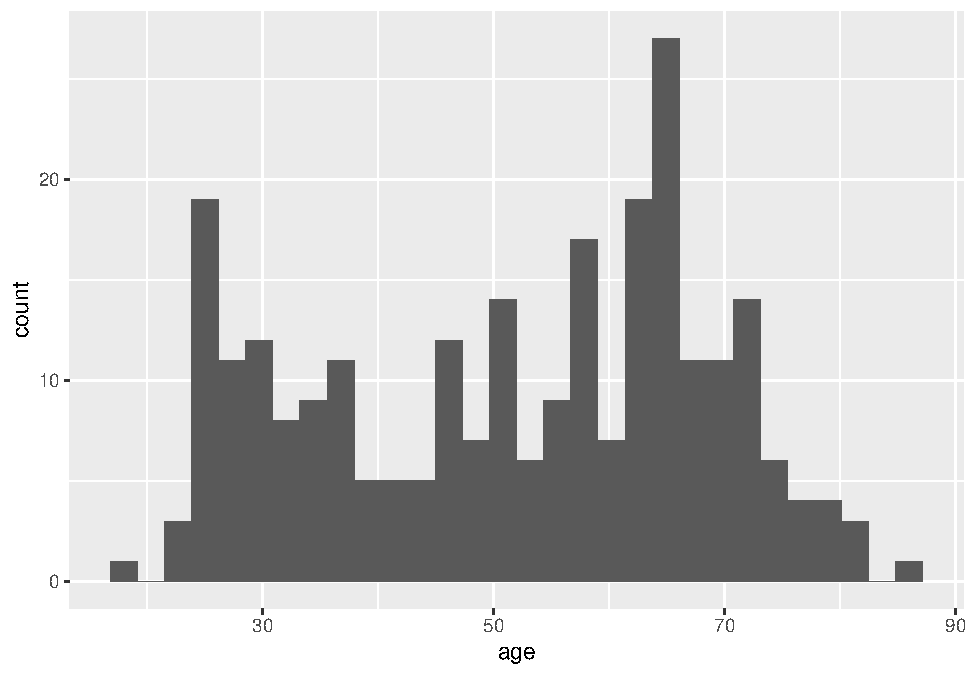
\includegraphics[keepaspectratio]{POL342-tutorial-notes_files/figure-latex/unnamed-chunk-135-1.pdf}}

\subsection*{Bivariate: nominal/ordinal and interval}\label{bivariate-nominalordinal-and-interval}
\addcontentsline{toc}{subsection}{Bivariate: nominal/ordinal and interval}

\textbf{Note: numeric class objects are treated as continuous variables}

\begin{Shaded}
\begin{Highlighting}[]
\FunctionTok{class}\NormalTok{(survey}\SpecialCharTok{$}\NormalTok{treated)}
\end{Highlighting}
\end{Shaded}

\begin{verbatim}
## [1] "integer"
\end{verbatim}

Box and whiskers by group -- \texttt{geom\_boxplot()}

\begin{Shaded}
\begin{Highlighting}[]
\CommentTok{\# incorrect plot}
\NormalTok{survey }\SpecialCharTok{|\textgreater{}}
  \FunctionTok{ggplot}\NormalTok{(}\FunctionTok{aes}\NormalTok{(}\AttributeTok{x=}\NormalTok{republican,}\AttributeTok{y=}\NormalTok{age)) }\SpecialCharTok{+}
  \FunctionTok{geom\_boxplot}\NormalTok{()}
\end{Highlighting}
\end{Shaded}

\pandocbounded{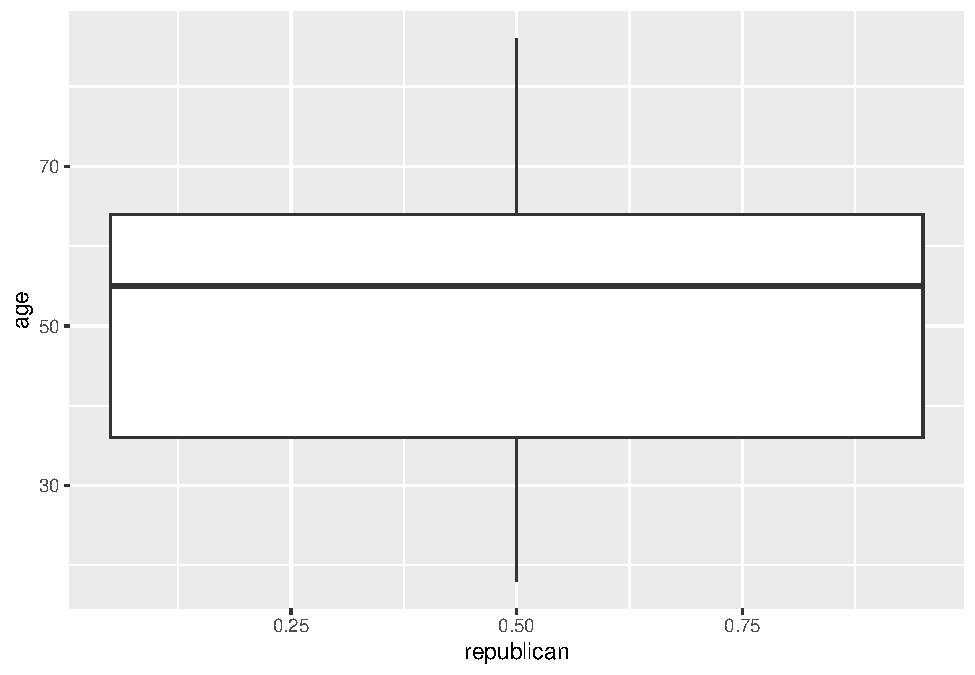
\includegraphics[keepaspectratio]{POL342-tutorial-notes_files/figure-latex/unnamed-chunk-137-1.pdf}}

** Factor class **

\begin{Shaded}
\begin{Highlighting}[]
\FunctionTok{class}\NormalTok{(}\FunctionTok{factor}\NormalTok{(survey}\SpecialCharTok{$}\NormalTok{republican))}
\end{Highlighting}
\end{Shaded}

\begin{verbatim}
## [1] "factor"
\end{verbatim}

Corrected using \texttt{factor()}

\begin{Shaded}
\begin{Highlighting}[]
\NormalTok{survey }\SpecialCharTok{|\textgreater{}}
  \FunctionTok{ggplot}\NormalTok{(}\FunctionTok{aes}\NormalTok{(}\AttributeTok{x=}\FunctionTok{factor}\NormalTok{(republican),}\AttributeTok{y=}\NormalTok{age)) }\SpecialCharTok{+}
  \FunctionTok{geom\_boxplot}\NormalTok{()}
\end{Highlighting}
\end{Shaded}

\pandocbounded{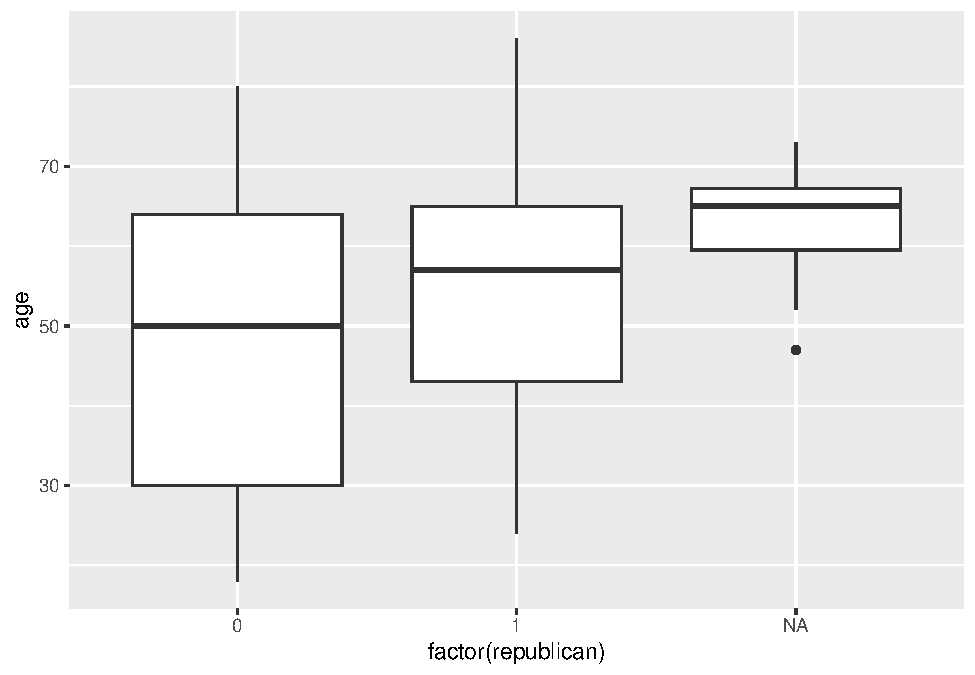
\includegraphics[keepaspectratio]{POL342-tutorial-notes_files/figure-latex/unnamed-chunk-139-1.pdf}}

\subsection*{Bivariate: two interval variables}\label{bivariate-two-interval-variables}
\addcontentsline{toc}{subsection}{Bivariate: two interval variables}

Scatter plot \texttt{geom\_point()}

\begin{Shaded}
\begin{Highlighting}[]
\FunctionTok{ggplot}\NormalTok{(survey,}\FunctionTok{aes}\NormalTok{(}\AttributeTok{x=}\NormalTok{age,}\AttributeTok{y=}\NormalTok{gov\_exp)) }\SpecialCharTok{+}
  \FunctionTok{geom\_point}\NormalTok{()}
\end{Highlighting}
\end{Shaded}

\pandocbounded{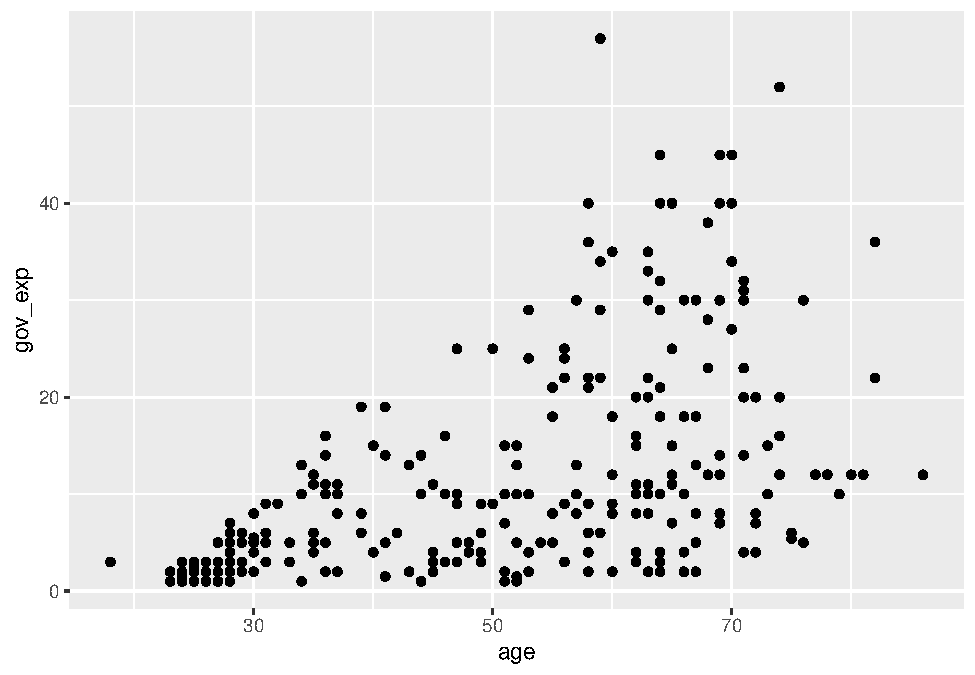
\includegraphics[keepaspectratio]{POL342-tutorial-notes_files/figure-latex/unnamed-chunk-140-1.pdf}}

\section{Credits}\label{credits-2}

\begin{itemize}
\tightlist
\item
  This lesson includes materials from

  \begin{itemize}
  \tightlist
  \item
    \href{https://github.com/dgrtwo/unvotes}{unvotes}
  \item
    \href{https://clauswilke.com/dataviz/visualizing-amounts.html}{Fundamentals of Data Visualization}
  \end{itemize}
\end{itemize}

\chapter{Regression and confidence intervals}\label{regression-and-confidence-intervals}

\begin{itemize}
\tightlist
\item
  Goals for today's class:

  \begin{itemize}
  \tightlist
  \item
    Difference in means -- \texttt{t.test()}
  \item
    Linear regression -- \texttt{lm()}
  \item
    Visualizing models using \texttt{ggplot}

    \begin{itemize}
    \tightlist
    \item
      estimates and confidence intervals -- \texttt{geom\_pointrange()}
    \item
      regression lines

      \begin{itemize}
      \tightlist
      \item
        \texttt{geom\_smooth()}
      \item
        \texttt{geom\_ribbon()}
      \end{itemize}
    \end{itemize}
  \end{itemize}
\end{itemize}

\section{Before the start of class}\label{before-the-start-of-class}

\subsection*{Download files from Quercus}\label{download-files-from-quercus-1}
\addcontentsline{toc}{subsection}{Download files from Quercus}

\begin{center}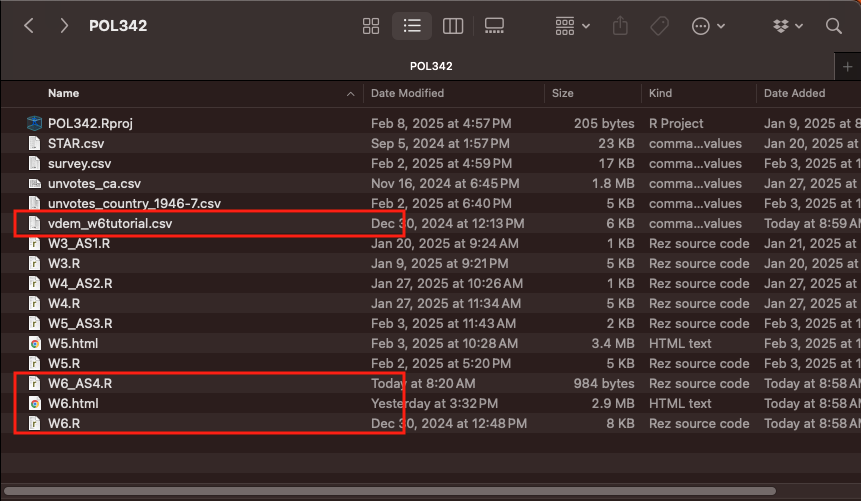
\includegraphics[width=0.7\linewidth]{images/w6} \end{center}

\subsection*{Install new package and load all packages required for this class}\label{install-new-package-and-load-all-packages-required-for-this-class-1}
\addcontentsline{toc}{subsection}{Install new package and load all packages required for this class}

\begin{Shaded}
\begin{Highlighting}[]
\FunctionTok{install.packages}\NormalTok{(}\StringTok{"broom"}\NormalTok{)}
\FunctionTok{library}\NormalTok{(broom)}
\FunctionTok{library}\NormalTok{(tidyverse)}
\end{Highlighting}
\end{Shaded}

\subsection*{Load data}\label{load-data-1}
\addcontentsline{toc}{subsection}{Load data}

\begin{Shaded}
\begin{Highlighting}[]
\NormalTok{df }\OtherTok{\textless{}{-}} \FunctionTok{read.csv}\NormalTok{(}\StringTok{"survey.csv"}\NormalTok{)}
\NormalTok{un\_country }\OtherTok{\textless{}{-}} \FunctionTok{read.csv}\NormalTok{(}\StringTok{"unvotes\_country\_1946{-}7.csv"}\NormalTok{)}
\end{Highlighting}
\end{Shaded}

\section{Recap}\label{recap-1}

\subsection*{Converting variable to factor class}\label{converting-variable-to-factor-class}
\addcontentsline{toc}{subsection}{Converting variable to factor class}

\begin{itemize}
\tightlist
\item
  Republican
\end{itemize}

\begin{Shaded}
\begin{Highlighting}[]
\FunctionTok{class}\NormalTok{(df}\SpecialCharTok{$}\NormalTok{republican)}
\end{Highlighting}
\end{Shaded}

\begin{verbatim}
## [1] "integer"
\end{verbatim}

\begin{itemize}
\tightlist
\item
  ICAO\_region
\end{itemize}

\begin{Shaded}
\begin{Highlighting}[]
\FunctionTok{unique}\NormalTok{(un\_country}\SpecialCharTok{$}\NormalTok{ICAO\_region)}
\end{Highlighting}
\end{Shaded}

\begin{verbatim}
## [1] "ASIAPAC"     "CARSAM"      "EUR"         "NAM"         "MID"        
## [6] "AFI"         "NAT"         "NAM|ASIAPAC"
\end{verbatim}

\begin{Shaded}
\begin{Highlighting}[]
\FunctionTok{ggplot}\NormalTok{(df, }\FunctionTok{aes}\NormalTok{(}\AttributeTok{x=}\FunctionTok{factor}\NormalTok{(republican))) }\SpecialCharTok{+}
  \FunctionTok{geom\_bar}\NormalTok{()}
\end{Highlighting}
\end{Shaded}

\pandocbounded{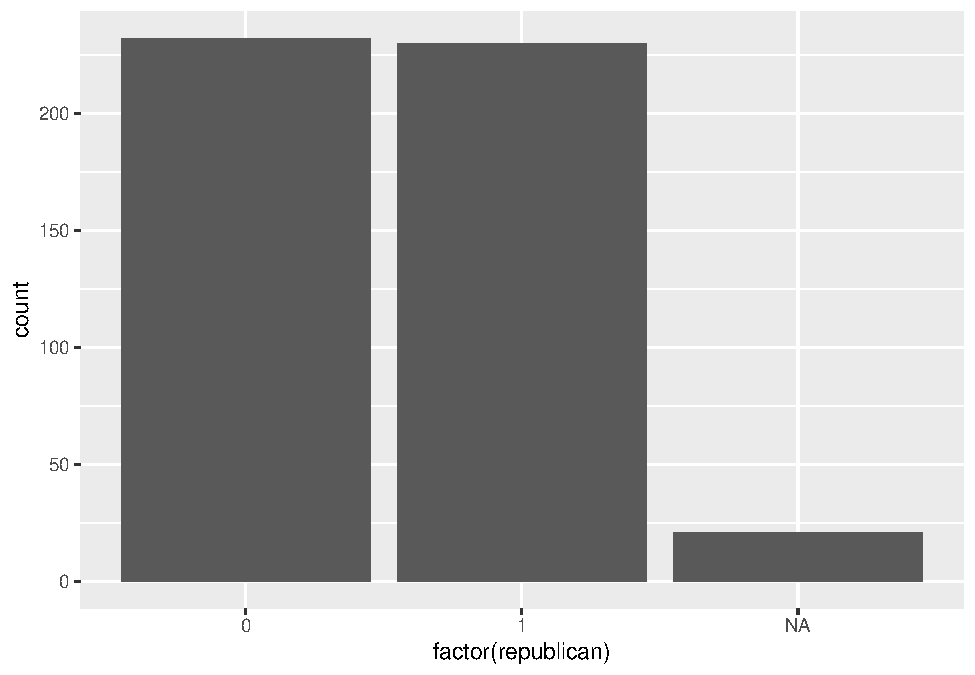
\includegraphics[keepaspectratio]{POL342-tutorial-notes_files/figure-latex/unnamed-chunk-148-1.pdf}}

\subsection*{Determining plot based on type of variable}\label{determining-plot-based-on-type-of-variable}
\addcontentsline{toc}{subsection}{Determining plot based on type of variable}

\begin{itemize}
\tightlist
\item
  Categorical (nominal/ordinal) and categorical -- Stacked bar chart \texttt{geom\_bar}
\item
  Categorical (nominal/ordinal) and numerical (interval/ratio) -- Box and whiskers \texttt{geom\_boxplot}
\item
  Numerical (interval/ratio) and numerical -- Scatter plot \texttt{geom\_point}
\end{itemize}

\begin{Shaded}
\begin{Highlighting}[]
\FunctionTok{ggplot}\NormalTok{(un\_country, }\FunctionTok{aes}\NormalTok{(}\AttributeTok{x=}\NormalTok{ICAO\_region, }\AttributeTok{y=}\NormalTok{share\_yes)) }\SpecialCharTok{+}
  \FunctionTok{geom\_boxplot}\NormalTok{()}
\end{Highlighting}
\end{Shaded}

\pandocbounded{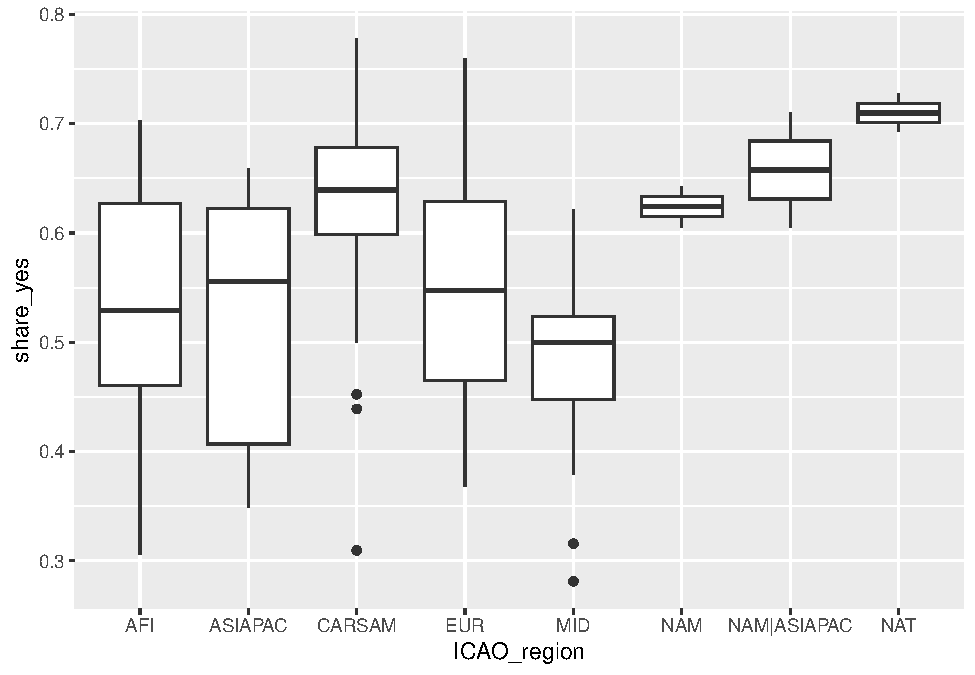
\includegraphics[keepaspectratio]{POL342-tutorial-notes_files/figure-latex/unnamed-chunk-149-1.pdf}}

\section{Experimental study data}\label{experimental-study-data}

Using the same survey data we used last week: the replication data of the paper,\\
Lee, Nathan. ``Do Policy Makers Listen to Experts? Evidence from a National Survey of Local and State Policy Makers.'' American Political Science Review 116, no. 2 (2022): 677--88. ~\url{https://doi.org/10.1017/S0003055421000800}.\\
Replication data file: \url{https://dataverse.harvard.edu/dataset.xhtml?persistentId=doi:10.7910/DVN/S2SNOT}

\subsection*{Outcomes of interest in the study:}\label{outcomes-of-interest-in-the-study}
\addcontentsline{toc}{subsection}{Outcomes of interest in the study:}

\begin{enumerate}
\def\labelenumi{\arabic{enumi}.}
\tightlist
\item
  Beliefs about experts (If you were to guess, what percentage of public health experts who conduct research related to needle exchanges believe these programs do NOT increase drug use? \{Less than 20\%, 20--40\%, 40--60\%, 60--80\%, More than 80\%\})\\
\item
  Policy preferences (Do you support or oppose the use of \{needle exchange programs)? \{Strongly support, Moderately support, Slightly support, Neither support nor oppose, Slightly oppose, Moderately oppose, Strongly oppose.\}
\end{enumerate}

\subsection*{Treatment}\label{treatment}
\addcontentsline{toc}{subsection}{Treatment}

The study implements two types of experiments but we focus only on one aspect of it involving cross-subject design (i.e.~participants are split into treatment and control groups). The theory being tested is \emph{accuracy-motivated reasoning}. The authors hypothesize that policy makers will update their beliefs and preferences following exposure to information about experts. Three policy issues, with high degree of expert consensus but are highly politicized, are utilized in the study. We look at one of the issues on needle exchange.

Here is an excerpt of the treatment:\\
A needle exchange program is a social service which provides clean needles to
drug users to reduce the spread of disease (like HIV or Hepatitis C). However, some people think
these programs encourage drug use.\\
{[}(Treatment) Experts from several universities have examined this issue and concluded that needle exchanges do not increase drug use.{]}

\subsection*{Data}\label{data}
\addcontentsline{toc}{subsection}{Data}

survey fielded to policymakers (elected municipal officials, elected county officials, state legislators, state legislative staffers)

Display first five rows of the dataset.

\begin{Shaded}
\begin{Highlighting}[]
\FunctionTok{head}\NormalTok{(df,}\DecValTok{5}\NormalTok{)}
\end{Highlighting}
\end{Shaded}

\begin{verbatim}
##             issue treated accuracy preference republican age gov_exp
## 1 Needle Exchange       0     0.25      0.000          1  NA      15
## 2 Needle Exchange       1     0.75      0.833          0  NA      25
## 3 Needle Exchange       1     0.50      0.333          1  45      11
## 4 Needle Exchange       1     0.00      0.333          1  NA       5
## 5 Needle Exchange       1     0.25      1.000          1  63       2
\end{verbatim}

\section{\texorpdfstring{Difference in means -- \texttt{t.test()}}{Difference in means -- t.test()}}\label{difference-in-means-t.test}

\subsection*{Syntax}\label{syntax}
\addcontentsline{toc}{subsection}{Syntax}

\begin{center}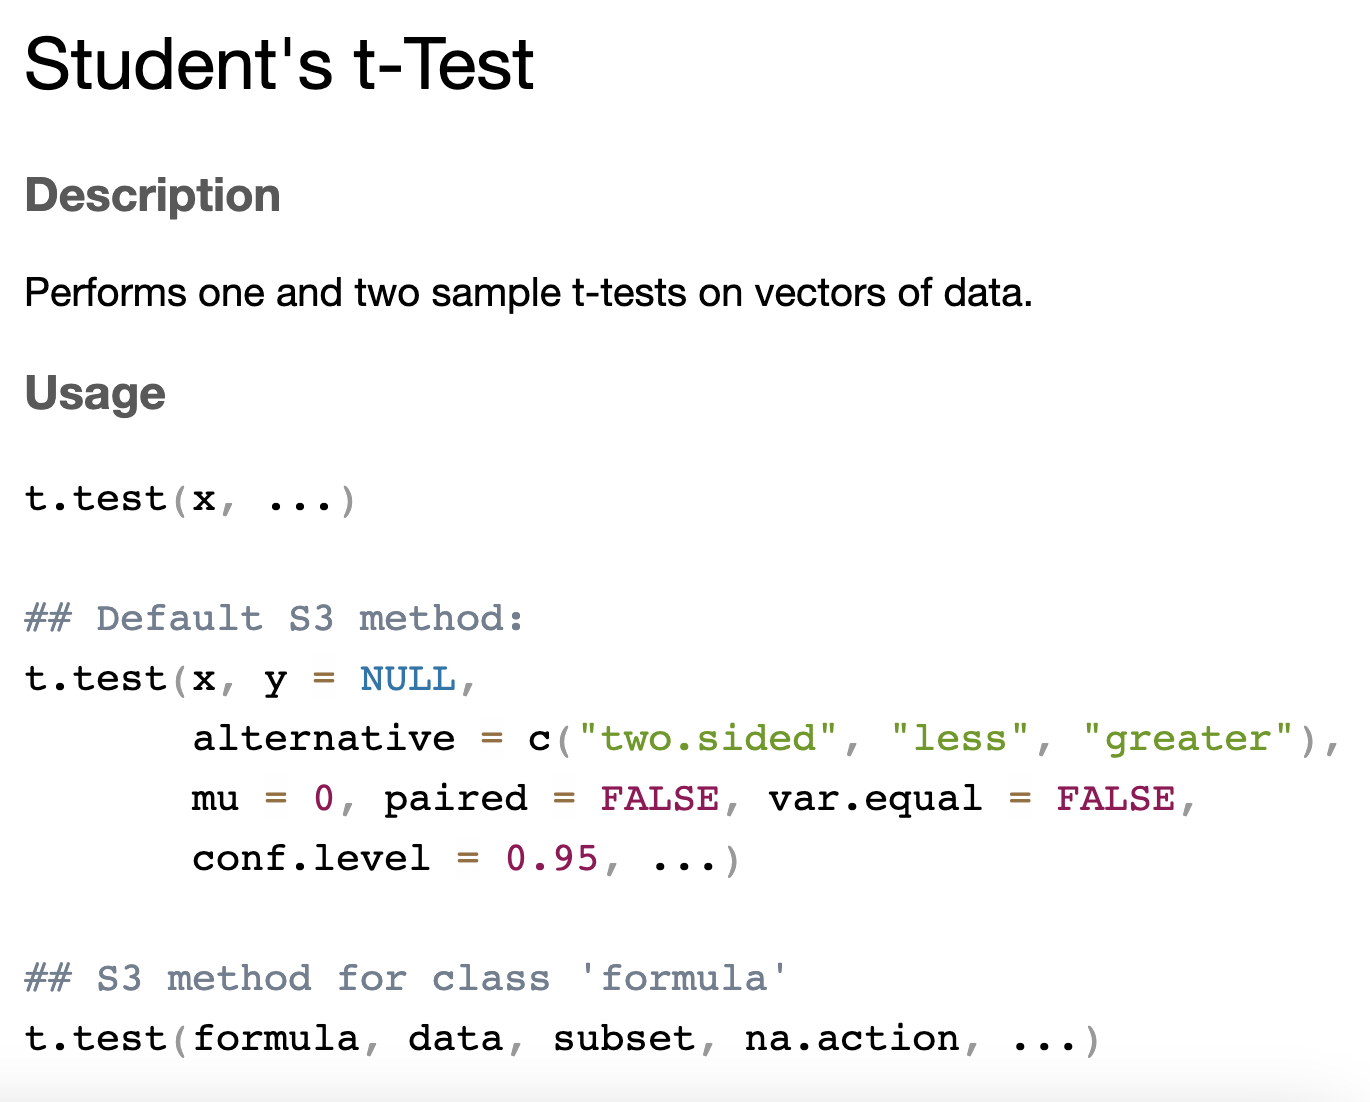
\includegraphics[width=0.7\linewidth]{images/w6_ttest} \end{center}

We are going to use the method involving a formula and data. Formulas are written in R by stating the name of the dependent variable and independent variable, separated by a \texttt{\textasciitilde{}}. In the case of experiments, the independent variable is the treatment and the dependent variable is the outcome of interest, i.e.~\texttt{OutcomeOfInterest\ \textasciitilde{}\ Treatment}.

\subsection*{Outcome 1: Beliefs about experts}\label{outcome-1-beliefs-about-experts}
\addcontentsline{toc}{subsection}{Outcome 1: Beliefs about experts}

Be careful of the direction of the difference. By default, \texttt{t.test()} takes the mean of group 0 - mean of group 1 (in numerical order, alphabetical if the groups are denoted by strings).

\begin{Shaded}
\begin{Highlighting}[]
\FunctionTok{t.test}\NormalTok{(accuracy }\SpecialCharTok{\textasciitilde{}}\NormalTok{ treated, }\AttributeTok{data =}\NormalTok{ df)}
\end{Highlighting}
\end{Shaded}

\begin{verbatim}
## 
##  Welch Two Sample t-test
## 
## data:  accuracy by treated
## t = -3.7138, df = 447.12, p-value = 0.00023
## alternative hypothesis: true difference in means between group 0 and group 1 is not equal to 0
## 95 percent confidence interval:
##  -0.15112544 -0.04652911
## sample estimates:
## mean in group 0 mean in group 1 
##       0.6655405       0.7643678
\end{verbatim}

In order to get the right direction of the effect, we need to reverse the factor order.

\begin{Shaded}
\begin{Highlighting}[]
\FunctionTok{t.test}\NormalTok{(accuracy }\SpecialCharTok{\textasciitilde{}} \FunctionTok{factor}\NormalTok{(treated, }\AttributeTok{levels=}\FunctionTok{c}\NormalTok{(}\DecValTok{1}\NormalTok{,}\DecValTok{0}\NormalTok{)), }\AttributeTok{data =}\NormalTok{ df)}
\end{Highlighting}
\end{Shaded}

\begin{verbatim}
## 
##  Welch Two Sample t-test
## 
## data:  accuracy by factor(treated, levels = c(1, 0))
## t = 3.7138, df = 447.12, p-value = 0.00023
## alternative hypothesis: true difference in means between group 1 and group 0 is not equal to 0
## 95 percent confidence interval:
##  0.04652911 0.15112544
## sample estimates:
## mean in group 1 mean in group 0 
##       0.7643678       0.6655405
\end{verbatim}

\subsection*{Outcome 2: Policy preferences}\label{outcome-2-policy-preferences}
\addcontentsline{toc}{subsection}{Outcome 2: Policy preferences}

\begin{Shaded}
\begin{Highlighting}[]
\FunctionTok{t.test}\NormalTok{(preference }\SpecialCharTok{\textasciitilde{}} \FunctionTok{factor}\NormalTok{(treated, }\AttributeTok{levels=}\FunctionTok{c}\NormalTok{(}\DecValTok{1}\NormalTok{,}\DecValTok{0}\NormalTok{)), }\AttributeTok{data =}\NormalTok{ df)}
\end{Highlighting}
\end{Shaded}

\begin{verbatim}
## 
##  Welch Two Sample t-test
## 
## data:  preference by factor(treated, levels = c(1, 0))
## t = 1.3409, df = 440.32, p-value = 0.1807
## alternative hypothesis: true difference in means between group 1 and group 0 is not equal to 0
## 95 percent confidence interval:
##  -0.01759111  0.09313289
## sample estimates:
## mean in group 1 mean in group 0 
##       0.6909195       0.6531486
\end{verbatim}

\section{Visualizing treatment effects}\label{visualizing-treatment-effects}

\subsection*{\texorpdfstring{Extract the output using \texttt{tidy()} from package \texttt{broom}}{Extract the output using tidy() from package broom}}\label{extract-the-output-using-tidy-from-package-broom}
\addcontentsline{toc}{subsection}{Extract the output using \texttt{tidy()} from package \texttt{broom}}

By default, the output from a t.test is stored in its own unique class of output, which makes it hard for us to extract the data. \texttt{broom} is a package that helps us to convert these types of model output into a data frame. In particular, we use the function \texttt{tidy()} from \texttt{broom}. \texttt{tidy()} works on most analysis models in R. The tidy-ed output is as follows,

\begin{Shaded}
\begin{Highlighting}[]
\FunctionTok{t.test}\NormalTok{(accuracy }\SpecialCharTok{\textasciitilde{}} \FunctionTok{factor}\NormalTok{(treated, }\AttributeTok{levels=}\FunctionTok{c}\NormalTok{(}\DecValTok{1}\NormalTok{,}\DecValTok{0}\NormalTok{)), }\AttributeTok{data =}\NormalTok{ df) }\SpecialCharTok{|\textgreater{}}
  \FunctionTok{tidy}\NormalTok{()}
\end{Highlighting}
\end{Shaded}

\begin{verbatim}
## # A tibble: 1 x 10
##   estimate estimate1 estimate2 statistic  p.value parameter conf.low conf.high
##      <dbl>     <dbl>     <dbl>     <dbl>    <dbl>     <dbl>    <dbl>     <dbl>
## 1   0.0988     0.764     0.666      3.71 0.000230      447.   0.0465     0.151
## # i 2 more variables: method <chr>, alternative <chr>
\end{verbatim}

\subsection*{Interpreting the effect}\label{interpreting-the-effect}
\addcontentsline{toc}{subsection}{Interpreting the effect}

\subsubsection*{Mathematical interpretation}\label{mathematical-interpretation}
\addcontentsline{toc}{subsubsection}{Mathematical interpretation}

Exposure to information regarding expert views of the issue led to a 9.88 percentage point increase in belief accuracy. The observed effect is statistically significant.

\subsubsection*{Substantive interpretation}\label{substantive-interpretation}
\addcontentsline{toc}{subsubsection}{Substantive interpretation}

The increase in belief accuracy on the issue of needle exchange suggests that policy makers are receptive to new evidence about expert views.

\subsection*{Estimates and confidence intervals -- geom\_pointrange()}\label{estimates-and-confidence-intervals-geom_pointrange}
\addcontentsline{toc}{subsection}{Estimates and confidence intervals -- geom\_pointrange()}

Using the tidy-ed data frame, we can plot the estimate. Because the estimate is one-dimensional (you only need either x or y), the other dimension can be used as a name label instead of a variable.

\begin{Shaded}
\begin{Highlighting}[]
\FunctionTok{t.test}\NormalTok{(accuracy }\SpecialCharTok{\textasciitilde{}} \FunctionTok{factor}\NormalTok{(treated, }\AttributeTok{levels=}\FunctionTok{c}\NormalTok{(}\DecValTok{1}\NormalTok{,}\DecValTok{0}\NormalTok{)), }\AttributeTok{data =}\NormalTok{ df) }\SpecialCharTok{|\textgreater{}}
  \FunctionTok{tidy}\NormalTok{() }\SpecialCharTok{|\textgreater{}}
  \FunctionTok{ggplot}\NormalTok{(}\FunctionTok{aes}\NormalTok{(}\AttributeTok{y=}\NormalTok{estimate,}\AttributeTok{x=}\StringTok{"belief about experts"}\NormalTok{)) }\SpecialCharTok{+} 
  \FunctionTok{geom\_pointrange}\NormalTok{(}\FunctionTok{aes}\NormalTok{(}\AttributeTok{ymax=}\NormalTok{conf.high,}\AttributeTok{ymin=}\NormalTok{conf.low,))}
\end{Highlighting}
\end{Shaded}

\pandocbounded{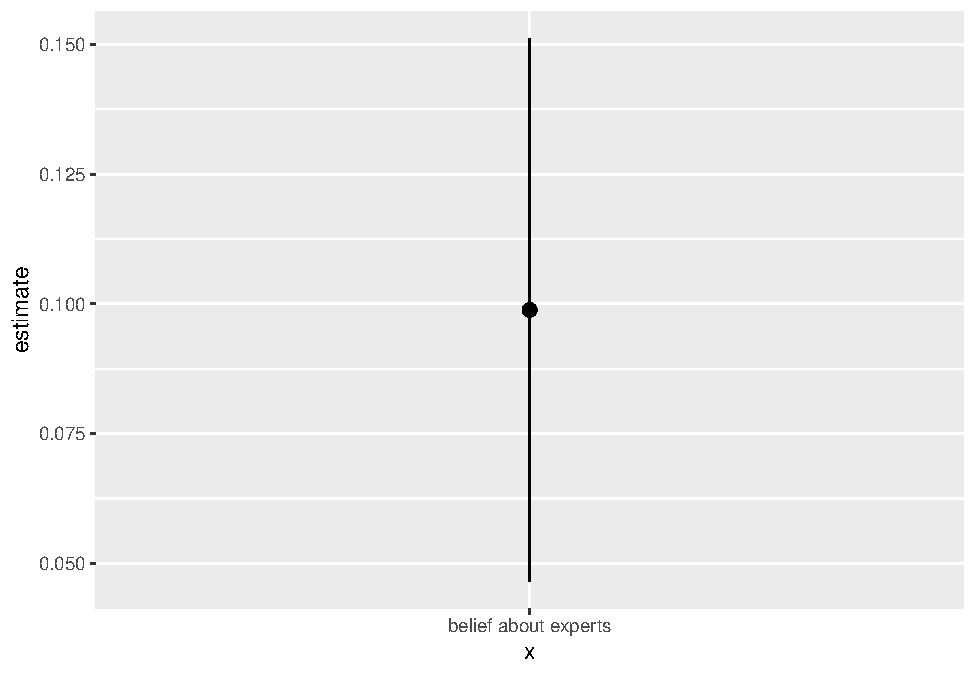
\includegraphics[keepaspectratio]{POL342-tutorial-notes_files/figure-latex/unnamed-chunk-156-1.pdf}}

\texttt{geom\_pointrange()} \textbf{syntax} (\textbf{do not run the following code})

\begin{Shaded}
\begin{Highlighting}[]
\FunctionTok{ggplot}\NormalTok{(}\SpecialCharTok{\textless{}}\NormalTok{name of dataframe}\SpecialCharTok{\textgreater{}}\NormalTok{,}
       \FunctionTok{aes}\NormalTok{(}\AttributeTok{y =}\NormalTok{ estimate, }\CommentTok{\# from the tidy{-}ed output}
           \AttributeTok{x =} \StringTok{"name of x{-}axis label"}\NormalTok{)) }\SpecialCharTok{+} \CommentTok{\# x will be the x{-}axis label}
  \FunctionTok{geom\_pointrange}\NormalTok{(}\FunctionTok{aes}\NormalTok{(}\AttributeTok{ymax=}\NormalTok{conf.high,}\AttributeTok{ymin=}\NormalTok{conf.low)) }\CommentTok{\# from the tidy{-}ed output}
\end{Highlighting}
\end{Shaded}

\subsubsection*{To highlight how the effect is statistically significant, we usually add the 0-intercept line}\label{to-highlight-how-the-effect-is-statistically-significant-we-usually-add-the-0-intercept-line}
\addcontentsline{toc}{subsubsection}{To highlight how the effect is statistically significant, we usually add the 0-intercept line}

\begin{Shaded}
\begin{Highlighting}[]
\FunctionTok{t.test}\NormalTok{(accuracy }\SpecialCharTok{\textasciitilde{}} \FunctionTok{factor}\NormalTok{(treated, }\AttributeTok{levels=}\FunctionTok{c}\NormalTok{(}\DecValTok{1}\NormalTok{,}\DecValTok{0}\NormalTok{)), }\AttributeTok{data =}\NormalTok{ df) }\SpecialCharTok{|\textgreater{}}
  \FunctionTok{tidy}\NormalTok{() }\SpecialCharTok{|\textgreater{}}
  \FunctionTok{ggplot}\NormalTok{(}\FunctionTok{aes}\NormalTok{(}\AttributeTok{y=}\NormalTok{estimate,}\AttributeTok{x=}\StringTok{"belief about experts"}\NormalTok{)) }\SpecialCharTok{+} 
  \FunctionTok{geom\_pointrange}\NormalTok{(}\FunctionTok{aes}\NormalTok{(}\AttributeTok{ymax=}\NormalTok{conf.high,}\AttributeTok{ymin=}\NormalTok{conf.low)) }\SpecialCharTok{+}
  \FunctionTok{geom\_hline}\NormalTok{(}\FunctionTok{aes}\NormalTok{(}\AttributeTok{yintercept=}\DecValTok{0}\NormalTok{),}\AttributeTok{linetype=}\StringTok{"dashed"}\NormalTok{) }\CommentTok{\# this adds a horizontal line}
\end{Highlighting}
\end{Shaded}

\pandocbounded{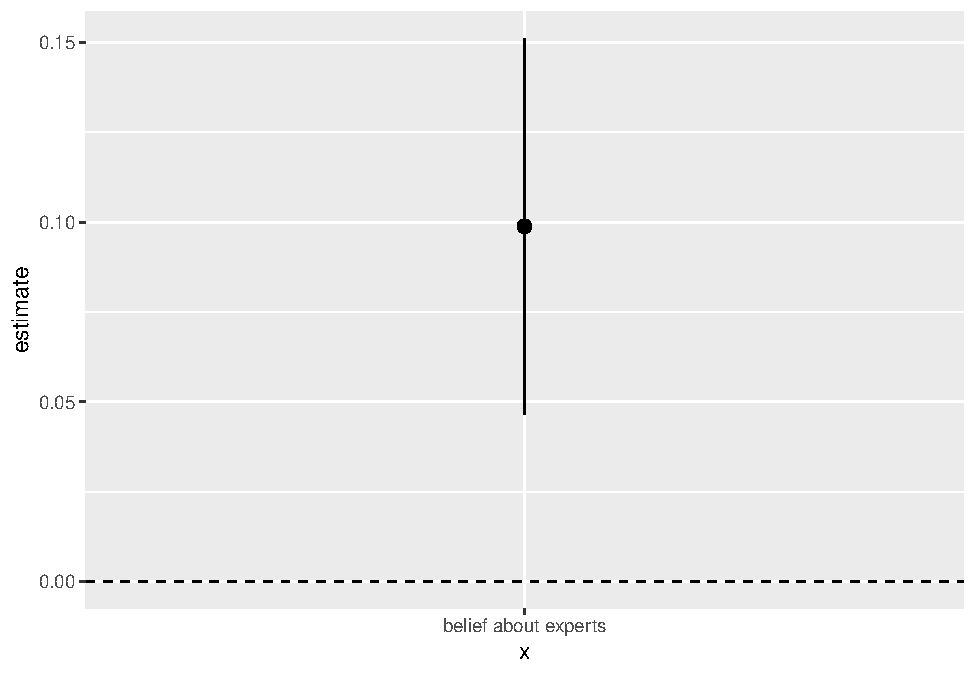
\includegraphics[keepaspectratio]{POL342-tutorial-notes_files/figure-latex/unnamed-chunk-158-1.pdf}}

\subsubsection*{\texorpdfstring{To beautify the graph, we might change its \texttt{theme} and change x and y labels (\texttt{xlab} and \texttt{ylab}).}{To beautify the graph, we might change its theme and change x and y labels (xlab and ylab).}}\label{to-beautify-the-graph-we-might-change-its-theme-and-change-x-and-y-labels-xlab-and-ylab.}
\addcontentsline{toc}{subsubsection}{To beautify the graph, we might change its \texttt{theme} and change x and y labels (\texttt{xlab} and \texttt{ylab}).}

\begin{Shaded}
\begin{Highlighting}[]
\FunctionTok{t.test}\NormalTok{(accuracy }\SpecialCharTok{\textasciitilde{}} \FunctionTok{factor}\NormalTok{(treated, }\AttributeTok{levels=}\FunctionTok{c}\NormalTok{(}\DecValTok{1}\NormalTok{,}\DecValTok{0}\NormalTok{)), }\AttributeTok{data =}\NormalTok{ df) }\SpecialCharTok{|\textgreater{}}
  \FunctionTok{tidy}\NormalTok{() }\SpecialCharTok{|\textgreater{}}
  \FunctionTok{ggplot}\NormalTok{(}\FunctionTok{aes}\NormalTok{(}\AttributeTok{y=}\NormalTok{estimate,}\AttributeTok{x=}\StringTok{"belief about experts"}\NormalTok{)) }\SpecialCharTok{+} 
  \FunctionTok{geom\_pointrange}\NormalTok{(}\FunctionTok{aes}\NormalTok{(}\AttributeTok{ymax=}\NormalTok{conf.high,}\AttributeTok{ymin=}\NormalTok{conf.low)) }\SpecialCharTok{+}
  \FunctionTok{geom\_hline}\NormalTok{(}\FunctionTok{aes}\NormalTok{(}\AttributeTok{yintercept=}\DecValTok{0}\NormalTok{),}\AttributeTok{linetype=}\StringTok{"dashed"}\NormalTok{) }\SpecialCharTok{+}
  \FunctionTok{theme\_bw}\NormalTok{() }\SpecialCharTok{+} \CommentTok{\# black and white theme}
  \FunctionTok{xlab}\NormalTok{(}\StringTok{""}\NormalTok{) }\SpecialCharTok{+} \CommentTok{\# hides the x label}
  \FunctionTok{ylab}\NormalTok{(}\StringTok{"Difference in means"}\NormalTok{) }\CommentTok{\# replaces the y label}
\end{Highlighting}
\end{Shaded}

\pandocbounded{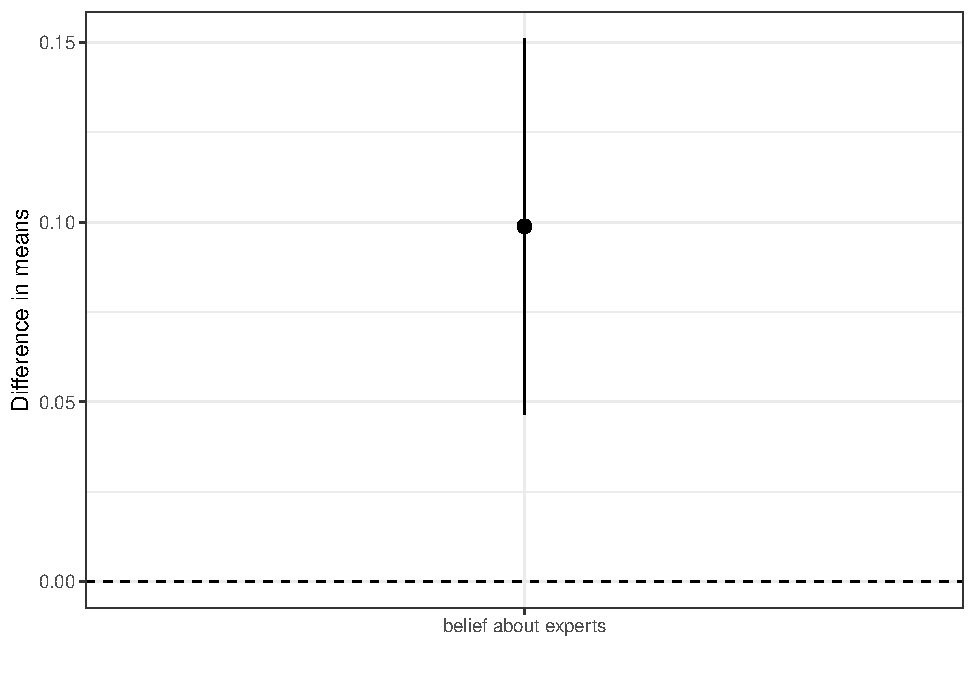
\includegraphics[keepaspectratio]{POL342-tutorial-notes_files/figure-latex/unnamed-chunk-159-1.pdf}}

\begin{Shaded}
\begin{Highlighting}[]
\FunctionTok{t.test}\NormalTok{(preference }\SpecialCharTok{\textasciitilde{}} \FunctionTok{factor}\NormalTok{(treated, }\AttributeTok{levels=}\FunctionTok{c}\NormalTok{(}\DecValTok{1}\NormalTok{,}\DecValTok{0}\NormalTok{)), }\AttributeTok{data =}\NormalTok{ df) }\SpecialCharTok{|\textgreater{}}
  \FunctionTok{tidy}\NormalTok{() }\SpecialCharTok{|\textgreater{}}
  \FunctionTok{ggplot}\NormalTok{(}\FunctionTok{aes}\NormalTok{(}\AttributeTok{y=}\NormalTok{estimate,}\AttributeTok{x=}\StringTok{"policy preference"}\NormalTok{)) }\SpecialCharTok{+} 
  \FunctionTok{geom\_pointrange}\NormalTok{(}\FunctionTok{aes}\NormalTok{(}\AttributeTok{ymax=}\NormalTok{conf.high,}\AttributeTok{ymin=}\NormalTok{conf.low)) }\SpecialCharTok{+}
  \FunctionTok{geom\_hline}\NormalTok{(}\FunctionTok{aes}\NormalTok{(}\AttributeTok{yintercept=}\DecValTok{0}\NormalTok{),}\AttributeTok{linetype=}\StringTok{"dashed"}\NormalTok{) }\SpecialCharTok{+}
  \FunctionTok{theme\_bw}\NormalTok{() }\SpecialCharTok{+}
  \FunctionTok{xlab}\NormalTok{(}\StringTok{""}\NormalTok{) }\SpecialCharTok{+}
  \FunctionTok{ylab}\NormalTok{(}\StringTok{"Difference in means"}\NormalTok{)}
\end{Highlighting}
\end{Shaded}

\pandocbounded{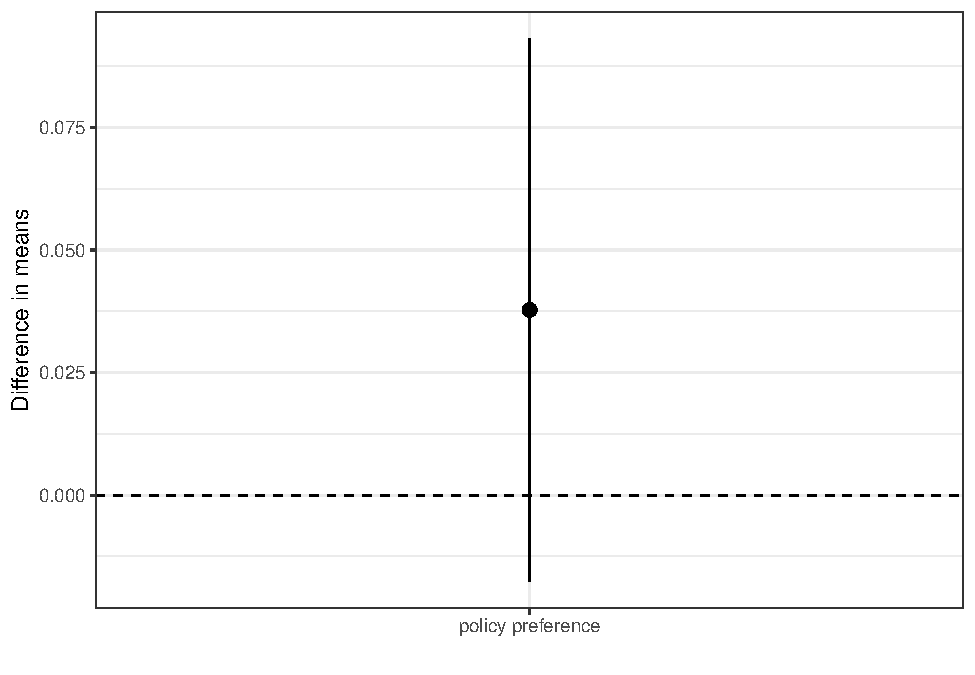
\includegraphics[keepaspectratio]{POL342-tutorial-notes_files/figure-latex/unnamed-chunk-160-1.pdf}}

You could also flip the x and y.

\begin{Shaded}
\begin{Highlighting}[]
\FunctionTok{t.test}\NormalTok{(preference }\SpecialCharTok{\textasciitilde{}} \FunctionTok{factor}\NormalTok{(treated, }\AttributeTok{levels=}\FunctionTok{c}\NormalTok{(}\DecValTok{1}\NormalTok{,}\DecValTok{0}\NormalTok{)), }\AttributeTok{data =}\NormalTok{ df) }\SpecialCharTok{|\textgreater{}}
  \FunctionTok{tidy}\NormalTok{() }\SpecialCharTok{|\textgreater{}}
  \FunctionTok{ggplot}\NormalTok{(}\FunctionTok{aes}\NormalTok{(}\AttributeTok{x=}\NormalTok{estimate,}\AttributeTok{y=}\StringTok{"policy preference"}\NormalTok{)) }\SpecialCharTok{+} 
  \FunctionTok{geom\_pointrange}\NormalTok{(}\FunctionTok{aes}\NormalTok{(}\AttributeTok{xmax=}\NormalTok{conf.high,}\AttributeTok{xmin=}\NormalTok{conf.low)) }\SpecialCharTok{+}
  \FunctionTok{geom\_vline}\NormalTok{(}\FunctionTok{aes}\NormalTok{(}\AttributeTok{xintercept=}\DecValTok{0}\NormalTok{),}\AttributeTok{linetype=}\StringTok{"dashed"}\NormalTok{) }\SpecialCharTok{+}
  \FunctionTok{theme\_bw}\NormalTok{() }\SpecialCharTok{+}
  \FunctionTok{ylab}\NormalTok{(}\StringTok{""}\NormalTok{) }\SpecialCharTok{+}
  \FunctionTok{xlab}\NormalTok{(}\StringTok{"Difference in means"}\NormalTok{)}
\end{Highlighting}
\end{Shaded}

\pandocbounded{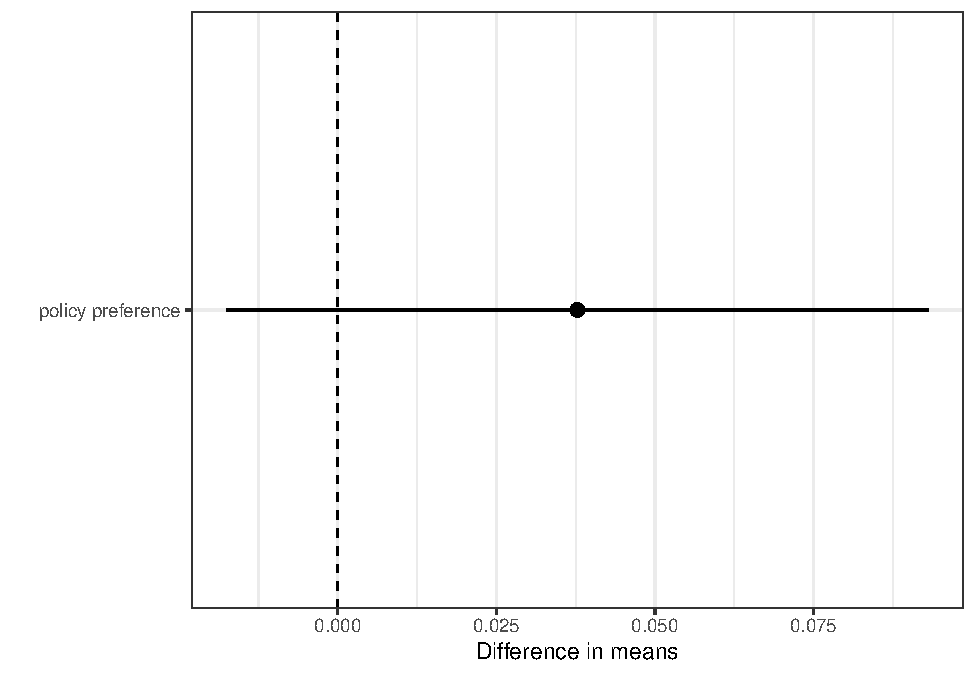
\includegraphics[keepaspectratio]{POL342-tutorial-notes_files/figure-latex/unnamed-chunk-161-1.pdf}}

\section{Linear regression}\label{linear-regression}

\subsection*{Load a different dataset (some variables from Varieties of Democracies data set)}\label{load-a-different-dataset-some-variables-from-varieties-of-democracies-data-set}
\addcontentsline{toc}{subsection}{Load a different dataset (some variables from Varieties of Democracies data set)}

\begin{Shaded}
\begin{Highlighting}[]
\NormalTok{d }\OtherTok{\textless{}{-}} \FunctionTok{read.csv}\NormalTok{(}\StringTok{"vdem\_w6tutorial.csv"}\NormalTok{)}
\end{Highlighting}
\end{Shaded}

\begin{itemize}
\tightlist
\item
  Variables from Varieties of Democracy dataset

  \begin{itemize}
  \tightlist
  \item
    Power distributed by gender (C) (v2pepwrgen): Q. Is political power distributed according to gender? (0: Men have a near-monopoly power on political power, 4: Men and women have roughly equal political power.)
  \item
    Female journalists (C) (v2mefemjrn): Q. Please estimate the percentage (\%) of journalists in the print and broadcast media who are women. (Interval)
  \end{itemize}
\end{itemize}

\subsection*{V-Dem codebook}\label{v-dem-codebook}
\addcontentsline{toc}{subsection}{V-Dem codebook}

\begin{center}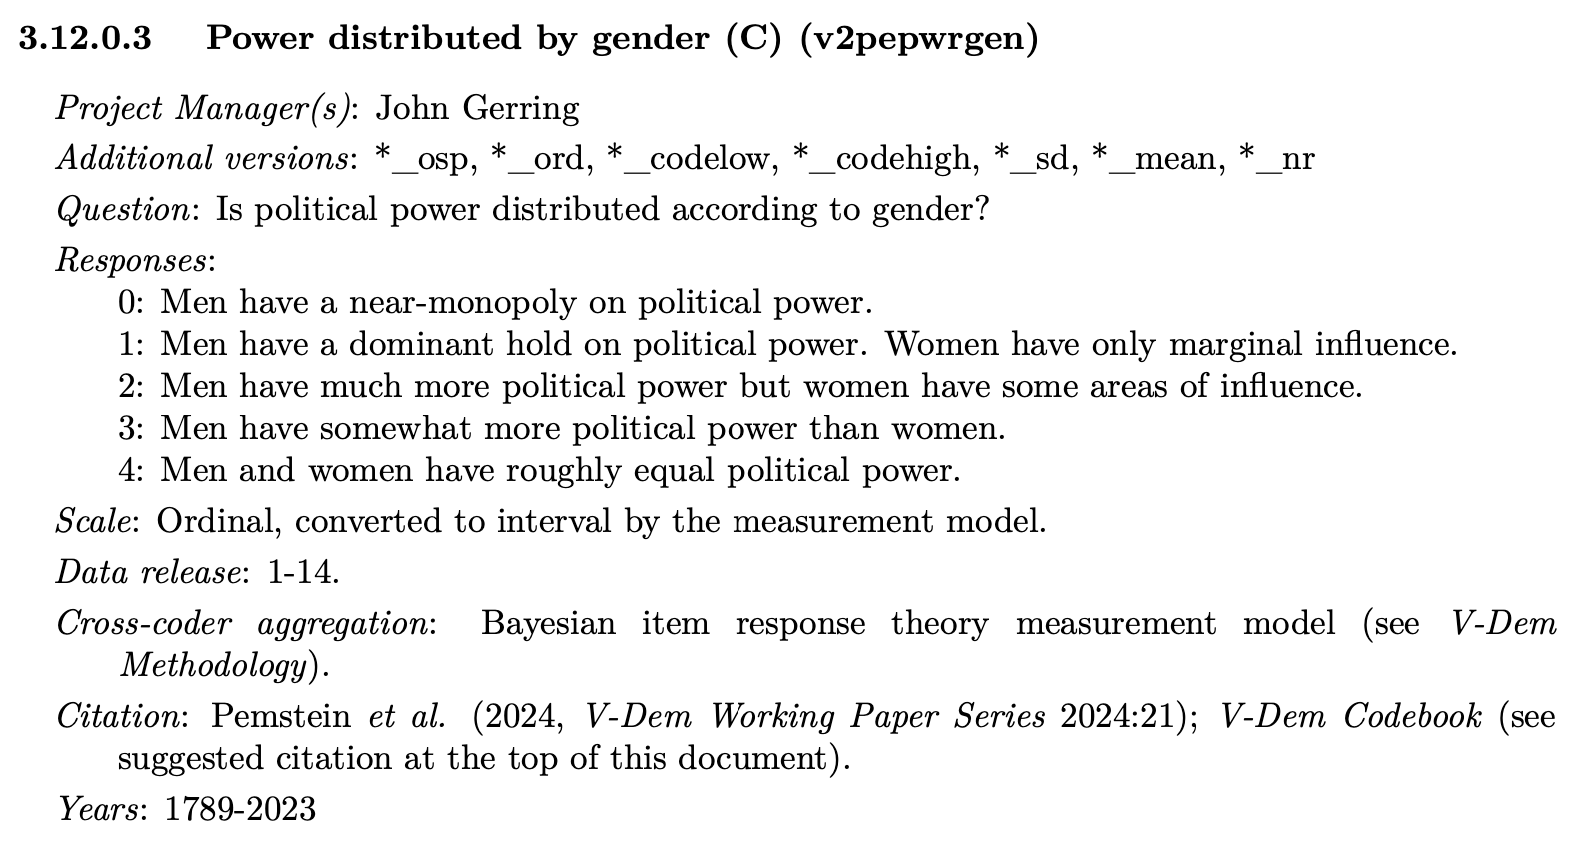
\includegraphics[width=0.7\linewidth]{images/w6_vdemcodebook} \end{center}

More details on codebook next week!

\begin{Shaded}
\begin{Highlighting}[]
\FunctionTok{summary}\NormalTok{(d}\SpecialCharTok{$}\NormalTok{v2pepwrgen)}
\end{Highlighting}
\end{Shaded}

\begin{verbatim}
##    Min. 1st Qu.  Median    Mean 3rd Qu.    Max. 
## -2.8170  0.3645  1.0180  0.9792  1.6885  3.7120
\end{verbatim}

\subsection*{\texorpdfstring{Bivariate relationship using a scatter plot \texttt{geom\_point()}}{Bivariate relationship using a scatter plot geom\_point()}}\label{bivariate-relationship-using-a-scatter-plot-geom_point}
\addcontentsline{toc}{subsection}{Bivariate relationship using a scatter plot \texttt{geom\_point()}}

\begin{Shaded}
\begin{Highlighting}[]
\NormalTok{d }\SpecialCharTok{|\textgreater{}}
  \FunctionTok{ggplot}\NormalTok{(}\FunctionTok{aes}\NormalTok{(}\AttributeTok{y=}\NormalTok{v2pepwrgen,}\AttributeTok{x=}\NormalTok{v2mefemjrn)) }\SpecialCharTok{+}
  \FunctionTok{geom\_point}\NormalTok{() }\SpecialCharTok{+}
  \FunctionTok{theme\_classic}\NormalTok{()}
\end{Highlighting}
\end{Shaded}

\pandocbounded{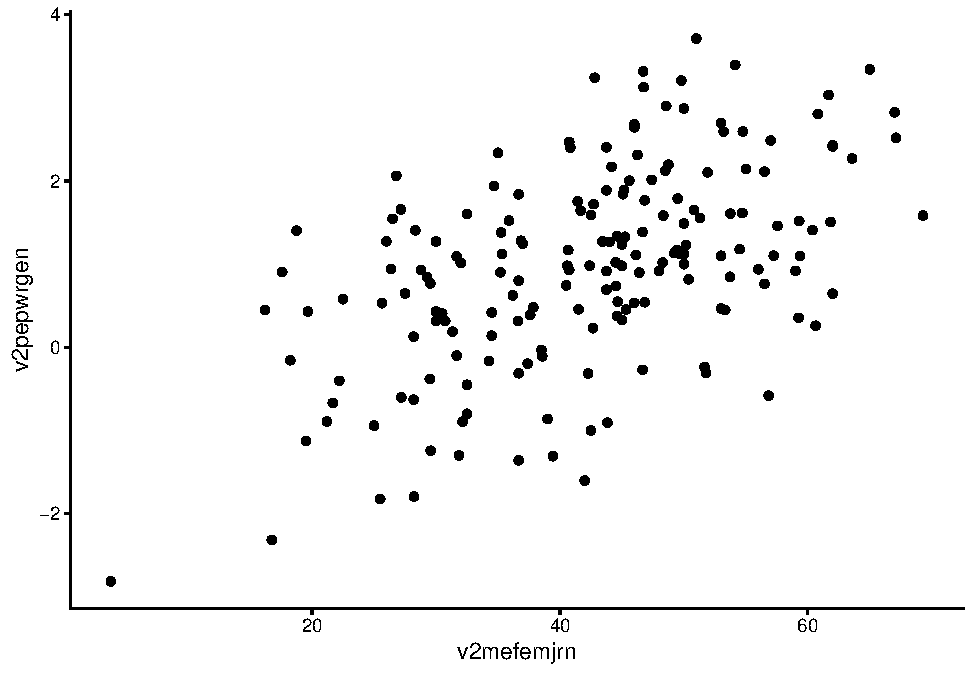
\includegraphics[keepaspectratio]{POL342-tutorial-notes_files/figure-latex/unnamed-chunk-166-1.pdf}}

\pandocbounded{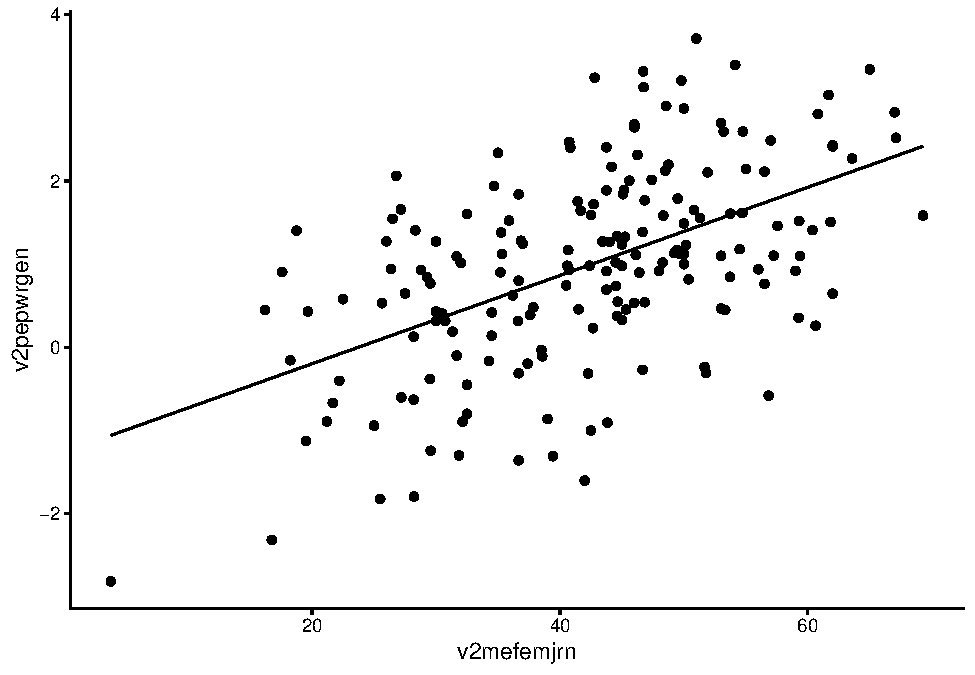
\includegraphics[keepaspectratio]{POL342-tutorial-notes_files/figure-latex/unnamed-chunk-167-1.pdf}}

\pandocbounded{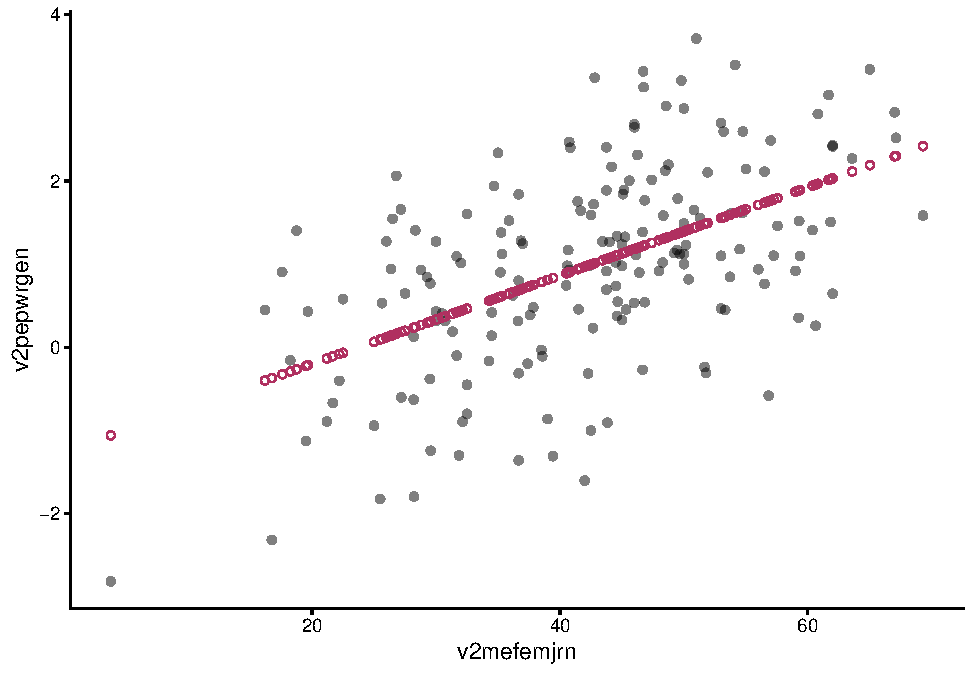
\includegraphics[keepaspectratio]{POL342-tutorial-notes_files/figure-latex/unnamed-chunk-168-1.pdf}}

\pandocbounded{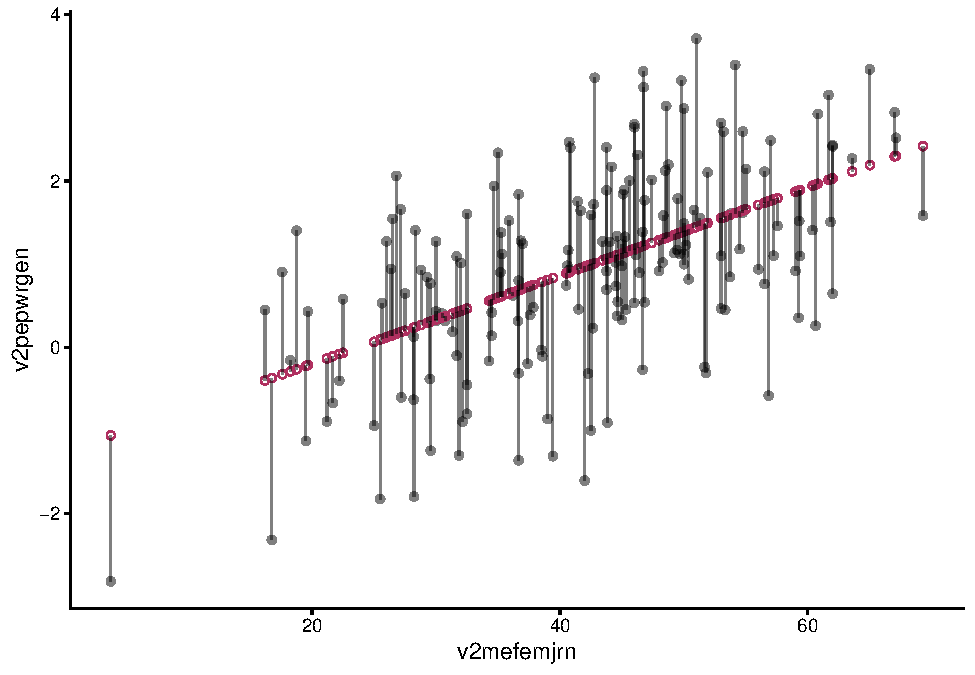
\includegraphics[keepaspectratio]{POL342-tutorial-notes_files/figure-latex/unnamed-chunk-169-1.pdf}}

\pandocbounded{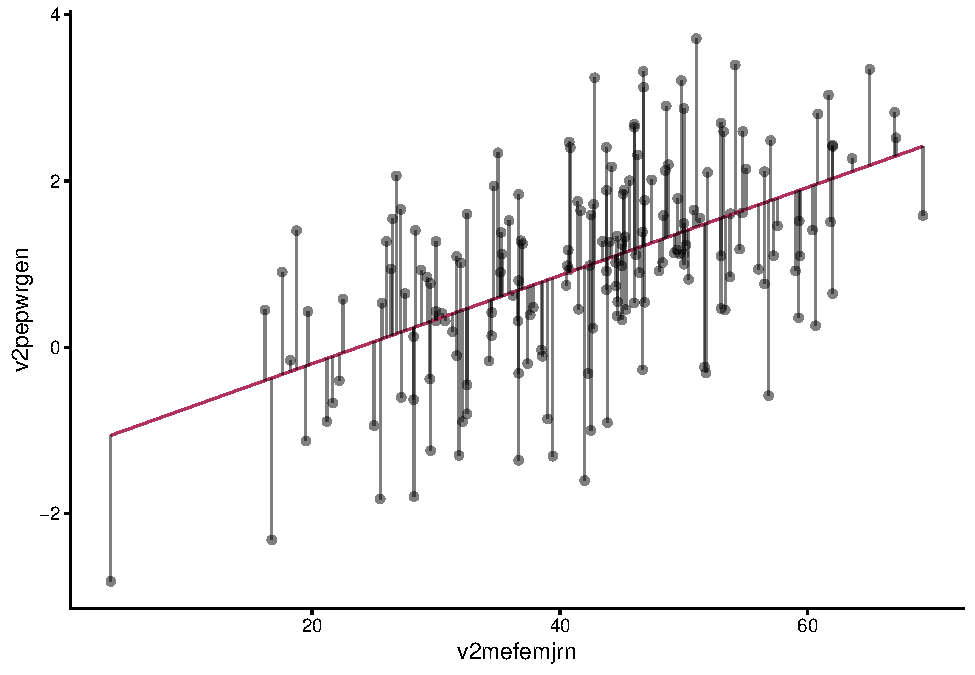
\includegraphics[keepaspectratio]{POL342-tutorial-notes_files/figure-latex/unnamed-chunk-170-1.pdf}}

\subsubsection*{Regression output}\label{regression-output}
\addcontentsline{toc}{subsubsection}{Regression output}

\subsubsection*{\texorpdfstring{Visualizing regression line using \texttt{geom\_smooth()}}{Visualizing regression line using geom\_smooth()}}\label{visualizing-regression-line-using-geom_smooth}
\addcontentsline{toc}{subsubsection}{Visualizing regression line using \texttt{geom\_smooth()}}

\begin{Shaded}
\begin{Highlighting}[]
\NormalTok{d }\SpecialCharTok{|\textgreater{}}
  \FunctionTok{ggplot}\NormalTok{(}\FunctionTok{aes}\NormalTok{(}\AttributeTok{y=}\NormalTok{v2pepwrgen,}\AttributeTok{x=}\NormalTok{v2mefemjrn)) }\SpecialCharTok{+}
  \FunctionTok{geom\_point}\NormalTok{(}\AttributeTok{alpha=}\FloatTok{0.5}\NormalTok{) }\SpecialCharTok{+} \CommentTok{\# alpha changes the transparency of the points}
  \FunctionTok{geom\_smooth}\NormalTok{(}\AttributeTok{method=}\StringTok{"lm"}\NormalTok{) }\SpecialCharTok{+}
  \FunctionTok{theme\_classic}\NormalTok{()}
\end{Highlighting}
\end{Shaded}

\pandocbounded{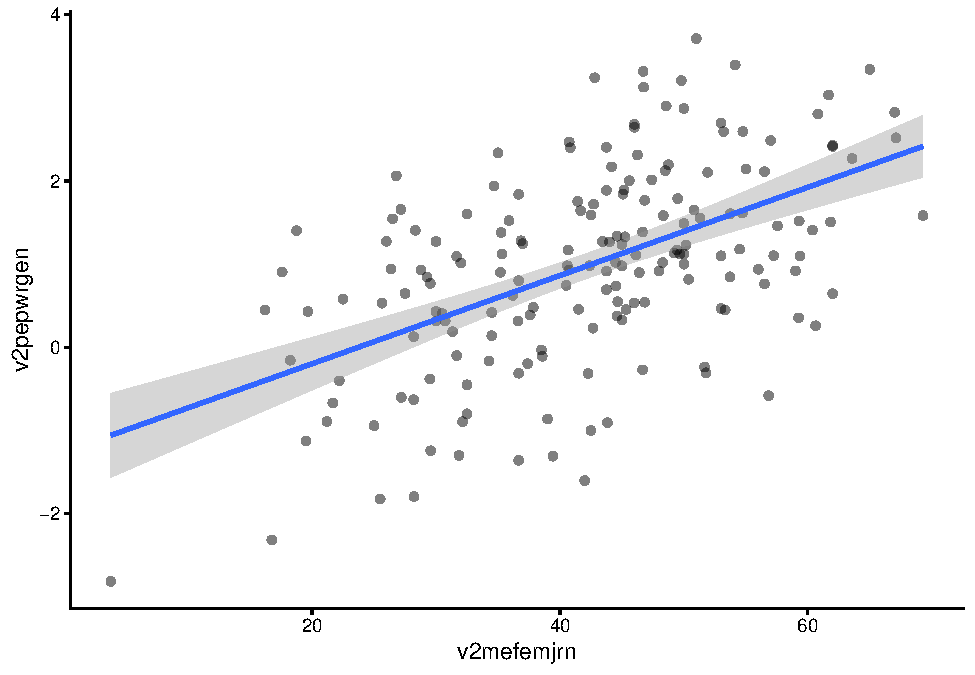
\includegraphics[keepaspectratio]{POL342-tutorial-notes_files/figure-latex/unnamed-chunk-171-1.pdf}}

\subsection*{Regression estimates (similar to survey treatment visualization)}\label{regression-estimates-similar-to-survey-treatment-visualization}
\addcontentsline{toc}{subsection}{Regression estimates (similar to survey treatment visualization)}

\begin{Shaded}
\begin{Highlighting}[]
\FunctionTok{lm}\NormalTok{(}\AttributeTok{data=}\NormalTok{d,v2pepwrgen }\SpecialCharTok{\textasciitilde{}}\NormalTok{ v2mefemjrn) }\SpecialCharTok{|\textgreater{}}
  \FunctionTok{tidy}\NormalTok{(}\AttributeTok{conf.int=}\NormalTok{T,}\AttributeTok{conf.level=}\NormalTok{.}\DecValTok{95}\NormalTok{) }\SpecialCharTok{|\textgreater{}}
  \FunctionTok{filter}\NormalTok{(term}\SpecialCharTok{!=}\StringTok{"(Intercept)"}\NormalTok{) }\SpecialCharTok{|\textgreater{}}
  \FunctionTok{ggplot}\NormalTok{(}\FunctionTok{aes}\NormalTok{(}\AttributeTok{y=}\NormalTok{estimate,}\AttributeTok{x=}\StringTok{"\% Female Journalists"}\NormalTok{)) }\SpecialCharTok{+} 
  \FunctionTok{geom\_pointrange}\NormalTok{(}\FunctionTok{aes}\NormalTok{(}\AttributeTok{ymax=}\NormalTok{conf.high,}\AttributeTok{ymin=}\NormalTok{conf.low,)) }\SpecialCharTok{+}
  \FunctionTok{geom\_hline}\NormalTok{(}\FunctionTok{aes}\NormalTok{(}\AttributeTok{yintercept=}\DecValTok{0}\NormalTok{),}\AttributeTok{linetype=}\StringTok{"dashed"}\NormalTok{) }\SpecialCharTok{+}
  \FunctionTok{theme\_bw}\NormalTok{() }\SpecialCharTok{+}
  \FunctionTok{ylab}\NormalTok{(}\StringTok{"Coefficient Estimate"}\NormalTok{) }\SpecialCharTok{+}
  \FunctionTok{xlab}\NormalTok{(}\StringTok{""}\NormalTok{)}
\end{Highlighting}
\end{Shaded}

\pandocbounded{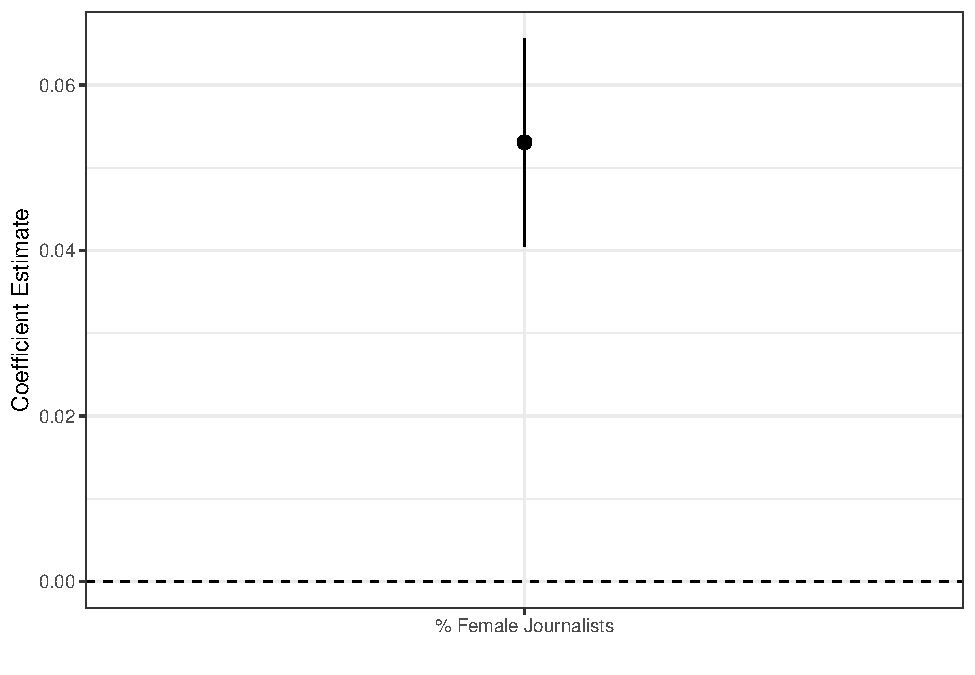
\includegraphics[keepaspectratio]{POL342-tutorial-notes_files/figure-latex/unnamed-chunk-172-1.pdf}}

\section{Credits}\label{credits-3}

\begin{itemize}
\tightlist
\item
  This lesson includes materials from

  \begin{itemize}
  \tightlist
  \item
    \href{https://github.com/dgrtwo/unvotes}{unvotes}
  \end{itemize}
\end{itemize}

\chapter{Introducing project datasets}\label{introducing-project-datasets}

\begin{itemize}
\tightlist
\item
  Goals for today's class:

  \begin{itemize}
  \tightlist
  \item
    Learning to use the project datasets

    \begin{itemize}
    \tightlist
    \item
      Varieties of Democracy (VDem)
    \item
      Canadian Election Study 2021
    \item
      World Values Survey (Wave 7)
    \item
      Asian Barometer (Wave 5)
    \end{itemize}
  \end{itemize}
\end{itemize}

\section{Set-up}\label{set-up}

\subsection*{Download project datasets}\label{download-project-datasets}
\addcontentsline{toc}{subsection}{Download project datasets}

This will take a while because the files are large.

\begin{center}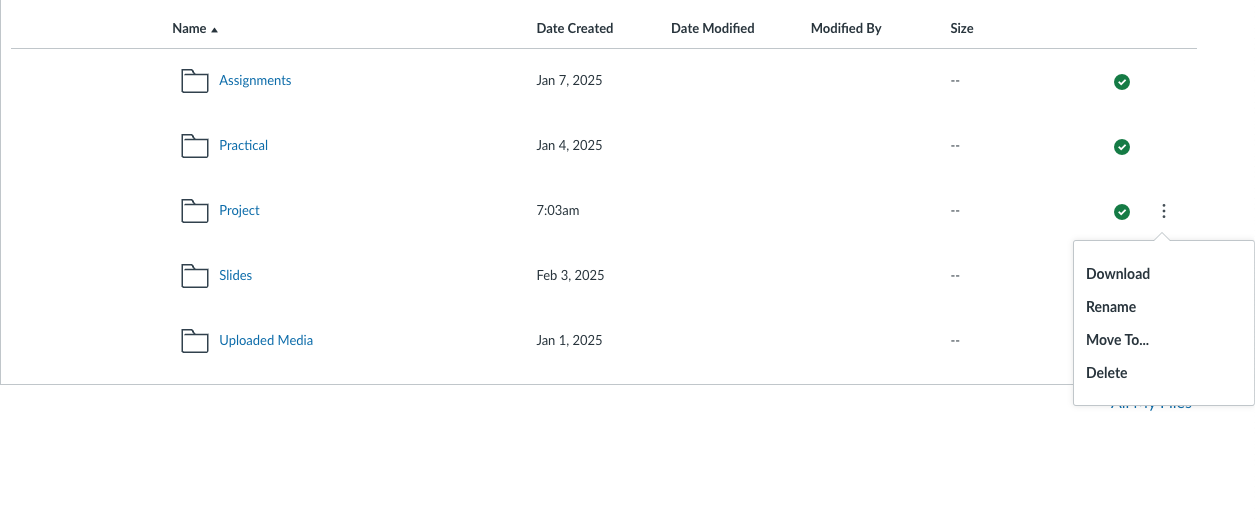
\includegraphics[width=1\linewidth]{images/w7_projectdata} \end{center}

\subsection*{\texorpdfstring{Download the other file (\texttt{W8.R}) and put everything in your R project folder}{Download the other file (W8.R) and put everything in your R project folder}}\label{download-the-other-file-w8.r-and-put-everything-in-your-r-project-folder}
\addcontentsline{toc}{subsection}{Download the other file (\texttt{W8.R}) and put everything in your R project folder}

\begin{center}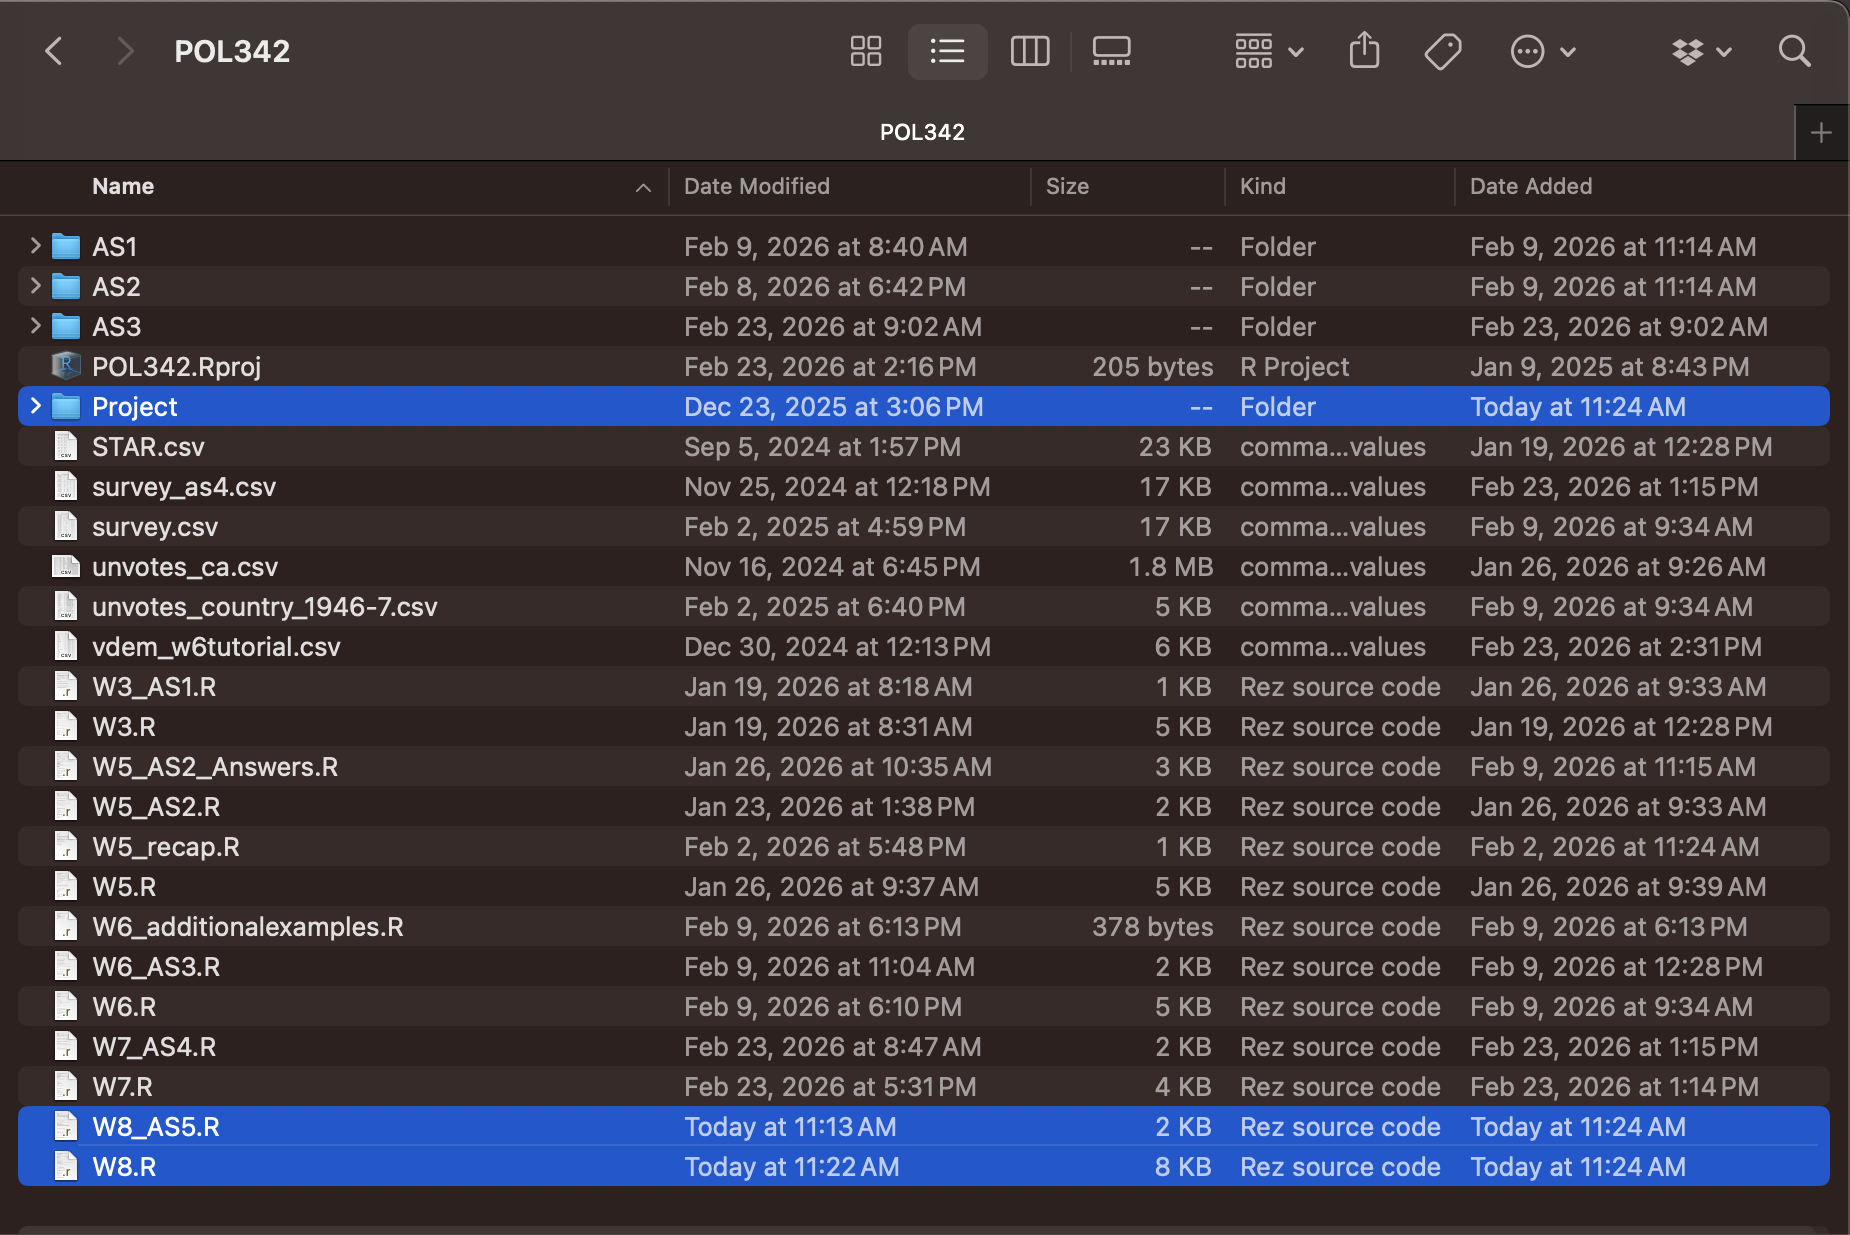
\includegraphics[width=1\linewidth]{images/W7} \end{center}

\subsection*{Load libraries}\label{load-libraries}
\addcontentsline{toc}{subsection}{Load libraries}

\subsubsection*{Install package ``haven''}\label{install-package-haven}
\addcontentsline{toc}{subsubsection}{Install package ``haven''}

\begin{Shaded}
\begin{Highlighting}[]
\FunctionTok{library}\NormalTok{(tidyverse)}
\FunctionTok{library}\NormalTok{(sjPlot)}

\FunctionTok{install.packages}\NormalTok{(}\StringTok{"haven"}\NormalTok{)}
\FunctionTok{library}\NormalTok{(haven) }\CommentTok{\# to read Stata .dta files}
\end{Highlighting}
\end{Shaded}

\section{Overview: Use of data sets}\label{overview-use-of-data-sets}

This is the general approach we will take to use the datasets for the project assignment.

\subsection*{Step 1: Select one of the four data sets}\label{step-1-select-one-of-the-four-data-sets}
\addcontentsline{toc}{subsection}{Step 1: Select one of the four data sets}

Each data set focuses on a different type of data. You will be selecting variables from \emph{one dataset} for your term project. Take a look at the code book and decide which data set you want to use.

\subsection*{Step 2: Select your variables}\label{step-2-select-your-variables}
\addcontentsline{toc}{subsection}{Step 2: Select your variables}

Look at the \textbf{codebook} to find your variables.

\subsection*{Step 3: Trim down the data set}\label{step-3-trim-down-the-data-set}
\addcontentsline{toc}{subsection}{Step 3: Trim down the data set}

Before examining the variables, it is helpful to trim down your data set to the variables you have selected.

\subsubsection*{Additional step:}\label{additional-step}
\addcontentsline{toc}{subsubsection}{Additional step:}

\begin{itemize}
\tightlist
\item
  For the following data sets, you have to select a subset of the data

  \begin{itemize}
  \tightlist
  \item
    VDem: Select a year (from year 2000 onwards)
  \item
    World Values Survey: Select one country
  \item
    Asian Barometer: Select one country
  \end{itemize}
\end{itemize}

\subsection*{Step 4: Examine the univariate distribution and bivariate relationship}\label{step-4-examine-the-univariate-distribution-and-bivariate-relationship}
\addcontentsline{toc}{subsection}{Step 4: Examine the univariate distribution and bivariate relationship}

\section{VDem}\label{vdem}

Look at the codebook, which can be found in the same folder as the dataset.

\subsection*{Step 2: Select your variables}\label{step-2-select-your-variables-1}
\addcontentsline{toc}{subsection}{Step 2: Select your variables}

Select the variables you want and assign them to the variable \texttt{vars}. I've selected\\

\begin{itemize}
\tightlist
\item
  Country name
\item
  Country ID
\item
  Year
\item
  \textbf{Political corruption index (v2x\_corr)}
\item
  \textbf{GDPpercapita (e\_gdppc)}
\end{itemize}

\begin{Shaded}
\begin{Highlighting}[]
\NormalTok{vars }\OtherTok{\textless{}{-}} \FunctionTok{c}\NormalTok{(}\StringTok{"country\_name"}\NormalTok{, }\StringTok{"country\_id"}\NormalTok{, }\StringTok{"year"}\NormalTok{, }
          \StringTok{"v2x\_corr"}\NormalTok{,}\StringTok{"e\_gdppc"}\NormalTok{)}
\end{Highlighting}
\end{Shaded}

\begin{center}\includegraphics[width=1\linewidth]{images/W7_gdppc} \end{center}

\begin{center}\includegraphics[width=1\linewidth]{images/W7_corr} \end{center}

\begin{center}\includegraphics[width=1\linewidth]{images/W7_corr2} \end{center}

\subsection*{Step 3: Trim down the data set (select a year)}\label{step-3-trim-down-the-data-set-select-a-year}
\addcontentsline{toc}{subsection}{Step 3: Trim down the data set (select a year)}

Select a year for analysis and use the \texttt{filter} function to extract the data for that year. Please note that the VDem file in your project folder is a reduced version of the original dataset. You can find the original dataset \href{https://www.v-dem.net/data/the-v-dem-dataset/}{here}.

\begin{Shaded}
\begin{Highlighting}[]
\NormalTok{vdem\_selected }\OtherTok{\textless{}{-}} \FunctionTok{read.csv}\NormalTok{(}\StringTok{"Project/VDem/VDem\_post2000.csv"}\NormalTok{) }\SpecialCharTok{|\textgreater{}}
  \FunctionTok{select}\NormalTok{(vars) }\SpecialCharTok{|\textgreater{}}
  \FunctionTok{filter}\NormalTok{(year}\SpecialCharTok{==}\DecValTok{2019}\NormalTok{)}
\end{Highlighting}
\end{Shaded}

\subsection*{Step 4: Examine the univariate distribution and bivariate relationship}\label{step-4-examine-the-univariate-distribution-and-bivariate-relationship-1}
\addcontentsline{toc}{subsection}{Step 4: Examine the univariate distribution and bivariate relationship}

\subsubsection*{Look at the summary statistics}\label{look-at-the-summary-statistics}
\addcontentsline{toc}{subsubsection}{Look at the summary statistics}

\begin{Shaded}
\begin{Highlighting}[]
\FunctionTok{summary}\NormalTok{(vdem\_selected)}
\end{Highlighting}
\end{Shaded}

\begin{verbatim}
##  country_name         country_id          year         v2x_corr     
##  Length:179         Min.   :  3.00   Min.   :2019   Min.   :0.0020  
##  Class :character   1st Qu.: 51.50   1st Qu.:2019   1st Qu.:0.2190  
##  Mode  :character   Median : 96.00   Median :2019   Median :0.5300  
##                     Mean   : 99.12   Mean   :2019   Mean   :0.4906  
##                     3rd Qu.:145.00   3rd Qu.:2019   3rd Qu.:0.7475  
##                     Max.   :236.00   Max.   :2019   Max.   :0.9560  
##                                                                     
##     e_gdppc      
##  Min.   : 0.735  
##  1st Qu.: 4.060  
##  Median :11.017  
##  Mean   :17.827  
##  3rd Qu.:25.777  
##  Max.   :92.389  
##  NA's   :5
\end{verbatim}

\subsubsection*{Univariate: Examine each variable}\label{univariate-examine-each-variable}
\addcontentsline{toc}{subsubsection}{Univariate: Examine each variable}

I am going to plot histograms because both of the variables are continuous numerical measures. If you choose a categorical variable, you would visualize the univariate distribution using a bar chart.

\begin{Shaded}
\begin{Highlighting}[]
\FunctionTok{ggplot}\NormalTok{(vdem\_selected,}\FunctionTok{aes}\NormalTok{(}\AttributeTok{x=}\NormalTok{v2x\_corr)) }\SpecialCharTok{+}
  \FunctionTok{geom\_histogram}\NormalTok{()}
\end{Highlighting}
\end{Shaded}

\pandocbounded{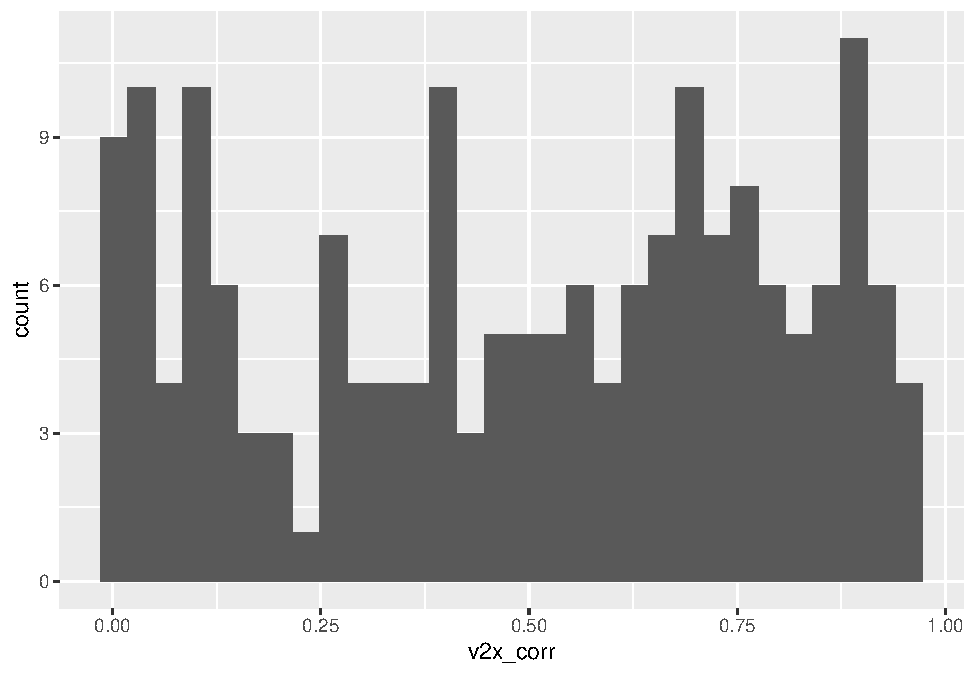
\includegraphics[keepaspectratio]{POL342-tutorial-notes_files/figure-latex/unnamed-chunk-183-1.pdf}}

\subsubsection{GDP per capita is measured in 10,000 PPP-adjusted dollars.}\label{gdp-per-capita-is-measured-in-10000-ppp-adjusted-dollars.}

\begin{Shaded}
\begin{Highlighting}[]
\FunctionTok{ggplot}\NormalTok{(vdem\_selected,}\FunctionTok{aes}\NormalTok{(}\AttributeTok{x=}\NormalTok{e\_gdppc)) }\SpecialCharTok{+}
  \FunctionTok{geom\_histogram}\NormalTok{()}
\end{Highlighting}
\end{Shaded}

\pandocbounded{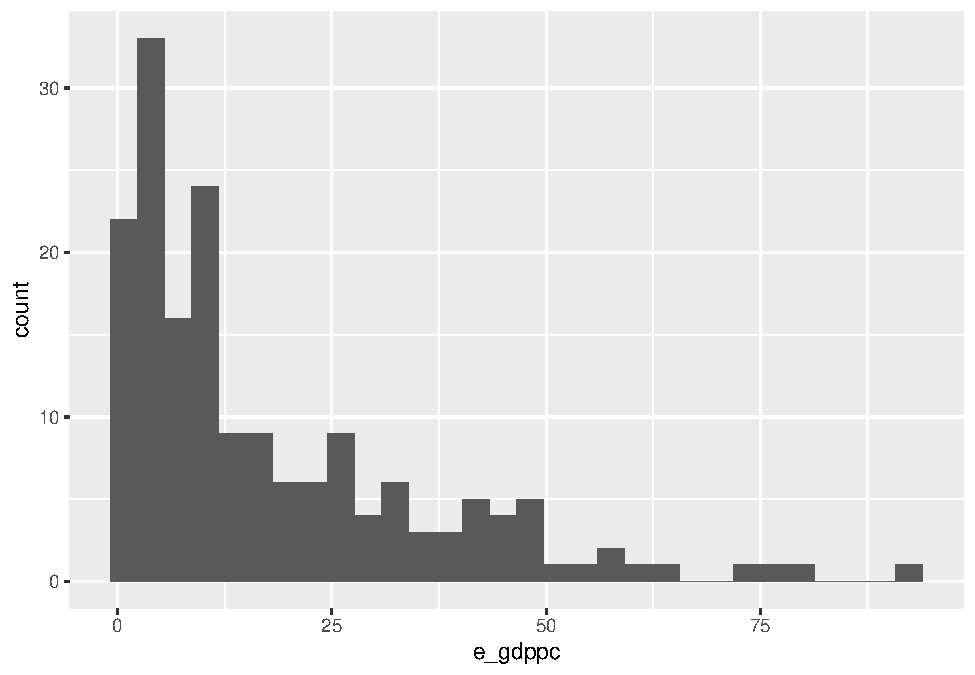
\includegraphics[keepaspectratio]{POL342-tutorial-notes_files/figure-latex/unnamed-chunk-184-1.pdf}}

\subsubsection*{Bivariate relationship}\label{bivariate-relationship}
\addcontentsline{toc}{subsubsection}{Bivariate relationship}

A scatter plot is selected here because both variables are continuuous numerical measures.

\begin{Shaded}
\begin{Highlighting}[]
\FunctionTok{ggplot}\NormalTok{(}\AttributeTok{data=}\NormalTok{vdem\_selected,}\FunctionTok{aes}\NormalTok{(}\AttributeTok{x=}\NormalTok{v2x\_corr,}\AttributeTok{y=}\NormalTok{e\_gdppc)) }\SpecialCharTok{+}
  \FunctionTok{geom\_point}\NormalTok{()}
\end{Highlighting}
\end{Shaded}

\pandocbounded{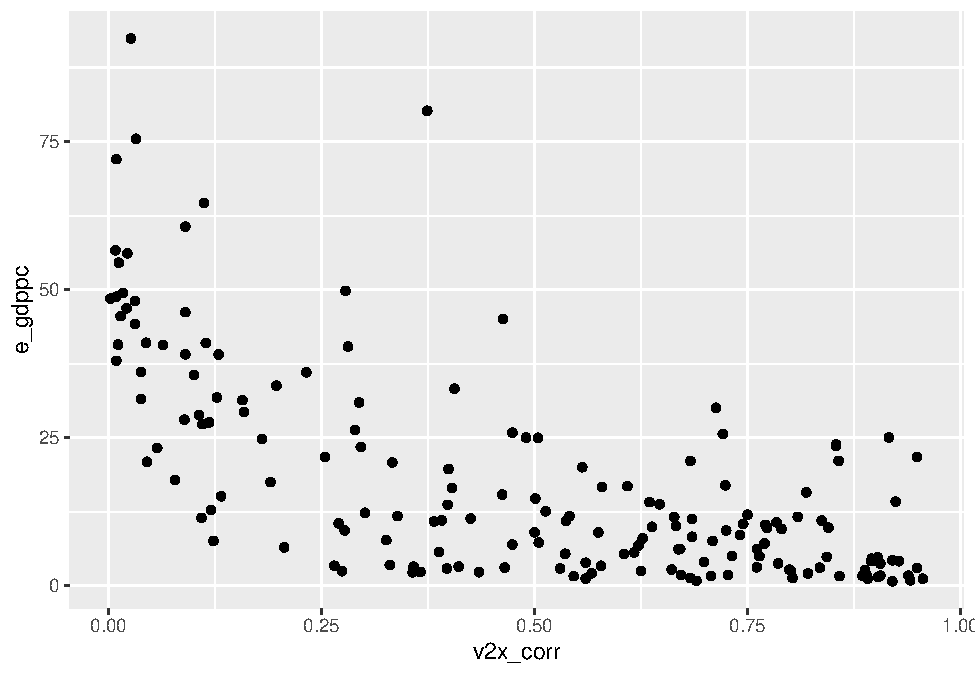
\includegraphics[keepaspectratio]{POL342-tutorial-notes_files/figure-latex/unnamed-chunk-185-1.pdf}}

\subsubsection*{Change the theme and transparency of points}\label{change-the-theme-and-transparency-of-points}
\addcontentsline{toc}{subsubsection}{Change the theme and transparency of points}

\begin{Shaded}
\begin{Highlighting}[]
\FunctionTok{ggplot}\NormalTok{(}\AttributeTok{data=}\NormalTok{vdem\_selected,}\FunctionTok{aes}\NormalTok{(}\AttributeTok{x=}\NormalTok{v2x\_corr,}\AttributeTok{y=}\NormalTok{e\_gdppc)) }\SpecialCharTok{+}
  \FunctionTok{geom\_point}\NormalTok{(}\AttributeTok{alpha=}\NormalTok{.}\DecValTok{5}\NormalTok{) }\SpecialCharTok{+}
  \FunctionTok{theme\_bw}\NormalTok{()}
\end{Highlighting}
\end{Shaded}

\pandocbounded{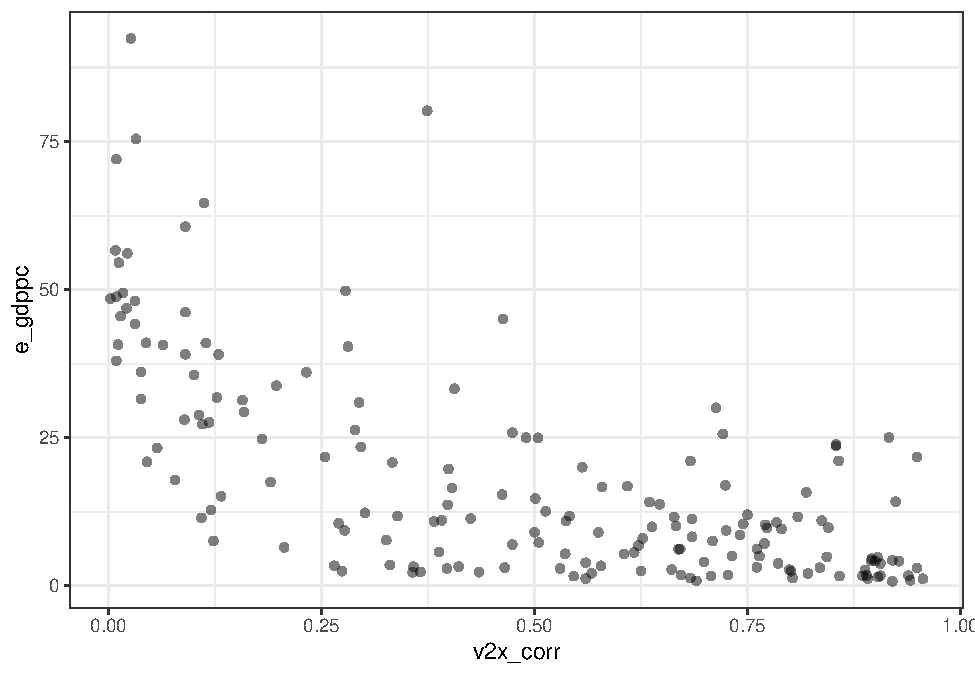
\includegraphics[keepaspectratio]{POL342-tutorial-notes_files/figure-latex/unnamed-chunk-186-1.pdf}}

\subsection*{Remove all from environment}\label{remove-all-from-environment}
\addcontentsline{toc}{subsection}{Remove all from environment}

To avoid any misspecification of variables, clear environment before moving on to the next dataset.

\begin{Shaded}
\begin{Highlighting}[]
\FunctionTok{rm}\NormalTok{(}\AttributeTok{list=}\FunctionTok{ls}\NormalTok{())}
\end{Highlighting}
\end{Shaded}

\section{World Values Survey (Wave 7, 2017-2022)}\label{world-values-survey-wave-7-2017-2022}

\subsection*{Step 2: Select your variables}\label{step-2-select-your-variables-2}
\addcontentsline{toc}{subsection}{Step 2: Select your variables}

Look at the codebook and choose your variables.

\begin{Shaded}
\begin{Highlighting}[]
\NormalTok{vars }\OtherTok{\textless{}{-}} \FunctionTok{c}\NormalTok{(}\StringTok{"B\_COUNTRY\_ALPHA"}\NormalTok{,}\StringTok{"Q73"}\NormalTok{,}\StringTok{"Q236"}\NormalTok{) }\CommentTok{\#confidence in political parties, experts versus government}
\end{Highlighting}
\end{Shaded}

\subsection*{Step 3: Trim down your data set}\label{step-3-trim-down-your-data-set}
\addcontentsline{toc}{subsection}{Step 3: Trim down your data set}

\subsubsection*{For the WVS data set, select one country}\label{for-the-wvs-data-set-select-one-country}
\addcontentsline{toc}{subsubsection}{For the WVS data set, select one country}

WVS dataset includes a collection of individual surveys in multiple countries. As such, it creates a nested data structure, where we would expect individual-level factors to be confounded by country-level differences. For simplicity, we explore variations within countries.

\begin{Shaded}
\begin{Highlighting}[]
\NormalTok{df }\OtherTok{\textless{}{-}} \FunctionTok{read\_rds}\NormalTok{(}\StringTok{"Project/WVS/WVS\_Cross{-}National\_Wave\_7\_rds\_v6\_0.rds"}\NormalTok{) }\SpecialCharTok{|\textgreater{}}
  \FunctionTok{select}\NormalTok{(vars) }\SpecialCharTok{|\textgreater{}}
  \FunctionTok{filter}\NormalTok{(B\_COUNTRY\_ALPHA}\SpecialCharTok{==}\StringTok{"CAN"}\NormalTok{) }\CommentTok{\# choice of country: Canada}
\end{Highlighting}
\end{Shaded}

\subsection*{Step 4: Examine the univariate distribution and bivariate relationship}\label{step-4-examine-the-univariate-distribution-and-bivariate-relationship-2}
\addcontentsline{toc}{subsection}{Step 4: Examine the univariate distribution and bivariate relationship}

The response categories contain a mix of ordinal and nominal categories.

\begin{Shaded}
\begin{Highlighting}[]
\FunctionTok{summary}\NormalTok{(df)}
\end{Highlighting}
\end{Shaded}

\begin{verbatim}
##  B_COUNTRY_ALPHA         Q73             Q236      
##  Length:4018        Min.   :1.000   Min.   :1.000  
##  Class :character   1st Qu.:2.000   1st Qu.:2.000  
##  Mode  :character   Median :3.000   Median :2.000  
##                     Mean   :2.602   Mean   :2.487  
##                     3rd Qu.:3.000   3rd Qu.:3.000  
##                     Max.   :4.000   Max.   :4.000
\end{verbatim}

\subsubsection*{\texorpdfstring{Replace nominal categories not found on the ordinal scale to \texttt{NA}}{Replace nominal categories not found on the ordinal scale to NA}}\label{replace-nominal-categories-not-found-on-the-ordinal-scale-to-na}
\addcontentsline{toc}{subsubsection}{Replace nominal categories not found on the ordinal scale to \texttt{NA}}

\begin{center}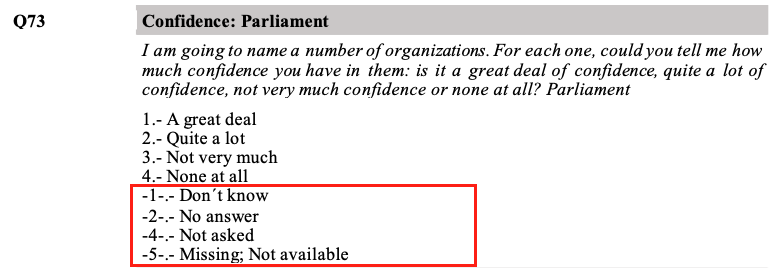
\includegraphics[width=0.7\linewidth]{images/w7_wvs_recode} \end{center}

\begin{center}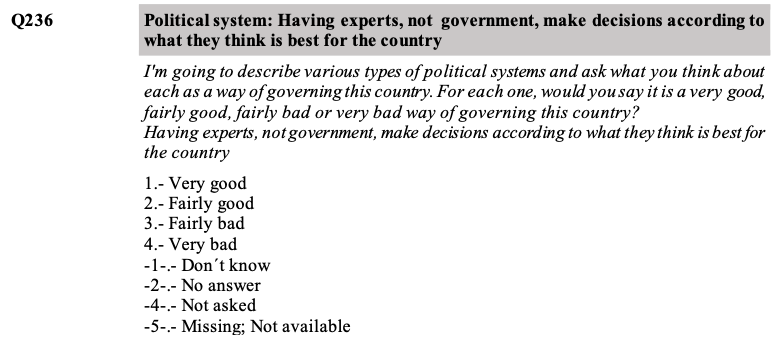
\includegraphics[width=0.7\linewidth]{images/w7_wvs_q236} \end{center}

\begin{Shaded}
\begin{Highlighting}[]
\NormalTok{df\_recode }\OtherTok{\textless{}{-}}\NormalTok{ df }\SpecialCharTok{|\textgreater{}}
  \FunctionTok{mutate}\NormalTok{(}\AttributeTok{Q73=}\FunctionTok{if\_else}\NormalTok{(Q73}\SpecialCharTok{\textless{}}\DecValTok{0}\NormalTok{,}
                    \ConstantTok{NA}\NormalTok{,}
\NormalTok{                    Q73),}
         \AttributeTok{Q236=}\FunctionTok{if\_else}\NormalTok{(Q236}\SpecialCharTok{\textless{}}\DecValTok{0}\NormalTok{,}
                     \ConstantTok{NA}\NormalTok{,}
\NormalTok{                     Q236)) }\SpecialCharTok{|\textgreater{}}
  \FunctionTok{na.omit}\NormalTok{() }\CommentTok{\# drops all rows with NA values}
\end{Highlighting}
\end{Shaded}

\subsubsection*{Examine the variables}\label{examine-the-variables}
\addcontentsline{toc}{subsubsection}{Examine the variables}

Examine the variables to make sure they are as you expect them to be after the transformation.

\begin{Shaded}
\begin{Highlighting}[]
\FunctionTok{summary}\NormalTok{(df\_recode)}
\end{Highlighting}
\end{Shaded}

\begin{verbatim}
##  B_COUNTRY_ALPHA         Q73             Q236      
##  Length:4018        Min.   :1.000   Min.   :1.000  
##  Class :character   1st Qu.:2.000   1st Qu.:2.000  
##  Mode  :character   Median :3.000   Median :2.000  
##                     Mean   :2.602   Mean   :2.487  
##                     3rd Qu.:3.000   3rd Qu.:3.000  
##                     Max.   :4.000   Max.   :4.000
\end{verbatim}

\begin{Shaded}
\begin{Highlighting}[]
\NormalTok{df\_recode }\SpecialCharTok{|\textgreater{}}
  \FunctionTok{ggplot}\NormalTok{(}\FunctionTok{aes}\NormalTok{(}\AttributeTok{x=}\FunctionTok{factor}\NormalTok{(Q73))) }\SpecialCharTok{+}
  \FunctionTok{geom\_bar}\NormalTok{()}
\end{Highlighting}
\end{Shaded}

\pandocbounded{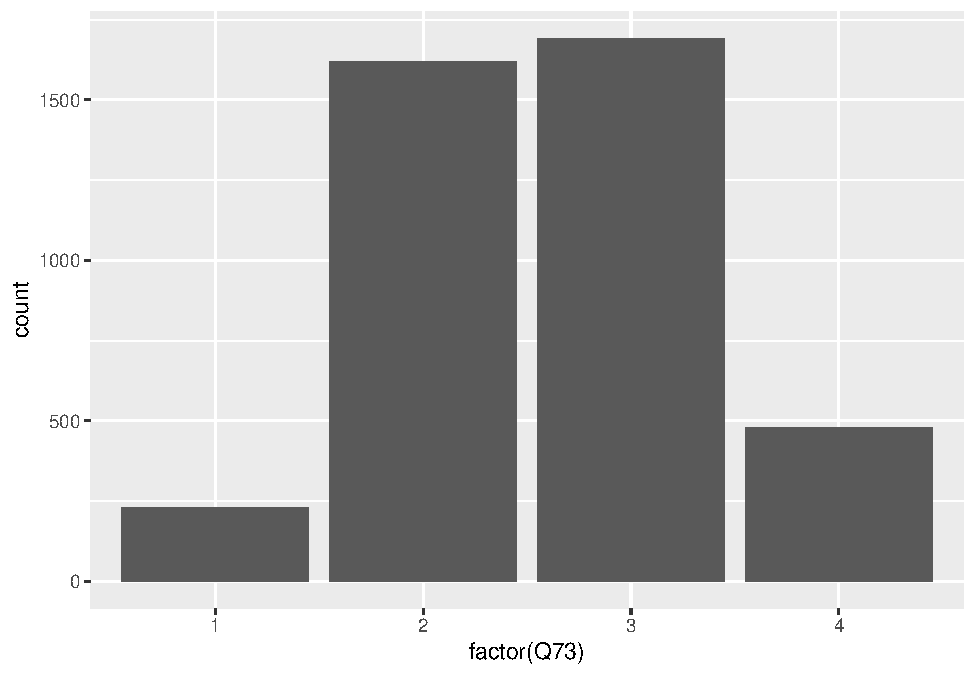
\includegraphics[keepaspectratio]{POL342-tutorial-notes_files/figure-latex/unnamed-chunk-195-1.pdf}}

\begin{Shaded}
\begin{Highlighting}[]
\NormalTok{df\_recode }\SpecialCharTok{|\textgreater{}}
  \FunctionTok{ggplot}\NormalTok{(}\FunctionTok{aes}\NormalTok{(}\AttributeTok{x=}\FunctionTok{factor}\NormalTok{(Q236))) }\SpecialCharTok{+}
  \FunctionTok{geom\_bar}\NormalTok{()}
\end{Highlighting}
\end{Shaded}

\pandocbounded{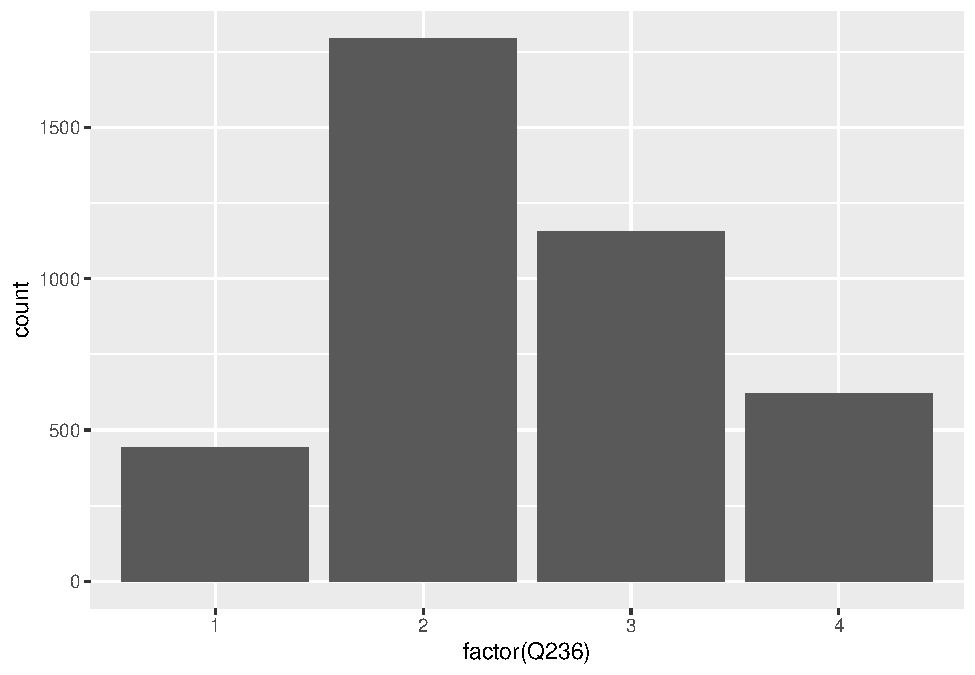
\includegraphics[keepaspectratio]{POL342-tutorial-notes_files/figure-latex/unnamed-chunk-196-1.pdf}}

\begin{Shaded}
\begin{Highlighting}[]
\FunctionTok{tab\_xtab}\NormalTok{(}\AttributeTok{var.col=}\NormalTok{df}\SpecialCharTok{$}\NormalTok{Q73, }\AttributeTok{var.row=}\NormalTok{df}\SpecialCharTok{$}\NormalTok{Q236,}
         \AttributeTok{show.col.prc =} \ConstantTok{TRUE}\NormalTok{)}
\end{Highlighting}
\end{Shaded}

Political system:Having experts, notgovernment, makedecisions accordingto wh

Confidence:Parliament

Total

A great deal

Quite a lot

Not very much

None at all

Very good

{42}{18.3~\%}

{164}{10.1~\%}

{171}{10.1~\%}

{67}{14~\%}

{444}{11.1~\%}

Fairly good

{85}{37~\%}

{700}{43.2~\%}

{829}{49~\%}

{180}{37.7~\%}

{1794}{44.6~\%}

Fairly bad

{62}{27~\%}

{493}{30.5~\%}

{470}{27.8~\%}

{133}{27.8~\%}

{1158}{28.8~\%}

Very bad

{41}{17.8~\%}

{262}{16.2~\%}

{221}{13.1~\%}

{98}{20.5~\%}

{622}{15.5~\%}

Total

{230}{100~\%}

{1619}{100~\%}

{1691}{100~\%}

{478}{100~\%}

{4018}{100~\%}

χ2=51.496 · df=9 · Cramer's V=0.065 · p=0.000

\begin{Shaded}
\begin{Highlighting}[]
\NormalTok{df\_recode }\SpecialCharTok{|\textgreater{}}
  \FunctionTok{ggplot}\NormalTok{(}\FunctionTok{aes}\NormalTok{(}\AttributeTok{x=}\FunctionTok{factor}\NormalTok{(Q73),}\AttributeTok{fill=}\FunctionTok{factor}\NormalTok{(Q236))) }\SpecialCharTok{+}
  \FunctionTok{geom\_bar}\NormalTok{(}\AttributeTok{position=}\StringTok{"fill"}\NormalTok{) }\SpecialCharTok{+}
  \FunctionTok{theme\_bw}\NormalTok{()}
\end{Highlighting}
\end{Shaded}

\pandocbounded{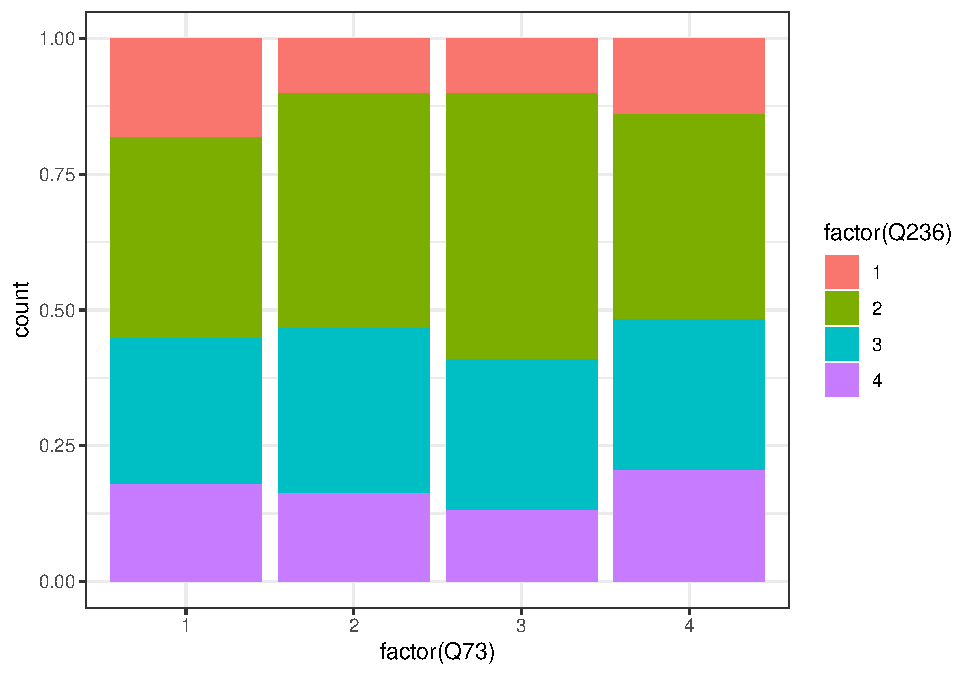
\includegraphics[keepaspectratio]{POL342-tutorial-notes_files/figure-latex/unnamed-chunk-198-1.pdf}}

\begin{Shaded}
\begin{Highlighting}[]
\NormalTok{df\_recode }\SpecialCharTok{|\textgreater{}}
  \FunctionTok{ggplot}\NormalTok{(}\FunctionTok{aes}\NormalTok{(}\AttributeTok{x=}\FunctionTok{factor}\NormalTok{(Q73),}\AttributeTok{fill=}\FunctionTok{factor}\NormalTok{(Q236))) }\SpecialCharTok{+}
  \FunctionTok{geom\_bar}\NormalTok{(}\AttributeTok{position=}\StringTok{"fill"}\NormalTok{) }\SpecialCharTok{+}
  \FunctionTok{theme\_bw}\NormalTok{() }\SpecialCharTok{+}
  \FunctionTok{xlab}\NormalTok{(}\StringTok{"Lack of Confidence in Parliament"}\NormalTok{) }\SpecialCharTok{+}
  \FunctionTok{ylab}\NormalTok{(}\StringTok{"Proportion"}\NormalTok{) }\SpecialCharTok{+}
  \FunctionTok{scale\_fill\_manual}\NormalTok{(}\AttributeTok{name=}\StringTok{"Expert versus Govt"}\NormalTok{, }\CommentTok{\#legend label}
                    \AttributeTok{values =} \FunctionTok{c}\NormalTok{(}\StringTok{"navyblue"}\NormalTok{,}\StringTok{"blue"}\NormalTok{,}\StringTok{"skyblue"}\NormalTok{,}\StringTok{"grey"}\NormalTok{), }\CommentTok{\#color specification}
                    \AttributeTok{labels =} \FunctionTok{c}\NormalTok{(}\StringTok{"Very Good"}\NormalTok{,}\StringTok{"Fairly Good"}\NormalTok{, }\StringTok{"Fairly Bad"}\NormalTok{, }\StringTok{"Very Bad"}\NormalTok{))}
\end{Highlighting}
\end{Shaded}

\pandocbounded{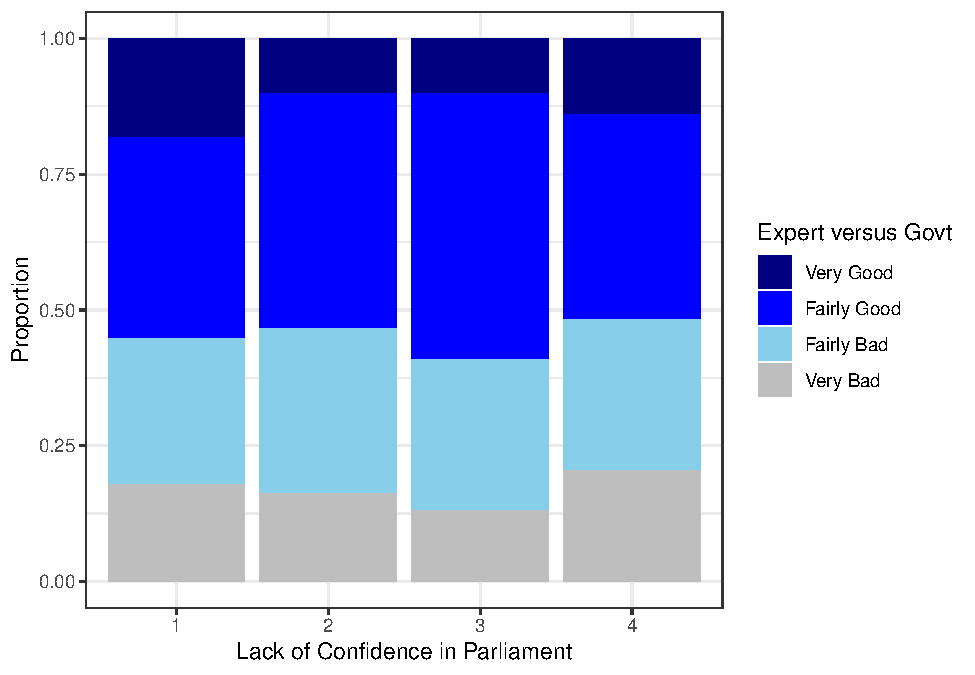
\includegraphics[keepaspectratio]{POL342-tutorial-notes_files/figure-latex/unnamed-chunk-199-1.pdf}}

\subsection*{Other countries}\label{other-countries}
\addcontentsline{toc}{subsection}{Other countries}

\subsubsection*{United States}\label{united-states}
\addcontentsline{toc}{subsubsection}{United States}

\begin{Shaded}
\begin{Highlighting}[]
\FunctionTok{read\_rds}\NormalTok{(}\StringTok{"Project/WVS/WVS\_Cross{-}National\_Wave\_7\_rds\_v6\_0.rds"}\NormalTok{) }\SpecialCharTok{|\textgreater{}}
  \FunctionTok{select}\NormalTok{(vars) }\SpecialCharTok{|\textgreater{}}
  \FunctionTok{filter}\NormalTok{(B\_COUNTRY\_ALPHA}\SpecialCharTok{==}\StringTok{"USA"}\NormalTok{) }\SpecialCharTok{|\textgreater{}}
  \FunctionTok{mutate}\NormalTok{(}\AttributeTok{Q73=}\FunctionTok{if\_else}\NormalTok{(Q73}\SpecialCharTok{\textless{}}\DecValTok{0}\NormalTok{,}
                    \ConstantTok{NA}\NormalTok{,}
\NormalTok{                    Q73),}
         \AttributeTok{Q236=}\FunctionTok{if\_else}\NormalTok{(Q236}\SpecialCharTok{\textless{}}\DecValTok{0}\NormalTok{,}
                     \ConstantTok{NA}\NormalTok{,}
\NormalTok{                     Q236)) }\SpecialCharTok{|\textgreater{}}
  \FunctionTok{na.omit}\NormalTok{() }\SpecialCharTok{|\textgreater{}}
  \FunctionTok{ggplot}\NormalTok{(}\FunctionTok{aes}\NormalTok{(}\AttributeTok{x=}\FunctionTok{factor}\NormalTok{(Q73),}\AttributeTok{fill=}\FunctionTok{factor}\NormalTok{(Q236))) }\SpecialCharTok{+}
  \FunctionTok{geom\_bar}\NormalTok{(}\AttributeTok{position=}\StringTok{"fill"}\NormalTok{) }\SpecialCharTok{+}
  \FunctionTok{theme\_bw}\NormalTok{() }\SpecialCharTok{+}
  \FunctionTok{xlab}\NormalTok{(}\StringTok{"Lack of Confidence in Parliament"}\NormalTok{) }\SpecialCharTok{+}
  \FunctionTok{ylab}\NormalTok{(}\StringTok{"Proportion"}\NormalTok{) }\SpecialCharTok{+}
  \FunctionTok{scale\_fill\_manual}\NormalTok{(}\AttributeTok{name=}\StringTok{"Expert versus Govt"}\NormalTok{, }\CommentTok{\#legend label}
                    \AttributeTok{values =} \FunctionTok{c}\NormalTok{(}\StringTok{"navyblue"}\NormalTok{,}\StringTok{"blue"}\NormalTok{,}\StringTok{"skyblue"}\NormalTok{,}\StringTok{"grey"}\NormalTok{), }\CommentTok{\#color specification}
                    \AttributeTok{labels =} \FunctionTok{c}\NormalTok{(}\StringTok{"Very Good"}\NormalTok{,}\StringTok{"Fairly Good"}\NormalTok{, }\StringTok{"Fairly Bad"}\NormalTok{, }\StringTok{"Very Bad"}\NormalTok{))}
\end{Highlighting}
\end{Shaded}

\pandocbounded{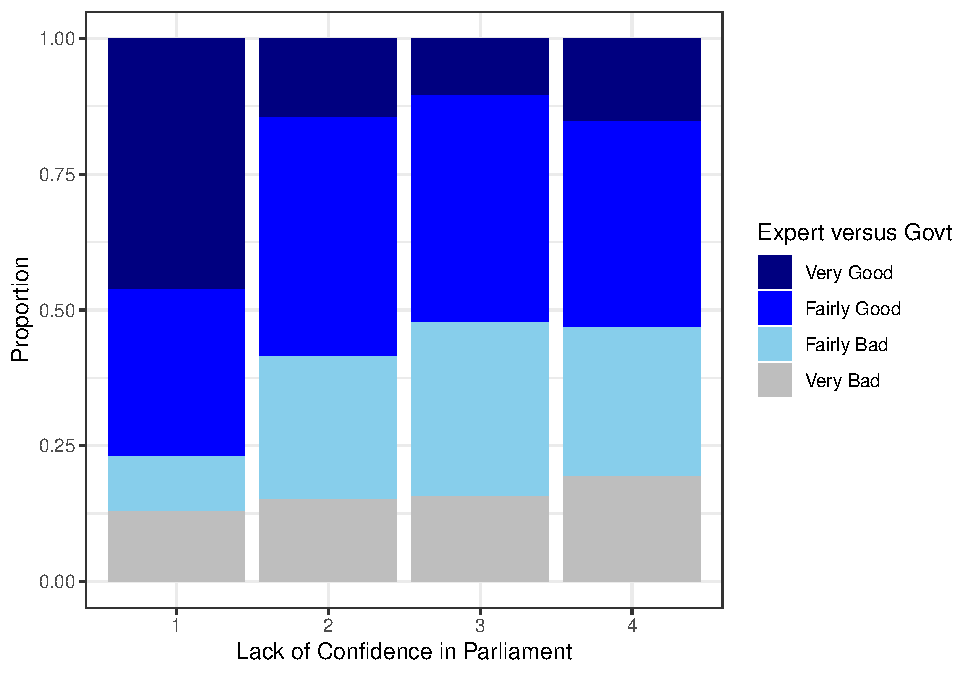
\includegraphics[keepaspectratio]{POL342-tutorial-notes_files/figure-latex/unnamed-chunk-200-1.pdf}}

\subsubsection*{Japan}\label{japan}
\addcontentsline{toc}{subsubsection}{Japan}

\begin{Shaded}
\begin{Highlighting}[]
\FunctionTok{read\_rds}\NormalTok{(}\StringTok{"Project/WVS/WVS\_Cross{-}National\_Wave\_7\_rds\_v6\_0.rds"}\NormalTok{) }\SpecialCharTok{|\textgreater{}}
  \FunctionTok{select}\NormalTok{(vars) }\SpecialCharTok{|\textgreater{}}
  \FunctionTok{filter}\NormalTok{(B\_COUNTRY\_ALPHA}\SpecialCharTok{==}\StringTok{"JPN"}\NormalTok{) }\SpecialCharTok{|\textgreater{}}
  \FunctionTok{mutate}\NormalTok{(}\AttributeTok{Q73=}\FunctionTok{if\_else}\NormalTok{(Q73}\SpecialCharTok{\textless{}}\DecValTok{0}\NormalTok{,}
                    \ConstantTok{NA}\NormalTok{,}
\NormalTok{                    Q73),}
         \AttributeTok{Q236=}\FunctionTok{if\_else}\NormalTok{(Q236}\SpecialCharTok{\textless{}}\DecValTok{0}\NormalTok{,}
                     \ConstantTok{NA}\NormalTok{,}
\NormalTok{                     Q236)) }\SpecialCharTok{|\textgreater{}}
  \FunctionTok{na.omit}\NormalTok{() }\SpecialCharTok{|\textgreater{}}
  \FunctionTok{ggplot}\NormalTok{(}\FunctionTok{aes}\NormalTok{(}\AttributeTok{x=}\FunctionTok{factor}\NormalTok{(Q73),}\AttributeTok{fill=}\FunctionTok{factor}\NormalTok{(Q236))) }\SpecialCharTok{+}
  \FunctionTok{geom\_bar}\NormalTok{(}\AttributeTok{position=}\StringTok{"fill"}\NormalTok{) }\SpecialCharTok{+}
  \FunctionTok{theme\_bw}\NormalTok{() }\SpecialCharTok{+}
  \FunctionTok{xlab}\NormalTok{(}\StringTok{"Lack of Confidence in Parliament"}\NormalTok{) }\SpecialCharTok{+}
  \FunctionTok{ylab}\NormalTok{(}\StringTok{"Proportion"}\NormalTok{) }\SpecialCharTok{+}
  \FunctionTok{scale\_fill\_manual}\NormalTok{(}\AttributeTok{name=}\StringTok{"Expert versus Govt"}\NormalTok{, }\CommentTok{\#legend label}
                    \AttributeTok{values =} \FunctionTok{c}\NormalTok{(}\StringTok{"navyblue"}\NormalTok{,}\StringTok{"blue"}\NormalTok{,}\StringTok{"skyblue"}\NormalTok{,}\StringTok{"grey"}\NormalTok{), }\CommentTok{\#color specification}
                    \AttributeTok{labels =} \FunctionTok{c}\NormalTok{(}\StringTok{"Very Good"}\NormalTok{,}\StringTok{"Fairly Good"}\NormalTok{, }\StringTok{"Fairly Bad"}\NormalTok{, }\StringTok{"Very Bad"}\NormalTok{))}
\end{Highlighting}
\end{Shaded}

\pandocbounded{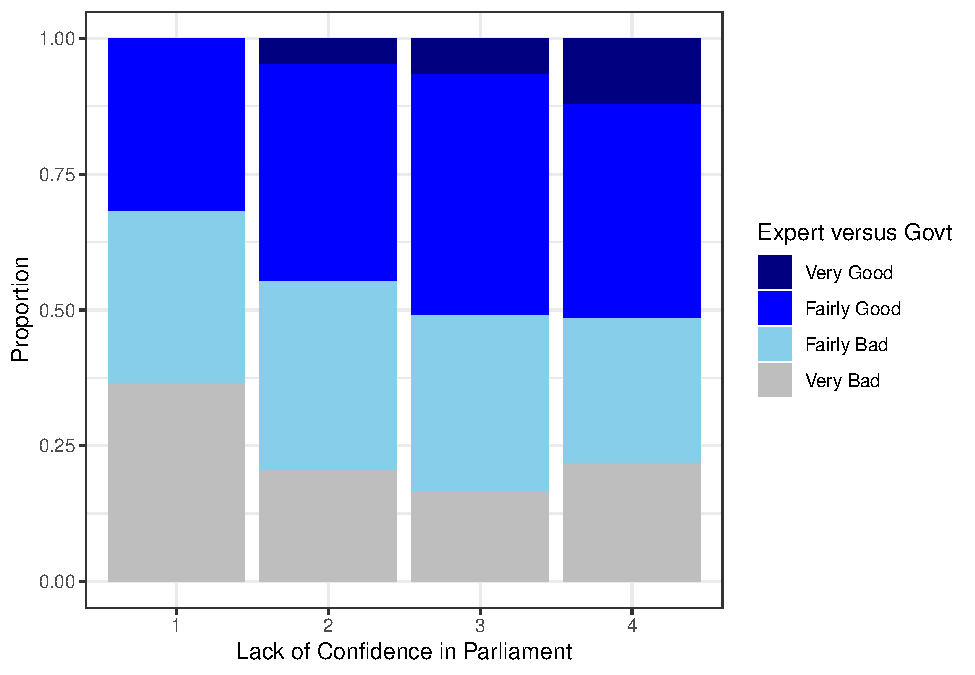
\includegraphics[keepaspectratio]{POL342-tutorial-notes_files/figure-latex/unnamed-chunk-201-1.pdf}}

\subsection*{Remove all from environment}\label{remove-all-from-environment-1}
\addcontentsline{toc}{subsection}{Remove all from environment}

To avoid any misspecification of variables, clear environment before moving on to the next dataset.

\begin{Shaded}
\begin{Highlighting}[]
\FunctionTok{rm}\NormalTok{(}\AttributeTok{list=}\FunctionTok{ls}\NormalTok{())}
\end{Highlighting}
\end{Shaded}

\section{Asian Barometer (Wave 5, 2018-2021)}\label{asian-barometer-wave-5-2018-2021}

\subsection*{Step 2: Select your variables}\label{step-2-select-your-variables-3}
\addcontentsline{toc}{subsection}{Step 2: Select your variables}

Look at the codebook and choose your variables. I have chosen the following

\begin{Shaded}
\begin{Highlighting}[]
\NormalTok{Independent variable}\SpecialCharTok{:}\NormalTok{ Views toward the US}
\DecValTok{175}\NormalTok{ Does the United States do more good or harm to Asia?}
\DecValTok{184}\SpecialCharTok{:}\NormalTok{ General speaking, the influence the United States has on our country is?}

\NormalTok{DV}\SpecialCharTok{:}\NormalTok{ Views toward }\FunctionTok{democracy}\NormalTok{ (}\DecValTok{1}\NormalTok{ strongly agree }\SpecialCharTok{{-}} \DecValTok{4}\NormalTok{ strongly disagree)}
\DecValTok{169}\NormalTok{ Democratic regimes are indecisive and full of problems}
\end{Highlighting}
\end{Shaded}

\begin{Shaded}
\begin{Highlighting}[]
\NormalTok{vars }\OtherTok{\textless{}{-}} \FunctionTok{c}\NormalTok{(}\StringTok{"country"}\NormalTok{,}\StringTok{"Year"}\NormalTok{,}
           \StringTok{"q175"}\NormalTok{,}\StringTok{"q184"}\NormalTok{,}
           \StringTok{"q169"}\NormalTok{)}
\end{Highlighting}
\end{Shaded}

\subsection*{Step 3: Trim down your data set}\label{step-3-trim-down-your-data-set-1}
\addcontentsline{toc}{subsection}{Step 3: Trim down your data set}

\subsubsection*{For the Asian Barometer data set, select one country}\label{for-the-asian-barometer-data-set-select-one-country}
\addcontentsline{toc}{subsubsection}{For the Asian Barometer data set, select one country}

\begin{Shaded}
\begin{Highlighting}[]
\NormalTok{df }\OtherTok{\textless{}{-}} \FunctionTok{read\_dta}\NormalTok{(}\StringTok{"Project/asianbarometer\_wave5/20230504\_W5\_merge\_15.dta"}\NormalTok{) }\SpecialCharTok{|\textgreater{}}
  \FunctionTok{select}\NormalTok{(vars) }\SpecialCharTok{|\textgreater{}}
  \FunctionTok{filter}\NormalTok{(country}\SpecialCharTok{==}\DecValTok{3}\NormalTok{) }\CommentTok{\# South Korea (refer to codebook)}

\FunctionTok{summary}\NormalTok{(df)}
\end{Highlighting}
\end{Shaded}

\begin{verbatim}
##     country       Year           q175            q184            q169     
##  Min.   :3   Min.   :2019   Min.   :1.000   Min.   :1.000   Min.   :1.00  
##  1st Qu.:3   1st Qu.:2019   1st Qu.:2.000   1st Qu.:2.000   1st Qu.:3.00  
##  Median :3   Median :2019   Median :2.000   Median :3.000   Median :3.00  
##  Mean   :3   Mean   :2019   Mean   :2.797   Mean   :3.068   Mean   :3.14  
##  3rd Qu.:3   3rd Qu.:2019   3rd Qu.:3.000   3rd Qu.:3.000   3rd Qu.:4.00  
##  Max.   :3   Max.   :2019   Max.   :9.000   Max.   :9.000   Max.   :9.00
\end{verbatim}

\subsubsection*{\texorpdfstring{Replace nominal categories not found on the ordinal scale to \texttt{NA}}{Replace nominal categories not found on the ordinal scale to NA}}\label{replace-nominal-categories-not-found-on-the-ordinal-scale-to-na-1}
\addcontentsline{toc}{subsubsection}{Replace nominal categories not found on the ordinal scale to \texttt{NA}}

\begin{Shaded}
\begin{Highlighting}[]
\NormalTok{df\_recode }\OtherTok{\textless{}{-}}\NormalTok{ df }\SpecialCharTok{|\textgreater{}}
  \FunctionTok{mutate}\NormalTok{(}\AttributeTok{q169 =} \FunctionTok{if\_else}\NormalTok{(q169 }\SpecialCharTok{\textgreater{}} \DecValTok{4}\NormalTok{, }\ConstantTok{NA}\NormalTok{, q169),}
         \AttributeTok{q175 =} \FunctionTok{if\_else}\NormalTok{(q175 }\SpecialCharTok{\textgreater{}} \DecValTok{4}\NormalTok{, }\ConstantTok{NA}\NormalTok{, q175),}
         \AttributeTok{q184 =} \FunctionTok{if\_else}\NormalTok{(q184 }\SpecialCharTok{\textgreater{}} \DecValTok{4}\NormalTok{, }\ConstantTok{NA}\NormalTok{, q184)) }\SpecialCharTok{|\textgreater{}}
  \FunctionTok{na.omit}\NormalTok{()}
\end{Highlighting}
\end{Shaded}

\subsection*{Step 4: Examine the univariate distribution and bivariate relationship}\label{step-4-examine-the-univariate-distribution-and-bivariate-relationship-3}
\addcontentsline{toc}{subsection}{Step 4: Examine the univariate distribution and bivariate relationship}

\begin{Shaded}
\begin{Highlighting}[]
\NormalTok{df\_recode }\SpecialCharTok{|\textgreater{}}
  \FunctionTok{ggplot}\NormalTok{(}\FunctionTok{aes}\NormalTok{(}\AttributeTok{x=}\FunctionTok{factor}\NormalTok{(q169))) }\SpecialCharTok{+}
  \FunctionTok{geom\_bar}\NormalTok{()}
\end{Highlighting}
\end{Shaded}

\pandocbounded{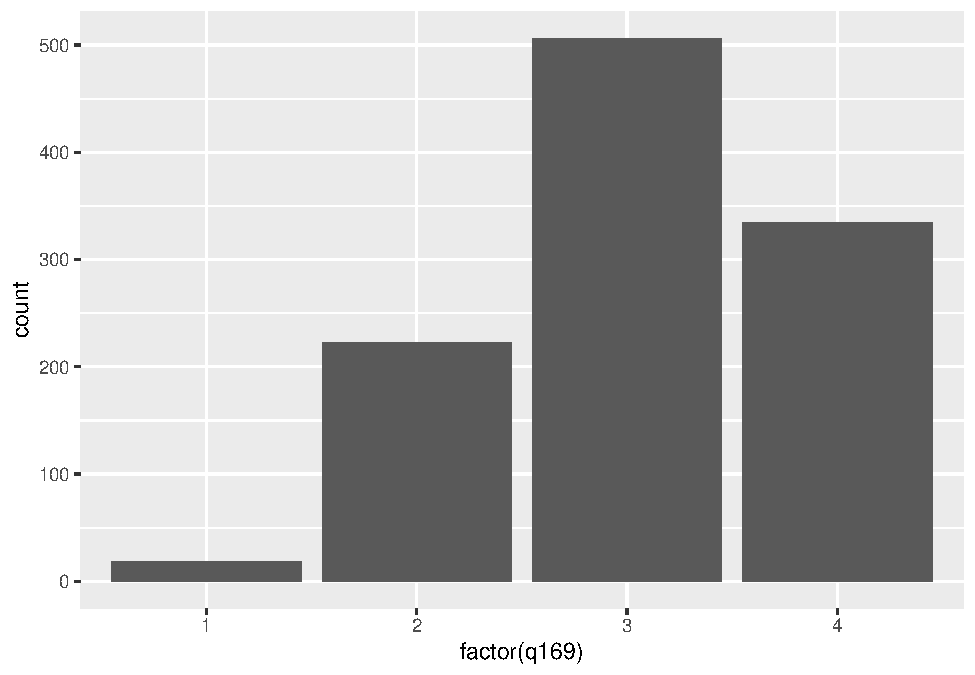
\includegraphics[keepaspectratio]{POL342-tutorial-notes_files/figure-latex/unnamed-chunk-208-1.pdf}}

\begin{Shaded}
\begin{Highlighting}[]
\NormalTok{df\_recode }\SpecialCharTok{|\textgreater{}}
  \FunctionTok{ggplot}\NormalTok{(}\FunctionTok{aes}\NormalTok{(}\AttributeTok{x=}\FunctionTok{factor}\NormalTok{(q175))) }\SpecialCharTok{+}
  \FunctionTok{geom\_bar}\NormalTok{()}
\end{Highlighting}
\end{Shaded}

\pandocbounded{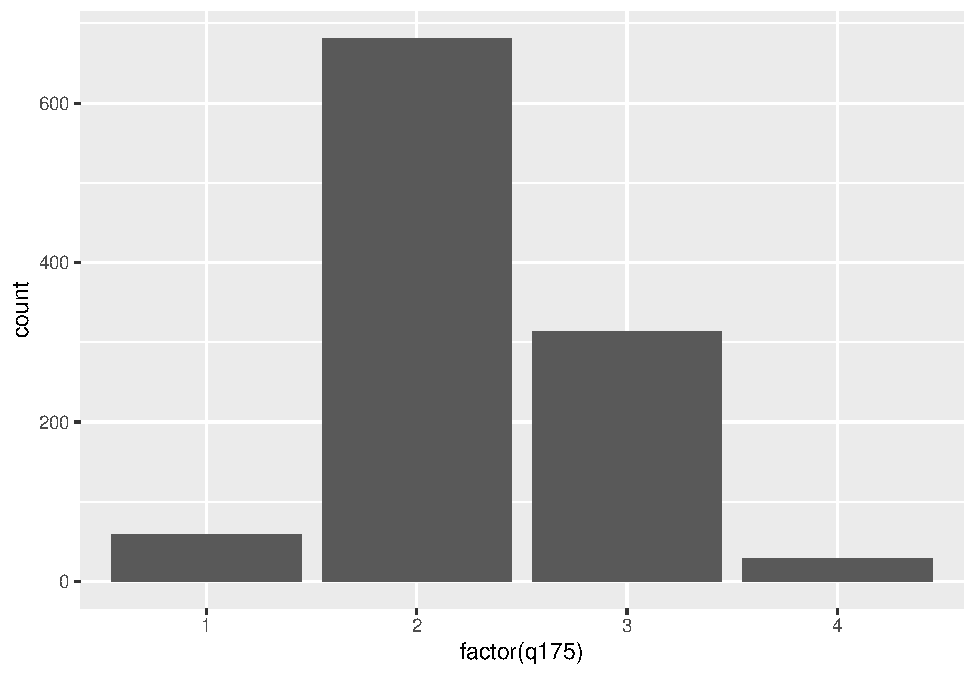
\includegraphics[keepaspectratio]{POL342-tutorial-notes_files/figure-latex/unnamed-chunk-209-1.pdf}}

\subsubsection*{Examining the relationship of perceptions of US and views of democracy}\label{examining-the-relationship-of-perceptions-of-us-and-views-of-democracy}
\addcontentsline{toc}{subsubsection}{Examining the relationship of perceptions of US and views of democracy}

\subsubsection*{DV1: q175}\label{dv1-q175}
\addcontentsline{toc}{subsubsection}{DV1: q175}

\begin{Shaded}
\begin{Highlighting}[]
\NormalTok{df\_recode }\SpecialCharTok{|\textgreater{}}
  \FunctionTok{ggplot}\NormalTok{(}\FunctionTok{aes}\NormalTok{(}\AttributeTok{fill=}\FunctionTok{factor}\NormalTok{(q169),}\AttributeTok{x=}\FunctionTok{factor}\NormalTok{(q175))) }\SpecialCharTok{+}
  \FunctionTok{geom\_bar}\NormalTok{(}\AttributeTok{position=}\StringTok{"fill"}\NormalTok{) }\SpecialCharTok{+}
  \FunctionTok{theme\_bw}\NormalTok{()}
\end{Highlighting}
\end{Shaded}

\pandocbounded{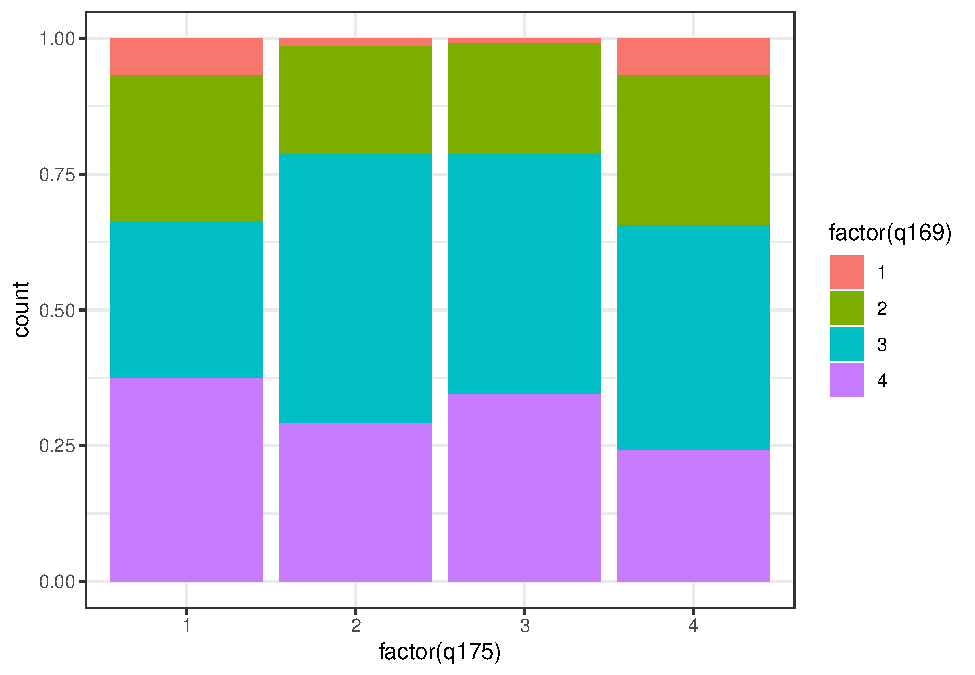
\includegraphics[keepaspectratio]{POL342-tutorial-notes_files/figure-latex/unnamed-chunk-210-1.pdf}}

\subsubsection*{DV2: q184}\label{dv2-q184}
\addcontentsline{toc}{subsubsection}{DV2: q184}

\begin{Shaded}
\begin{Highlighting}[]
\NormalTok{df\_recode }\SpecialCharTok{|\textgreater{}}
  \FunctionTok{ggplot}\NormalTok{(}\FunctionTok{aes}\NormalTok{(}\AttributeTok{fill=}\FunctionTok{factor}\NormalTok{(q169),}\AttributeTok{x=}\FunctionTok{factor}\NormalTok{(q184))) }\SpecialCharTok{+}
  \FunctionTok{geom\_bar}\NormalTok{(}\AttributeTok{position=}\StringTok{"fill"}\NormalTok{) }\SpecialCharTok{+}
  \FunctionTok{theme\_bw}\NormalTok{()}
\end{Highlighting}
\end{Shaded}

\pandocbounded{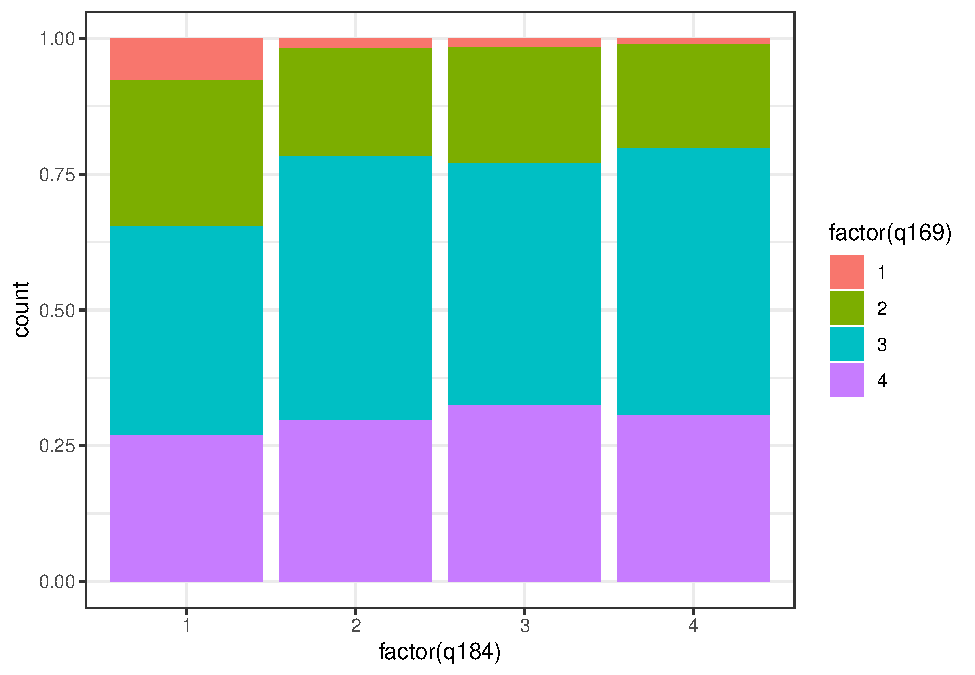
\includegraphics[keepaspectratio]{POL342-tutorial-notes_files/figure-latex/unnamed-chunk-211-1.pdf}}

\section{Canadian Election Study 2021}\label{canadian-election-study-2021}

\subsection*{Step 2: Select your variables}\label{step-2-select-your-variables-4}
\addcontentsline{toc}{subsection}{Step 2: Select your variables}

Look at the codebook and choose your variables.

\begin{Shaded}
\begin{Highlighting}[]
\NormalTok{vars }\OtherTok{\textless{}{-}} \FunctionTok{c}\NormalTok{(}\StringTok{"cps21\_news\_cons"}\NormalTok{,}\StringTok{"cps21\_govt\_confusing"}\NormalTok{) }\CommentTok{\#news consumption and internal political efficacy}
\end{Highlighting}
\end{Shaded}

\subsection*{Step 3: Trim down your data set}\label{step-3-trim-down-your-data-set-2}
\addcontentsline{toc}{subsection}{Step 3: Trim down your data set}

For CES2021, we don't need the \texttt{year} specification.

\begin{Shaded}
\begin{Highlighting}[]
\NormalTok{ces\_select }\OtherTok{\textless{}{-}} \FunctionTok{read\_dta}\NormalTok{(}\StringTok{"Project/CES2021/2021 Canadian Election Study v2.0.dta"}\NormalTok{) }\SpecialCharTok{|\textgreater{}}
  \FunctionTok{select}\NormalTok{(vars)}
\end{Highlighting}
\end{Shaded}

\subsection*{Step 4: Examine the univariate distribution and bivariate relationship}\label{step-4-examine-the-univariate-distribution-and-bivariate-relationship-4}
\addcontentsline{toc}{subsection}{Step 4: Examine the univariate distribution and bivariate relationship}

\subsubsection*{Look at the summary statistics}\label{look-at-the-summary-statistics-1}
\addcontentsline{toc}{subsubsection}{Look at the summary statistics}

Note that the ordinal variables are measured as numerical variables.

\begin{Shaded}
\begin{Highlighting}[]
\FunctionTok{summary}\NormalTok{(ces\_select)}
\end{Highlighting}
\end{Shaded}

\begin{verbatim}
##  cps21_news_cons cps21_govt_confusing
##  Min.   :1.000   Min.   :1.000       
##  1st Qu.:3.000   1st Qu.:2.000       
##  Median :4.000   Median :3.000       
##  Mean   :3.791   Mean   :2.563       
##  3rd Qu.:5.000   3rd Qu.:3.000       
##  Max.   :7.000   Max.   :5.000       
##  NA's   :48
\end{verbatim}

\subsubsection*{Examine the variables}\label{examine-the-variables-1}
\addcontentsline{toc}{subsubsection}{Examine the variables}

Bar chart for ordinal variables. Remember to change the numerical variable into

\begin{Shaded}
\begin{Highlighting}[]
\FunctionTok{ggplot}\NormalTok{(ces\_select,}\FunctionTok{aes}\NormalTok{(}\AttributeTok{x=}\FunctionTok{factor}\NormalTok{(cps21\_news\_cons))) }\SpecialCharTok{+}
  \FunctionTok{geom\_bar}\NormalTok{()}
\end{Highlighting}
\end{Shaded}

\pandocbounded{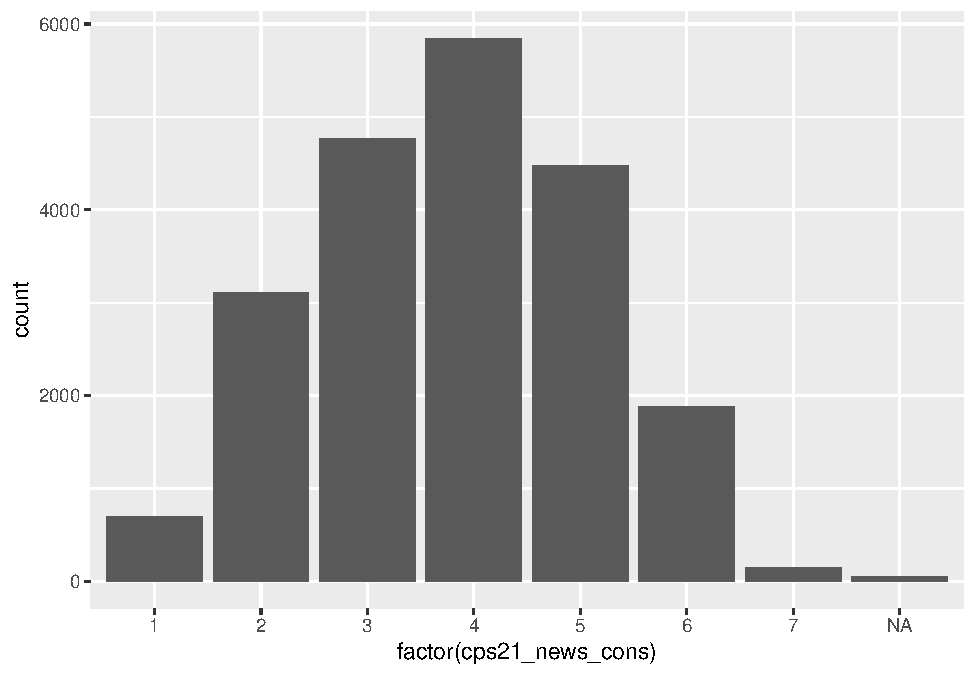
\includegraphics[keepaspectratio]{POL342-tutorial-notes_files/figure-latex/unnamed-chunk-215-1.pdf}}

\begin{Shaded}
\begin{Highlighting}[]
\FunctionTok{ggplot}\NormalTok{(ces\_select,}\FunctionTok{aes}\NormalTok{(}\AttributeTok{x=}\FunctionTok{factor}\NormalTok{(cps21\_govt\_confusing))) }\SpecialCharTok{+}
  \FunctionTok{geom\_bar}\NormalTok{()}
\end{Highlighting}
\end{Shaded}

\pandocbounded{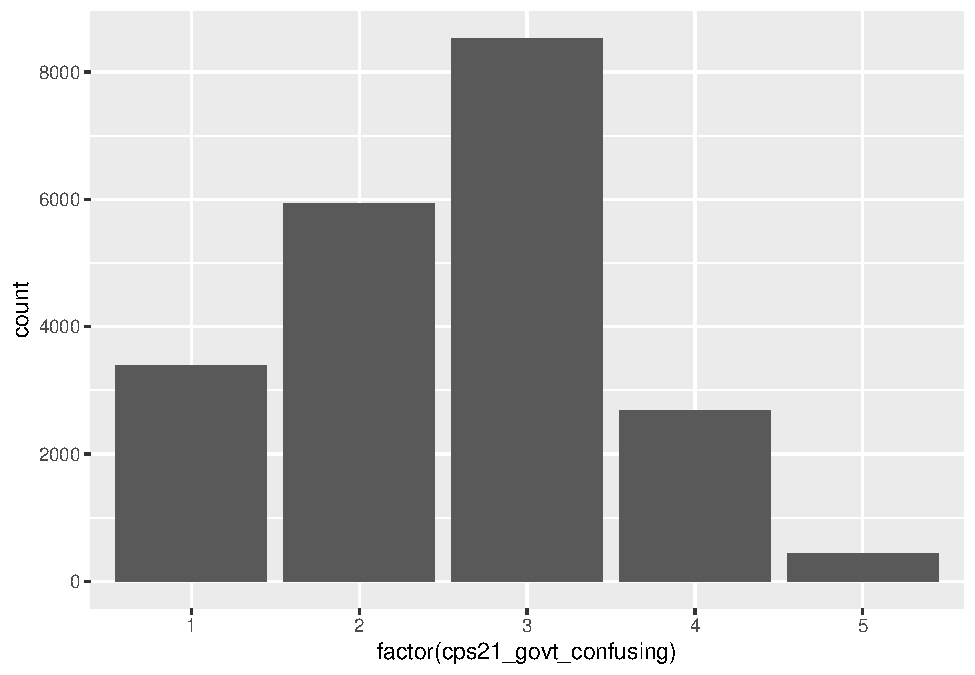
\includegraphics[keepaspectratio]{POL342-tutorial-notes_files/figure-latex/unnamed-chunk-216-1.pdf}}

\subsubsection*{\texorpdfstring{Replace nominal categories not found on the ordinal scale to \texttt{NA}}{Replace nominal categories not found on the ordinal scale to NA}}\label{replace-nominal-categories-not-found-on-the-ordinal-scale-to-na-2}
\addcontentsline{toc}{subsubsection}{Replace nominal categories not found on the ordinal scale to \texttt{NA}}

\begin{center}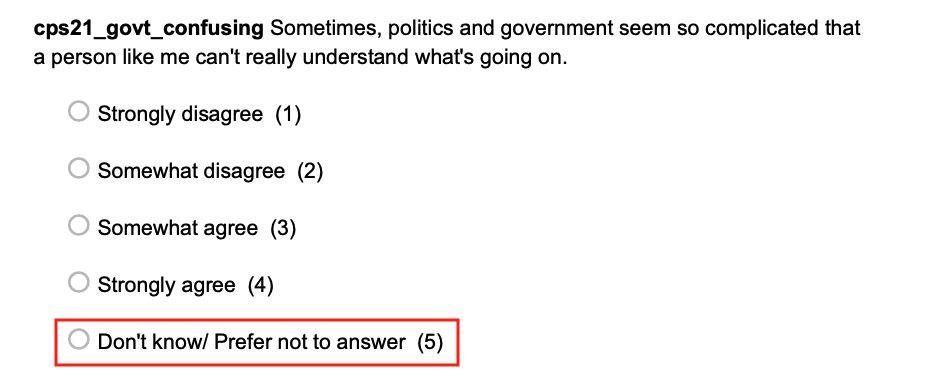
\includegraphics[width=0.7\linewidth]{images/w7_cps_confusing} \end{center}

Use \texttt{if\_else()} function to manipulate variable

\begin{Shaded}
\begin{Highlighting}[]
\NormalTok{ces\_dropna }\OtherTok{\textless{}{-}}\NormalTok{ ces\_select }\SpecialCharTok{|\textgreater{}}
  \FunctionTok{mutate}\NormalTok{(}\AttributeTok{cps21\_govt\_confusing=}\FunctionTok{if\_else}\NormalTok{(cps21\_govt\_confusing}\SpecialCharTok{==}\DecValTok{5}\NormalTok{, }\CommentTok{\#conditional statement}
                                     \ConstantTok{NA}\NormalTok{, }\CommentTok{\#if yes}
\NormalTok{                                     cps21\_govt\_confusing), }\CommentTok{\#if no}
         \AttributeTok{cps21\_news\_cons=}\FunctionTok{if\_else}\NormalTok{(cps21\_news\_cons}\SpecialCharTok{==}\DecValTok{7}\NormalTok{, }\CommentTok{\#conditional statement}
                                \ConstantTok{NA}\NormalTok{, }\CommentTok{\#if yes}
\NormalTok{                                cps21\_news\_cons)) }\SpecialCharTok{|\textgreater{}} \CommentTok{\#if no}
  \FunctionTok{na.omit}\NormalTok{() }\CommentTok{\#remove NAs}
\end{Highlighting}
\end{Shaded}

\subsubsection*{Bivariate relationship}\label{bivariate-relationship-1}
\addcontentsline{toc}{subsubsection}{Bivariate relationship}

If both variables nominal/ordinal variable, you can plot the stacked bar chart.

\begin{Shaded}
\begin{Highlighting}[]
\NormalTok{ces\_dropna }\SpecialCharTok{|\textgreater{}}
  \FunctionTok{ggplot}\NormalTok{(}\FunctionTok{aes}\NormalTok{(}\AttributeTok{x=}\FunctionTok{factor}\NormalTok{(cps21\_news\_cons),}\AttributeTok{fill=}\FunctionTok{factor}\NormalTok{(cps21\_govt\_confusing))) }\SpecialCharTok{+}
  \FunctionTok{geom\_bar}\NormalTok{(}\AttributeTok{position=}\StringTok{"fill"}\NormalTok{) }\SpecialCharTok{+}
  \FunctionTok{theme\_bw}\NormalTok{()}
\end{Highlighting}
\end{Shaded}

\pandocbounded{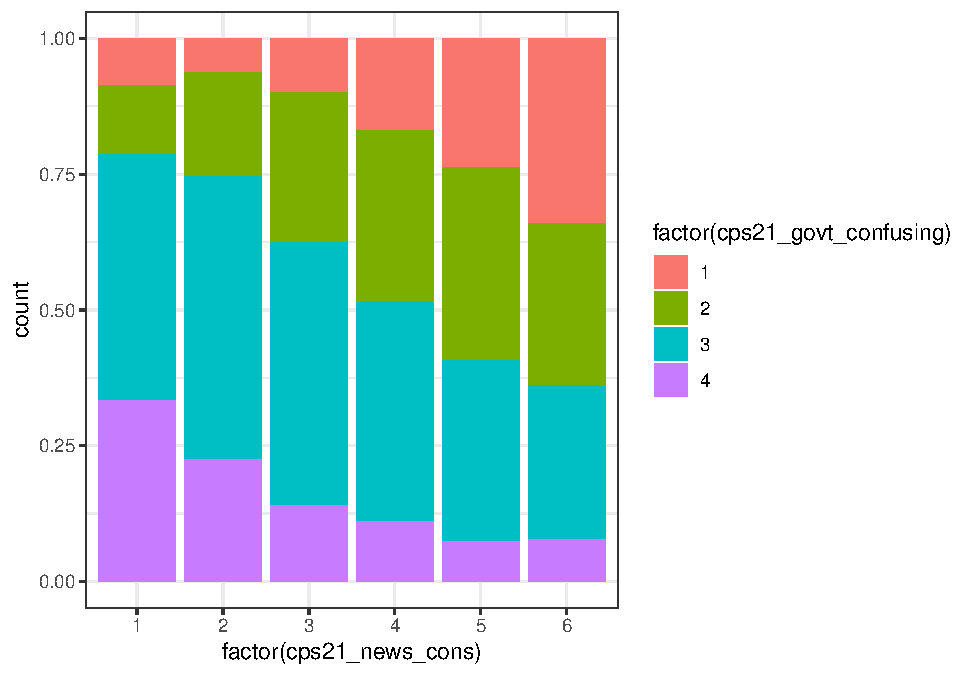
\includegraphics[keepaspectratio]{POL342-tutorial-notes_files/figure-latex/unnamed-chunk-219-1.pdf}}

\subsection*{Remove all from environment}\label{remove-all-from-environment-2}
\addcontentsline{toc}{subsection}{Remove all from environment}

To avoid any misspecification of variables, clear environment before moving on to the next dataset.

\begin{Shaded}
\begin{Highlighting}[]
\FunctionTok{rm}\NormalTok{(}\AttributeTok{list=}\FunctionTok{ls}\NormalTok{())}
\end{Highlighting}
\end{Shaded}

\chapter{Crosstabs using continuous variables}\label{crosstabs-using-continuous-variables}

\begin{itemize}
\tightlist
\item
  Goals for today's class:

  \begin{itemize}
  \tightlist
  \item
    Transforming continuous variables into ordinal variables
  \item
    Creating cross-tabs
  \item
    Saving cross-tabs
  \end{itemize}
\end{itemize}

\section{Set-up}\label{set-up-1}

\subsection*{\texorpdfstring{Make sure you have your project datasets and \texttt{W9.R}}{Make sure you have your project datasets and W9.R}}\label{make-sure-you-have-your-project-datasets-and-w9.r}
\addcontentsline{toc}{subsection}{Make sure you have your project datasets and \texttt{W9.R}}

\begin{center}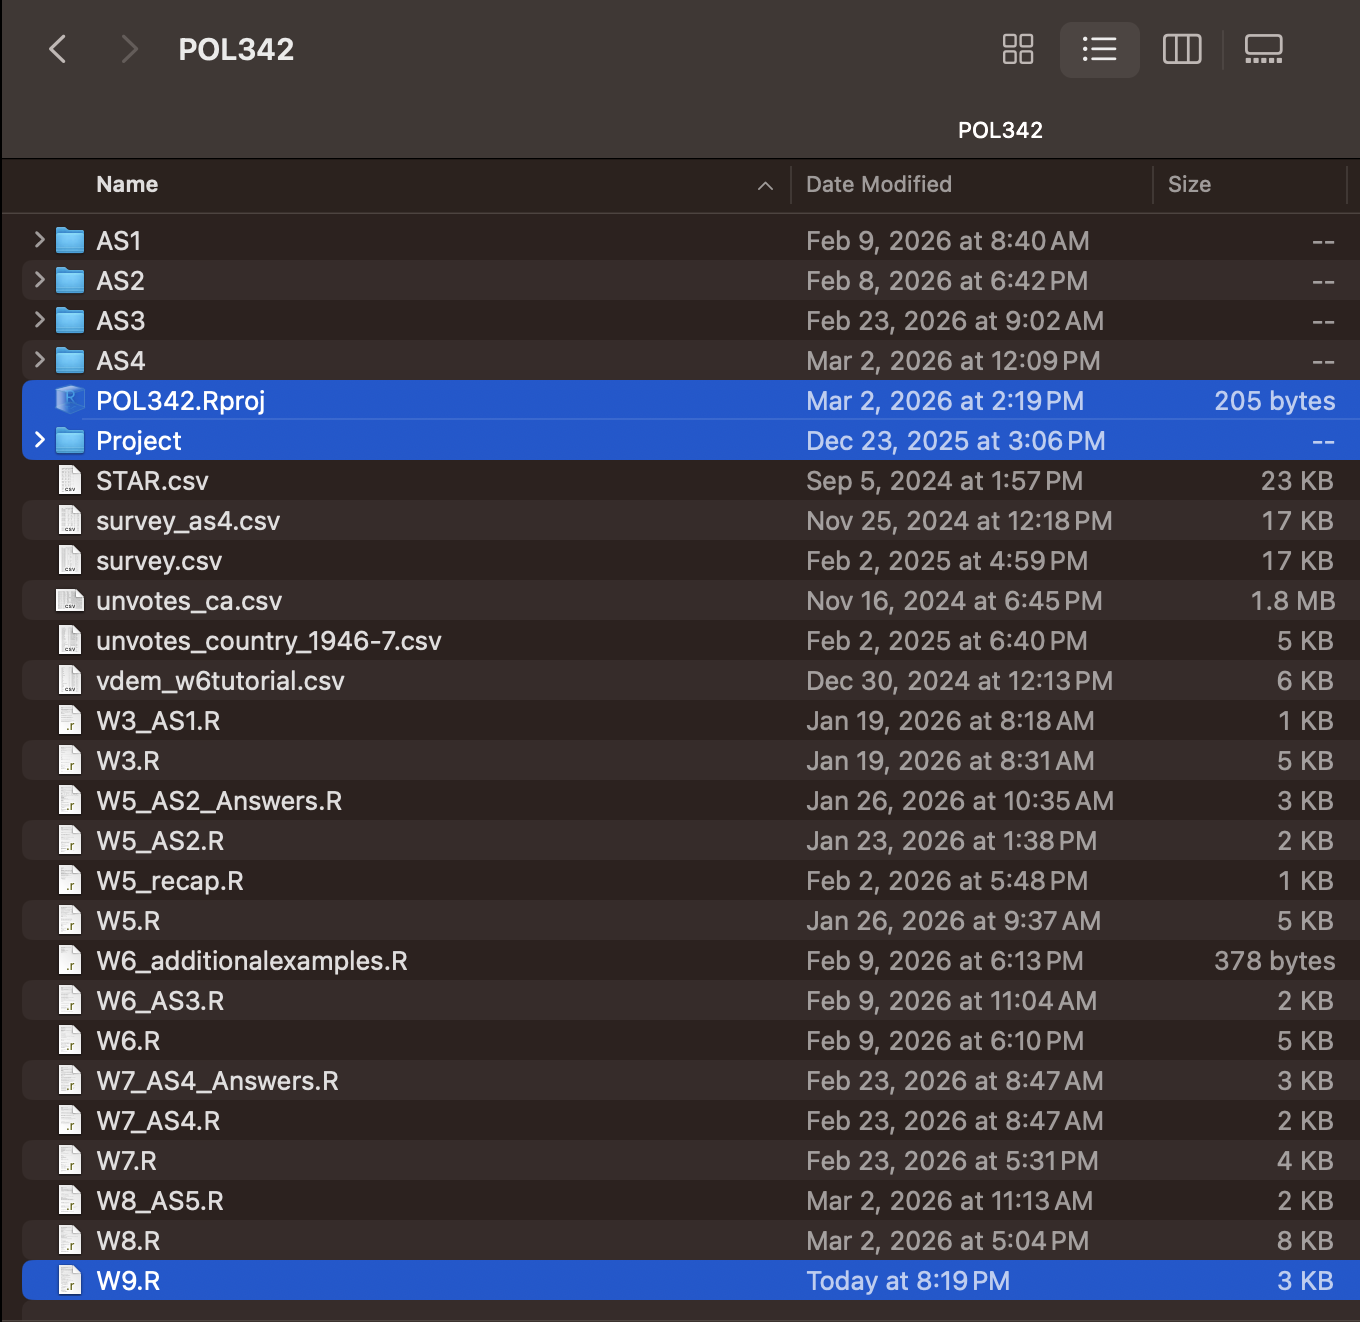
\includegraphics[width=1\linewidth]{images/w8} \end{center}

\subsection*{Load libraries}\label{load-libraries-1}
\addcontentsline{toc}{subsection}{Load libraries}

\begin{Shaded}
\begin{Highlighting}[]
\FunctionTok{library}\NormalTok{(tidyverse)}
\CommentTok{\# install.packages("haven") \# if you haven\textquotesingle{}t installed the package}
\FunctionTok{library}\NormalTok{(haven)}
\FunctionTok{library}\NormalTok{(sjPlot)}
\end{Highlighting}
\end{Shaded}

\section{VDem}\label{vdem-1}

\subsection*{Load Data}\label{load-data-2}
\addcontentsline{toc}{subsection}{Load Data}

\begin{Shaded}
\begin{Highlighting}[]
\NormalTok{vars }\OtherTok{\textless{}{-}} \FunctionTok{c}\NormalTok{(}\StringTok{"country\_name"}\NormalTok{, }\StringTok{"country\_id"}\NormalTok{, }\StringTok{"year"}\NormalTok{, }
          \StringTok{"v2x\_libdem"}\NormalTok{,}\StringTok{"e\_gdppc"}\NormalTok{,}\StringTok{"v2mefemjrn"}\NormalTok{, }\StringTok{"v2pepwrgen"}\NormalTok{)}

\NormalTok{vdem\_selected }\OtherTok{\textless{}{-}} \FunctionTok{read.csv}\NormalTok{(}\StringTok{"Project/VDem/VDem\_post2000.csv"}\NormalTok{) }\SpecialCharTok{|\textgreater{}}
  \FunctionTok{select}\NormalTok{(}\FunctionTok{all\_of}\NormalTok{(vars)) }\SpecialCharTok{|\textgreater{}}
  \FunctionTok{filter}\NormalTok{(year}\SpecialCharTok{==}\DecValTok{2010}\NormalTok{) }
\end{Highlighting}
\end{Shaded}

\begin{itemize}
\tightlist
\item
  Variables selected:

  \begin{itemize}
  \tightlist
  \item
    \texttt{v2x\_libdem}: Liberal democracy index
  \item
    \texttt{e\_gdppc}: GDP per capita
  \item
    \texttt{v2mefemjrn}: \% of female journalist
  \item
    \texttt{v2pepwrgen}: Power distributed by gender
  \end{itemize}
\end{itemize}

\subsection*{\texorpdfstring{Create ordinal categories using function \texttt{cut()}}{Create ordinal categories using function cut()}}\label{create-ordinal-categories-using-function-cut}
\addcontentsline{toc}{subsection}{Create ordinal categories using function \texttt{cut()}}

\begin{Shaded}
\begin{Highlighting}[]
\NormalTok{?cut }\CommentTok{\# pull up the documentation for \textasciigrave{}cut()\textasciigrave{}}
\end{Highlighting}
\end{Shaded}

\begin{center}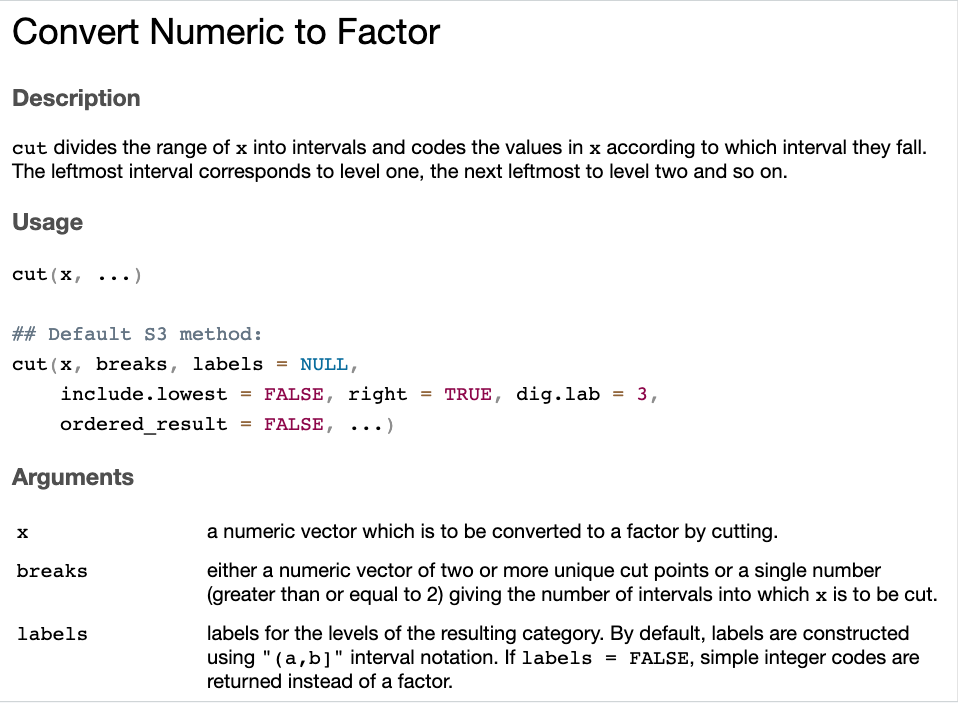
\includegraphics[width=1\linewidth]{images/w8_cut} \end{center}

\subsubsection*{Consider this variable: v2mefemjrn (\% of female journalists)}\label{consider-this-variable-v2mefemjrn-of-female-journalists}
\addcontentsline{toc}{subsubsection}{Consider this variable: v2mefemjrn (\% of female journalists)}

\begin{center}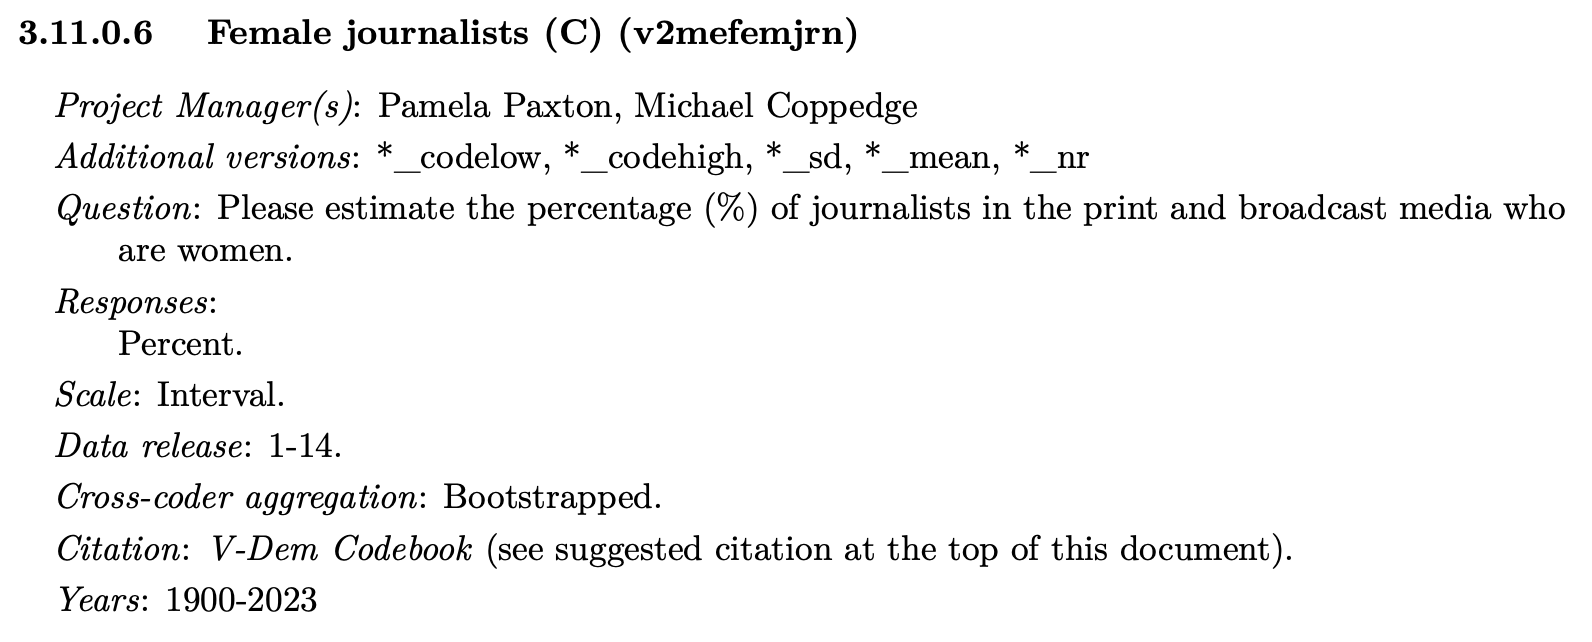
\includegraphics[width=1\linewidth]{images/w8_vdemExample} \end{center}

\begin{Shaded}
\begin{Highlighting}[]
\FunctionTok{head}\NormalTok{(vdem\_selected}\SpecialCharTok{$}\NormalTok{v2mefemjrn)}
\end{Highlighting}
\end{Shaded}

\begin{verbatim}
## [1] 36.857 39.000 50.294 40.167 36.406 42.688
\end{verbatim}

\begin{Shaded}
\begin{Highlighting}[]
\FunctionTok{cut}\NormalTok{(vdem\_selected}\SpecialCharTok{$}\NormalTok{v2mefemjrn, }\CommentTok{\# numeric variable}
    \AttributeTok{breaks=}\DecValTok{4}\NormalTok{) }\SpecialCharTok{|\textgreater{}} \CommentTok{\# either number of intervals OR list of cut points}
  \FunctionTok{head}\NormalTok{()}
\end{Highlighting}
\end{Shaded}

\begin{verbatim}
## [1] (24.4,38.5] (38.5,52.5] (38.5,52.5] (38.5,52.5] (24.4,38.5] (38.5,52.5]
## Levels: (10.3,24.4] (24.4,38.5] (38.5,52.5] (52.5,66.7]
\end{verbatim}

\begin{Shaded}
\begin{Highlighting}[]
\FunctionTok{cut}\NormalTok{(vdem\_selected}\SpecialCharTok{$}\NormalTok{v2mefemjrn, }\CommentTok{\# numeric variable}
    \AttributeTok{breaks=}\FunctionTok{c}\NormalTok{(}\DecValTok{10}\NormalTok{,}\DecValTok{30}\NormalTok{,}\DecValTok{50}\NormalTok{,}\DecValTok{70}\NormalTok{)) }\SpecialCharTok{|\textgreater{}} \CommentTok{\# either number of intervals OR list of cut points}
  \FunctionTok{head}\NormalTok{()}
\end{Highlighting}
\end{Shaded}

\begin{verbatim}
## [1] (30,50] (30,50] (50,70] (30,50] (30,50] (30,50]
## Levels: (10,30] (30,50] (50,70]
\end{verbatim}

\subsubsection*{Create a new dataframe with new ordinal variables}\label{create-a-new-dataframe-with-new-ordinal-variables}
\addcontentsline{toc}{subsubsection}{Create a new dataframe with new ordinal variables}

\begin{Shaded}
\begin{Highlighting}[]
\NormalTok{crosstab }\OtherTok{\textless{}{-}}\NormalTok{ vdem\_selected }\SpecialCharTok{|\textgreater{}}
  \FunctionTok{mutate}\NormalTok{(}\AttributeTok{v2mefemjrn\_ord4 =} \FunctionTok{cut}\NormalTok{(v2mefemjrn, }
                              \AttributeTok{breaks =} \DecValTok{4}\NormalTok{),}
         \AttributeTok{v2pepwrgen\_ord4 =} \FunctionTok{cut}\NormalTok{(v2pepwrgen, }
                                 \AttributeTok{breaks =} \DecValTok{4}\NormalTok{))}
\end{Highlighting}
\end{Shaded}

\subsubsection*{Crosstabs}\label{crosstabs}
\addcontentsline{toc}{subsubsection}{Crosstabs}

\begin{Shaded}
\begin{Highlighting}[]
\FunctionTok{tab\_xtab}\NormalTok{(}\AttributeTok{var.row =}\NormalTok{ crosstab}\SpecialCharTok{$}\NormalTok{v2mefemjrn\_ord4,}
         \AttributeTok{var.col =}\NormalTok{ crosstab}\SpecialCharTok{$}\NormalTok{v2pepwrgen\_ord4,}
         \AttributeTok{show.col.prc =} \ConstantTok{TRUE}\NormalTok{)}
\end{Highlighting}
\end{Shaded}

v2mefemjrn\_ord4

v2pepwrgen\_ord4

Total

(-1.97,-0.622{]}

(-0.622,0.724{]}

(0.724,2.07{]}

(2.07,3.42{]}

(10.3,24.4{]}

{8}{50~\%}

{8}{18.6~\%}

{11}{11.5~\%}

{1}{4.3~\%}

{28}{15.7~\%}

(24.4,38.5{]}

{7}{43.8~\%}

{22}{51.2~\%}

{37}{38.5~\%}

{2}{8.7~\%}

{68}{38.2~\%}

(38.5,52.5{]}

{1}{6.2~\%}

{11}{25.6~\%}

{40}{41.7~\%}

{18}{78.3~\%}

{70}{39.3~\%}

(52.5,66.7{]}

{0}{0~\%}

{2}{4.7~\%}

{8}{8.3~\%}

{2}{8.7~\%}

{12}{6.7~\%}

Total

{16}{100~\%}

{43}{100~\%}

{96}{100~\%}

{23}{100~\%}

{178}{100~\%}

χ2=39.809 · df=9 · Cramer's V=0.273 · Fisher's p=0.000

\subsubsection*{Export table}\label{export-table}
\addcontentsline{toc}{subsubsection}{Export table}

\begin{Shaded}
\begin{Highlighting}[]
\FunctionTok{tab\_xtab}\NormalTok{(}\AttributeTok{var.row =}\NormalTok{ crosstab}\SpecialCharTok{$}\NormalTok{v2mefemjrn\_ord4,}
         \AttributeTok{var.col =}\NormalTok{ crosstab}\SpecialCharTok{$}\NormalTok{v2pepwrgen\_ord4,}
         \AttributeTok{show.col.prc =} \ConstantTok{TRUE}\NormalTok{,}
         \AttributeTok{file=}\StringTok{"crosstabs.html"}\NormalTok{)}
\end{Highlighting}
\end{Shaded}

v2mefemjrn\_ord4

v2pepwrgen\_ord4

Total

(-1.97,-0.622{]}

(-0.622,0.724{]}

(0.724,2.07{]}

(2.07,3.42{]}

(10.3,24.4{]}

{8}{50~\%}

{8}{18.6~\%}

{11}{11.5~\%}

{1}{4.3~\%}

{28}{15.7~\%}

(24.4,38.5{]}

{7}{43.8~\%}

{22}{51.2~\%}

{37}{38.5~\%}

{2}{8.7~\%}

{68}{38.2~\%}

(38.5,52.5{]}

{1}{6.2~\%}

{11}{25.6~\%}

{40}{41.7~\%}

{18}{78.3~\%}

{70}{39.3~\%}

(52.5,66.7{]}

{0}{0~\%}

{2}{4.7~\%}

{8}{8.3~\%}

{2}{8.7~\%}

{12}{6.7~\%}

Total

{16}{100~\%}

{43}{100~\%}

{96}{100~\%}

{23}{100~\%}

{178}{100~\%}

χ2=39.809 · df=9 · Cramer's V=0.273 · Fisher's p=0.000

For your final project, open the html file on your laptops and copy the table into your word document

\subsection*{Skewed variables}\label{skewed-variables}
\addcontentsline{toc}{subsection}{Skewed variables}

\begin{Shaded}
\begin{Highlighting}[]
\FunctionTok{ggplot}\NormalTok{(vdem\_selected,}\FunctionTok{aes}\NormalTok{(}\AttributeTok{x=}\NormalTok{e\_gdppc)) }\SpecialCharTok{+}
  \FunctionTok{geom\_histogram}\NormalTok{()}
\end{Highlighting}
\end{Shaded}

\pandocbounded{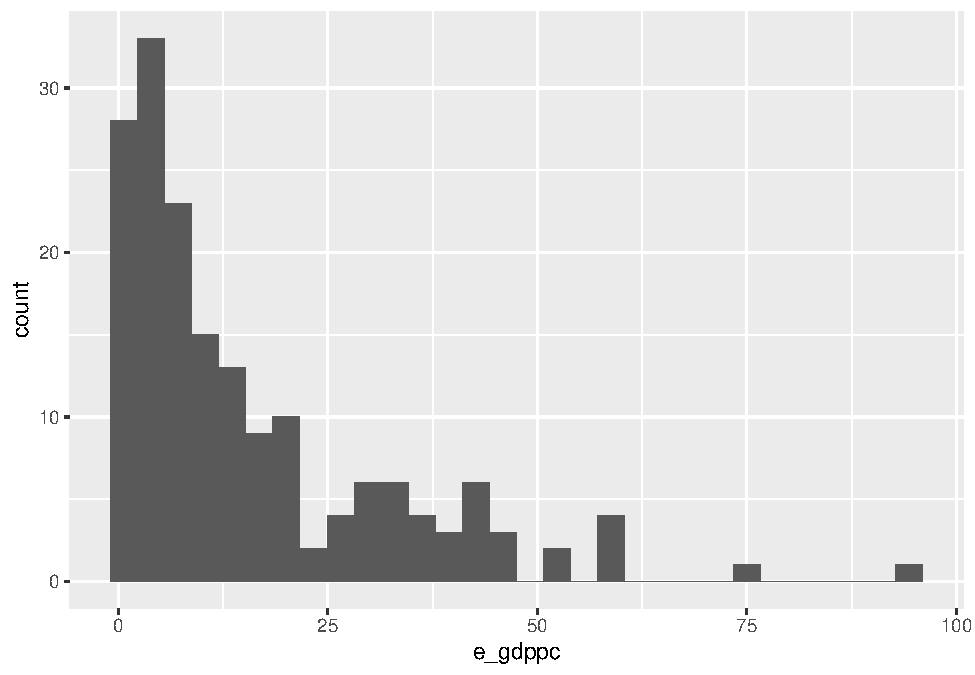
\includegraphics[keepaspectratio]{POL342-tutorial-notes_files/figure-latex/unnamed-chunk-232-1.pdf}}

\subsubsection*{Crosstabs will not display well}\label{crosstabs-will-not-display-well}
\addcontentsline{toc}{subsubsection}{Crosstabs will not display well}

\begin{Shaded}
\begin{Highlighting}[]
\NormalTok{crosstab2 }\OtherTok{\textless{}{-}}\NormalTok{ vdem\_selected }\SpecialCharTok{|\textgreater{}}
  \FunctionTok{mutate}\NormalTok{(}\AttributeTok{e\_gdppc\_ord4 =} \FunctionTok{cut}\NormalTok{(e\_gdppc, }
                            \AttributeTok{breaks =} \DecValTok{4}\NormalTok{),}
         \AttributeTok{v2x\_libdem\_ord4 =} \FunctionTok{cut}\NormalTok{(v2x\_libdem, }
                          \AttributeTok{breaks =} \DecValTok{4}\NormalTok{))}

\FunctionTok{tab\_xtab}\NormalTok{(}\AttributeTok{var.row =}\NormalTok{ crosstab2}\SpecialCharTok{$}\NormalTok{e\_gdppc\_ord4,}
         \AttributeTok{var.col =}\NormalTok{ crosstab2}\SpecialCharTok{$}\NormalTok{v2x\_libdem\_ord4,}
         \AttributeTok{show.col.prc =} \ConstantTok{TRUE}\NormalTok{)}
\end{Highlighting}
\end{Shaded}

e\_gdppc\_ord4

v2x\_libdem\_ord4

Total

(0.00411,0.227{]}

(0.227,0.45{]}

(0.45,0.672{]}

(0.672,0.895{]}

(0.577,24.1{]}

{49}{89.1~\%}

{44}{95.7~\%}

{29}{90.6~\%}

{11}{27.5~\%}

{133}{76.9~\%}

(24.1,47.5{]}

{4}{7.3~\%}

{0}{0~\%}

{3}{9.4~\%}

{25}{62.5~\%}

{32}{18.5~\%}

(47.5,71{]}

{1}{1.8~\%}

{2}{4.3~\%}

{0}{0~\%}

{3}{7.5~\%}

{6}{3.5~\%}

(71,94.5{]}

{1}{1.8~\%}

{0}{0~\%}

{0}{0~\%}

{1}{2.5~\%}

{2}{1.2~\%}

Total

{55}{100~\%}

{46}{100~\%}

{32}{100~\%}

{40}{100~\%}

{173}{100~\%}

χ2=77.469 · df=9 · Cramer's V=0.386 · Fisher's p=0.000

\subsubsection*{Alternative using quantile cut points}\label{alternative-using-quantile-cut-points}
\addcontentsline{toc}{subsubsection}{Alternative using quantile cut points}

\begin{Shaded}
\begin{Highlighting}[]
\FunctionTok{quantile}\NormalTok{(vdem\_selected}\SpecialCharTok{$}\NormalTok{e\_gdppc, }\AttributeTok{probs =} \FunctionTok{seq}\NormalTok{(}\DecValTok{0}\NormalTok{, }\DecValTok{1}\NormalTok{, }\FloatTok{0.25}\NormalTok{),}\AttributeTok{na.rm=}\NormalTok{T)}
\end{Highlighting}
\end{Shaded}

\begin{verbatim}
##     0%    25%    50%    75%   100% 
##  0.671  3.315  8.971 20.720 94.400
\end{verbatim}

\begin{Shaded}
\begin{Highlighting}[]
\NormalTok{crosstab3 }\OtherTok{\textless{}{-}}\NormalTok{ vdem\_selected }\SpecialCharTok{|\textgreater{}}
  \FunctionTok{mutate}\NormalTok{(}\AttributeTok{e\_gdppc\_ord4 =} \FunctionTok{cut}\NormalTok{(e\_gdppc, }
                            \AttributeTok{breaks =} \FunctionTok{quantile}\NormalTok{(e\_gdppc, }\AttributeTok{probs =} \FunctionTok{seq}\NormalTok{(}\DecValTok{0}\NormalTok{, }\DecValTok{1}\NormalTok{, }\FloatTok{0.25}\NormalTok{),}\AttributeTok{na.rm=}\NormalTok{T)),}
         \AttributeTok{v2x\_libdem\_ord4 =} \FunctionTok{cut}\NormalTok{(v2x\_libdem, }
                               \AttributeTok{breaks =} \FunctionTok{quantile}\NormalTok{(v2x\_libdem, }\AttributeTok{probs =} \FunctionTok{seq}\NormalTok{(}\DecValTok{0}\NormalTok{, }\DecValTok{1}\NormalTok{, }\FloatTok{0.25}\NormalTok{),}\AttributeTok{na.rm=}\NormalTok{T)))}

\FunctionTok{tab\_xtab}\NormalTok{(}\AttributeTok{var.row =}\NormalTok{ crosstab3}\SpecialCharTok{$}\NormalTok{v2x\_libdem\_ord4,}
         \AttributeTok{var.col =}\NormalTok{ crosstab3}\SpecialCharTok{$}\NormalTok{e\_gdppc\_ord4,}
         \AttributeTok{show.col.prc =} \ConstantTok{TRUE}\NormalTok{)}
\end{Highlighting}
\end{Shaded}

v2x\_libdem\_ord4

e\_gdppc\_ord4

Total

(0.671,3.31{]}

(3.31,8.97{]}

(8.97,20.7{]}

(20.7,94.4{]}

(0.005,0.157{]}

{12}{27.9~\%}

{13}{30.2~\%}

{9}{21.4~\%}

{7}{16.3~\%}

{41}{24~\%}

(0.157,0.373{]}

{18}{41.9~\%}

{12}{27.9~\%}

{9}{21.4~\%}

{2}{4.7~\%}

{41}{24~\%}

(0.373,0.66{]}

{13}{30.2~\%}

{15}{34.9~\%}

{13}{31~\%}

{3}{7~\%}

{44}{25.7~\%}

(0.66,0.894{]}

{0}{0~\%}

{3}{7~\%}

{11}{26.2~\%}

{31}{72.1~\%}

{45}{26.3~\%}

Total

{43}{100~\%}

{43}{100~\%}

{42}{100~\%}

{43}{100~\%}

{171}{100~\%}

χ2=74.710 · df=9 · Cramer's V=0.382 · p=0.000

\chapter{Communicating results}\label{communicating-results}

\begin{itemize}
\tightlist
\item
  Goals for today's class:

  \begin{itemize}
  \tightlist
  \item
    Regression tables
  \item
    Save tables and figures
  \end{itemize}
\end{itemize}

\section{Set-up}\label{set-up-2}

\section{Load libraries}\label{load-libraries-2}

\begin{Shaded}
\begin{Highlighting}[]
\FunctionTok{library}\NormalTok{(tidyverse)}
\FunctionTok{library}\NormalTok{(haven)}

\FunctionTok{install.packages}\NormalTok{(}\StringTok{"modelsummary"}\NormalTok{) }\CommentTok{\# regression table}
\FunctionTok{install.packages}\NormalTok{(}\StringTok{"pandoc"}\NormalTok{) }\CommentTok{\# to save regression table to Word doc output}
\FunctionTok{library}\NormalTok{(modelsummary)}
\end{Highlighting}
\end{Shaded}

\section{VDem}\label{vdem-2}

\begin{Shaded}
\begin{Highlighting}[]
\NormalTok{vars }\OtherTok{\textless{}{-}} \FunctionTok{c}\NormalTok{(}\StringTok{"country\_name"}\NormalTok{, }\StringTok{"country\_id"}\NormalTok{, }\StringTok{"year"}\NormalTok{, }
          \StringTok{"v2x\_corr"}\NormalTok{,}\StringTok{"e\_gdppc"}\NormalTok{)}

\NormalTok{df }\OtherTok{\textless{}{-}} \FunctionTok{read.csv}\NormalTok{(}\StringTok{"Project/VDem/VDem\_post2000.csv"}\NormalTok{) }\SpecialCharTok{|\textgreater{}}
\NormalTok{  dplyr}\SpecialCharTok{::}\FunctionTok{select}\NormalTok{(}\FunctionTok{all\_of}\NormalTok{(vars)) }\SpecialCharTok{|\textgreater{}}
  \FunctionTok{filter}\NormalTok{(year}\SpecialCharTok{==}\DecValTok{2009}\NormalTok{) }
\end{Highlighting}
\end{Shaded}

\subsection*{Scatter plot the bivariate relationship}\label{scatter-plot-the-bivariate-relationship}
\addcontentsline{toc}{subsection}{Scatter plot the bivariate relationship}

\begin{Shaded}
\begin{Highlighting}[]
\FunctionTok{ggplot}\NormalTok{(}\AttributeTok{data=}\NormalTok{df,}\FunctionTok{aes}\NormalTok{(}\AttributeTok{x=}\NormalTok{v2x\_corr,}\AttributeTok{y=}\NormalTok{e\_gdppc)) }\SpecialCharTok{+}
  \FunctionTok{geom\_point}\NormalTok{()}
\end{Highlighting}
\end{Shaded}

\pandocbounded{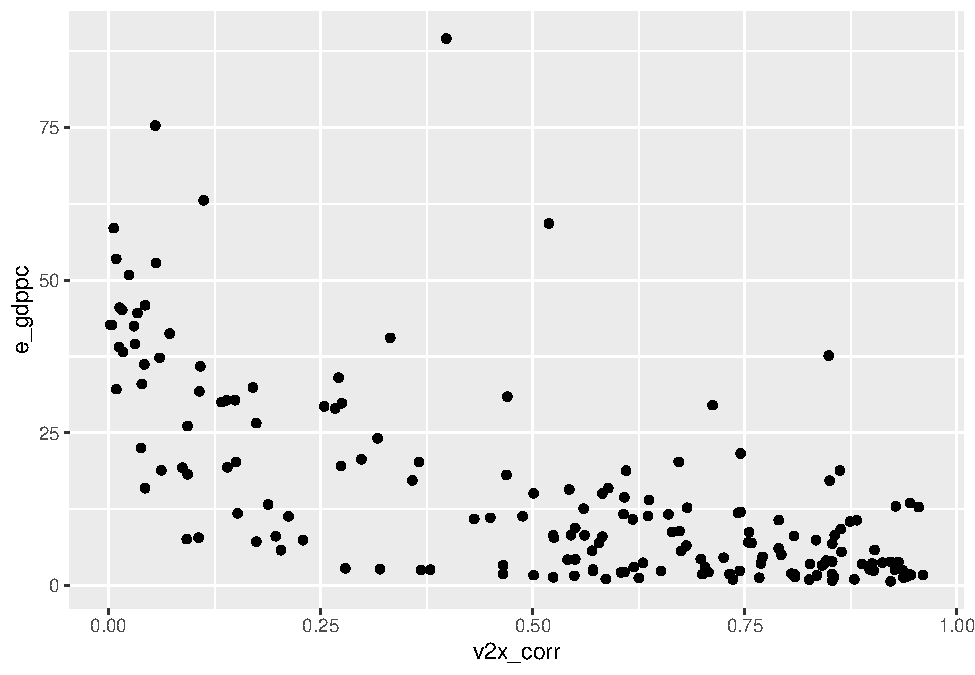
\includegraphics[keepaspectratio]{POL342-tutorial-notes_files/figure-latex/unnamed-chunk-239-1.pdf}}

\subsection*{Regression line}\label{regression-line}
\addcontentsline{toc}{subsection}{Regression line}

\begin{Shaded}
\begin{Highlighting}[]
\FunctionTok{ggplot}\NormalTok{(}\AttributeTok{data=}\NormalTok{df,}\FunctionTok{aes}\NormalTok{(}\AttributeTok{x=}\NormalTok{v2x\_corr,}\AttributeTok{y=}\NormalTok{e\_gdppc)) }\SpecialCharTok{+}
  \FunctionTok{geom\_point}\NormalTok{(}\AttributeTok{size=}\DecValTok{1}\NormalTok{,}\AttributeTok{alpha=}\NormalTok{.}\DecValTok{5}\NormalTok{) }\SpecialCharTok{+}
  \FunctionTok{geom\_smooth}\NormalTok{(}\AttributeTok{method=}\StringTok{"lm"}\NormalTok{,}\AttributeTok{size=}\NormalTok{.}\DecValTok{5}\NormalTok{) }\SpecialCharTok{+} \CommentTok{\# linear model, i.e. linear regression}
  \FunctionTok{scale\_y\_continuous}\NormalTok{(}\AttributeTok{breaks=}\FunctionTok{c}\NormalTok{(}\FunctionTok{seq}\NormalTok{(}\SpecialCharTok{{-}}\DecValTok{5}\NormalTok{,}\DecValTok{100}\NormalTok{,}\AttributeTok{by=}\DecValTok{10}\NormalTok{)))}
\end{Highlighting}
\end{Shaded}

\pandocbounded{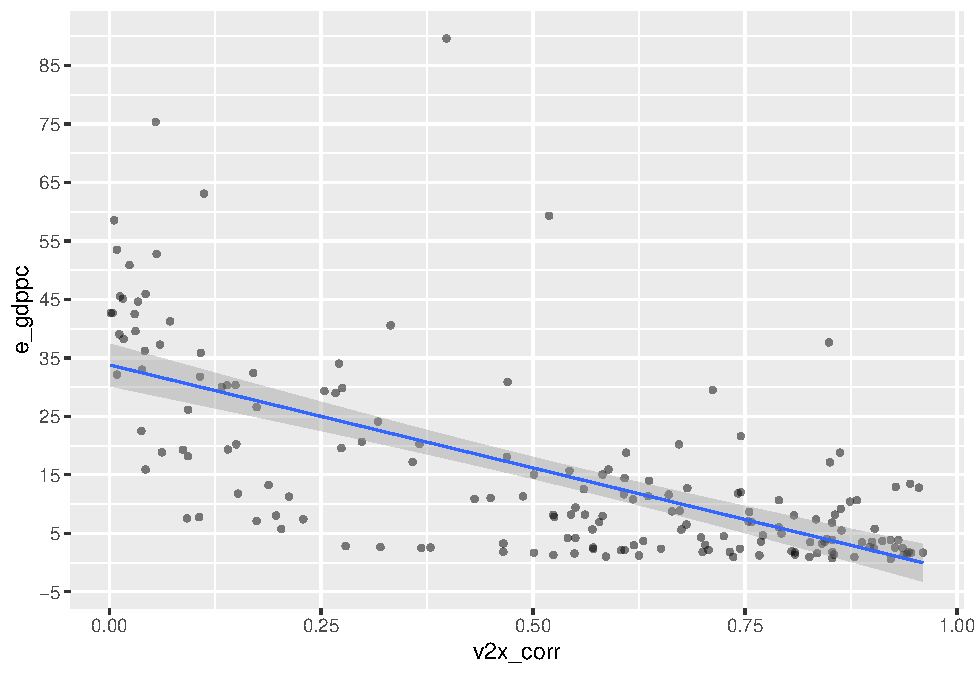
\includegraphics[keepaspectratio]{POL342-tutorial-notes_files/figure-latex/unnamed-chunk-240-1.pdf}}

\subsubsection*{Save ggplot as object}\label{save-ggplot-as-object}
\addcontentsline{toc}{subsubsection}{Save ggplot as object}

\begin{Shaded}
\begin{Highlighting}[]
\NormalTok{obj1 }\OtherTok{\textless{}{-}} \FunctionTok{ggplot}\NormalTok{(}\AttributeTok{data=}\NormalTok{df,}\FunctionTok{aes}\NormalTok{(}\AttributeTok{x=}\NormalTok{v2x\_corr,}\AttributeTok{y=}\NormalTok{e\_gdppc)) }\SpecialCharTok{+} \CommentTok{\# assign ggplot to obj1}
  \FunctionTok{geom\_point}\NormalTok{(}\AttributeTok{size=}\DecValTok{1}\NormalTok{,}\AttributeTok{alpha=}\NormalTok{.}\DecValTok{5}\NormalTok{) }\SpecialCharTok{+}
  \FunctionTok{geom\_smooth}\NormalTok{(}\AttributeTok{method=}\StringTok{"lm"}\NormalTok{,}\AttributeTok{size=}\NormalTok{.}\DecValTok{5}\NormalTok{) }\SpecialCharTok{+} \CommentTok{\# linear model, i.e. linear regression}
  \FunctionTok{scale\_y\_continuous}\NormalTok{(}\AttributeTok{breaks=}\FunctionTok{c}\NormalTok{(}\FunctionTok{seq}\NormalTok{(}\SpecialCharTok{{-}}\DecValTok{5}\NormalTok{,}\DecValTok{100}\NormalTok{,}\AttributeTok{by=}\DecValTok{10}\NormalTok{)))}
\end{Highlighting}
\end{Shaded}

\subsubsection*{\texorpdfstring{Using \texttt{ggsave}}{Using ggsave}}\label{using-ggsave}
\addcontentsline{toc}{subsubsection}{Using \texttt{ggsave}}

\begin{Shaded}
\begin{Highlighting}[]
\CommentTok{\# specify arguments \textasciigrave{}filename\textasciigrave{}, \textasciigrave{}plot\textasciigrave{}, \textasciigrave{}width\textasciigrave{} and \textasciigrave{}height\textasciigrave{} of image file}
\FunctionTok{ggsave}\NormalTok{(}\AttributeTok{filename =} \StringTok{"regressionLine.png"}\NormalTok{,}
       \AttributeTok{plot =}\NormalTok{ obj1,}
       \AttributeTok{width=}\DecValTok{8}\NormalTok{, }\AttributeTok{height=}\DecValTok{5}\NormalTok{)}
\end{Highlighting}
\end{Shaded}

\subsection*{Regression table}\label{regression-table}
\addcontentsline{toc}{subsection}{Regression table}

\subsubsection*{Regression output}\label{regression-output-1}
\addcontentsline{toc}{subsubsection}{Regression output}

\begin{Shaded}
\begin{Highlighting}[]
\NormalTok{m }\OtherTok{\textless{}{-}} \FunctionTok{lm}\NormalTok{(}\AttributeTok{data=}\NormalTok{df,e\_gdppc }\SpecialCharTok{\textasciitilde{}}\NormalTok{ v2x\_corr)}

\FunctionTok{summary}\NormalTok{(m)}
\end{Highlighting}
\end{Shaded}

\begin{verbatim}
## 
## Call:
## lm(formula = e_gdppc ~ v2x_corr, data = df)
## 
## Residuals:
##     Min      1Q  Median      3Q     Max 
## -23.003  -6.723  -0.466   4.466  69.824 
## 
## Coefficients:
##             Estimate Std. Error t value Pr(>|t|)    
## (Intercept)   33.817      1.828   18.50   <2e-16 ***
## v2x_corr     -35.263      3.008  -11.72   <2e-16 ***
## ---
## Signif. codes:  0 '***' 0.001 '**' 0.01 '*' 0.05 '.' 0.1 ' ' 1
## 
## Residual standard error: 12.22 on 171 degrees of freedom
##   (5 observations deleted due to missingness)
## Multiple R-squared:  0.4456, Adjusted R-squared:  0.4424 
## F-statistic: 137.4 on 1 and 171 DF,  p-value: < 2.2e-16
\end{verbatim}

\subsubsection*{\texorpdfstring{Table using \texttt{modelsummary}}{Table using modelsummary}}\label{table-using-modelsummary}
\addcontentsline{toc}{subsubsection}{Table using \texttt{modelsummary}}

\begin{Shaded}
\begin{Highlighting}[]
\FunctionTok{modelsummary}\NormalTok{(m, }\AttributeTok{stars=}\ConstantTok{TRUE}\NormalTok{)}
\end{Highlighting}
\end{Shaded}

\begin{table}
\centering
\begin{talltblr}[         %% tabularray outer open
entry=none,label=none,
note{}={+ p \num{< 0.1}, * p \num{< 0.05}, ** p \num{< 0.01}, *** p \num{< 0.001}},
]                     %% tabularray outer close
{                     %% tabularray inner open
colspec={Q[]Q[]},
hline{2}={1-2}{solid, black, 0.05em},
hline{6}={1-2}{solid, black, 0.05em},
hline{1}={1-2}{solid, black, 0.08em},
hline{13}={1-2}{solid, black, 0.08em},
column{2}={}{halign=c},
column{1}={}{halign=l},
}                     %% tabularray inner close
& (1) \\
(Intercept) & \num{33.817}*** \\
& (\num{1.828}) \\
v2x\_corr & \num{-35.263}*** \\
& (\num{3.008}) \\
Num.Obs. & \num{173} \\
R2 & \num{0.446} \\
R2 Adj. & \num{0.442} \\
AIC & \num{1360.9} \\
BIC & \num{1370.3} \\
Log.Lik. & \num{-677.441} \\
RMSE & \num{12.14} \\
\end{talltblr}
\end{table}

\subsubsection*{Goodness-of-fit statistics}\label{goodness-of-fit-statistics}
\addcontentsline{toc}{subsubsection}{Goodness-of-fit statistics}

\begin{Shaded}
\begin{Highlighting}[]
\FunctionTok{get\_gof}\NormalTok{(m)}
\end{Highlighting}
\end{Shaded}

\begin{verbatim}
##        aic      bic r.squared adj.r.squared     rmse nobs    logLik
## 1 1360.881 1370.341 0.4455993     0.4423572 12.14483  173 -677.4406
\end{verbatim}

\subsubsection*{Select relevant statistics}\label{select-relevant-statistics}
\addcontentsline{toc}{subsubsection}{Select relevant statistics}

\begin{itemize}
\tightlist
\item
  Keep only ``number of observations'', ``R-squared'', and ``adjusted R-squared'' values
\end{itemize}

\begin{Shaded}
\begin{Highlighting}[]
\FunctionTok{modelsummary}\NormalTok{(m, }
             \AttributeTok{stars=}\ConstantTok{TRUE}\NormalTok{, }
             \AttributeTok{gof\_map=}\FunctionTok{c}\NormalTok{(}\StringTok{"nobs"}\NormalTok{,}\StringTok{"r.squared"}\NormalTok{,}\StringTok{"adj.r.squared"}\NormalTok{)) }\CommentTok{\# select relevant goodness{-}of{-}fit statistics}
\end{Highlighting}
\end{Shaded}

\begin{table}
\centering
\begin{talltblr}[         %% tabularray outer open
entry=none,label=none,
note{}={+ p \num{< 0.1}, * p \num{< 0.05}, ** p \num{< 0.01}, *** p \num{< 0.001}},
]                     %% tabularray outer close
{                     %% tabularray inner open
colspec={Q[]Q[]},
hline{2}={1-2}{solid, black, 0.05em},
hline{6}={1-2}{solid, black, 0.05em},
hline{1}={1-2}{solid, black, 0.08em},
hline{9}={1-2}{solid, black, 0.08em},
column{2}={}{halign=c},
column{1}={}{halign=l},
}                     %% tabularray inner close
& (1) \\
(Intercept) & \num{33.817}*** \\
& (\num{1.828}) \\
v2x\_corr & \num{-35.263}*** \\
& (\num{3.008}) \\
Num.Obs. & \num{173} \\
R2 & \num{0.446} \\
R2 Adj. & \num{0.442} \\
\end{talltblr}
\end{table}

\subsubsection*{Relabel}\label{relabel}
\addcontentsline{toc}{subsubsection}{Relabel}

\begin{Shaded}
\begin{Highlighting}[]
\FunctionTok{modelsummary}\NormalTok{(}\FunctionTok{list}\NormalTok{(}\StringTok{"Base"}\OtherTok{=}\NormalTok{m), }\CommentTok{\# list allows me to name the models}
             \AttributeTok{stars=}\ConstantTok{TRUE}\NormalTok{,}
             \AttributeTok{gof\_map=}\FunctionTok{c}\NormalTok{(}\StringTok{"nobs"}\NormalTok{,}\StringTok{"r.squared"}\NormalTok{,}\StringTok{"adj.r.squared"}\NormalTok{), }
             \AttributeTok{coef\_rename=}\FunctionTok{c}\NormalTok{(}\StringTok{"v2x\_corr"}\OtherTok{=}\StringTok{"Corruption Index"}\NormalTok{)) }\CommentTok{\# rename coefficient}
\end{Highlighting}
\end{Shaded}

\begin{table}
\centering
\begin{talltblr}[         %% tabularray outer open
entry=none,label=none,
note{}={+ p \num{< 0.1}, * p \num{< 0.05}, ** p \num{< 0.01}, *** p \num{< 0.001}},
]                     %% tabularray outer close
{                     %% tabularray inner open
colspec={Q[]Q[]},
hline{2}={1-2}{solid, black, 0.05em},
hline{6}={1-2}{solid, black, 0.05em},
hline{1}={1-2}{solid, black, 0.08em},
hline{9}={1-2}{solid, black, 0.08em},
column{2}={}{halign=c},
column{1}={}{halign=l},
}                     %% tabularray inner close
& Base \\
(Intercept) & \num{33.817}*** \\
& (\num{1.828}) \\
Corruption Index & \num{-35.263}*** \\
& (\num{3.008}) \\
Num.Obs. & \num{173} \\
R2 & \num{0.446} \\
R2 Adj. & \num{0.442} \\
\end{talltblr}
\end{table}

\subsubsection*{Save output}\label{save-output}
\addcontentsline{toc}{subsubsection}{Save output}

Under Arguments \textgreater{} output, you can see a number of supported file formats: .docx, .html, .tex, .md, .txt, .csv, .xlsx, .png, .jpg

\begin{Shaded}
\begin{Highlighting}[]
\NormalTok{?modelsummary}
\end{Highlighting}
\end{Shaded}

\begin{Shaded}
\begin{Highlighting}[]
\FunctionTok{modelsummary}\NormalTok{(}\FunctionTok{list}\NormalTok{(}\StringTok{"Base"}\OtherTok{=}\NormalTok{m),}
             \AttributeTok{stars=}\ConstantTok{TRUE}\NormalTok{,}
             \AttributeTok{gof\_map=}\FunctionTok{c}\NormalTok{(}\StringTok{"nobs"}\NormalTok{,}\StringTok{"r.squared"}\NormalTok{,}\StringTok{"adj.r.squared"}\NormalTok{), }
             \AttributeTok{coef\_rename=}\FunctionTok{c}\NormalTok{(}\StringTok{"v2x\_corr"}\OtherTok{=}\StringTok{"Corruption Index"}\NormalTok{),}
             \AttributeTok{output=}\StringTok{"out.docx"}\NormalTok{) }
\end{Highlighting}
\end{Shaded}

\subsection*{Clear environment}\label{clear-environment}
\addcontentsline{toc}{subsection}{Clear environment}

\begin{Shaded}
\begin{Highlighting}[]
\FunctionTok{rm}\NormalTok{(}\AttributeTok{list=}\FunctionTok{ls}\NormalTok{())}
\end{Highlighting}
\end{Shaded}

\section{Canadian Election Study 2021}\label{canadian-election-study-2021-1}

\begin{Shaded}
\begin{Highlighting}[]
\NormalTok{vars }\OtherTok{\textless{}{-}} \FunctionTok{c}\NormalTok{(}\StringTok{"cps21\_age"}\NormalTok{,}\StringTok{"cps21\_news\_cons"}\NormalTok{,}\StringTok{"cps21\_govt\_confusing"}\NormalTok{) }\CommentTok{\#news consumption and internal political efficacy}

\NormalTok{ces\_select }\OtherTok{\textless{}{-}} \FunctionTok{read\_dta}\NormalTok{(}\StringTok{"Project/CES2021/2021 Canadian Election Study v2.0.dta"}\NormalTok{) }\SpecialCharTok{|\textgreater{}}
\NormalTok{  dplyr}\SpecialCharTok{::}\FunctionTok{select}\NormalTok{(}\FunctionTok{all\_of}\NormalTok{(vars))}
\end{Highlighting}
\end{Shaded}

\subsection*{Transform \& drop NAs}\label{transform-drop-nas}
\addcontentsline{toc}{subsection}{Transform \& drop NAs}

\begin{Shaded}
\begin{Highlighting}[]
\NormalTok{ces\_dropna }\OtherTok{\textless{}{-}}\NormalTok{ ces\_select }\SpecialCharTok{|\textgreater{}}
  \FunctionTok{mutate}\NormalTok{(}\AttributeTok{cps21\_govt\_confusing=}\FunctionTok{ifelse}\NormalTok{(cps21\_govt\_confusing}\SpecialCharTok{==}\DecValTok{5}\NormalTok{, }\CommentTok{\#conditional statement}
                                     \ConstantTok{NA}\NormalTok{, }\CommentTok{\#if yes}
\NormalTok{                                     cps21\_govt\_confusing), }\CommentTok{\#if no}
         \AttributeTok{cps21\_news\_cons=}\FunctionTok{ifelse}\NormalTok{(cps21\_news\_cons}\SpecialCharTok{==}\DecValTok{7}\NormalTok{, }\CommentTok{\#conditional statement}
                                \ConstantTok{NA}\NormalTok{, }\CommentTok{\#if yes}
\NormalTok{                                cps21\_news\_cons)) }\SpecialCharTok{|\textgreater{}} \CommentTok{\#if no}
  \FunctionTok{na.omit}\NormalTok{() }\CommentTok{\#remove NAs}
\end{Highlighting}
\end{Shaded}

\subsection*{Check transformed variables}\label{check-transformed-variables}
\addcontentsline{toc}{subsection}{Check transformed variables}

\begin{Shaded}
\begin{Highlighting}[]
\FunctionTok{table}\NormalTok{(ces\_dropna}\SpecialCharTok{$}\NormalTok{cps21\_govt\_confusing)}
\end{Highlighting}
\end{Shaded}

\begin{verbatim}
## 
##    1    2    3    4 
## 3371 5905 8464 2651
\end{verbatim}

\begin{Shaded}
\begin{Highlighting}[]
\FunctionTok{table}\NormalTok{(ces\_dropna}\SpecialCharTok{$}\NormalTok{cps21\_news\_cons)}
\end{Highlighting}
\end{Shaded}

\begin{verbatim}
## 
##    1    2    3    4    5    6 
##  646 3017 4660 5771 4433 1864
\end{verbatim}

\subsection*{Regression table}\label{regression-table-1}
\addcontentsline{toc}{subsection}{Regression table}

\begin{Shaded}
\begin{Highlighting}[]
\NormalTok{m }\OtherTok{\textless{}{-}} \FunctionTok{lm}\NormalTok{(}\AttributeTok{data=}\NormalTok{ces\_dropna,cps21\_govt\_confusing }\SpecialCharTok{\textasciitilde{}}\NormalTok{ cps21\_news\_cons) }\CommentTok{\# model 1}

\FunctionTok{summary}\NormalTok{(m)}
\end{Highlighting}
\end{Shaded}

\begin{verbatim}
## 
## Call:
## lm(formula = cps21_govt_confusing ~ cps21_news_cons, data = ces_dropna)
## 
## Residuals:
##     Min      1Q  Median      3Q     Max 
## -2.0799 -0.6698  0.1252  0.5352  1.9452 
## 
## Coefficients:
##                  Estimate Std. Error t value Pr(>|t|)    
## (Intercept)      3.284876   0.019173  171.33   <2e-16 ***
## cps21_news_cons -0.205011   0.004803  -42.68   <2e-16 ***
## ---
## Signif. codes:  0 '***' 0.001 '**' 0.01 '*' 0.05 '.' 0.1 ' ' 1
## 
## Residual standard error: 0.8785 on 20389 degrees of freedom
## Multiple R-squared:  0.08203,    Adjusted R-squared:  0.08198 
## F-statistic:  1822 on 1 and 20389 DF,  p-value: < 2.2e-16
\end{verbatim}

\begin{Shaded}
\begin{Highlighting}[]
\FunctionTok{modelsummary}\NormalTok{(}\FunctionTok{list}\NormalTok{(}\StringTok{"Base"}\OtherTok{=}\NormalTok{m),}
             \AttributeTok{stars=}\ConstantTok{TRUE}\NormalTok{,}
             \AttributeTok{gof\_map=}\FunctionTok{c}\NormalTok{(}\StringTok{"nobs"}\NormalTok{,}\StringTok{"r.squared"}\NormalTok{,}\StringTok{"adj.r.squared"}\NormalTok{), }
             \AttributeTok{coef\_rename=}\FunctionTok{c}\NormalTok{(}\StringTok{"cps21\_news\_cons"}\OtherTok{=}\StringTok{"News Consumption"}\NormalTok{)) }
\end{Highlighting}
\end{Shaded}

\begin{table}
\centering
\begin{talltblr}[         %% tabularray outer open
entry=none,label=none,
note{}={+ p \num{< 0.1}, * p \num{< 0.05}, ** p \num{< 0.01}, *** p \num{< 0.001}},
]                     %% tabularray outer close
{                     %% tabularray inner open
colspec={Q[]Q[]},
hline{2}={1-2}{solid, black, 0.05em},
hline{6}={1-2}{solid, black, 0.05em},
hline{1}={1-2}{solid, black, 0.08em},
hline{9}={1-2}{solid, black, 0.08em},
column{2}={}{halign=c},
column{1}={}{halign=l},
}                     %% tabularray inner close
& Base \\
(Intercept) & \num{3.285}*** \\
& (\num{0.019}) \\
News Consumption & \num{-0.205}*** \\
& (\num{0.005}) \\
Num.Obs. & \num{20391} \\
R2 & \num{0.082} \\
R2 Adj. & \num{0.082} \\
\end{talltblr}
\end{table}

\subsubsection*{Controls}\label{controls}
\addcontentsline{toc}{subsubsection}{Controls}

\begin{Shaded}
\begin{Highlighting}[]
\NormalTok{m2 }\OtherTok{\textless{}{-}} \FunctionTok{lm}\NormalTok{(}\AttributeTok{data=}\NormalTok{ces\_dropna,cps21\_govt\_confusing }\SpecialCharTok{\textasciitilde{}}\NormalTok{ cps21\_news\_cons }\SpecialCharTok{+}\NormalTok{ cps21\_age) }\CommentTok{\# model 2}

\FunctionTok{modelsummary}\NormalTok{(}\FunctionTok{list}\NormalTok{(}\StringTok{"Base"} \OtherTok{=}\NormalTok{ m,}
                  \StringTok{"w/ Controls"} \OtherTok{=}\NormalTok{ m2),}
             \AttributeTok{stars=}\ConstantTok{TRUE}\NormalTok{,}
             \AttributeTok{gof\_map=}\FunctionTok{c}\NormalTok{(}\StringTok{"nobs"}\NormalTok{,}\StringTok{"r.squared"}\NormalTok{,}\StringTok{"adj.r.squared"}\NormalTok{), }
             \AttributeTok{coef\_rename=}\FunctionTok{c}\NormalTok{(}\StringTok{"cps21\_news\_cons"} \OtherTok{=} \StringTok{"News Consumption"}\NormalTok{,}
                           \StringTok{"cps21\_age"} \OtherTok{=} \StringTok{"Age"}\NormalTok{)) }
\end{Highlighting}
\end{Shaded}

\begin{table}
\centering
\begin{talltblr}[         %% tabularray outer open
entry=none,label=none,
note{}={+ p \num{< 0.1}, * p \num{< 0.05}, ** p \num{< 0.01}, *** p \num{< 0.001}},
]                     %% tabularray outer close
{                     %% tabularray inner open
colspec={Q[]Q[]Q[]},
hline{2}={1-3}{solid, black, 0.05em},
hline{8}={1-3}{solid, black, 0.05em},
hline{1}={1-3}{solid, black, 0.08em},
hline{11}={1-3}{solid, black, 0.08em},
column{2-3}={}{halign=c},
column{1}={}{halign=l},
}                     %% tabularray inner close
& Base & w/ Controls \\
(Intercept) & \num{3.285}*** & \num{3.313}*** \\
& (\num{0.019}) & (\num{0.023}) \\
News Consumption & \num{-0.205}*** & \num{-0.200}*** \\
& (\num{0.005}) & (\num{0.005}) \\
Age &  & \num{-0.001}* \\
&  & (\num{0.000}) \\
Num.Obs. & \num{20391} & \num{20391} \\
R2 & \num{0.082} & \num{0.082} \\
R2 Adj. & \num{0.082} & \num{0.082} \\
\end{talltblr}
\end{table}

\subsubsection*{Save output}\label{save-output-1}
\addcontentsline{toc}{subsubsection}{Save output}

\begin{Shaded}
\begin{Highlighting}[]
\FunctionTok{modelsummary}\NormalTok{(}\FunctionTok{list}\NormalTok{(}\StringTok{"Base"} \OtherTok{=}\NormalTok{ m,}
                  \StringTok{"w/ Controls"} \OtherTok{=}\NormalTok{ m2),}
             \AttributeTok{stars=}\ConstantTok{TRUE}\NormalTok{,}
             \AttributeTok{gof\_map=}\FunctionTok{c}\NormalTok{(}\StringTok{"nobs"}\NormalTok{,}\StringTok{"r.squared"}\NormalTok{,}\StringTok{"adj.r.squared"}\NormalTok{), }
             \AttributeTok{coef\_rename=}\FunctionTok{c}\NormalTok{(}\StringTok{"cps21\_news\_cons"} \OtherTok{=} \StringTok{"News Consumption"}\NormalTok{,}
                           \StringTok{"cps21\_age"} \OtherTok{=} \StringTok{"Age"}\NormalTok{),}
             \AttributeTok{output=}\StringTok{"ces.docx"}\NormalTok{) }
\end{Highlighting}
\end{Shaded}

\subsection*{Clear environment}\label{clear-environment-1}
\addcontentsline{toc}{subsection}{Clear environment}

\begin{Shaded}
\begin{Highlighting}[]
\FunctionTok{rm}\NormalTok{(}\AttributeTok{list=}\FunctionTok{ls}\NormalTok{())}
\end{Highlighting}
\end{Shaded}

\section{World Values Survey}\label{world-values-survey}

\begin{Shaded}
\begin{Highlighting}[]
\NormalTok{vars }\OtherTok{\textless{}{-}} \FunctionTok{c}\NormalTok{(}\StringTok{"B\_COUNTRY\_ALPHA"}\NormalTok{,}\StringTok{"Q73"}\NormalTok{,}\StringTok{"Q236"}\NormalTok{) }\CommentTok{\#confidence in parliament, experts versus government}

\NormalTok{df }\OtherTok{\textless{}{-}} \FunctionTok{read\_rds}\NormalTok{(}\StringTok{"Project/WVS/WVS\_Cross{-}National\_Wave\_7\_rds\_v6\_0.rds"}\NormalTok{) }\SpecialCharTok{|\textgreater{}}
  \FunctionTok{select}\NormalTok{(}\FunctionTok{all\_of}\NormalTok{(vars)) }\SpecialCharTok{|\textgreater{}}
  \FunctionTok{filter}\NormalTok{(B\_COUNTRY\_ALPHA}\SpecialCharTok{==}\StringTok{"CAN"}\NormalTok{) }\CommentTok{\# choice of country: Canada}
\end{Highlighting}
\end{Shaded}

\subsection*{Transform \& drop NAs}\label{transform-drop-nas-1}
\addcontentsline{toc}{subsection}{Transform \& drop NAs}

\begin{Shaded}
\begin{Highlighting}[]
\NormalTok{df\_recode }\OtherTok{\textless{}{-}}\NormalTok{ df }\SpecialCharTok{|\textgreater{}}
  \FunctionTok{mutate}\NormalTok{(}\AttributeTok{Q73=}\FunctionTok{ifelse}\NormalTok{(Q73}\SpecialCharTok{\textless{}}\DecValTok{0}\NormalTok{,}
                    \ConstantTok{NA}\NormalTok{,}
\NormalTok{                    Q73),}
         \AttributeTok{Q236=}\FunctionTok{ifelse}\NormalTok{(Q236}\SpecialCharTok{\textless{}}\DecValTok{0}\NormalTok{,}
                     \ConstantTok{NA}\NormalTok{,}
\NormalTok{                     Q236)) }\SpecialCharTok{|\textgreater{}}
  \FunctionTok{na.omit}\NormalTok{() }\CommentTok{\# drops all rows with NA values}
\end{Highlighting}
\end{Shaded}

\subsection*{Regression table}\label{regression-table-2}
\addcontentsline{toc}{subsection}{Regression table}

\begin{Shaded}
\begin{Highlighting}[]
\NormalTok{m }\OtherTok{\textless{}{-}} \FunctionTok{lm}\NormalTok{(}\AttributeTok{data=}\NormalTok{df\_recode,}
\NormalTok{        Q236 }\SpecialCharTok{\textasciitilde{}}\NormalTok{ Q73)}

\FunctionTok{summary}\NormalTok{(m)}
\end{Highlighting}
\end{Shaded}

\begin{verbatim}
## 
## Call:
## lm(formula = Q236 ~ Q73, data = df_recode)
## 
## Residuals:
##     Min      1Q  Median      3Q     Max 
## -1.4973 -0.4910 -0.4848  0.5152  1.5214 
## 
## Coefficients:
##             Estimate Std. Error t value Pr(>|t|)    
## (Intercept)  2.50351    0.04915  50.937   <2e-16 ***
## Q73         -0.00623    0.01812  -0.344    0.731    
## ---
## Signif. codes:  0 '***' 0.001 '**' 0.01 '*' 0.05 '.' 0.1 ' ' 1
## 
## Residual standard error: 0.8836 on 4016 degrees of freedom
## Multiple R-squared:  2.944e-05,  Adjusted R-squared:  -0.0002196 
## F-statistic: 0.1183 on 1 and 4016 DF,  p-value: 0.731
\end{verbatim}

\begin{Shaded}
\begin{Highlighting}[]
\FunctionTok{modelsummary}\NormalTok{(}\FunctionTok{list}\NormalTok{(}\StringTok{"Experts vs government"}\OtherTok{=}\NormalTok{m),}
             \AttributeTok{stars=}\ConstantTok{TRUE}\NormalTok{,}
             \AttributeTok{gof\_map=}\FunctionTok{c}\NormalTok{(}\StringTok{"nobs"}\NormalTok{,}\StringTok{"r.squared"}\NormalTok{,}\StringTok{"adj.r.squared"}\NormalTok{), }
             \AttributeTok{coef\_rename=}\FunctionTok{c}\NormalTok{(}\StringTok{"Q73"}\OtherTok{=}\StringTok{"Confidence in Parliament"}\NormalTok{),}
             \AttributeTok{output=}\StringTok{"wvs\_regTable.docx"}\NormalTok{) }
\end{Highlighting}
\end{Shaded}

\subsection{Clear environment}\label{clear-environment-2}

\begin{Shaded}
\begin{Highlighting}[]
\FunctionTok{rm}\NormalTok{(}\AttributeTok{list=}\FunctionTok{ls}\NormalTok{())}
\end{Highlighting}
\end{Shaded}

\section{Asian Barometer}\label{asian-barometer}

\begin{Shaded}
\begin{Highlighting}[]
\NormalTok{vars }\OtherTok{\textless{}{-}} \FunctionTok{c}\NormalTok{(}\StringTok{"country"}\NormalTok{,}\StringTok{"Year"}\NormalTok{,}
           \StringTok{"q175"}\NormalTok{,}\StringTok{"q169"}\NormalTok{)}

\NormalTok{df }\OtherTok{\textless{}{-}} \FunctionTok{read\_dta}\NormalTok{(}\StringTok{"Project/asianbarometer\_wave5/20230504\_W5\_merge\_15.dta"}\NormalTok{) }\SpecialCharTok{|\textgreater{}}
  \FunctionTok{select}\NormalTok{(}\FunctionTok{all\_of}\NormalTok{(vars)) }\SpecialCharTok{|\textgreater{}}
  \FunctionTok{filter}\NormalTok{(country}\SpecialCharTok{==}\DecValTok{11}\NormalTok{) }\CommentTok{\# Vietnam (refer to codebook)}
\end{Highlighting}
\end{Shaded}

\subsection*{Transform \& drop NAs}\label{transform-drop-nas-2}
\addcontentsline{toc}{subsection}{Transform \& drop NAs}

\begin{Shaded}
\begin{Highlighting}[]
\NormalTok{df\_recode }\OtherTok{\textless{}{-}}\NormalTok{ df }\SpecialCharTok{|\textgreater{}}
  \FunctionTok{mutate}\NormalTok{(}\AttributeTok{q169 =} \FunctionTok{ifelse}\NormalTok{(q169}\SpecialCharTok{\textless{}}\DecValTok{1} \SpecialCharTok{|}\NormalTok{ q169 }\SpecialCharTok{\textgreater{}} \DecValTok{4}\NormalTok{, }\ConstantTok{NA}\NormalTok{, q169),}
         \AttributeTok{q175 =} \FunctionTok{ifelse}\NormalTok{(q175}\SpecialCharTok{\textless{}}\DecValTok{1} \SpecialCharTok{|}\NormalTok{ q175 }\SpecialCharTok{\textgreater{}} \DecValTok{4}\NormalTok{, }\ConstantTok{NA}\NormalTok{, q175)) }\SpecialCharTok{|\textgreater{}}
  \FunctionTok{na.omit}\NormalTok{()}
\end{Highlighting}
\end{Shaded}

\subsection*{Regression table}\label{regression-table-3}
\addcontentsline{toc}{subsection}{Regression table}

\begin{Shaded}
\begin{Highlighting}[]
\NormalTok{m }\OtherTok{\textless{}{-}} \FunctionTok{lm}\NormalTok{(}\AttributeTok{data=}\NormalTok{df\_recode,}
\NormalTok{        q169 }\SpecialCharTok{\textasciitilde{}}\NormalTok{ q175)}

\FunctionTok{summary}\NormalTok{(m)}
\end{Highlighting}
\end{Shaded}

\begin{verbatim}
## 
## Call:
## lm(formula = q169 ~ q175, data = df_recode)
## 
## Residuals:
##     Min      1Q  Median      3Q     Max 
## -1.7626 -0.6000  0.2374  0.4000  1.4812 
## 
## Coefficients:
##             Estimate Std. Error t value Pr(>|t|)    
## (Intercept)  2.43754    0.08119  30.022   <2e-16 ***
## q175         0.08125    0.04164   1.951   0.0513 .  
## ---
## Signif. codes:  0 '***' 0.001 '**' 0.01 '*' 0.05 '.' 0.1 ' ' 1
## 
## Residual standard error: 0.86 on 1005 degrees of freedom
## Multiple R-squared:  0.003775,   Adjusted R-squared:  0.002783 
## F-statistic: 3.808 on 1 and 1005 DF,  p-value: 0.05129
\end{verbatim}

\begin{Shaded}
\begin{Highlighting}[]
\FunctionTok{modelsummary}\NormalTok{(}\FunctionTok{list}\NormalTok{(}\StringTok{"Views toward Democracy"}\OtherTok{=}\NormalTok{m),}
             \AttributeTok{stars=}\ConstantTok{TRUE}\NormalTok{,}
             \AttributeTok{gof\_map=}\FunctionTok{c}\NormalTok{(}\StringTok{"nobs"}\NormalTok{,}\StringTok{"r.squared"}\NormalTok{,}\StringTok{"adj.r.squared"}\NormalTok{), }
             \AttributeTok{coef\_rename=}\FunctionTok{c}\NormalTok{(}\StringTok{"q175"}\OtherTok{=}\StringTok{"US harm to Asia"}\NormalTok{),}
             \AttributeTok{output=}\StringTok{"AB\_regTable.docx"}\NormalTok{) }
\end{Highlighting}
\end{Shaded}

\subsection*{Saving plots}\label{saving-plots}
\addcontentsline{toc}{subsection}{Saving plots}

\begin{Shaded}
\begin{Highlighting}[]
\NormalTok{df\_recode }\SpecialCharTok{|\textgreater{}}
  \FunctionTok{ggplot}\NormalTok{(}\FunctionTok{aes}\NormalTok{(}\AttributeTok{fill=}\FunctionTok{factor}\NormalTok{(q169),}\AttributeTok{x=}\FunctionTok{factor}\NormalTok{(q175))) }\SpecialCharTok{+}
  \FunctionTok{geom\_bar}\NormalTok{(}\AttributeTok{position=}\StringTok{"fill"}\NormalTok{) }\SpecialCharTok{+}
  \FunctionTok{theme\_bw}\NormalTok{() }\SpecialCharTok{+}
  \FunctionTok{scale\_x\_discrete}\NormalTok{(}\AttributeTok{labels=}\FunctionTok{c}\NormalTok{(}\StringTok{"Much more good"}\NormalTok{,}\StringTok{"More good"}\NormalTok{, }\StringTok{"More harm"}\NormalTok{, }\StringTok{"Much more harm"}\NormalTok{)) }\SpecialCharTok{+}
  \FunctionTok{xlab}\NormalTok{(}\StringTok{"US does more good or harm to Asia?"}\NormalTok{) }\SpecialCharTok{+}
  \FunctionTok{ylab}\NormalTok{(}\StringTok{"Proportion"}\NormalTok{) }\SpecialCharTok{+}
  \FunctionTok{scale\_fill\_manual}\NormalTok{(}\AttributeTok{name=}\StringTok{"Democratic regimes full of problems"}\NormalTok{, }\CommentTok{\#legend label}
                    \AttributeTok{values =} \FunctionTok{c}\NormalTok{(}\StringTok{"navyblue"}\NormalTok{,}\StringTok{"blue"}\NormalTok{,}\StringTok{"skyblue"}\NormalTok{,}\StringTok{"grey"}\NormalTok{), }\CommentTok{\#color specification}
                    \AttributeTok{labels =} \FunctionTok{c}\NormalTok{(}\StringTok{"Strongly Agree"}\NormalTok{,}\StringTok{"Somewhat Agree"}\NormalTok{, }\StringTok{"Disagree"}\NormalTok{, }\StringTok{"Strongly Disagree"}\NormalTok{))}
\end{Highlighting}
\end{Shaded}

\pandocbounded{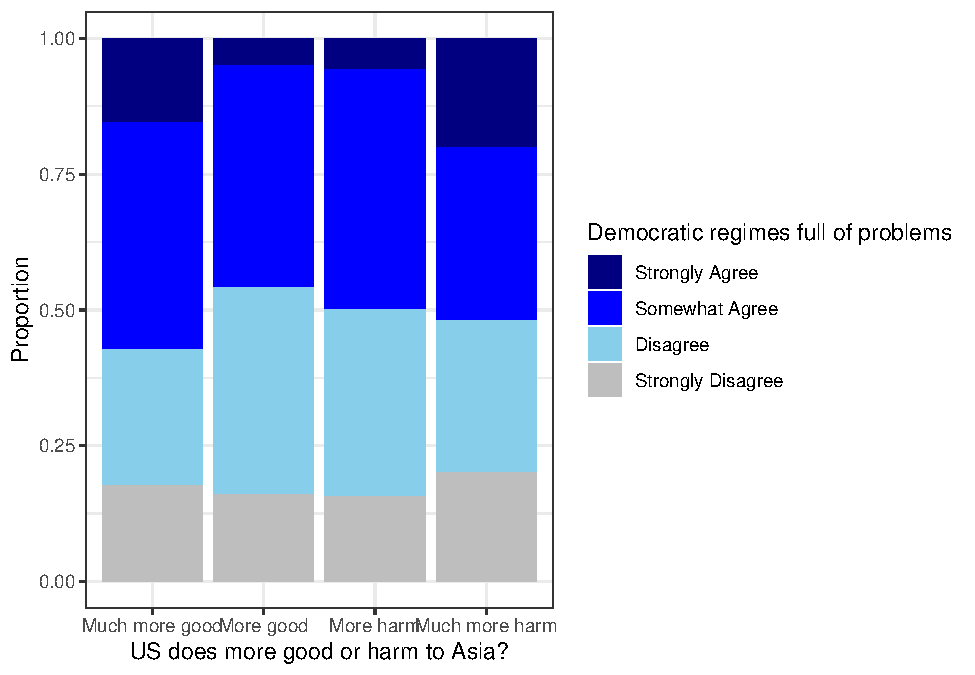
\includegraphics[keepaspectratio]{POL342-tutorial-notes_files/figure-latex/unnamed-chunk-265-1.pdf}}

\subsubsection*{Save ggplot as object}\label{save-ggplot-as-object-1}
\addcontentsline{toc}{subsubsection}{Save ggplot as object}

\begin{Shaded}
\begin{Highlighting}[]
\NormalTok{obj1 }\OtherTok{\textless{}{-}}\NormalTok{ df\_recode }\SpecialCharTok{|\textgreater{}}
  \FunctionTok{ggplot}\NormalTok{(}\FunctionTok{aes}\NormalTok{(}\AttributeTok{fill=}\FunctionTok{factor}\NormalTok{(q169),}\AttributeTok{x=}\FunctionTok{factor}\NormalTok{(q175))) }\SpecialCharTok{+}
  \FunctionTok{geom\_bar}\NormalTok{(}\AttributeTok{position=}\StringTok{"fill"}\NormalTok{) }\SpecialCharTok{+}
  \FunctionTok{theme\_bw}\NormalTok{() }\SpecialCharTok{+}
  \FunctionTok{scale\_x\_discrete}\NormalTok{(}\AttributeTok{labels=}\FunctionTok{c}\NormalTok{(}\StringTok{"Much more good"}\NormalTok{,}\StringTok{"More good"}\NormalTok{, }\StringTok{"More harm"}\NormalTok{, }\StringTok{"Much more harm"}\NormalTok{)) }\SpecialCharTok{+}
  \FunctionTok{xlab}\NormalTok{(}\StringTok{"US does more good or harm to Asia?"}\NormalTok{) }\SpecialCharTok{+}
  \FunctionTok{ylab}\NormalTok{(}\StringTok{"Proportion"}\NormalTok{) }\SpecialCharTok{+}
  \FunctionTok{scale\_fill\_manual}\NormalTok{(}\AttributeTok{name=}\StringTok{"Democratic regimes full of problems"}\NormalTok{, }\CommentTok{\#legend label}
                    \AttributeTok{values =} \FunctionTok{c}\NormalTok{(}\StringTok{"navyblue"}\NormalTok{,}\StringTok{"blue"}\NormalTok{,}\StringTok{"skyblue"}\NormalTok{,}\StringTok{"grey"}\NormalTok{), }\CommentTok{\#color specification}
                    \AttributeTok{labels =} \FunctionTok{c}\NormalTok{(}\StringTok{"Strongly Agree"}\NormalTok{,}\StringTok{"Somewhat Agree"}\NormalTok{, }\StringTok{"Disagree"}\NormalTok{, }\StringTok{"Strongly Disagree"}\NormalTok{))}
\end{Highlighting}
\end{Shaded}

\subsubsection*{\texorpdfstring{Using \texttt{ggsave}}{Using ggsave}}\label{using-ggsave-1}
\addcontentsline{toc}{subsubsection}{Using \texttt{ggsave}}

\begin{Shaded}
\begin{Highlighting}[]
\CommentTok{\# specify arguments filename and plot}
\FunctionTok{ggsave}\NormalTok{(}\AttributeTok{filename =} \StringTok{"AB\_x169y175.png"}\NormalTok{,}
       \AttributeTok{plot =}\NormalTok{ obj1,}
       \AttributeTok{height =} \DecValTok{5}\NormalTok{, }\AttributeTok{width =} \DecValTok{8}\NormalTok{)}
\end{Highlighting}
\end{Shaded}

\chapter{Optimizing ggplot presentation}\label{optimizing-ggplot-presentation}

\begin{itemize}
\tightlist
\item
  Goals for today's class:

  \begin{itemize}
  \tightlist
  \item
    Optimizing ggplot presentation for each of the plot types (bar charts, box and whiskers, scatter plot)
  \item
    Other graph specifications (themes, axes, font size, etc.)
  \end{itemize}
\end{itemize}

\section{Load libraries}\label{load-libraries-3}

\begin{Shaded}
\begin{Highlighting}[]
\FunctionTok{library}\NormalTok{(tidyverse)}
\FunctionTok{library}\NormalTok{(haven)}
\FunctionTok{library}\NormalTok{(marginaleffects)}
\end{Highlighting}
\end{Shaded}

\section{Bar charts}\label{bar-charts}

\subsection*{Prepare variables (Asian Barometer)}\label{prepare-variables-asian-barometer}
\addcontentsline{toc}{subsection}{Prepare variables (Asian Barometer)}

\begin{itemize}
\tightlist
\item
  Independent variable: Views toward the US

  \begin{itemize}
  \tightlist
  \item
    175 Does the United States do more good or harm to Asia?
  \end{itemize}
\item
  Dependent variable: Views toward democracy (1 strongly agree - 4 strongly disagree)

  \begin{itemize}
  \tightlist
  \item
    170 Democratic systems are not effective at maintaining order and stability
  \end{itemize}
\end{itemize}

\subsubsection*{Load data and select variables}\label{load-data-and-select-variables}
\addcontentsline{toc}{subsubsection}{Load data and select variables}

\begin{Shaded}
\begin{Highlighting}[]
\NormalTok{vars }\OtherTok{\textless{}{-}} \FunctionTok{c}\NormalTok{(}\StringTok{"country"}\NormalTok{,}\StringTok{"Year"}\NormalTok{,}
           \StringTok{"q170"}\NormalTok{,}\StringTok{"q175"}\NormalTok{)}

\NormalTok{df }\OtherTok{\textless{}{-}} \FunctionTok{read\_dta}\NormalTok{(}\StringTok{"Project/asianbarometer\_wave5/20230504\_W5\_merge\_15.dta"}\NormalTok{) }\SpecialCharTok{|\textgreater{}}
  \FunctionTok{select}\NormalTok{(}\FunctionTok{all\_of}\NormalTok{(vars)) }\SpecialCharTok{|\textgreater{}}
  \FunctionTok{filter}\NormalTok{(country}\SpecialCharTok{==}\DecValTok{11}\NormalTok{) }\CommentTok{\# Vietnam}
\end{Highlighting}
\end{Shaded}

\subsubsection*{Recode variables}\label{recode-variables}
\addcontentsline{toc}{subsubsection}{Recode variables}

\begin{Shaded}
\begin{Highlighting}[]
\NormalTok{df\_recode }\OtherTok{\textless{}{-}}\NormalTok{ df }\SpecialCharTok{|\textgreater{}}
  \FunctionTok{mutate}\NormalTok{(}\AttributeTok{q170 =} \FunctionTok{ifelse}\NormalTok{(q170}\SpecialCharTok{\textless{}}\DecValTok{1} \SpecialCharTok{|}\NormalTok{ q170 }\SpecialCharTok{\textgreater{}} \DecValTok{4}\NormalTok{, }\ConstantTok{NA}\NormalTok{, q170),}
         \AttributeTok{q175 =} \FunctionTok{ifelse}\NormalTok{(q175}\SpecialCharTok{\textless{}}\DecValTok{1} \SpecialCharTok{|}\NormalTok{ q175 }\SpecialCharTok{\textgreater{}} \DecValTok{4}\NormalTok{, }\ConstantTok{NA}\NormalTok{, q175)) }\SpecialCharTok{|\textgreater{}}
  \FunctionTok{na.omit}\NormalTok{()}
\end{Highlighting}
\end{Shaded}

\subsubsection*{Basic plot}\label{basic-plot}
\addcontentsline{toc}{subsubsection}{Basic plot}

\begin{Shaded}
\begin{Highlighting}[]
\NormalTok{df\_recode }\SpecialCharTok{|\textgreater{}}
  \FunctionTok{ggplot}\NormalTok{(}\FunctionTok{aes}\NormalTok{(}\AttributeTok{fill=}\FunctionTok{factor}\NormalTok{(q170),}\AttributeTok{x=}\FunctionTok{factor}\NormalTok{(q175))) }\SpecialCharTok{+}
  \FunctionTok{geom\_bar}\NormalTok{(}\AttributeTok{position=}\StringTok{"fill"}\NormalTok{)}
\end{Highlighting}
\end{Shaded}

\pandocbounded{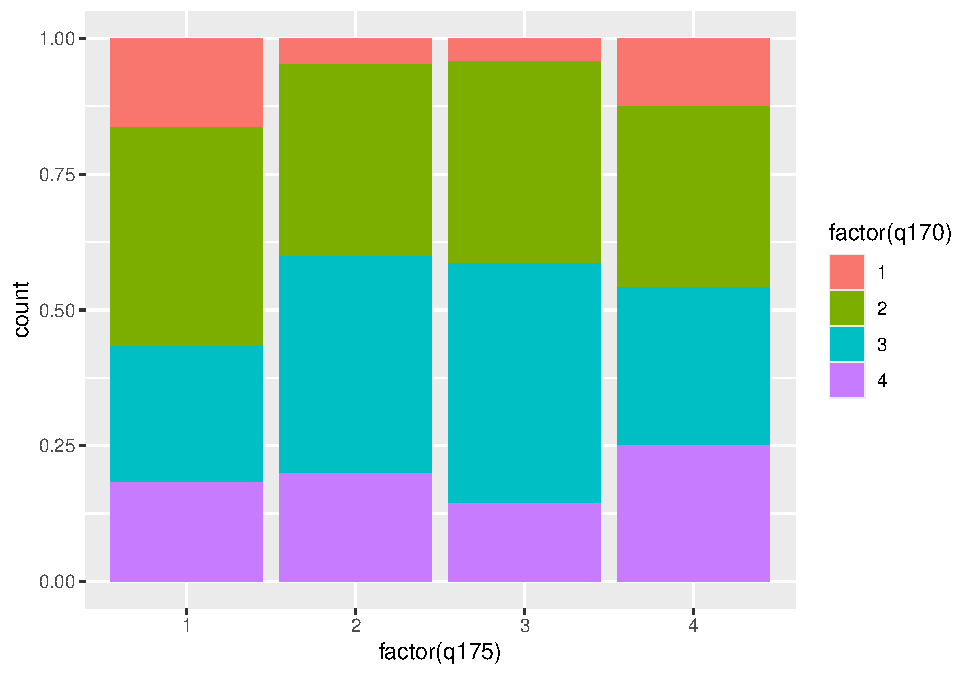
\includegraphics[keepaspectratio]{POL342-tutorial-notes_files/figure-latex/unnamed-chunk-273-1.pdf}}

\begin{itemize}
\tightlist
\item
  \texttt{theme\_bw()} -- changes the background theme
\item
  \texttt{scale\_fill\_manual} -- \texttt{name} to label legend title, \texttt{values} to change colors, \texttt{labels} to change name of levels
\item
  \texttt{scale\_x\_discrete} -- adjusts x-axis; \texttt{labels} to change name of levels; \texttt{guide} to stagger labels to prevent overlapping
\item
  \texttt{xlab} -- x-axis title
\item
  \texttt{ylab} -- y-axis title
\item
  \texttt{geom\_text} -- adds text annotation
\end{itemize}

\begin{Shaded}
\begin{Highlighting}[]
\NormalTok{df\_recode }\SpecialCharTok{|\textgreater{}}
  \FunctionTok{ggplot}\NormalTok{(}\FunctionTok{aes}\NormalTok{(}\AttributeTok{fill=}\FunctionTok{factor}\NormalTok{(q170),}\AttributeTok{x=}\FunctionTok{factor}\NormalTok{(q175))) }\SpecialCharTok{+}
  \FunctionTok{geom\_bar}\NormalTok{(}\AttributeTok{position=}\StringTok{"fill"}\NormalTok{) }\SpecialCharTok{+}
  \FunctionTok{theme\_bw}\NormalTok{()}
\end{Highlighting}
\end{Shaded}

\pandocbounded{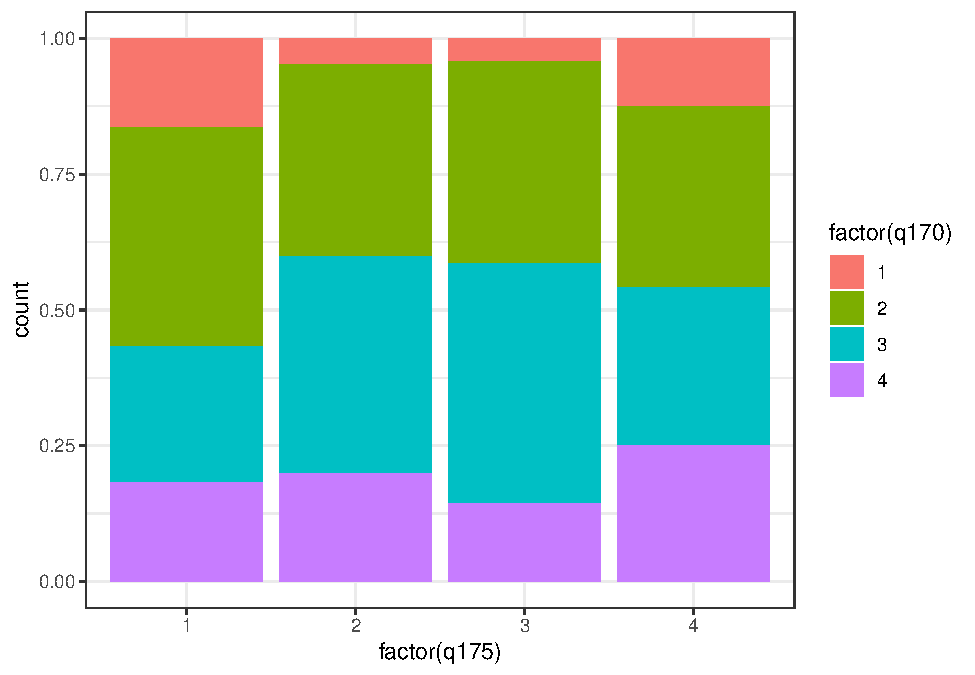
\includegraphics[keepaspectratio]{POL342-tutorial-notes_files/figure-latex/unnamed-chunk-274-1.pdf}}

\begin{Shaded}
\begin{Highlighting}[]
\NormalTok{df\_recode }\SpecialCharTok{|\textgreater{}}
  \FunctionTok{ggplot}\NormalTok{(}\FunctionTok{aes}\NormalTok{(}\AttributeTok{fill=}\FunctionTok{factor}\NormalTok{(q170),}\AttributeTok{x=}\FunctionTok{factor}\NormalTok{(q175))) }\SpecialCharTok{+}
  \FunctionTok{geom\_bar}\NormalTok{(}\AttributeTok{position=}\StringTok{"fill"}\NormalTok{) }\SpecialCharTok{+}
  \FunctionTok{theme\_bw}\NormalTok{() }\SpecialCharTok{+}
  \FunctionTok{scale\_fill\_manual}\NormalTok{(}\AttributeTok{name=}\StringTok{"Q170. Democratic}\SpecialCharTok{\textbackslash{}n}\StringTok{systems are not}\SpecialCharTok{\textbackslash{}n}\StringTok{effective"}\NormalTok{, }\CommentTok{\#legend label; \textasciigrave{}\textbackslash{}n\textasciigrave{} breaks line}
                    \AttributeTok{values =} \FunctionTok{c}\NormalTok{(}\StringTok{"navyblue"}\NormalTok{,}\StringTok{"blue"}\NormalTok{,}\StringTok{"skyblue"}\NormalTok{,}\StringTok{"grey"}\NormalTok{), }\CommentTok{\#color specification}
                    \AttributeTok{labels =} \FunctionTok{c}\NormalTok{(}\StringTok{"Strongly Agree"}\NormalTok{,}\StringTok{"Somewhat Agree"}\NormalTok{, }\StringTok{"Somewhat Disagree"}\NormalTok{, }\StringTok{"Strongly Disagree"}\NormalTok{)) }\CommentTok{\#legend specification}
\end{Highlighting}
\end{Shaded}

\pandocbounded{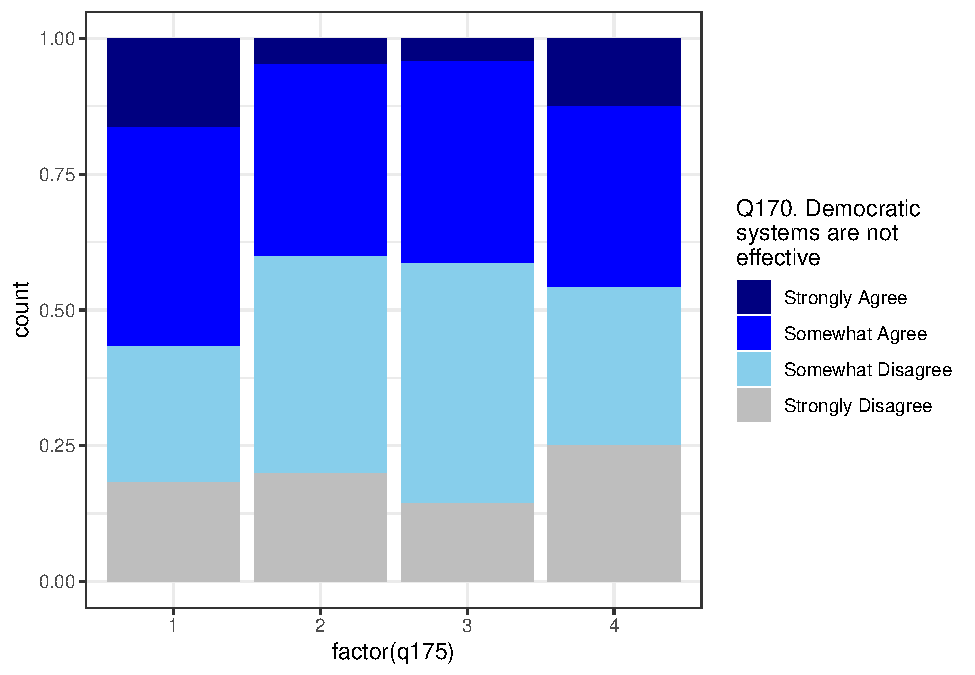
\includegraphics[keepaspectratio]{POL342-tutorial-notes_files/figure-latex/unnamed-chunk-275-1.pdf}}

\begin{Shaded}
\begin{Highlighting}[]
\NormalTok{df\_recode }\SpecialCharTok{|\textgreater{}}
  \FunctionTok{ggplot}\NormalTok{(}\FunctionTok{aes}\NormalTok{(}\AttributeTok{fill=}\FunctionTok{factor}\NormalTok{(q170),}\AttributeTok{x=}\FunctionTok{factor}\NormalTok{(q175))) }\SpecialCharTok{+}
  \FunctionTok{geom\_bar}\NormalTok{(}\AttributeTok{position=}\StringTok{"fill"}\NormalTok{) }\SpecialCharTok{+}
  \FunctionTok{theme\_bw}\NormalTok{() }\SpecialCharTok{+}
  \FunctionTok{scale\_fill\_manual}\NormalTok{(}\AttributeTok{name=}\StringTok{"Q170. Democratic}\SpecialCharTok{\textbackslash{}n}\StringTok{systems are not}\SpecialCharTok{\textbackslash{}n}\StringTok{effective"}\NormalTok{, }\CommentTok{\#legend label; \textasciigrave{}\textbackslash{}n\textasciigrave{} breaks line}
                    \AttributeTok{values =} \FunctionTok{c}\NormalTok{(}\StringTok{"navyblue"}\NormalTok{,}\StringTok{"blue"}\NormalTok{,}\StringTok{"skyblue"}\NormalTok{,}\StringTok{"grey"}\NormalTok{), }\CommentTok{\#color specification}
                    \AttributeTok{labels =} \FunctionTok{c}\NormalTok{(}\StringTok{"Strongly Agree"}\NormalTok{,}\StringTok{"Somewhat Agree"}\NormalTok{, }\StringTok{"Somewhat Disagree"}\NormalTok{, }\StringTok{"Strongly Disagree"}\NormalTok{)) }\SpecialCharTok{+} \CommentTok{\#legend specification}
  \FunctionTok{scale\_x\_discrete}\NormalTok{(}\AttributeTok{labels=}\FunctionTok{c}\NormalTok{(}\StringTok{"Much more good"}\NormalTok{, }\StringTok{"Somewhat more good"}\NormalTok{, }\StringTok{"Somewhat more harm"}\NormalTok{, }\StringTok{"Much more harm"}\NormalTok{),}
                   \AttributeTok{guide =} \FunctionTok{guide\_axis}\NormalTok{(}\AttributeTok{n.dodge=}\DecValTok{2}\NormalTok{)) }\SpecialCharTok{+}
  \FunctionTok{xlab}\NormalTok{(}\StringTok{"Q175. Does the United States do more good or harm to Asia?"}\NormalTok{) }\SpecialCharTok{+}
  \FunctionTok{ylab}\NormalTok{(}\StringTok{"Proportion"}\NormalTok{)}
\end{Highlighting}
\end{Shaded}

\pandocbounded{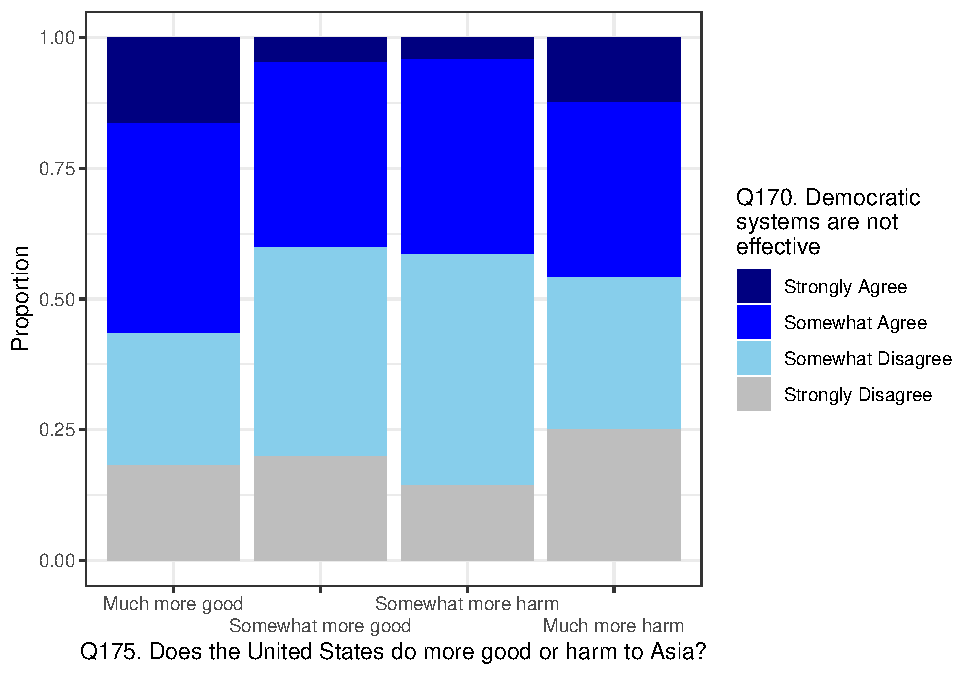
\includegraphics[keepaspectratio]{POL342-tutorial-notes_files/figure-latex/unnamed-chunk-276-1.pdf}}

\begin{Shaded}
\begin{Highlighting}[]
\NormalTok{df\_recode }\SpecialCharTok{|\textgreater{}}
  \FunctionTok{ggplot}\NormalTok{(}\FunctionTok{aes}\NormalTok{(}\AttributeTok{fill=}\FunctionTok{factor}\NormalTok{(q170),}\AttributeTok{x=}\FunctionTok{factor}\NormalTok{(q175))) }\SpecialCharTok{+}
  \FunctionTok{geom\_bar}\NormalTok{(}\AttributeTok{position=}\StringTok{"fill"}\NormalTok{) }\SpecialCharTok{+}
  \FunctionTok{theme\_bw}\NormalTok{() }\SpecialCharTok{+}
  \FunctionTok{scale\_fill\_manual}\NormalTok{(}\AttributeTok{name=}\StringTok{"Q170. Democratic}\SpecialCharTok{\textbackslash{}n}\StringTok{systems are not}\SpecialCharTok{\textbackslash{}n}\StringTok{effective"}\NormalTok{, }\CommentTok{\#legend label; \textasciigrave{}\textbackslash{}n\textasciigrave{} breaks line}
                    \AttributeTok{values =} \FunctionTok{c}\NormalTok{(}\StringTok{"navyblue"}\NormalTok{,}\StringTok{"blue"}\NormalTok{,}\StringTok{"skyblue"}\NormalTok{,}\StringTok{"grey"}\NormalTok{), }\CommentTok{\#color specification}
                    \AttributeTok{labels =} \FunctionTok{c}\NormalTok{(}\StringTok{"Strongly Agree"}\NormalTok{,}\StringTok{"Somewhat Agree"}\NormalTok{, }\StringTok{"Somewhat Disagree"}\NormalTok{, }\StringTok{"Strongly Disagree"}\NormalTok{)) }\SpecialCharTok{+} \CommentTok{\#legend specification}
  \FunctionTok{scale\_x\_discrete}\NormalTok{(}\AttributeTok{labels=}\FunctionTok{c}\NormalTok{(}\StringTok{"Much more good"}\NormalTok{, }\StringTok{"Somewhat more good"}\NormalTok{, }\StringTok{"Somewhat more harm"}\NormalTok{, }\StringTok{"Much more harm"}\NormalTok{),}
                   \AttributeTok{guide =} \FunctionTok{guide\_axis}\NormalTok{(}\AttributeTok{n.dodge=}\DecValTok{2}\NormalTok{)) }\SpecialCharTok{+}
  \FunctionTok{xlab}\NormalTok{(}\StringTok{"Q175. Does the United States do more good or harm to Asia?"}\NormalTok{) }\SpecialCharTok{+}
  \FunctionTok{ylab}\NormalTok{(}\StringTok{"Proportion"}\NormalTok{) }\SpecialCharTok{+}
  \FunctionTok{geom\_text}\NormalTok{(}\FunctionTok{aes}\NormalTok{(}\AttributeTok{x =} \FunctionTok{factor}\NormalTok{(q175), }\CommentTok{\# position along x axis follows q175}
                \AttributeTok{label =} \FunctionTok{round}\NormalTok{(}\FunctionTok{after\_stat}\NormalTok{(count }\SpecialCharTok{/} \FunctionTok{tapply}\NormalTok{(count, x, sum)[x]),}\DecValTok{3}\NormalTok{)), }\CommentTok{\# text}
            \AttributeTok{stat =} \StringTok{"count"}\NormalTok{,}
            \AttributeTok{position =} \FunctionTok{position\_fill}\NormalTok{(}\AttributeTok{vjust =}\NormalTok{ .}\DecValTok{5}\NormalTok{), }\CommentTok{\# position text at center of each fill block}
            \AttributeTok{color=}\StringTok{"white"}\NormalTok{)}
\end{Highlighting}
\end{Shaded}

\pandocbounded{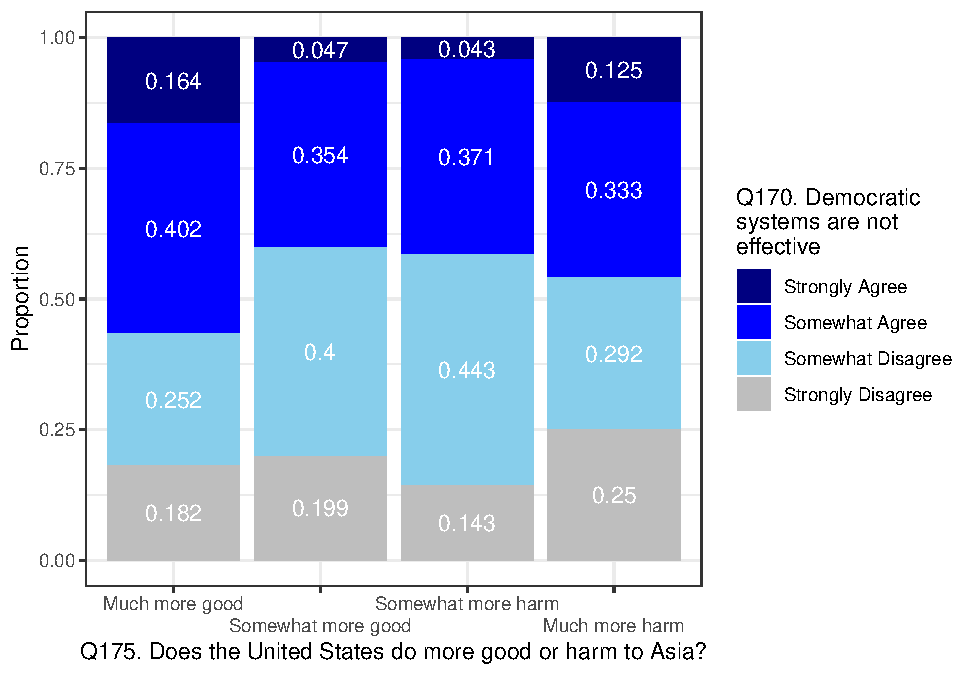
\includegraphics[keepaspectratio]{POL342-tutorial-notes_files/figure-latex/unnamed-chunk-277-1.pdf}}

\subsection*{Clear environment}\label{clear-environment-3}
\addcontentsline{toc}{subsection}{Clear environment}

\begin{Shaded}
\begin{Highlighting}[]
\FunctionTok{rm}\NormalTok{(}\AttributeTok{list=}\FunctionTok{ls}\NormalTok{())}
\end{Highlighting}
\end{Shaded}

\section{Box and whiskers plot}\label{box-and-whiskers-plot}

\subsection*{Prepare variables (CES)}\label{prepare-variables-ces}
\addcontentsline{toc}{subsection}{Prepare variables (CES)}

\begin{Shaded}
\begin{Highlighting}[]
\NormalTok{vars }\OtherTok{\textless{}{-}} \FunctionTok{c}\NormalTok{(}\StringTok{"pes21\_groups1\_4"}\NormalTok{,}\StringTok{"cps21\_news\_cons"}\NormalTok{,}\StringTok{"cps21\_govt\_confusing"}\NormalTok{) }\CommentTok{\#news consumption and internal political efficacy}

\NormalTok{ces\_select }\OtherTok{\textless{}{-}} \FunctionTok{read\_dta}\NormalTok{(}\StringTok{"Project/CES2021/2021 Canadian Election Study v2.0.dta"}\NormalTok{) }\SpecialCharTok{|\textgreater{}}
\NormalTok{  dplyr}\SpecialCharTok{::}\FunctionTok{select}\NormalTok{(}\FunctionTok{all\_of}\NormalTok{(vars))}

\NormalTok{ces\_dropna }\OtherTok{\textless{}{-}}\NormalTok{ ces\_select }\SpecialCharTok{|\textgreater{}}
  \FunctionTok{mutate}\NormalTok{(}\AttributeTok{cps21\_govt\_confusing=}\FunctionTok{ifelse}\NormalTok{(cps21\_govt\_confusing}\SpecialCharTok{==}\DecValTok{5}\NormalTok{, }\CommentTok{\#conditional statement}
                                     \ConstantTok{NA}\NormalTok{, }\CommentTok{\#if yes}
\NormalTok{                                     cps21\_govt\_confusing), }\CommentTok{\#if no}
         \AttributeTok{cps21\_news\_cons=}\FunctionTok{ifelse}\NormalTok{(cps21\_news\_cons}\SpecialCharTok{==}\DecValTok{7}\NormalTok{, }\CommentTok{\#conditional statement}
                                \ConstantTok{NA}\NormalTok{, }\CommentTok{\#if yes}
\NormalTok{                                cps21\_news\_cons), }\CommentTok{\#if no}
         \AttributeTok{pes21\_groups1\_4=}\FunctionTok{ifelse}\NormalTok{(pes21\_groups1\_4}\SpecialCharTok{\textless{}}\DecValTok{0}\NormalTok{,}
                                \ConstantTok{NA}\NormalTok{,}
\NormalTok{                                pes21\_groups1\_4)) }\SpecialCharTok{|\textgreater{}} 
  \FunctionTok{na.omit}\NormalTok{() }\CommentTok{\#remove NAs}
\end{Highlighting}
\end{Shaded}

\begin{Shaded}
\begin{Highlighting}[]
\FunctionTok{ggplot}\NormalTok{(ces\_dropna, }\FunctionTok{aes}\NormalTok{(}\AttributeTok{x=}\FunctionTok{factor}\NormalTok{(cps21\_govt\_confusing), }\AttributeTok{y=}\NormalTok{pes21\_groups1\_4)) }\SpecialCharTok{+}
  \FunctionTok{geom\_boxplot}\NormalTok{()}
\end{Highlighting}
\end{Shaded}

\pandocbounded{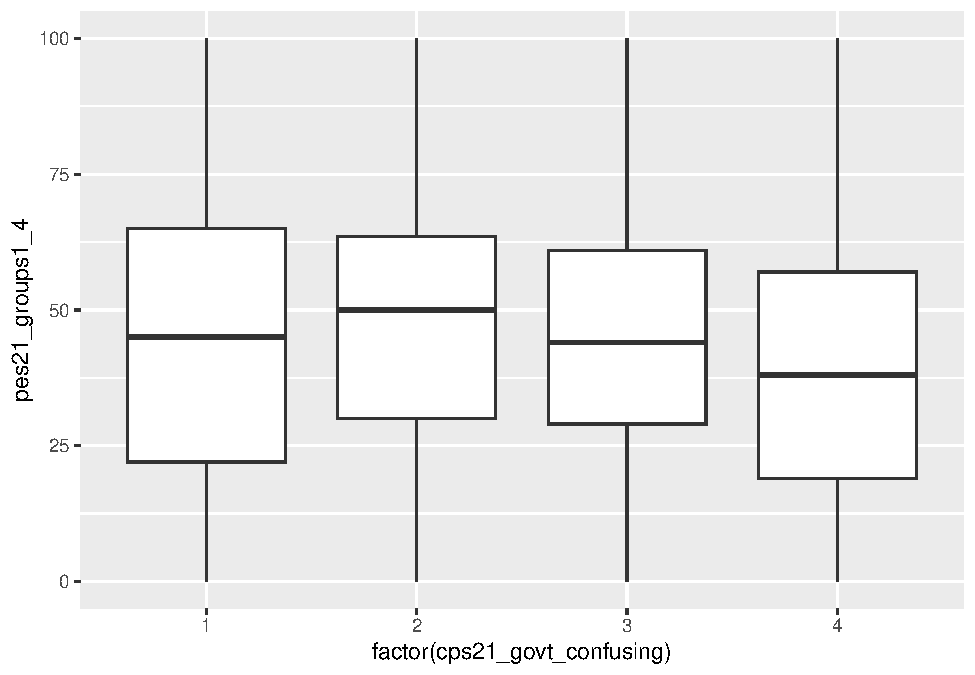
\includegraphics[keepaspectratio]{POL342-tutorial-notes_files/figure-latex/unnamed-chunk-280-1.pdf}}

\begin{itemize}
\tightlist
\item
  \texttt{width} in \texttt{geom\_boxplot} controls the width of the boxplot
\item
  \texttt{geom\_point(stat="summary,\ fun=mean)} adds a point plot of the conditional mean in addition to the quartiles noted in the box and whiskers
\item
  ggplot shapes for point or scatter
\end{itemize}

\begin{center}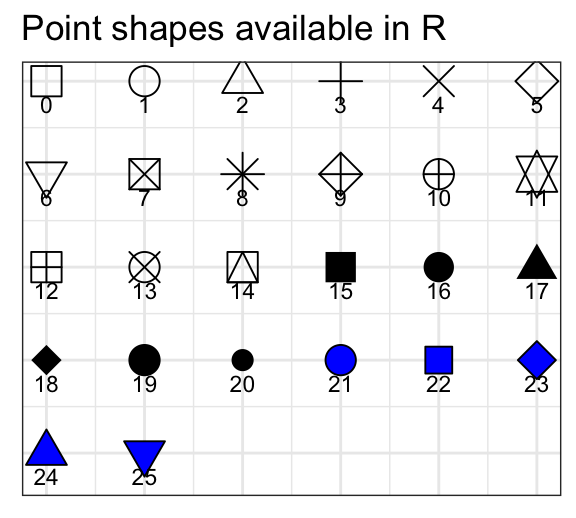
\includegraphics[width=0.6\linewidth]{images/w10_ggplot_shape} \end{center}

\begin{Shaded}
\begin{Highlighting}[]
\FunctionTok{ggplot}\NormalTok{(ces\_dropna, }\FunctionTok{aes}\NormalTok{(}\AttributeTok{x=}\FunctionTok{factor}\NormalTok{(cps21\_govt\_confusing), }\AttributeTok{y=}\NormalTok{pes21\_groups1\_4)) }\SpecialCharTok{+}
  \FunctionTok{geom\_boxplot}\NormalTok{(}\AttributeTok{width=}\FloatTok{0.3}\NormalTok{, }\AttributeTok{fill=}\StringTok{"darkseagreen"}\NormalTok{) }\SpecialCharTok{+}
  \FunctionTok{geom\_point}\NormalTok{(}\AttributeTok{stat=}\StringTok{"summary"}\NormalTok{, }\AttributeTok{fun=}\NormalTok{mean, }\AttributeTok{shape=}\DecValTok{23}\NormalTok{, }\AttributeTok{fill=}\StringTok{"black"}\NormalTok{,}\AttributeTok{size=}\FloatTok{2.5}\NormalTok{) }\SpecialCharTok{+}
  \FunctionTok{scale\_x\_discrete}\NormalTok{(}\AttributeTok{labels=}\FunctionTok{c}\NormalTok{(}\StringTok{"1}\SpecialCharTok{\textbackslash{}n}\StringTok{Strongly Disagree"}\NormalTok{,}\StringTok{"Somewhat Disagree"}\NormalTok{,}\StringTok{"Somewhat Agree"}\NormalTok{,}\StringTok{"4}\SpecialCharTok{\textbackslash{}n}\StringTok{Strongly Agree"}\NormalTok{)) }\SpecialCharTok{+}
  \FunctionTok{theme\_bw}\NormalTok{() }\SpecialCharTok{+}
  \FunctionTok{xlab}\NormalTok{(}\StringTok{"Sometimes, politics and government seem so complicated that a person}\SpecialCharTok{\textbackslash{}n}\StringTok{ like me can\textquotesingle{}t really understand what\textquotesingle{}s going on."}\NormalTok{) }\SpecialCharTok{+}
  \FunctionTok{ylab}\NormalTok{(}\StringTok{"How do you feel about the following groups in Canada}\SpecialCharTok{\textbackslash{}n}\StringTok{ [politicians in general]?"}\NormalTok{)}
\end{Highlighting}
\end{Shaded}

\pandocbounded{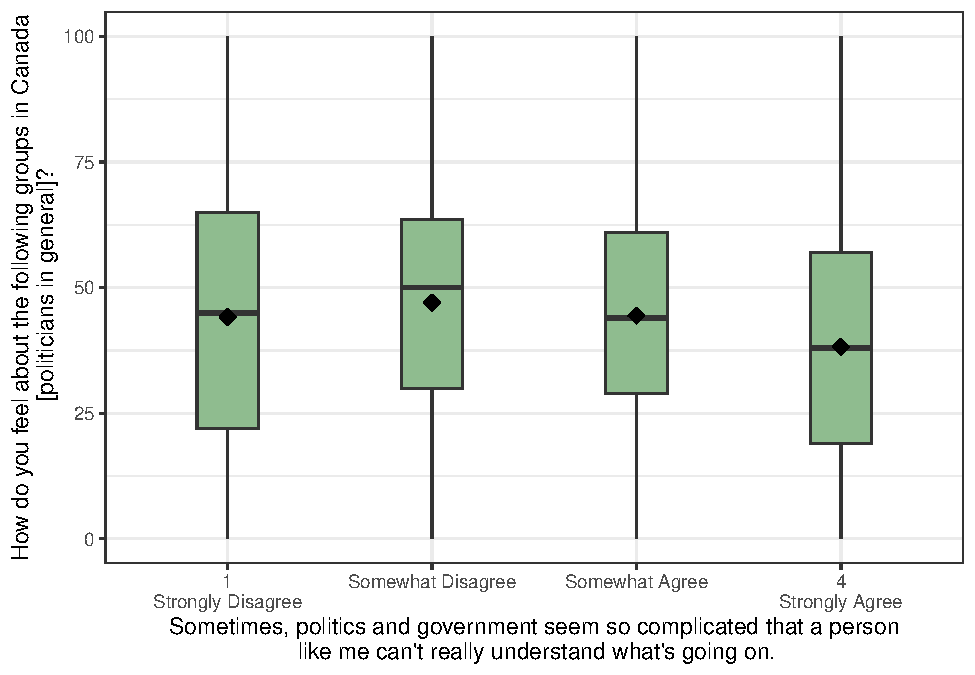
\includegraphics[keepaspectratio]{POL342-tutorial-notes_files/figure-latex/unnamed-chunk-282-1.pdf}}

\subsection*{Clear environment}\label{clear-environment-4}
\addcontentsline{toc}{subsection}{Clear environment}

\begin{Shaded}
\begin{Highlighting}[]
\FunctionTok{rm}\NormalTok{(}\AttributeTok{list=}\FunctionTok{ls}\NormalTok{())}
\end{Highlighting}
\end{Shaded}

\section{Scatter plot}\label{scatter-plot}

\subsection*{Prepare variables (VDem)}\label{prepare-variables-vdem}
\addcontentsline{toc}{subsection}{Prepare variables (VDem)}

\begin{Shaded}
\begin{Highlighting}[]
\NormalTok{vars }\OtherTok{\textless{}{-}} \FunctionTok{c}\NormalTok{(}\StringTok{"country\_name"}\NormalTok{, }\StringTok{"country\_id"}\NormalTok{, }\StringTok{"year"}\NormalTok{, }
          \StringTok{"e\_cow\_exports"}\NormalTok{,}\StringTok{"e\_gdppc"}\NormalTok{,}\StringTok{"e\_gdp"}\NormalTok{,}\StringTok{"e\_cow\_imports"}\NormalTok{,}\StringTok{"v2x\_pubcorr"}\NormalTok{)}

\NormalTok{vdem\_selected }\OtherTok{\textless{}{-}} \FunctionTok{read.csv}\NormalTok{(}\StringTok{"Project/VDem/VDem\_post2000.csv"}\NormalTok{) }\SpecialCharTok{|\textgreater{}}
  \FunctionTok{select}\NormalTok{(}\FunctionTok{all\_of}\NormalTok{(vars)) }\SpecialCharTok{|\textgreater{}}
  \FunctionTok{filter}\NormalTok{(year}\SpecialCharTok{==}\DecValTok{2014}\NormalTok{)}

\NormalTok{df }\OtherTok{\textless{}{-}}\NormalTok{ vdem\_selected }\SpecialCharTok{|\textgreater{}}
  \FunctionTok{mutate}\NormalTok{(}\AttributeTok{trade =}\NormalTok{ (e\_cow\_exports}\SpecialCharTok{+}\NormalTok{e\_cow\_imports)}\SpecialCharTok{/}\NormalTok{(e\_gdp)) }\CommentTok{\# trade volume as proportion of gdp}

\FunctionTok{ggplot}\NormalTok{(}\AttributeTok{data=}\NormalTok{df,}\FunctionTok{aes}\NormalTok{(}\AttributeTok{x=}\NormalTok{trade,}\AttributeTok{y=}\NormalTok{v2x\_pubcorr)) }\SpecialCharTok{+}
  \FunctionTok{geom\_point}\NormalTok{()}
\end{Highlighting}
\end{Shaded}

\pandocbounded{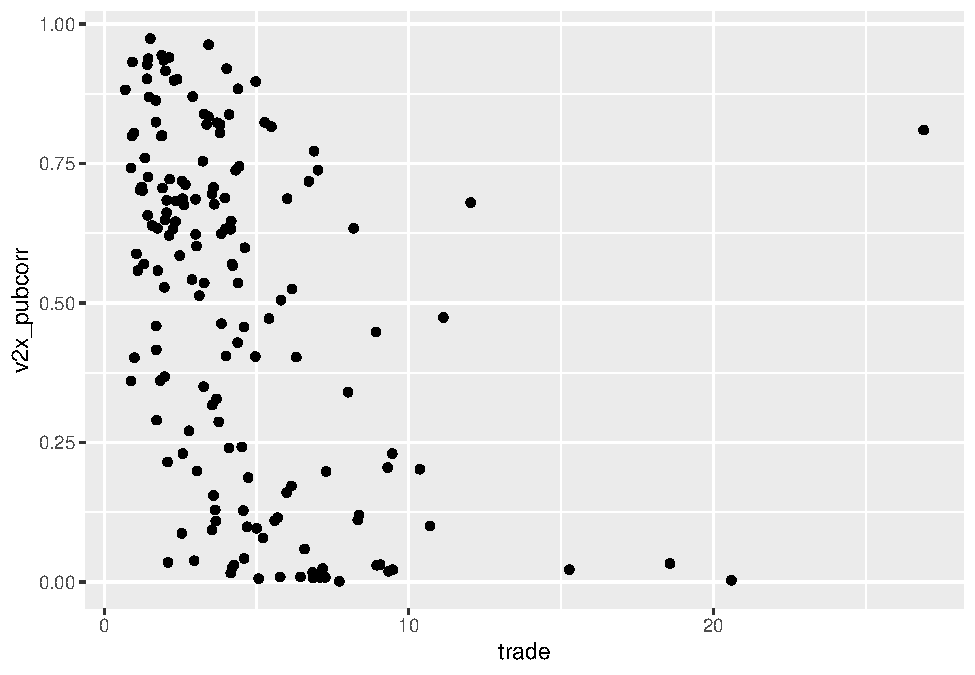
\includegraphics[keepaspectratio]{POL342-tutorial-notes_files/figure-latex/unnamed-chunk-284-1.pdf}}

\begin{Shaded}
\begin{Highlighting}[]
\FunctionTok{ggplot}\NormalTok{(}\AttributeTok{data=}\NormalTok{df,}\FunctionTok{aes}\NormalTok{(}\AttributeTok{x=}\FunctionTok{log}\NormalTok{(trade),}\AttributeTok{y=}\NormalTok{v2x\_pubcorr)) }\SpecialCharTok{+}
  \FunctionTok{geom\_point}\NormalTok{()}
\end{Highlighting}
\end{Shaded}

\pandocbounded{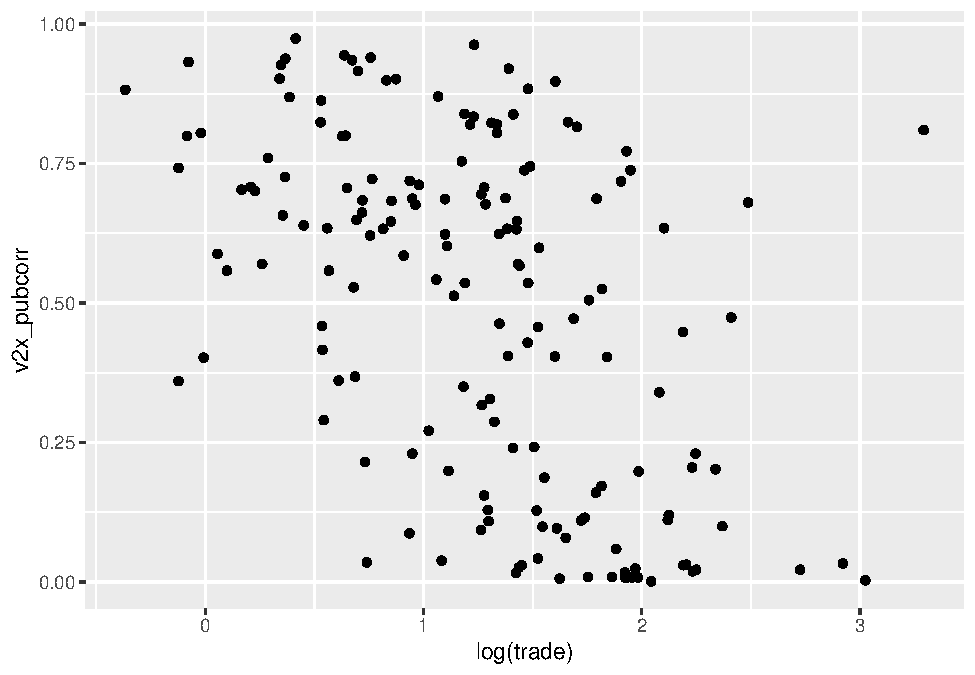
\includegraphics[keepaspectratio]{POL342-tutorial-notes_files/figure-latex/unnamed-chunk-284-2.pdf}}

\subsubsection*{Consider including your main control variable in the bivariate plot}\label{consider-including-your-main-control-variable-in-the-bivariate-plot}
\addcontentsline{toc}{subsubsection}{Consider including your main control variable in the bivariate plot}

For example, the bivariate scatter seems to support a theory that reliance of economy on trade is associated with lower levels of public sector corruption. However, when GDP per capita is included, the plot shows that countries that rely on trade also tend to be richer. In other words, we may not have sufficient variation to disentangle the effects of trade reliance from developed economies.

\begin{Shaded}
\begin{Highlighting}[]
\FunctionTok{ggplot}\NormalTok{(}\AttributeTok{data=}\NormalTok{df,}\FunctionTok{aes}\NormalTok{(}\AttributeTok{x=}\FunctionTok{log}\NormalTok{(trade),}\AttributeTok{y=}\NormalTok{v2x\_pubcorr)) }\SpecialCharTok{+}
  \FunctionTok{geom\_point}\NormalTok{(}\FunctionTok{aes}\NormalTok{(}\AttributeTok{color=}\FunctionTok{log}\NormalTok{(e\_gdppc)),}\AttributeTok{alpha=}\FloatTok{0.8}\NormalTok{,}\AttributeTok{size=}\DecValTok{2}\NormalTok{) }\SpecialCharTok{+}
  \FunctionTok{theme\_classic}\NormalTok{() }\SpecialCharTok{+}
  \FunctionTok{xlab}\NormalTok{(}\StringTok{"Trade volume as proportion of GDP"}\NormalTok{) }\SpecialCharTok{+}
  \FunctionTok{ylab}\NormalTok{(}\StringTok{"Public sector corruption"}\NormalTok{) }\SpecialCharTok{+}
  \FunctionTok{scale\_color\_gradient}\NormalTok{(}\AttributeTok{name=}\StringTok{"GDP per capita (logged)"}\NormalTok{,}
                       \AttributeTok{low=}\StringTok{"black"}\NormalTok{,}\AttributeTok{high=}\StringTok{"red"}\NormalTok{)}
\end{Highlighting}
\end{Shaded}

\pandocbounded{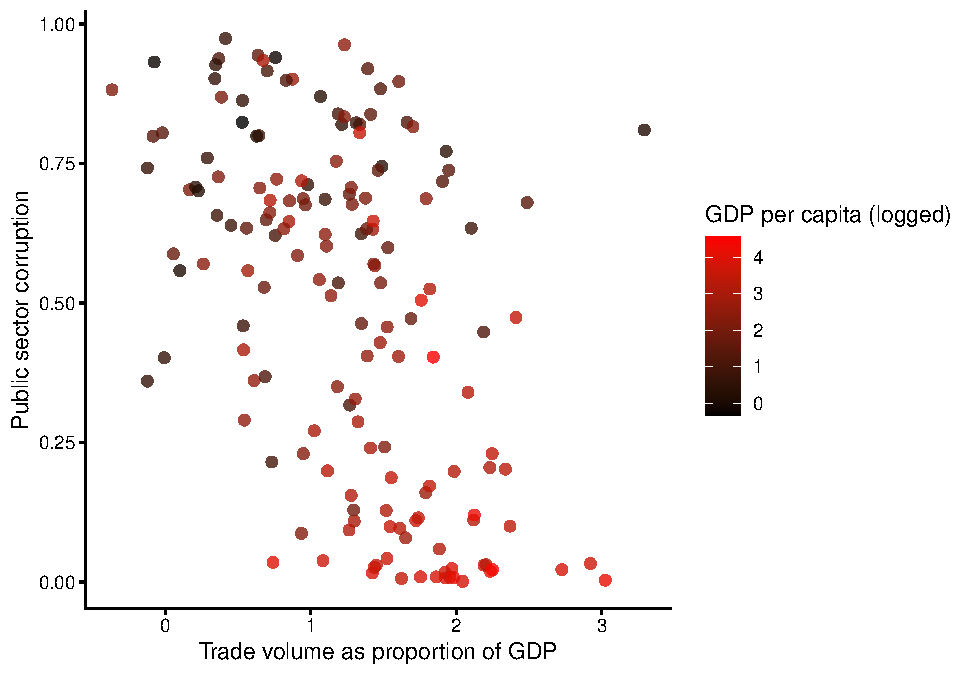
\includegraphics[keepaspectratio]{POL342-tutorial-notes_files/figure-latex/unnamed-chunk-285-1.pdf}}

\subsection*{\texorpdfstring{Saving plots using \texttt{ggsave()}}{Saving plots using ggsave()}}\label{saving-plots-using-ggsave}
\addcontentsline{toc}{subsection}{Saving plots using \texttt{ggsave()}}

\begin{Shaded}
\begin{Highlighting}[]
\CommentTok{\# save as object}
\NormalTok{plt }\OtherTok{\textless{}{-}} \FunctionTok{ggplot}\NormalTok{(}\AttributeTok{data=}\NormalTok{df,}\FunctionTok{aes}\NormalTok{(}\AttributeTok{x=}\FunctionTok{log}\NormalTok{(trade),}\AttributeTok{y=}\NormalTok{v2x\_pubcorr)) }\SpecialCharTok{+}
  \FunctionTok{geom\_point}\NormalTok{(}\FunctionTok{aes}\NormalTok{(}\AttributeTok{color=}\FunctionTok{log}\NormalTok{(e\_gdppc)),}\AttributeTok{alpha=}\FloatTok{0.8}\NormalTok{,}\AttributeTok{size=}\DecValTok{2}\NormalTok{) }\SpecialCharTok{+}
  \FunctionTok{theme\_classic}\NormalTok{() }\SpecialCharTok{+}
  \FunctionTok{xlab}\NormalTok{(}\StringTok{"Total trade per capita (logged)"}\NormalTok{) }\SpecialCharTok{+}
  \FunctionTok{ylab}\NormalTok{(}\StringTok{"Public sector corruption"}\NormalTok{) }\SpecialCharTok{+}
  \FunctionTok{scale\_color\_gradient}\NormalTok{(}\AttributeTok{name=}\StringTok{"GDP per capita (logged)"}\NormalTok{,}
                       \AttributeTok{low=}\StringTok{"black"}\NormalTok{,}\AttributeTok{high=}\StringTok{"red"}\NormalTok{)}

\CommentTok{\# use ggsave()}
\FunctionTok{ggsave}\NormalTok{(}\AttributeTok{filename=}\StringTok{"plt.png"}\NormalTok{,}\AttributeTok{plot=}\NormalTok{plt)}
\end{Highlighting}
\end{Shaded}

\subsection*{Using measures from other datasets}\label{using-measures-from-other-datasets}
\addcontentsline{toc}{subsection}{Using measures from other datasets}

If you want to include data from other data sets, you must receive approval from the TAs or Prof.~Besco prior to submission.

\begin{Shaded}
\begin{Highlighting}[]
\NormalTok{cowSL }\OtherTok{\textless{}{-}} \FunctionTok{read.csv}\NormalTok{(}\StringTok{"data/statelist2024.csv"}\NormalTok{)}
\FunctionTok{library}\NormalTok{(countrycode)}

\NormalTok{cowSL}\SpecialCharTok{$}\NormalTok{ccode\_vdem }\OtherTok{\textless{}{-}} \FunctionTok{countrycode}\NormalTok{(cowSL}\SpecialCharTok{$}\NormalTok{ccode,}
                                \AttributeTok{origin=}\StringTok{"cown"}\NormalTok{,}
                                \AttributeTok{destination=}\StringTok{"vdem"}\NormalTok{)}

\NormalTok{cowSL2 }\OtherTok{\textless{}{-}}\NormalTok{ cowSL }\SpecialCharTok{|\textgreater{}}
  \FunctionTok{filter}\NormalTok{(ccode\_vdem }\SpecialCharTok{\%in\%}\NormalTok{ vdem\_selected}\SpecialCharTok{$}\NormalTok{country\_id) }\SpecialCharTok{|\textgreater{}}
  \FunctionTok{group\_by}\NormalTok{(ccode) }\SpecialCharTok{|\textgreater{}}
  \FunctionTok{slice\_min}\NormalTok{(styear) }\CommentTok{\# using the earliest year for states that re{-}enter the system}

\NormalTok{df2 }\OtherTok{\textless{}{-}} \FunctionTok{left\_join}\NormalTok{(df, }
\NormalTok{          cowSL2[,}\FunctionTok{c}\NormalTok{(}\StringTok{"ccode\_vdem"}\NormalTok{,}\StringTok{"styear"}\NormalTok{)],}
          \AttributeTok{by=}\FunctionTok{c}\NormalTok{(}\StringTok{"country\_id"} \OtherTok{=} \StringTok{"ccode\_vdem"}\NormalTok{))}

\FunctionTok{ggplot}\NormalTok{(}\AttributeTok{data=}\NormalTok{df2,}\FunctionTok{aes}\NormalTok{(}\AttributeTok{x=}\FunctionTok{log}\NormalTok{(trade),}\AttributeTok{y=}\NormalTok{v2x\_pubcorr)) }\SpecialCharTok{+}
  \FunctionTok{geom\_point}\NormalTok{(}\FunctionTok{aes}\NormalTok{(}\AttributeTok{color=}\NormalTok{styear),}\AttributeTok{alpha=}\FloatTok{0.8}\NormalTok{,}\AttributeTok{size=}\DecValTok{2}\NormalTok{) }\SpecialCharTok{+}
  \FunctionTok{theme\_classic}\NormalTok{() }\SpecialCharTok{+}
  \FunctionTok{xlab}\NormalTok{(}\StringTok{"Trade volume as proportion of GDP"}\NormalTok{) }\SpecialCharTok{+}
  \FunctionTok{ylab}\NormalTok{(}\StringTok{"Public sector corruption"}\NormalTok{) }\SpecialCharTok{+}
  \FunctionTok{scale\_color\_gradient}\NormalTok{(}\AttributeTok{name=}\StringTok{"First year in state system"}\NormalTok{,}
                       \AttributeTok{low=}\StringTok{"black"}\NormalTok{,}\AttributeTok{high=}\StringTok{"red"}\NormalTok{)}
\end{Highlighting}
\end{Shaded}

\pandocbounded{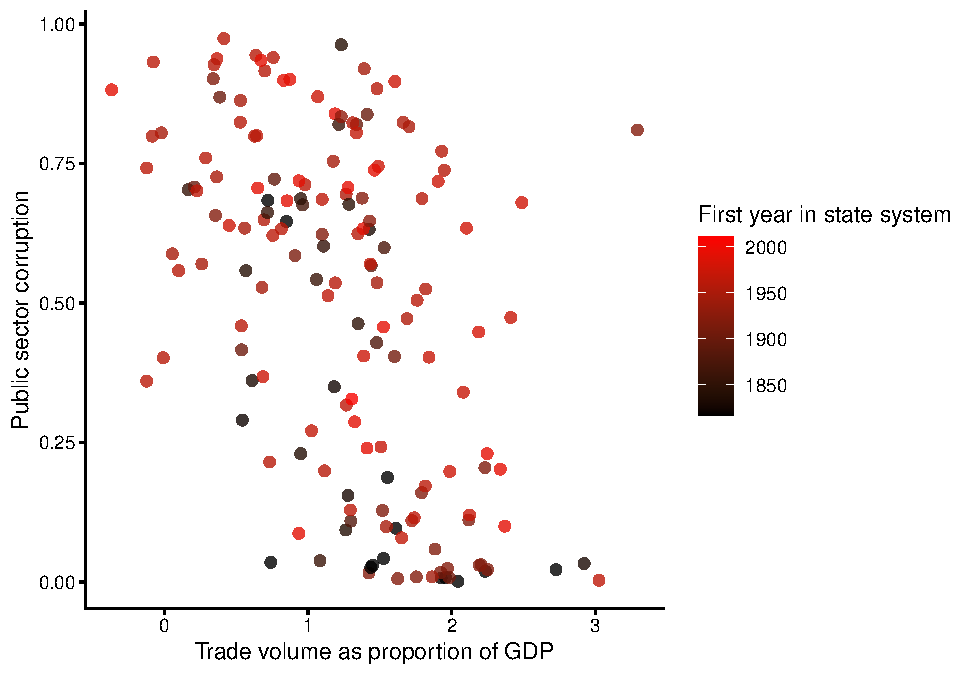
\includegraphics[keepaspectratio]{POL342-tutorial-notes_files/figure-latex/unnamed-chunk-287-1.pdf}}

\subsection*{Clear environment}\label{clear-environment-5}
\addcontentsline{toc}{subsection}{Clear environment}

\begin{Shaded}
\begin{Highlighting}[]
\FunctionTok{rm}\NormalTok{(}\AttributeTok{list=}\FunctionTok{ls}\NormalTok{())}
\end{Highlighting}
\end{Shaded}


\bibliography{book.bib,packages.bib}

\end{document}
